\documentclass[twoside]{book}

% Packages required by doxygen
\usepackage{fixltx2e}
\usepackage{calc}
\usepackage{doxygen}
\usepackage[export]{adjustbox} % also loads graphicx
\usepackage{graphicx}
\usepackage[utf8]{inputenc}
\usepackage{makeidx}
\usepackage{multicol}
\usepackage{multirow}
\PassOptionsToPackage{warn}{textcomp}
\usepackage{textcomp}
\usepackage[nointegrals]{wasysym}
\usepackage[table]{xcolor}

% Font selection
\usepackage[T1]{fontenc}
\usepackage[scaled=.90]{helvet}
\usepackage{courier}
\usepackage{amssymb}
\usepackage{sectsty}
\renewcommand{\familydefault}{\sfdefault}
\allsectionsfont{%
  \fontseries{bc}\selectfont%
  \color{darkgray}%
}
\renewcommand{\DoxyLabelFont}{%
  \fontseries{bc}\selectfont%
  \color{darkgray}%
}
\newcommand{\+}{\discretionary{\mbox{\scriptsize$\hookleftarrow$}}{}{}}

% Page & text layout
\usepackage{geometry}
\geometry{%
  a4paper,%
  top=2.5cm,%
  bottom=2.5cm,%
  left=2.5cm,%
  right=2.5cm%
}
\tolerance=750
\hfuzz=15pt
\hbadness=750
\setlength{\emergencystretch}{15pt}
\setlength{\parindent}{0cm}
\setlength{\parskip}{3ex plus 2ex minus 2ex}
\makeatletter
\renewcommand{\paragraph}{%
  \@startsection{paragraph}{4}{0ex}{-1.0ex}{1.0ex}{%
    \normalfont\normalsize\bfseries\SS@parafont%
  }%
}
\renewcommand{\subparagraph}{%
  \@startsection{subparagraph}{5}{0ex}{-1.0ex}{1.0ex}{%
    \normalfont\normalsize\bfseries\SS@subparafont%
  }%
}
\makeatother

% Headers & footers
\usepackage{fancyhdr}
\pagestyle{fancyplain}
\fancyhead[LE]{\fancyplain{}{\bfseries\thepage}}
\fancyhead[CE]{\fancyplain{}{}}
\fancyhead[RE]{\fancyplain{}{\bfseries\leftmark}}
\fancyhead[LO]{\fancyplain{}{\bfseries\rightmark}}
\fancyhead[CO]{\fancyplain{}{}}
\fancyhead[RO]{\fancyplain{}{\bfseries\thepage}}
\fancyfoot[LE]{\fancyplain{}{}}
\fancyfoot[CE]{\fancyplain{}{}}
\fancyfoot[RE]{\fancyplain{}{\bfseries\scriptsize Generated by Doxygen }}
\fancyfoot[LO]{\fancyplain{}{\bfseries\scriptsize Generated by Doxygen }}
\fancyfoot[CO]{\fancyplain{}{}}
\fancyfoot[RO]{\fancyplain{}{}}
\renewcommand{\footrulewidth}{0.4pt}
\renewcommand{\chaptermark}[1]{%
  \markboth{#1}{}%
}
\renewcommand{\sectionmark}[1]{%
  \markright{\thesection\ #1}%
}

% Indices & bibliography
\usepackage{natbib}
\usepackage[titles]{tocloft}
\setcounter{tocdepth}{3}
\setcounter{secnumdepth}{5}
\makeindex

% Hyperlinks (required, but should be loaded last)
\usepackage{ifpdf}
\ifpdf
  \usepackage[pdftex,pagebackref=true]{hyperref}
\else
  \usepackage[ps2pdf,pagebackref=true]{hyperref}
\fi
\hypersetup{%
  colorlinks=true,%
  linkcolor=blue,%
  citecolor=blue,%
  unicode%
}

% Custom commands
\newcommand{\clearemptydoublepage}{%
  \newpage{\pagestyle{empty}\cleardoublepage}%
}

\usepackage{caption}
\captionsetup{labelsep=space,justification=centering,font={bf},singlelinecheck=off,skip=4pt,position=top}

%===== C O N T E N T S =====

\begin{document}

% Titlepage & ToC
\hypersetup{pageanchor=false,
             bookmarksnumbered=true,
             pdfencoding=unicode
            }
\pagenumbering{roman}
\begin{titlepage}
\vspace*{7cm}
\begin{center}%
{\Large Robosample }\\
\vspace*{1cm}
{\large Generated by Doxygen 1.8.11}\\
\end{center}
\end{titlepage}
\clearemptydoublepage
\tableofcontents
\clearemptydoublepage
\pagenumbering{arabic}
\hypersetup{pageanchor=true}

%--- Begin generated contents ---
\chapter{Hierarchical Index}
\section{Class Hierarchy}
This inheritance list is sorted roughly, but not completely, alphabetically\+:\begin{DoxyCompactList}
\item \contentsline{section}{\+\_\+fcomplex}{\pageref{struct__fcomplex}}{}
\item \contentsline{section}{b\+Arg\+Parser}{\pageref{classbArgParser}}{}
\item \contentsline{section}{b\+Specific\+Atom}{\pageref{classbSpecificAtom}}{}
\item Compound\begin{DoxyCompactList}
\item \contentsline{section}{Topology}{\pageref{classTopology}}{}
\end{DoxyCompactList}
\item \contentsline{section}{Context}{\pageref{classContext}}{}
\item Decoration\+Generator\begin{DoxyCompactList}
\item \contentsline{section}{Para\+Molecular\+Decorator}{\pageref{classParaMolecularDecorator}}{}
\end{DoxyCompactList}
\item \contentsline{section}{G\+C\+H\+M\+C\+Integrator}{\pageref{classGCHMCIntegrator}}{}
\item Implementation\begin{DoxyCompactList}
\item \contentsline{section}{Fixman\+Torque}{\pageref{classFixmanTorque}}{}
\end{DoxyCompactList}
\item \contentsline{section}{intpair}{\pageref{classintpair}}{}
\begin{DoxyCompactList}
\item \contentsline{section}{b\+Bond}{\pageref{classbBond}}{}
\end{DoxyCompactList}
\item iostream\begin{DoxyCompactList}
\item \contentsline{section}{Robo\+I\+O\+Stream}{\pageref{classRoboIOStream}}{}
\end{DoxyCompactList}
\item \contentsline{section}{P\+D\+B\+Object}{\pageref{classPDBObject}}{}
\item \contentsline{section}{Point}{\pageref{structPoint}}{}
\item \contentsline{section}{read\+Amber\+Input}{\pageref{classreadAmberInput}}{}
\item \contentsline{section}{Sampler}{\pageref{classSampler}}{}
\begin{DoxyCompactList}
\item \contentsline{section}{Conformational\+Search}{\pageref{classConformationalSearch}}{}
\item \contentsline{section}{Monte\+Carlo\+Sampler}{\pageref{classMonteCarloSampler}}{}
\begin{DoxyCompactList}
\item \contentsline{section}{H\+M\+C\+Sampler}{\pageref{classHMCSampler}}{}
\begin{DoxyCompactList}
\item \contentsline{section}{Girolami\+Sampler}{\pageref{classGirolamiSampler}}{}
\item \contentsline{section}{L\+A\+H\+M\+C\+Sampler}{\pageref{classLAHMCSampler}}{}
\end{DoxyCompactList}
\item \contentsline{section}{Test\+H\+M\+C\+S\+OA}{\pageref{classTestHMCSOA}}{}
\end{DoxyCompactList}
\end{DoxyCompactList}
\item \contentsline{section}{Setup\+Reader}{\pageref{classSetupReader}}{}
\begin{DoxyCompactList}
\item \contentsline{section}{Derived\+Setup\+Reader}{\pageref{classDerivedSetupReader}}{}
\end{DoxyCompactList}
\item Single\+Atom\begin{DoxyCompactList}
\item \contentsline{section}{Trivalent\+Atom\+Tetra}{\pageref{classTrivalentAtomTetra}}{}
\end{DoxyCompactList}
\item State\begin{DoxyCompactList}
\item \contentsline{section}{I\+State}{\pageref{classIState}}{}
\begin{DoxyCompactList}
\item \contentsline{section}{My\+State}{\pageref{classMyState}}{}
\end{DoxyCompactList}
\end{DoxyCompactList}
\item Task\begin{DoxyCompactList}
\item \contentsline{section}{Nonbonded\+Force\+Task}{\pageref{classNonbondedForceTask}}{}
\end{DoxyCompactList}
\item \contentsline{section}{Trajectory\+Object}{\pageref{classTrajectoryObject}}{}
\item \contentsline{section}{World}{\pageref{classWorld}}{}
\end{DoxyCompactList}

\chapter{Class Index}
\section{Class List}
Here are the classes, structs, unions and interfaces with brief descriptions\+:\begin{DoxyCompactList}
\item\contentsline{section}{\hyperlink{struct__fcomplex}{\+\_\+fcomplex} }{\pageref{struct__fcomplex}}{}
\item\contentsline{section}{\hyperlink{classbArgParser}{b\+Arg\+Parser} }{\pageref{classbArgParser}}{}
\item\contentsline{section}{\hyperlink{classbBond}{b\+Bond} }{\pageref{classbBond}}{}
\item\contentsline{section}{\hyperlink{classbSpecificAtom}{b\+Specific\+Atom} }{\pageref{classbSpecificAtom}}{}
\item\contentsline{section}{\hyperlink{classConformationalSearch}{Conformational\+Search} }{\pageref{classConformationalSearch}}{}
\item\contentsline{section}{\hyperlink{classContext}{Context} }{\pageref{classContext}}{}
\item\contentsline{section}{\hyperlink{classDerivedSetupReader}{Derived\+Setup\+Reader} }{\pageref{classDerivedSetupReader}}{}
\item\contentsline{section}{\hyperlink{classFixmanTorque}{Fixman\+Torque} }{\pageref{classFixmanTorque}}{}
\item\contentsline{section}{\hyperlink{classGCHMCIntegrator}{G\+C\+H\+M\+C\+Integrator} }{\pageref{classGCHMCIntegrator}}{}
\item\contentsline{section}{\hyperlink{classGirolamiSampler}{Girolami\+Sampler} }{\pageref{classGirolamiSampler}}{}
\item\contentsline{section}{\hyperlink{classHMCSampler}{H\+M\+C\+Sampler} }{\pageref{classHMCSampler}}{}
\item\contentsline{section}{\hyperlink{classintpair}{intpair} }{\pageref{classintpair}}{}
\item\contentsline{section}{\hyperlink{classIState}{I\+State} }{\pageref{classIState}}{}
\item\contentsline{section}{\hyperlink{classLAHMCSampler}{L\+A\+H\+M\+C\+Sampler} }{\pageref{classLAHMCSampler}}{}
\item\contentsline{section}{\hyperlink{classMonteCarloSampler}{Monte\+Carlo\+Sampler} }{\pageref{classMonteCarloSampler}}{}
\item\contentsline{section}{\hyperlink{classMyState}{My\+State} }{\pageref{classMyState}}{}
\item\contentsline{section}{\hyperlink{classNonbondedForceTask}{Nonbonded\+Force\+Task} }{\pageref{classNonbondedForceTask}}{}
\item\contentsline{section}{\hyperlink{classParaMolecularDecorator}{Para\+Molecular\+Decorator} }{\pageref{classParaMolecularDecorator}}{}
\item\contentsline{section}{\hyperlink{classPDBObject}{P\+D\+B\+Object} }{\pageref{classPDBObject}}{}
\item\contentsline{section}{\hyperlink{structPoint}{Point} }{\pageref{structPoint}}{}
\item\contentsline{section}{\hyperlink{classreadAmberInput}{read\+Amber\+Input} }{\pageref{classreadAmberInput}}{}
\item\contentsline{section}{\hyperlink{classRoboIOStream}{Robo\+I\+O\+Stream} }{\pageref{classRoboIOStream}}{}
\item\contentsline{section}{\hyperlink{classSampler}{Sampler} }{\pageref{classSampler}}{}
\item\contentsline{section}{\hyperlink{classSetupReader}{Setup\+Reader} }{\pageref{classSetupReader}}{}
\item\contentsline{section}{\hyperlink{classTestHMCSOA}{Test\+H\+M\+C\+S\+OA} }{\pageref{classTestHMCSOA}}{}
\item\contentsline{section}{\hyperlink{classTopology}{Topology} }{\pageref{classTopology}}{}
\item\contentsline{section}{\hyperlink{classTrajectoryObject}{Trajectory\+Object} }{\pageref{classTrajectoryObject}}{}
\item\contentsline{section}{\hyperlink{classTrivalentAtomTetra}{Trivalent\+Atom\+Tetra} }{\pageref{classTrivalentAtomTetra}}{}
\item\contentsline{section}{\hyperlink{classWorld}{World} }{\pageref{classWorld}}{}
\end{DoxyCompactList}

\chapter{File Index}
\section{File List}
Here is a list of all documented files with brief descriptions\+:\begin{DoxyCompactList}
\item\contentsline{section}{include/gmolmodel/{\bfseries b\+Arg\+Parser.\+hpp} }{\pageref{bArgParser_8hpp}}{}
\item\contentsline{section}{include/gmolmodel/\hyperlink{bBond_8hpp}{b\+Bond.\+hpp} }{\pageref{bBond_8hpp}}{}
\item\contentsline{section}{include/gmolmodel/{\bfseries bgeneral.\+hpp} }{\pageref{bgeneral_8hpp}}{}
\item\contentsline{section}{include/gmolmodel/\hyperlink{bSpecificAtom_8hpp}{b\+Specific\+Atom.\+hpp} }{\pageref{bSpecificAtom_8hpp}}{}
\item\contentsline{section}{include/gmolmodel/{\bfseries Conformational\+Search.\+hpp} }{\pageref{ConformationalSearch_8hpp}}{}
\item\contentsline{section}{include/gmolmodel/{\bfseries Context.\+hpp} }{\pageref{Context_8hpp}}{}
\item\contentsline{section}{include/gmolmodel/{\bfseries Fixman\+Torque.\+hpp} }{\pageref{FixmanTorque_8hpp}}{}
\item\contentsline{section}{include/gmolmodel/{\bfseries Girolami\+Sampler.\+hpp} }{\pageref{GirolamiSampler_8hpp}}{}
\item\contentsline{section}{include/gmolmodel/{\bfseries H\+M\+C\+Sampler.\+hpp} }{\pageref{HMCSampler_8hpp}}{}
\item\contentsline{section}{include/gmolmodel/{\bfseries H\+M\+C\+S\+O\+A.\+hpp} }{\pageref{HMCSOA_8hpp}}{}
\item\contentsline{section}{include/gmolmodel/{\bfseries I\+State.\+hpp} }{\pageref{IState_8hpp}}{}
\item\contentsline{section}{include/gmolmodel/{\bfseries L\+A\+H\+M\+C\+Sampler.\+hpp} }{\pageref{LAHMCSampler_8hpp}}{}
\item\contentsline{section}{include/gmolmodel/{\bfseries Monte\+Carlo\+Sampler.\+hpp} }{\pageref{MonteCarloSampler_8hpp}}{}
\item\contentsline{section}{include/gmolmodel/{\bfseries My\+State.\+hpp} }{\pageref{MyState_8hpp}}{}
\item\contentsline{section}{include/gmolmodel/{\bfseries Para\+Molecular\+Decorator.\+hpp} }{\pageref{ParaMolecularDecorator_8hpp}}{}
\item\contentsline{section}{include/gmolmodel/{\bfseries read\+Amber\+Input.\+hpp} }{\pageref{readAmberInput_8hpp}}{}
\item\contentsline{section}{include/gmolmodel/{\bfseries Robo.\+hpp} }{\pageref{Robo_8hpp}}{}
\item\contentsline{section}{include/gmolmodel/{\bfseries Robo\+I\+O\+Stream.\+hpp} }{\pageref{RoboIOStream_8hpp}}{}
\item\contentsline{section}{include/gmolmodel/{\bfseries Sampler.\+hpp} }{\pageref{Sampler_8hpp}}{}
\item\contentsline{section}{include/gmolmodel/{\bfseries server.\+hpp} }{\pageref{server_8hpp}}{}
\item\contentsline{section}{include/gmolmodel/{\bfseries Setup\+Reader.\+hpp} }{\pageref{SetupReader_8hpp}}{}
\item\contentsline{section}{include/gmolmodel/{\bfseries simmain.\+hpp} }{\pageref{simmain_8hpp}}{}
\item\contentsline{section}{include/gmolmodel/{\bfseries Topology.\+hpp} }{\pageref{Topology_8hpp}}{}
\item\contentsline{section}{include/gmolmodel/\hyperlink{TrivalentAtomTetra_8hpp}{Trivalent\+Atom\+Tetra.\+hpp} }{\pageref{TrivalentAtomTetra_8hpp}}{}
\item\contentsline{section}{include/gmolmodel/{\bfseries World.\+hpp} }{\pageref{World_8hpp}}{}
\item\contentsline{section}{include/gmolmodel/format/{\bfseries P\+D\+B\+Object.\+hpp} }{\pageref{PDBObject_8hpp}}{}
\item\contentsline{section}{include/gmolmodel/format/{\bfseries Trajectory\+Object.\+hpp} }{\pageref{TrajectoryObject_8hpp}}{}
\item\contentsline{section}{src/\hyperlink{bArgParser_8cpp}{b\+Arg\+Parser.\+cpp} }{\pageref{bArgParser_8cpp}}{}
\item\contentsline{section}{src/\hyperlink{ConformationalSearch_8cpp}{Conformational\+Search.\+cpp} }{\pageref{ConformationalSearch_8cpp}}{}
\item\contentsline{section}{src/\hyperlink{GirolamiSampler_8cpp}{Girolami\+Sampler.\+cpp} }{\pageref{GirolamiSampler_8cpp}}{}
\item\contentsline{section}{src/\hyperlink{HMCSampler_8cpp}{H\+M\+C\+Sampler.\+cpp} }{\pageref{HMCSampler_8cpp}}{}
\item\contentsline{section}{src/\hyperlink{LAHMCSampler_8cpp}{L\+A\+H\+M\+C\+Sampler.\+cpp} }{\pageref{LAHMCSampler_8cpp}}{}
\item\contentsline{section}{src/\hyperlink{MonteCarloSampler_8cpp}{Monte\+Carlo\+Sampler.\+cpp} }{\pageref{MonteCarloSampler_8cpp}}{}
\item\contentsline{section}{src/\hyperlink{ParaMolecularDecorator_8cpp}{Para\+Molecular\+Decorator.\+cpp} }{\pageref{ParaMolecularDecorator_8cpp}}{}
\item\contentsline{section}{src/\hyperlink{Sampler_8cpp}{Sampler.\+cpp} }{\pageref{Sampler_8cpp}}{}
\item\contentsline{section}{src/\hyperlink{Topology_8cpp}{Topology.\+cpp} }{\pageref{Topology_8cpp}}{}
\item\contentsline{section}{tests/\hyperlink{Robosample_8cpp}{Robosample.\+cpp} }{\pageref{Robosample_8cpp}}{}
\end{DoxyCompactList}

\chapter{Class Documentation}
\hypertarget{struct__fcomplex}{}\section{\+\_\+fcomplex Struct Reference}
\label{struct__fcomplex}\index{\+\_\+fcomplex@{\+\_\+fcomplex}}
\subsection*{Public Attributes}
\begin{DoxyCompactItemize}
\item 
float {\bfseries re}\hypertarget{struct__fcomplex_a2a0b3a27cdca39b44baa7d0f40738623}{}\label{struct__fcomplex_a2a0b3a27cdca39b44baa7d0f40738623}

\item 
float {\bfseries im}\hypertarget{struct__fcomplex_a703839cffd5c774188a01627a71b4a20}{}\label{struct__fcomplex_a703839cffd5c774188a01627a71b4a20}

\end{DoxyCompactItemize}


The documentation for this struct was generated from the following file\+:\begin{DoxyCompactItemize}
\item 
tests/Test\+Matrix.\+cpp\end{DoxyCompactItemize}

\hypertarget{classbArgParser}{}\section{b\+Arg\+Parser Class Reference}
\label{classbArgParser}\index{b\+Arg\+Parser@{b\+Arg\+Parser}}


{\ttfamily \#include $<$b\+Arg\+Parser.\+hpp$>$}

\subsection*{Public Types}
\begin{DoxyCompactItemize}
\item 
enum \{ {\bfseries A\+R\+\_\+\+L\+I\+G\+D\+IR}, 
{\bfseries A\+R\+\_\+\+G\+A\+FF}, 
{\bfseries A\+R\+\_\+\+I\+C\+TD}
 \}\hypertarget{classbArgParser_a056368260109e1fd1f62563fee5a908c}{}\label{classbArgParser_a056368260109e1fd1f62563fee5a908c}

\end{DoxyCompactItemize}
\subsection*{Public Member Functions}
\begin{DoxyCompactItemize}
\item 
{\bfseries b\+Arg\+Parser} (int argc, const char $\ast$$\ast$argv)\hypertarget{classbArgParser_a30d2a3f26dfb3632aa68b314955385c3}{}\label{classbArgParser_a30d2a3f26dfb3632aa68b314955385c3}

\item 
void {\bfseries Print} (void)\hypertarget{classbArgParser_ade060fb35d5828d57513674c27e7bfd8}{}\label{classbArgParser_ade060fb35d5828d57513674c27e7bfd8}

\end{DoxyCompactItemize}
\subsection*{Public Attributes}
\begin{DoxyCompactItemize}
\item 
int {\bfseries M\+A\+X\+\_\+\+N\+O\+\_\+\+O\+PT}\hypertarget{classbArgParser_a7cca8cd7c79c5e6d5a61bddec8ca6158}{}\label{classbArgParser_a7cca8cd7c79c5e6d5a61bddec8ca6158}

\item 
int $\ast$ {\bfseries option}\hypertarget{classbArgParser_a299ef19294e93f7f592916778b3d995f}{}\label{classbArgParser_a299ef19294e93f7f592916778b3d995f}

\item 
std\+::string {\bfseries mol2F}\hypertarget{classbArgParser_aebb226c57803a0345a10e38c2d477f2a}{}\label{classbArgParser_aebb226c57803a0345a10e38c2d477f2a}

\item 
std\+::string {\bfseries rbF}\hypertarget{classbArgParser_a9cf67edfd6b697ac460150bc1ccc88ac}{}\label{classbArgParser_a9cf67edfd6b697ac460150bc1ccc88ac}

\item 
std\+::string {\bfseries gaffF}\hypertarget{classbArgParser_a981bb3ee56f64fcedb2deee33d8dacbc}{}\label{classbArgParser_a981bb3ee56f64fcedb2deee33d8dacbc}

\item 
std\+::string {\bfseries frcmodF}\hypertarget{classbArgParser_a83d6b64d3e3e39796b2cdee9a41e8391}{}\label{classbArgParser_a83d6b64d3e3e39796b2cdee9a41e8391}

\item 
std\+::string {\bfseries ictdF}\hypertarget{classbArgParser_aa09c7af4426691f7c0bfaac27fd1ba80}{}\label{classbArgParser_aa09c7af4426691f7c0bfaac27fd1ba80}

\end{DoxyCompactItemize}


\subsection{Detailed Description}
Argument Parser Class. It is used by the \hyperlink{classGCHMCIntegrator}{G\+C\+H\+M\+C\+Integrator} class in simmain. It holds the pathnames of the files needed to construct the compound\+: a mol2 file, a rigid body specification file, the Amber gaff file and the type of dynamics that it supposed to be done. 

The documentation for this class was generated from the following files\+:\begin{DoxyCompactItemize}
\item 
include/gmolmodel/b\+Arg\+Parser.\+hpp\item 
src/\hyperlink{bArgParser_8cpp}{b\+Arg\+Parser.\+cpp}\end{DoxyCompactItemize}

\hypertarget{classbBond}{}\section{b\+Bond Class Reference}
\label{classbBond}\index{b\+Bond@{b\+Bond}}


{\ttfamily \#include $<$b\+Bond.\+hpp$>$}



Inheritance diagram for b\+Bond\+:\nopagebreak
\begin{figure}[H]
\begin{center}
\leavevmode
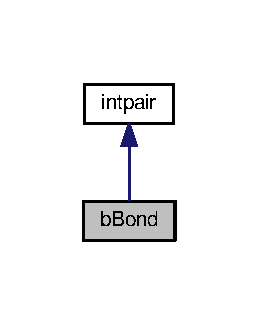
\includegraphics[width=124pt]{classbBond__inherit__graph}
\end{center}
\end{figure}


Collaboration diagram for b\+Bond\+:\nopagebreak
\begin{figure}[H]
\begin{center}
\leavevmode
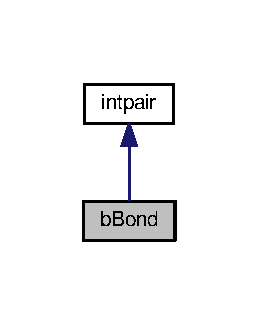
\includegraphics[width=124pt]{classbBond__coll__graph}
\end{center}
\end{figure}
\subsection*{Public Member Functions}
\begin{DoxyCompactItemize}
\item 
{\bfseries b\+Bond} (int a, int b)\hypertarget{classbBond_a1cda4467d17196755fb22093830f4d40}{}\label{classbBond_a1cda4467d17196755fb22093830f4d40}

\item 
bool {\bfseries is\+In\+Ring} (void)\hypertarget{classbBond_a7b050c59b5ca77c66bda45c344487236}{}\label{classbBond_a7b050c59b5ca77c66bda45c344487236}

\item 
bool {\bfseries is\+Ring\+Closing} (void)\hypertarget{classbBond_a45c45e0a9f77bb8d4ecf2f61a14e5d1d}{}\label{classbBond_a45c45e0a9f77bb8d4ecf2f61a14e5d1d}

\item 
const Sim\+T\+K\+::\+Bond\+Mobility\+::\+Mobility {\bfseries get\+Bond\+Mobility} () const \hypertarget{classbBond_a3e91f9e1c87dc954a29e35dee1212638}{}\label{classbBond_a3e91f9e1c87dc954a29e35dee1212638}

\item 
int {\bfseries ring\+No} (void)\hypertarget{classbBond_a1ee34276aab47e506f232d040fb0c32a}{}\label{classbBond_a1ee34276aab47e506f232d040fb0c32a}

\item 
void {\bfseries set\+In\+Ring} (void)\hypertarget{classbBond_a12acb32aad78703b8aab53626eac2680}{}\label{classbBond_a12acb32aad78703b8aab53626eac2680}

\item 
void {\bfseries set\+As\+Ring\+Closing} (void)\hypertarget{classbBond_abc744708c12f75f917f4d9d881829978}{}\label{classbBond_abc744708c12f75f917f4d9d881829978}

\item 
void {\bfseries set\+Bond\+Mobility} (Sim\+T\+K\+::\+Bond\+Mobility\+::\+Mobility some\+Mobility)\hypertarget{classbBond_a9bdeb22d5e5edd5e5aaf126c9ccbe7c8}{}\label{classbBond_a9bdeb22d5e5edd5e5aaf126c9ccbe7c8}

\item 
void {\bfseries set\+Ring\+No} (int rn)\hypertarget{classbBond_ad0489880ce030239bbef3768b23dfa6d}{}\label{classbBond_ad0489880ce030239bbef3768b23dfa6d}

\item 
Sim\+T\+K\+::\+Compound\+::\+Bond\+Index {\bfseries get\+Bond\+Index} (void)\hypertarget{classbBond_ad60a8e3207a98bcf593eb30441f1ce24}{}\label{classbBond_ad60a8e3207a98bcf593eb30441f1ce24}

\item 
void {\bfseries set\+Bond\+Index} (Sim\+T\+K\+::\+Compound\+::\+Bond\+Index other\+Ix)\hypertarget{classbBond_a81dd4c869c5d8fd841ce8edda2a42efa}{}\label{classbBond_a81dd4c869c5d8fd841ce8edda2a42efa}

\item 
void {\bfseries set\+Index} (int)\hypertarget{classbBond_a5b084292de272b7f6752183a275719c9}{}\label{classbBond_a5b084292de272b7f6752183a275719c9}

\item 
int {\bfseries get\+Index} (void)\hypertarget{classbBond_ac85ff74475b2b00206acd69a1a09481c}{}\label{classbBond_ac85ff74475b2b00206acd69a1a09481c}

\item 
void {\bfseries Print} (void)\hypertarget{classbBond_a23a5f3abe2f6a867e7343ef32f09d168}{}\label{classbBond_a23a5f3abe2f6a867e7343ef32f09d168}

\item 
bool {\bfseries is\+First} (void)\hypertarget{classbBond_a056c61e9e3238ff555dc041ec595ee80}{}\label{classbBond_a056c61e9e3238ff555dc041ec595ee80}

\item 
void {\bfseries set\+As\+First} (void)\hypertarget{classbBond_ab84068eecf02ee75a018181034f4c57b}{}\label{classbBond_ab84068eecf02ee75a018181034f4c57b}

\item 
int {\bfseries is\+This\+Me} (int arg\+First, int arg\+Second) const \hypertarget{classbBond_a6374cfb4c4081e0e0784f09958e29673}{}\label{classbBond_a6374cfb4c4081e0e0784f09958e29673}

\item 
void {\bfseries set\+Visited} (int)\hypertarget{classbBond_a7f14e680287b1533fbc1bdacb65cff0a}{}\label{classbBond_a7f14e680287b1533fbc1bdacb65cff0a}

\item 
int {\bfseries is\+Visited} (void)\hypertarget{classbBond_ac57204f3a8799bd71cf2b990c77d4bcb}{}\label{classbBond_ac57204f3a8799bd71cf2b990c77d4bcb}

\end{DoxyCompactItemize}
\subsection*{Additional Inherited Members}


\subsection{Detailed Description}
Bond Class used for connectivity definition in Molecule\+Reader. 

The documentation for this class was generated from the following files\+:\begin{DoxyCompactItemize}
\item 
include/gmolmodel/\hyperlink{bBond_8hpp}{b\+Bond.\+hpp}\item 
src/b\+Bond.\+cpp\end{DoxyCompactItemize}

\hypertarget{classbSpecificAtom}{}\section{b\+Specific\+Atom Class Reference}
\label{classbSpecificAtom}\index{b\+Specific\+Atom@{b\+Specific\+Atom}}


{\ttfamily \#include $<$b\+Specific\+Atom.\+hpp$>$}

\subsection*{Public Member Functions}
\begin{DoxyCompactItemize}
\item 
\hyperlink{classbSpecificAtom_abd7869c0fbfda9fa7c99f4e7151b4f18}{$\sim$b\+Specific\+Atom} ()
\item 
void {\bfseries Print} (void)\hypertarget{classbSpecificAtom_ac7de1ffde8b5053975d3ab3893efabaa}{}\label{classbSpecificAtom_ac7de1ffde8b5053975d3ab3893efabaa}

\item 
void {\bfseries Zero} (void)\hypertarget{classbSpecificAtom_af94255f508c081c70904eae05d6859c4}{}\label{classbSpecificAtom_af94255f508c081c70904eae05d6859c4}

\item 
int {\bfseries get\+N\+Bonds} (void)\hypertarget{classbSpecificAtom_a1fad6d77ec456be244f6954d50f7dc3b}{}\label{classbSpecificAtom_a1fad6d77ec456be244f6954d50f7dc3b}

\item 
int {\bfseries get\+Freebonds} (void)\hypertarget{classbSpecificAtom_a143e212812ccc6a8b77b4def85d29c84}{}\label{classbSpecificAtom_a143e212812ccc6a8b77b4def85d29c84}

\item 
std\+::string {\bfseries get\+Name} (void)\hypertarget{classbSpecificAtom_abcf07b99dff11601bdc33e156dbbbc59}{}\label{classbSpecificAtom_abcf07b99dff11601bdc33e156dbbbc59}

\item 
std\+::string {\bfseries get\+In\+Name} (void)\hypertarget{classbSpecificAtom_ae28c48da6f1bc9c5f149889b25db3fcb}{}\label{classbSpecificAtom_ae28c48da6f1bc9c5f149889b25db3fcb}

\item 
int {\bfseries get\+Number} (void)\hypertarget{classbSpecificAtom_a6d6f46690d08d8c8ca082f0840e2584b}{}\label{classbSpecificAtom_a6d6f46690d08d8c8ca082f0840e2584b}

\item 
char {\bfseries get\+Elem} (void)\hypertarget{classbSpecificAtom_a504e6443b3544eab99dc540180e7faef}{}\label{classbSpecificAtom_a504e6443b3544eab99dc540180e7faef}

\item 
Sim\+T\+K\+::mdunits\+::\+Mass {\bfseries get\+Mass} (void)\hypertarget{classbSpecificAtom_aa1d62d9025250dd8b98edd6aec0a5ac0}{}\label{classbSpecificAtom_aa1d62d9025250dd8b98edd6aec0a5ac0}

\item 
void {\bfseries set\+Mass} (Sim\+T\+K\+::\+Real)\hypertarget{classbSpecificAtom_a6fe6f54164f5b5e2d7ab7bd83f51bd3f}{}\label{classbSpecificAtom_a6fe6f54164f5b5e2d7ab7bd83f51bd3f}

\item 
Sim\+T\+K\+::\+Real {\bfseries getX} (void) const \hypertarget{classbSpecificAtom_a5a76015f75f157c730bea365c376fca2}{}\label{classbSpecificAtom_a5a76015f75f157c730bea365c376fca2}

\item 
Sim\+T\+K\+::\+Real {\bfseries getY} (void) const \hypertarget{classbSpecificAtom_acf755933d67c16ab908cae10605b9517}{}\label{classbSpecificAtom_acf755933d67c16ab908cae10605b9517}

\item 
Sim\+T\+K\+::\+Real {\bfseries getZ} (void) const \hypertarget{classbSpecificAtom_a3330dd2b17b897482d4a774909545691}{}\label{classbSpecificAtom_a3330dd2b17b897482d4a774909545691}

\item 
std\+::string {\bfseries get\+Fftype} (void)\hypertarget{classbSpecificAtom_a4f563df7deef061ccec68f833471fbc1}{}\label{classbSpecificAtom_a4f563df7deef061ccec68f833471fbc1}

\item 
Sim\+T\+K\+::\+Du\+M\+M\+::\+Atom\+Class\+Index {\bfseries get\+Atom\+Class\+Index} (void)\hypertarget{classbSpecificAtom_a1a3ac2e75d5b733b2fe1e46d3ad29f67}{}\label{classbSpecificAtom_a1a3ac2e75d5b733b2fe1e46d3ad29f67}

\item 
void {\bfseries set\+Atom\+Class\+Index} (Sim\+T\+K\+::\+Du\+M\+M\+::\+Atom\+Class\+Index)\hypertarget{classbSpecificAtom_adad7423221246722d0399cddaea24abb}{}\label{classbSpecificAtom_adad7423221246722d0399cddaea24abb}

\item 
std\+::string {\bfseries get\+Biotype} (void)\hypertarget{classbSpecificAtom_a458c7ce1b6b9e375de892c6e0fc20903}{}\label{classbSpecificAtom_a458c7ce1b6b9e375de892c6e0fc20903}

\item 
Sim\+T\+K\+::\+Compound\+::\+Single\+Atom $\ast$ {\bfseries get\+B\+Atom\+Type} (void)\hypertarget{classbSpecificAtom_acfad2017397b410848b8c20995ea37fd}{}\label{classbSpecificAtom_acfad2017397b410848b8c20995ea37fd}

\item 
Sim\+T\+K\+::\+Compound\+::\+Atom\+Index {\bfseries get\+Compound\+Atom\+Index} (void)\hypertarget{classbSpecificAtom_a477ccb6df0ebe46e3319fa4fac7f1d4e}{}\label{classbSpecificAtom_a477ccb6df0ebe46e3319fa4fac7f1d4e}

\item 
Sim\+T\+K\+::\+Real {\bfseries get\+Charge} (void)\hypertarget{classbSpecificAtom_a7e65dcb835b44517975b2876e9d90ef2}{}\label{classbSpecificAtom_a7e65dcb835b44517975b2876e9d90ef2}

\item 
int {\bfseries get\+Is\+Mobile} (void)\hypertarget{classbSpecificAtom_ac6ff45262841e7e214f87e033229c37a}{}\label{classbSpecificAtom_ac6ff45262841e7e214f87e033229c37a}

\item 
int {\bfseries get\+Is\+Visited} (void)\hypertarget{classbSpecificAtom_a86ddaa427f46c58b21549a564bad9659}{}\label{classbSpecificAtom_a86ddaa427f46c58b21549a564bad9659}

\item 
int {\bfseries get\+Atomic\+Number} (void)\hypertarget{classbSpecificAtom_a23637eeade0f68bc6d62e46067f370c7}{}\label{classbSpecificAtom_a23637eeade0f68bc6d62e46067f370c7}

\item 
void {\bfseries set\+Atomic\+Number} (int)\hypertarget{classbSpecificAtom_ae3471a1d3e5cb1e68985ad3ac93b7e49}{}\label{classbSpecificAtom_ae3471a1d3e5cb1e68985ad3ac93b7e49}

\item 
Sim\+T\+K\+::\+Real {\bfseries get\+Vdw\+Radius} (void)\hypertarget{classbSpecificAtom_adf3bfcc2952942dd744bafbfc489de5a}{}\label{classbSpecificAtom_adf3bfcc2952942dd744bafbfc489de5a}

\item 
void {\bfseries set\+Vdw\+Radius} (Sim\+T\+K\+::\+Real)\hypertarget{classbSpecificAtom_afbc87436f68f5fe693e90917c71ce0ff}{}\label{classbSpecificAtom_afbc87436f68f5fe693e90917c71ce0ff}

\item 
Sim\+T\+K\+::\+Real {\bfseries get\+L\+J\+Well\+Depth} (void)\hypertarget{classbSpecificAtom_adb0565d0cafc1cf5173257ef53a92475}{}\label{classbSpecificAtom_adb0565d0cafc1cf5173257ef53a92475}

\item 
void {\bfseries set\+L\+J\+Well\+Depth} (Sim\+T\+K\+::\+Real)\hypertarget{classbSpecificAtom_a59f0a8a12c9a0d00567fc3b4c32988bf}{}\label{classbSpecificAtom_a59f0a8a12c9a0d00567fc3b4c32988bf}

\item 
const Sim\+T\+K\+::\+Du\+M\+M\+::\+Charged\+Atom\+Type\+Index {\bfseries get\+Charged\+Atom\+Type\+Index} () const \hypertarget{classbSpecificAtom_a9204dbe102e5a0ceb87e065505fa5104}{}\label{classbSpecificAtom_a9204dbe102e5a0ceb87e065505fa5104}

\item 
void {\bfseries set\+Charged\+Atom\+Type\+Index} (const Sim\+T\+K\+::\+Du\+M\+M\+::\+Charged\+Atom\+Type\+Index)\hypertarget{classbSpecificAtom_a24add05d0dea25ae981229af8a6ea5d1}{}\label{classbSpecificAtom_a24add05d0dea25ae981229af8a6ea5d1}

\item 
Sim\+T\+K\+::\+Biotype\+Index {\bfseries get\+Biotype\+Index} (void)\hypertarget{classbSpecificAtom_ae790b9da1c5f4e50737b0ab59f964060}{}\label{classbSpecificAtom_ae790b9da1c5f4e50737b0ab59f964060}

\item 
void {\bfseries set\+Biotype\+Index} (Sim\+T\+K\+::\+Biotype\+Index)\hypertarget{classbSpecificAtom_a56cd4bccfe7c53e498d01f62af531176}{}\label{classbSpecificAtom_a56cd4bccfe7c53e498d01f62af531176}

\item 
void {\bfseries set\+Nbonds} (int)\hypertarget{classbSpecificAtom_a917a66f70320b54e3e677825670a349a}{}\label{classbSpecificAtom_a917a66f70320b54e3e677825670a349a}

\item 
void {\bfseries set\+Freebonds} (int)\hypertarget{classbSpecificAtom_a2738fb5c732fb1bdbcd2c819bc278168}{}\label{classbSpecificAtom_a2738fb5c732fb1bdbcd2c819bc278168}

\item 
void {\bfseries set\+Name} (std\+::string)\hypertarget{classbSpecificAtom_a39570f8baa110ff2091e13a09a16a81f}{}\label{classbSpecificAtom_a39570f8baa110ff2091e13a09a16a81f}

\item 
void {\bfseries set\+In\+Name} (std\+::string)\hypertarget{classbSpecificAtom_a7f4a01eb83ed6dd1fc3665f8b7f8479e}{}\label{classbSpecificAtom_a7f4a01eb83ed6dd1fc3665f8b7f8479e}

\item 
void {\bfseries set\+Number} (int)\hypertarget{classbSpecificAtom_a2cf28740f5621986fe380319b0d37127}{}\label{classbSpecificAtom_a2cf28740f5621986fe380319b0d37127}

\item 
void {\bfseries set\+Elem} (char)\hypertarget{classbSpecificAtom_afa5eb1ed2443aa8ef11d67e9e80b025c}{}\label{classbSpecificAtom_afa5eb1ed2443aa8ef11d67e9e80b025c}

\item 
void {\bfseries setX} (Sim\+T\+K\+::\+Real)\hypertarget{classbSpecificAtom_a3355bb7e3b2e11fe89cc9f193cc4505b}{}\label{classbSpecificAtom_a3355bb7e3b2e11fe89cc9f193cc4505b}

\item 
void {\bfseries setY} (Sim\+T\+K\+::\+Real)\hypertarget{classbSpecificAtom_a037a450a9088a2b6a1cb7899e0acb35a}{}\label{classbSpecificAtom_a037a450a9088a2b6a1cb7899e0acb35a}

\item 
void {\bfseries setZ} (Sim\+T\+K\+::\+Real)\hypertarget{classbSpecificAtom_ab01905080c3a8c269c46a005a2ea1bd3}{}\label{classbSpecificAtom_ab01905080c3a8c269c46a005a2ea1bd3}

\item 
void {\bfseries set\+Fftype} (std\+::string)\hypertarget{classbSpecificAtom_a57847988cc394a6231e737c76d1399f3}{}\label{classbSpecificAtom_a57847988cc394a6231e737c76d1399f3}

\item 
void {\bfseries set\+Biotype} (std\+::string)\hypertarget{classbSpecificAtom_a08a35dc29d06bd29c0a20e2de8840916}{}\label{classbSpecificAtom_a08a35dc29d06bd29c0a20e2de8840916}

\item 
void {\bfseries set\+Biotype} (const char $\ast$)\hypertarget{classbSpecificAtom_aca8a6d24c5c492702366509e7f22331b}{}\label{classbSpecificAtom_aca8a6d24c5c492702366509e7f22331b}

\item 
void {\bfseries set\+B\+Atom\+Type} (Sim\+T\+K\+::\+Compound\+::\+Single\+Atom $\ast$)\hypertarget{classbSpecificAtom_acae03ffcc3bc16f911bae507bb85c87d}{}\label{classbSpecificAtom_acae03ffcc3bc16f911bae507bb85c87d}

\item 
void {\bfseries set\+Compound\+Atom\+Index} (Sim\+T\+K\+::\+Compound\+::\+Atom\+Index)\hypertarget{classbSpecificAtom_a9c9115b31007572993d3e6002ddcd4da}{}\label{classbSpecificAtom_a9c9115b31007572993d3e6002ddcd4da}

\item 
void {\bfseries set\+Charge} (Sim\+T\+K\+::\+Real)\hypertarget{classbSpecificAtom_a5cca33607d2c34295614c7d5057b44c8}{}\label{classbSpecificAtom_a5cca33607d2c34295614c7d5057b44c8}

\item 
void {\bfseries set\+Is\+Mobile} (int)\hypertarget{classbSpecificAtom_a55b82c02ad76e0822cac93c3d83f049c}{}\label{classbSpecificAtom_a55b82c02ad76e0822cac93c3d83f049c}

\item 
void \hyperlink{classbSpecificAtom_a1f198c77ce65ffe4d87952799e5bac64}{set\+Visited} (int)
\item 
void {\bfseries add\+Neighbor} (\hyperlink{classbSpecificAtom}{b\+Specific\+Atom} $\ast$)\hypertarget{classbSpecificAtom_a54f736597964d85ffa4fe00291f4c6e3}{}\label{classbSpecificAtom_a54f736597964d85ffa4fe00291f4c6e3}

\item 
void {\bfseries add\+Bond} (\hyperlink{classbBond}{b\+Bond} $\ast$)\hypertarget{classbSpecificAtom_ad278bb66e7a7935918b66c424f731db1}{}\label{classbSpecificAtom_ad278bb66e7a7935918b66c424f731db1}

\end{DoxyCompactItemize}
\subsection*{Public Attributes}
\begin{DoxyCompactItemize}
\item 
int {\bfseries nbonds}\hypertarget{classbSpecificAtom_ae3b2e2a03d6d2dd511d36856e2b40d3f}{}\label{classbSpecificAtom_ae3b2e2a03d6d2dd511d36856e2b40d3f}

\item 
int {\bfseries freebonds}\hypertarget{classbSpecificAtom_a050380d062a9ecad32e73512ad015e1c}{}\label{classbSpecificAtom_a050380d062a9ecad32e73512ad015e1c}

\item 
char {\bfseries name} \mbox{[}5\mbox{]}\hypertarget{classbSpecificAtom_aa77a450204d7e904c87e1812521a7e4e}{}\label{classbSpecificAtom_aa77a450204d7e904c87e1812521a7e4e}

\item 
char {\bfseries in\+Name} \mbox{[}5\mbox{]}\hypertarget{classbSpecificAtom_a2eb4cdfb9a98f6d37169d39140f05ddb}{}\label{classbSpecificAtom_a2eb4cdfb9a98f6d37169d39140f05ddb}

\item 
int {\bfseries number}\hypertarget{classbSpecificAtom_a0e56dbed25178133dee7d7eefb4ffaea}{}\label{classbSpecificAtom_a0e56dbed25178133dee7d7eefb4ffaea}

\item 
char {\bfseries elem}\hypertarget{classbSpecificAtom_a9c2cad22f87ec13ae8d603bfe59b1d0f}{}\label{classbSpecificAtom_a9c2cad22f87ec13ae8d603bfe59b1d0f}

\item 
int {\bfseries atomic\+Number}\hypertarget{classbSpecificAtom_a122d359449a8f642e1dd5f9d97e442a0}{}\label{classbSpecificAtom_a122d359449a8f642e1dd5f9d97e442a0}

\item 
Sim\+T\+K\+::\+Real {\bfseries mass}\hypertarget{classbSpecificAtom_a453cab452dc9aa374751af0cc12732c0}{}\label{classbSpecificAtom_a453cab452dc9aa374751af0cc12732c0}

\item 
Sim\+T\+K\+::\+Real {\bfseries vdw\+Radius}\hypertarget{classbSpecificAtom_ad09b1049067f76540d02aadf547787ce}{}\label{classbSpecificAtom_ad09b1049067f76540d02aadf547787ce}

\item 
Sim\+T\+K\+::\+Real {\bfseries L\+J\+Well\+Depth}\hypertarget{classbSpecificAtom_ac6f5b27cf5e88196ad6f73ecfe064674}{}\label{classbSpecificAtom_ac6f5b27cf5e88196ad6f73ecfe064674}

\item 
double {\bfseries charge}\hypertarget{classbSpecificAtom_ac3612a41acc067ef812751e3255ce5cb}{}\label{classbSpecificAtom_ac3612a41acc067ef812751e3255ce5cb}

\item 
char {\bfseries fftype} \mbox{[}20\mbox{]}\hypertarget{classbSpecificAtom_ad45c98477fb0b2978d6d2e8ac0902f40}{}\label{classbSpecificAtom_ad45c98477fb0b2978d6d2e8ac0902f40}

\item 
Sim\+T\+K\+::\+Du\+M\+M\+::\+Atom\+Class\+Index {\bfseries atom\+Class\+Index}\hypertarget{classbSpecificAtom_a2f0b65ef893859f5d509d94df1473e1f}{}\label{classbSpecificAtom_a2f0b65ef893859f5d509d94df1473e1f}

\item 
float {\bfseries x}\hypertarget{classbSpecificAtom_abb7720f36b894771df4bd29c21862be9}{}\label{classbSpecificAtom_abb7720f36b894771df4bd29c21862be9}

\item 
float {\bfseries y}\hypertarget{classbSpecificAtom_aa77cdba47b688d19d79cb72a7c168959}{}\label{classbSpecificAtom_aa77cdba47b688d19d79cb72a7c168959}

\item 
float {\bfseries z}\hypertarget{classbSpecificAtom_a9a47470c406539191a6d48de31a16742}{}\label{classbSpecificAtom_a9a47470c406539191a6d48de31a16742}

\item 
std\+::string {\bfseries biotype}\hypertarget{classbSpecificAtom_abfdd749b7b82922098994dca0ff0dd21}{}\label{classbSpecificAtom_abfdd749b7b82922098994dca0ff0dd21}

\item 
Sim\+T\+K\+::\+Biotype\+Index {\bfseries biotype\+Index}\hypertarget{classbSpecificAtom_a271de778019be6dadf0eef099ad81f24}{}\label{classbSpecificAtom_a271de778019be6dadf0eef099ad81f24}

\item 
Sim\+T\+K\+::\+Compound\+::\+Single\+Atom $\ast$ {\bfseries b\+Atom\+Type}\hypertarget{classbSpecificAtom_a5ca58bcdd0e1c00b4a60c564348d7811}{}\label{classbSpecificAtom_a5ca58bcdd0e1c00b4a60c564348d7811}

\item 
Sim\+T\+K\+::\+Compound\+::\+Atom\+Index {\bfseries atom\+Index}\hypertarget{classbSpecificAtom_a45847ebb707a279af90208d9e57f1aaf}{}\label{classbSpecificAtom_a45847ebb707a279af90208d9e57f1aaf}

\item 
int {\bfseries mobile}\hypertarget{classbSpecificAtom_ae49799913450173cb8f34978d5907b17}{}\label{classbSpecificAtom_ae49799913450173cb8f34978d5907b17}

\item 
int {\bfseries visited}\hypertarget{classbSpecificAtom_a11eb1fbcf1a3b5b6139e62c56d2bd789}{}\label{classbSpecificAtom_a11eb1fbcf1a3b5b6139e62c56d2bd789}

\item 
std\+::vector$<$ \hyperlink{classbSpecificAtom}{b\+Specific\+Atom} $\ast$ $>$ {\bfseries neighbors}\hypertarget{classbSpecificAtom_a65d4cd374c59db6a0ce5b7f960e2f3ae}{}\label{classbSpecificAtom_a65d4cd374c59db6a0ce5b7f960e2f3ae}

\item 
std\+::vector$<$ \hyperlink{classbBond}{b\+Bond} $\ast$ $>$ {\bfseries bonds\+Involved}\hypertarget{classbSpecificAtom_a498e5121bb734d0cb58f44cf090477be}{}\label{classbSpecificAtom_a498e5121bb734d0cb58f44cf090477be}

\item 
std\+::string {\bfseries residue\+Name}\hypertarget{classbSpecificAtom_aedc6f9e14b15fc7c8cdff14caddd8838}{}\label{classbSpecificAtom_aedc6f9e14b15fc7c8cdff14caddd8838}

\item 
long int {\bfseries residue\+Index}\hypertarget{classbSpecificAtom_a79706ad27a39d70867a6c2a98e8cbca1}{}\label{classbSpecificAtom_a79706ad27a39d70867a6c2a98e8cbca1}

\item 
std\+::string {\bfseries chain}\hypertarget{classbSpecificAtom_a1dd988b820bb24af17fa3874e86d679b}{}\label{classbSpecificAtom_a1dd988b820bb24af17fa3874e86d679b}

\item 
int {\bfseries molecule\+Index}\hypertarget{classbSpecificAtom_ab9912fd92593f0b82d1ddb665767047a}{}\label{classbSpecificAtom_ab9912fd92593f0b82d1ddb665767047a}

\end{DoxyCompactItemize}


\subsection{Detailed Description}
g\+Molmodel Specific Atom Type Class. This incorporates additional Amber forcefield data. 

\subsection{Constructor \& Destructor Documentation}
\index{b\+Specific\+Atom@{b\+Specific\+Atom}!````~b\+Specific\+Atom@{$\sim$b\+Specific\+Atom}}
\index{````~b\+Specific\+Atom@{$\sim$b\+Specific\+Atom}!b\+Specific\+Atom@{b\+Specific\+Atom}}
\subsubsection[{\texorpdfstring{$\sim$b\+Specific\+Atom()}{~bSpecificAtom()}}]{\setlength{\rightskip}{0pt plus 5cm}b\+Specific\+Atom\+::$\sim$b\+Specific\+Atom (
\begin{DoxyParamCaption}
{}
\end{DoxyParamCaption}
)}\hypertarget{classbSpecificAtom_abd7869c0fbfda9fa7c99f4e7151b4f18}{}\label{classbSpecificAtom_abd7869c0fbfda9fa7c99f4e7151b4f18}
We do not deallocate b\+Atom\+Type here. We leave this task to the \hyperlink{classTopology}{Topology} class that owns this atom in order to allow the number of atoms connected to this to change (e.\+g. semi-\/grand canonical ensemble). 

\subsection{Member Function Documentation}
\index{b\+Specific\+Atom@{b\+Specific\+Atom}!set\+Visited@{set\+Visited}}
\index{set\+Visited@{set\+Visited}!b\+Specific\+Atom@{b\+Specific\+Atom}}
\subsubsection[{\texorpdfstring{set\+Visited(int)}{setVisited(int)}}]{\setlength{\rightskip}{0pt plus 5cm}void b\+Specific\+Atom\+::set\+Visited (
\begin{DoxyParamCaption}
\item[{int}]{arg\+Visited}
\end{DoxyParamCaption}
)}\hypertarget{classbSpecificAtom_a1f198c77ce65ffe4d87952799e5bac64}{}\label{classbSpecificAtom_a1f198c77ce65ffe4d87952799e5bac64}
Set the number of times this atom was visited during the construction of the graph 

The documentation for this class was generated from the following files\+:\begin{DoxyCompactItemize}
\item 
include/gmolmodel/\hyperlink{bSpecificAtom_8hpp}{b\+Specific\+Atom.\+hpp}\item 
src/b\+Specific\+Atom.\+cpp\end{DoxyCompactItemize}

\hypertarget{classConformationalSearch}{}\section{Conformational\+Search Class Reference}
\label{classConformationalSearch}\index{Conformational\+Search@{Conformational\+Search}}


Inheritance diagram for Conformational\+Search\+:\nopagebreak
\begin{figure}[H]
\begin{center}
\leavevmode
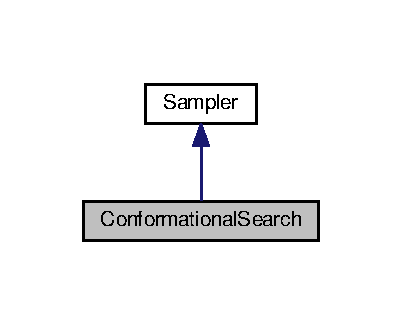
\includegraphics[width=193pt]{classConformationalSearch__inherit__graph}
\end{center}
\end{figure}


Collaboration diagram for Conformational\+Search\+:\nopagebreak
\begin{figure}[H]
\begin{center}
\leavevmode
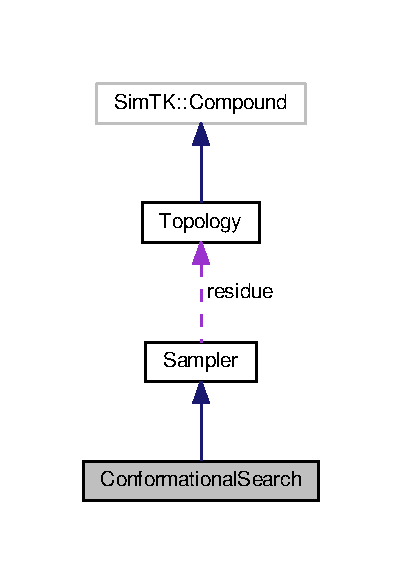
\includegraphics[width=193pt]{classConformationalSearch__coll__graph}
\end{center}
\end{figure}
\subsection*{Public Member Functions}
\begin{DoxyCompactItemize}
\item 
{\bfseries Conformational\+Search} (Sim\+T\+K\+::\+Compound\+System $\ast$arg\+Compound\+System, Sim\+T\+K\+::\+Simbody\+Matter\+Subsystem $\ast$arg\+Matter, std\+::vector$<$ \hyperlink{classTopology}{Topology} $\ast$ $>$ \&topologies, Sim\+T\+K\+::\+Du\+M\+M\+Force\+Field\+Subsystem $\ast$arg\+Dumm, Sim\+T\+K\+::\+General\+Force\+Subsystem $\ast$forces, Sim\+T\+K\+::\+Time\+Stepper $\ast$arg\+Time\+Stepper)\hypertarget{classConformationalSearch_a30d5c83ad10a93526cd286bbea9d81e0}{}\label{classConformationalSearch_a30d5c83ad10a93526cd286bbea9d81e0}

\item 
Sim\+T\+K\+::\+Real {\bfseries get\+Temperature} (void)\hypertarget{classConformationalSearch_a680403e9df0f184e0ff8cc2bd6101326}{}\label{classConformationalSearch_a680403e9df0f184e0ff8cc2bd6101326}

\item 
void {\bfseries set\+Temperature} (Sim\+T\+K\+::\+Real)\hypertarget{classConformationalSearch_a460af75a5e3dbbdb979ad7b0a1cd90c4}{}\label{classConformationalSearch_a460af75a5e3dbbdb979ad7b0a1cd90c4}

\item 
void {\bfseries set\+Thermostat} (Thermostat\+Name)\hypertarget{classConformationalSearch_a56af33f8eefcf1ea424cf5681e72f972}{}\label{classConformationalSearch_a56af33f8eefcf1ea424cf5681e72f972}

\item 
void {\bfseries set\+Thermostat} (std\+::string)\hypertarget{classConformationalSearch_ab702f7fc2db2202aef6f51c27a9ae0e2}{}\label{classConformationalSearch_ab702f7fc2db2202aef6f51c27a9ae0e2}

\item 
void {\bfseries set\+Thermostat} (const char $\ast$)\hypertarget{classConformationalSearch_a263ce928f1e8ba4d51175f57655321fa}{}\label{classConformationalSearch_a263ce928f1e8ba4d51175f57655321fa}

\item 
virtual Thermostat\+Name {\bfseries get\+Thermostat} (void)\hypertarget{classConformationalSearch_a4734babe9b91d622e32ce2974ccf205b}{}\label{classConformationalSearch_a4734babe9b91d622e32ce2974ccf205b}

\item 
virtual void \hyperlink{classConformationalSearch_af7bf3e9bf537c6636d51fab224ec73d4}{initialize} (Sim\+T\+K\+::\+State \&advanced, Sim\+T\+K\+::\+Real arg\+Temperature, bool arg\+Use\+Fixman=true)
\item 
virtual void \hyperlink{classConformationalSearch_ac9c0b36dfb58b98e376ebbda2fc4bf25}{reinitialize} (Sim\+T\+K\+::\+State \&advanced, Sim\+T\+K\+::\+Real arg\+Temperature)
\item 
void {\bfseries set\+Set\+T\+Vector} (const Sim\+T\+K\+::\+State \&advanced)\hypertarget{classConformationalSearch_a97d594ce806a003f606a78c0fcb49683}{}\label{classConformationalSearch_a97d594ce806a003f606a78c0fcb49683}

\item 
Sim\+T\+K\+::\+Transform $\ast$ {\bfseries get\+Set\+T\+Vector} (void)\hypertarget{classConformationalSearch_a563043f252dcbc1cd27599df7d4dd667}{}\label{classConformationalSearch_a563043f252dcbc1cd27599df7d4dd667}

\item 
void {\bfseries assign\+Conf\+From\+Set\+T\+Vector} (Sim\+T\+K\+::\+State \&advanced)\hypertarget{classConformationalSearch_a83b143b3f3cbc45455c7119767e42f18}{}\label{classConformationalSearch_a83b143b3f3cbc45455c7119767e42f18}

\item 
void {\bfseries set\+T\+Vector} (const Sim\+T\+K\+::\+State \&advanced)\hypertarget{classConformationalSearch_ae7d8679e15ae2b564c56aff7d387e686}{}\label{classConformationalSearch_ae7d8679e15ae2b564c56aff7d387e686}

\item 
void {\bfseries set\+T\+Vector} (Sim\+T\+K\+::\+Transform $\ast$)\hypertarget{classConformationalSearch_ad09b271bc41b4cac94ffcbf253b5afd0}{}\label{classConformationalSearch_ad09b271bc41b4cac94ffcbf253b5afd0}

\item 
Sim\+T\+K\+::\+Transform $\ast$ {\bfseries get\+T\+Vector} (void)\hypertarget{classConformationalSearch_abc47122d4b73e960debbb5902157a299}{}\label{classConformationalSearch_abc47122d4b73e960debbb5902157a299}

\item 
void {\bfseries assign\+Conf\+From\+T\+Vector} (Sim\+T\+K\+::\+State \&advanced)\hypertarget{classConformationalSearch_ab9b4f70f4a4f826a430461403f2d427a}{}\label{classConformationalSearch_ab9b4f70f4a4f826a430461403f2d427a}

\item 
void \hyperlink{classConformationalSearch_a1656b70ede0f43765c9379737d6e6697}{propose} (Sim\+T\+K\+::\+State \&advanced)
\item 
Sim\+T\+K\+::\+Real {\bfseries get\+Set\+PE} (void)\hypertarget{classConformationalSearch_a031616fd5832b60edbb22bc77edeed3d}{}\label{classConformationalSearch_a031616fd5832b60edbb22bc77edeed3d}

\item 
void {\bfseries set\+Set\+PE} (Sim\+T\+K\+::\+Real arg\+PE)\hypertarget{classConformationalSearch_a9e5a5be6a8146f1ea65e4f59495e1dca}{}\label{classConformationalSearch_a9e5a5be6a8146f1ea65e4f59495e1dca}

\item 
Sim\+T\+K\+::\+Real {\bfseries get\+Old\+PE} (void)\hypertarget{classConformationalSearch_a4863b464944280a40272a50ff87ec86f}{}\label{classConformationalSearch_a4863b464944280a40272a50ff87ec86f}

\item 
void {\bfseries set\+Old\+PE} (Sim\+T\+K\+::\+Real arg\+PE)\hypertarget{classConformationalSearch_a80338d2d1862f2d54ccba4fb71cf8d31}{}\label{classConformationalSearch_a80338d2d1862f2d54ccba4fb71cf8d31}

\item 
void {\bfseries set\+Set\+Fixman} (Sim\+T\+K\+::\+Real)\hypertarget{classConformationalSearch_ae2ad62d8cc4a95c0a64acd989e96ca1b}{}\label{classConformationalSearch_ae2ad62d8cc4a95c0a64acd989e96ca1b}

\item 
Sim\+T\+K\+::\+Real {\bfseries get\+Set\+Fixman} (void)\hypertarget{classConformationalSearch_a89f080301b7c62aa1670d5aaa62cda64}{}\label{classConformationalSearch_a89f080301b7c62aa1670d5aaa62cda64}

\item 
void {\bfseries set\+R\+EP} (Sim\+T\+K\+::\+Real)\hypertarget{classConformationalSearch_ae6ee4184dd53516e76a8702c19d613db}{}\label{classConformationalSearch_ae6ee4184dd53516e76a8702c19d613db}

\item 
Sim\+T\+K\+::\+Real {\bfseries get\+R\+EP} (void)\hypertarget{classConformationalSearch_a07c19a37a7842e46d1de3ed3ede0406c}{}\label{classConformationalSearch_a07c19a37a7842e46d1de3ed3ede0406c}

\item 
void {\bfseries set\+Old\+Fixman} (Sim\+T\+K\+::\+Real)\hypertarget{classConformationalSearch_a92745f4bb8f9bcfce042d8f7fe9685dc}{}\label{classConformationalSearch_a92745f4bb8f9bcfce042d8f7fe9685dc}

\item 
Sim\+T\+K\+::\+Real {\bfseries get\+Old\+Fixman} (void)\hypertarget{classConformationalSearch_a0adc7a570887d26e4ac723fe6273ee7c}{}\label{classConformationalSearch_a0adc7a570887d26e4ac723fe6273ee7c}

\item 
Sim\+T\+K\+::\+Real {\bfseries get\+P\+E\+From\+Evaluator} (Sim\+T\+K\+::\+State \&some\+State)\hypertarget{classConformationalSearch_a9cd1201735ce2d42c355d46653336730}{}\label{classConformationalSearch_a9cd1201735ce2d42c355d46653336730}

\item 
void {\bfseries use\+Fixman\+Potential} (void)\hypertarget{classConformationalSearch_ad1602c7b9f5798a10014891e16f92e55}{}\label{classConformationalSearch_ad1602c7b9f5798a10014891e16f92e55}

\item 
bool {\bfseries is\+Using\+Fixman\+Potential} (void)\hypertarget{classConformationalSearch_a5196d77103c8ebddf76cf20d80776678}{}\label{classConformationalSearch_a5196d77103c8ebddf76cf20d80776678}

\item 
Sim\+T\+K\+::\+Real {\bfseries calc\+Fixman} (Sim\+T\+K\+::\+State \&some\+State)\hypertarget{classConformationalSearch_ad5bd251a7c87f4fe14902623cfb563cb}{}\label{classConformationalSearch_ad5bd251a7c87f4fe14902623cfb563cb}

\item 
Sim\+T\+K\+::\+Real {\bfseries calc\+Num\+Fixman} (Sim\+T\+K\+::\+State \&some\+State)\hypertarget{classConformationalSearch_ad37a01bf90ff5ddf057304d85db10f84}{}\label{classConformationalSearch_ad37a01bf90ff5ddf057304d85db10f84}

\item 
Sim\+T\+K\+::\+Real {\bfseries calc\+Num\+DetM} (Sim\+T\+K\+::\+State \&some\+State)\hypertarget{classConformationalSearch_ae588524a66f8c60ec2f9a3d64c25d478}{}\label{classConformationalSearch_ae588524a66f8c60ec2f9a3d64c25d478}

\item 
void {\bfseries send\+Conf\+To\+Evaluator} (void)\hypertarget{classConformationalSearch_a2f99ba20e4ddaba8cc93d3d767635f27}{}\label{classConformationalSearch_a2f99ba20e4ddaba8cc93d3d767635f27}

\item 
bool {\bfseries get\+Always\+Accept} (void)\hypertarget{classConformationalSearch_a05b4f8ae8a164278377351aeedac5150}{}\label{classConformationalSearch_a05b4f8ae8a164278377351aeedac5150}

\item 
void {\bfseries set\+Always\+Accept} (bool)\hypertarget{classConformationalSearch_a7ac67acfed3ab31bda075427ec86ae09}{}\label{classConformationalSearch_a7ac67acfed3ab31bda075427ec86ae09}

\item 
void {\bfseries update} (Sim\+T\+K\+::\+State \&)\hypertarget{classConformationalSearch_a0c5d9660ec343bd9e6910f6498375cc3}{}\label{classConformationalSearch_a0c5d9660ec343bd9e6910f6498375cc3}

\item 
int {\bfseries get\+Accepted\+Steps} (void)\hypertarget{classConformationalSearch_ac15a62651e9928188b2f617b742284e4}{}\label{classConformationalSearch_ac15a62651e9928188b2f617b742284e4}

\end{DoxyCompactItemize}
\subsection*{Protected Attributes}
\begin{DoxyCompactItemize}
\item 
std\+::vector$<$ Sim\+T\+K\+::\+Transform $>$ {\bfseries Set\+T\+Vector}\hypertarget{classConformationalSearch_ab57c3b196616d1c49daf7fc95c87368e}{}\label{classConformationalSearch_ab57c3b196616d1c49daf7fc95c87368e}

\item 
std\+::vector$<$ Sim\+T\+K\+::\+Transform $>$ {\bfseries T\+Vector}\hypertarget{classConformationalSearch_aa65667a9158bf2dbbc5ed86167b9da21}{}\label{classConformationalSearch_aa65667a9158bf2dbbc5ed86167b9da21}

\item 
Sim\+T\+K\+::\+Real {\bfseries pe\+\_\+set}\hypertarget{classConformationalSearch_a124556d6acdd92a7f47b6655c696358f}{}\label{classConformationalSearch_a124556d6acdd92a7f47b6655c696358f}

\item 
Sim\+T\+K\+::\+Real {\bfseries pe\+\_\+o}\hypertarget{classConformationalSearch_a4225545cc7f1246b0ef8fab3a8221a37}{}\label{classConformationalSearch_a4225545cc7f1246b0ef8fab3a8221a37}

\item 
Sim\+T\+K\+::\+Real {\bfseries temperature}\hypertarget{classConformationalSearch_a88f50b05630ba9f65567fa2b1e709108}{}\label{classConformationalSearch_a88f50b05630ba9f65567fa2b1e709108}

\item 
Sim\+T\+K\+::\+Real {\bfseries RT}\hypertarget{classConformationalSearch_ae44e6a0fb042897741b587ac2b400046}{}\label{classConformationalSearch_ae44e6a0fb042897741b587ac2b400046}

\item 
bool {\bfseries use\+Fixman} = false\hypertarget{classConformationalSearch_ae9286f4596daf45d023670c0b6d0da2d}{}\label{classConformationalSearch_ae9286f4596daf45d023670c0b6d0da2d}

\item 
bool {\bfseries always\+Accept} = false\hypertarget{classConformationalSearch_a095f59dd63f97355f707b8a06b7ffb2b}{}\label{classConformationalSearch_a095f59dd63f97355f707b8a06b7ffb2b}

\item 
Sim\+T\+K\+::\+Real {\bfseries fix\+\_\+set}\hypertarget{classConformationalSearch_a07418527706294a33e21a71f6b21eee1}{}\label{classConformationalSearch_a07418527706294a33e21a71f6b21eee1}

\item 
Sim\+T\+K\+::\+Real {\bfseries fix\+\_\+o}\hypertarget{classConformationalSearch_a289685f1a0f36f488310c0d3e5cf9dde}{}\label{classConformationalSearch_a289685f1a0f36f488310c0d3e5cf9dde}

\item 
Sim\+T\+K\+::\+Real {\bfseries fix\+\_\+n}\hypertarget{classConformationalSearch_ac4d43982963f73d8ecfeba740428b4b8}{}\label{classConformationalSearch_ac4d43982963f73d8ecfeba740428b4b8}

\item 
Sim\+T\+K\+::\+Real {\bfseries residual\+Embedded\+Potential} = 0.\+0\hypertarget{classConformationalSearch_a7a7592e9f594d36951150ddf0e640421}{}\label{classConformationalSearch_a7a7592e9f594d36951150ddf0e640421}

\item 
int {\bfseries accepted\+Steps} = 0\hypertarget{classConformationalSearch_aeb36f99ac50811075662bfa812323c59}{}\label{classConformationalSearch_aeb36f99ac50811075662bfa812323c59}

\item 
boost\+::random\+::mt19937 {\bfseries random\+Engine} = boost\+::random\+::mt19937()\hypertarget{classConformationalSearch_a04f9202eee8064ffa5671765c028cb4d}{}\label{classConformationalSearch_a04f9202eee8064ffa5671765c028cb4d}

\item 
boost\+::random\+::uniform\+\_\+real\+\_\+distribution$<$ double $>$ {\bfseries uniform\+Real\+Distribution\+\_\+0\+\_\+2pi}
\item 
boost\+::random\+::uniform\+\_\+real\+\_\+distribution$<$ double $>$ {\bfseries uniform\+Real\+Distribution\+\_\+mpi\+\_\+pi}
\item 
boost\+::random\+::uniform\+\_\+real\+\_\+distribution$<$ double $>$ {\bfseries uniform\+Real\+Distribution}
\item 
boost\+::random\+::uniform\+\_\+real\+\_\+distribution$<$ double $>$ {\bfseries uniform\+Real\+Distribution\+\_\+m1\+\_\+1}
\item 
boost\+::normal\+\_\+distribution {\bfseries gaurand} = boost\+::normal\+\_\+distribution$<$$>$(0.\+0, 1.\+0)\hypertarget{classConformationalSearch_ad7edb7b4f9b9c8d3022dc2e73f276435}{}\label{classConformationalSearch_ad7edb7b4f9b9c8d3022dc2e73f276435}

\end{DoxyCompactItemize}
\subsection*{Additional Inherited Members}


\subsection{Member Function Documentation}
\index{Conformational\+Search@{Conformational\+Search}!initialize@{initialize}}
\index{initialize@{initialize}!Conformational\+Search@{Conformational\+Search}}
\subsubsection[{\texorpdfstring{initialize(\+Sim\+T\+K\+::\+State \&advanced, Sim\+T\+K\+::\+Real arg\+Temperature, bool arg\+Use\+Fixman=true)}{initialize(SimTK::State &advanced, SimTK::Real argTemperature, bool argUseFixman=true)}}]{\setlength{\rightskip}{0pt plus 5cm}void Conformational\+Search\+::initialize (
\begin{DoxyParamCaption}
\item[{Sim\+T\+K\+::\+State \&}]{advanced, }
\item[{Sim\+T\+K\+::\+Real}]{arg\+Temperature, }
\item[{bool}]{arg\+Use\+Fixman = {\ttfamily true}}
\end{DoxyParamCaption}
)\hspace{0.3cm}{\ttfamily [virtual]}}\hypertarget{classConformationalSearch_af7bf3e9bf537c6636d51fab224ec73d4}{}\label{classConformationalSearch_af7bf3e9bf537c6636d51fab224ec73d4}
Seed the random number generator. Set simulation temperature, variables that store the configuration and variables that store the energies, both needed for the acception-\/rejection step. Also realize velocities and initialize the timestepper. \index{Conformational\+Search@{Conformational\+Search}!propose@{propose}}
\index{propose@{propose}!Conformational\+Search@{Conformational\+Search}}
\subsubsection[{\texorpdfstring{propose(\+Sim\+T\+K\+::\+State \&advanced)}{propose(SimTK::State &advanced)}}]{\setlength{\rightskip}{0pt plus 5cm}void Conformational\+Search\+::propose (
\begin{DoxyParamCaption}
\item[{Sim\+T\+K\+::\+State \&}]{some\+State}
\end{DoxyParamCaption}
)\hspace{0.3cm}{\ttfamily [virtual]}}\hypertarget{classConformationalSearch_a1656b70ede0f43765c9379737d6e6697}{}\label{classConformationalSearch_a1656b70ede0f43765c9379737d6e6697}
Propose a move 

Implements \hyperlink{classSampler_a3022d2efacf6107b3fba506d31e2919e}{Sampler}.

\index{Conformational\+Search@{Conformational\+Search}!reinitialize@{reinitialize}}
\index{reinitialize@{reinitialize}!Conformational\+Search@{Conformational\+Search}}
\subsubsection[{\texorpdfstring{reinitialize(\+Sim\+T\+K\+::\+State \&advanced, Sim\+T\+K\+::\+Real arg\+Temperature)}{reinitialize(SimTK::State &advanced, SimTK::Real argTemperature)}}]{\setlength{\rightskip}{0pt plus 5cm}void Conformational\+Search\+::reinitialize (
\begin{DoxyParamCaption}
\item[{Sim\+T\+K\+::\+State \&}]{advanced, }
\item[{Sim\+T\+K\+::\+Real}]{arg\+Temperature}
\end{DoxyParamCaption}
)\hspace{0.3cm}{\ttfamily [virtual]}}\hypertarget{classConformationalSearch_ac9c0b36dfb58b98e376ebbda2fc4bf25}{}\label{classConformationalSearch_ac9c0b36dfb58b98e376ebbda2fc4bf25}
Same as initialize 

\subsection{Member Data Documentation}
\index{Conformational\+Search@{Conformational\+Search}!uniform\+Real\+Distribution@{uniform\+Real\+Distribution}}
\index{uniform\+Real\+Distribution@{uniform\+Real\+Distribution}!Conformational\+Search@{Conformational\+Search}}
\subsubsection[{\texorpdfstring{uniform\+Real\+Distribution}{uniformRealDistribution}}]{\setlength{\rightskip}{0pt plus 5cm}boost\+::random\+::uniform\+\_\+real\+\_\+distribution$<$double$>$ Conformational\+Search\+::uniform\+Real\+Distribution\hspace{0.3cm}{\ttfamily [protected]}}\hypertarget{classConformationalSearch_a9a50545b5c5401f06013143a91b46340}{}\label{classConformationalSearch_a9a50545b5c5401f06013143a91b46340}
{\bfseries Initial value\+:}
\begin{DoxyCode}
=
        boost::random::uniform\_real\_distribution<double>(SimTK::Zero, SimTK::One)
\end{DoxyCode}
\index{Conformational\+Search@{Conformational\+Search}!uniform\+Real\+Distribution\+\_\+0\+\_\+2pi@{uniform\+Real\+Distribution\+\_\+0\+\_\+2pi}}
\index{uniform\+Real\+Distribution\+\_\+0\+\_\+2pi@{uniform\+Real\+Distribution\+\_\+0\+\_\+2pi}!Conformational\+Search@{Conformational\+Search}}
\subsubsection[{\texorpdfstring{uniform\+Real\+Distribution\+\_\+0\+\_\+2pi}{uniformRealDistribution_0_2pi}}]{\setlength{\rightskip}{0pt plus 5cm}boost\+::random\+::uniform\+\_\+real\+\_\+distribution$<$double$>$ Conformational\+Search\+::uniform\+Real\+Distribution\+\_\+0\+\_\+2pi\hspace{0.3cm}{\ttfamily [protected]}}\hypertarget{classConformationalSearch_a655470c22c0772aaba13d2a707892034}{}\label{classConformationalSearch_a655470c22c0772aaba13d2a707892034}
{\bfseries Initial value\+:}
\begin{DoxyCode}
=
        boost::random::uniform\_real\_distribution<double>(SimTK::Zero, 2*SimTK::Pi)
\end{DoxyCode}
\index{Conformational\+Search@{Conformational\+Search}!uniform\+Real\+Distribution\+\_\+m1\+\_\+1@{uniform\+Real\+Distribution\+\_\+m1\+\_\+1}}
\index{uniform\+Real\+Distribution\+\_\+m1\+\_\+1@{uniform\+Real\+Distribution\+\_\+m1\+\_\+1}!Conformational\+Search@{Conformational\+Search}}
\subsubsection[{\texorpdfstring{uniform\+Real\+Distribution\+\_\+m1\+\_\+1}{uniformRealDistribution_m1_1}}]{\setlength{\rightskip}{0pt plus 5cm}boost\+::random\+::uniform\+\_\+real\+\_\+distribution$<$double$>$ Conformational\+Search\+::uniform\+Real\+Distribution\+\_\+m1\+\_\+1\hspace{0.3cm}{\ttfamily [protected]}}\hypertarget{classConformationalSearch_a28866d2f85e7abaa8715dfcd72f8dd2c}{}\label{classConformationalSearch_a28866d2f85e7abaa8715dfcd72f8dd2c}
{\bfseries Initial value\+:}
\begin{DoxyCode}
=
        boost::random::uniform\_real\_distribution<double>((-1)*SimTK::One, SimTK::One)
\end{DoxyCode}
\index{Conformational\+Search@{Conformational\+Search}!uniform\+Real\+Distribution\+\_\+mpi\+\_\+pi@{uniform\+Real\+Distribution\+\_\+mpi\+\_\+pi}}
\index{uniform\+Real\+Distribution\+\_\+mpi\+\_\+pi@{uniform\+Real\+Distribution\+\_\+mpi\+\_\+pi}!Conformational\+Search@{Conformational\+Search}}
\subsubsection[{\texorpdfstring{uniform\+Real\+Distribution\+\_\+mpi\+\_\+pi}{uniformRealDistribution_mpi_pi}}]{\setlength{\rightskip}{0pt plus 5cm}boost\+::random\+::uniform\+\_\+real\+\_\+distribution$<$double$>$ Conformational\+Search\+::uniform\+Real\+Distribution\+\_\+mpi\+\_\+pi\hspace{0.3cm}{\ttfamily [protected]}}\hypertarget{classConformationalSearch_a0d6e470379038b622a72cde9be8749f3}{}\label{classConformationalSearch_a0d6e470379038b622a72cde9be8749f3}
{\bfseries Initial value\+:}
\begin{DoxyCode}
=
        boost::random::uniform\_real\_distribution<double>((-1)*SimTK::Pi, SimTK::Pi)
\end{DoxyCode}


The documentation for this class was generated from the following files\+:\begin{DoxyCompactItemize}
\item 
include/gmolmodel/Conformational\+Search.\+hpp\item 
src/\hyperlink{ConformationalSearch_8cpp}{Conformational\+Search.\+cpp}\end{DoxyCompactItemize}

\hypertarget{classContext}{}\section{Context Class Reference}
\label{classContext}\index{Context@{Context}}
\subsection*{Public Member Functions}
\begin{DoxyCompactItemize}
\item 
{\bfseries Context} (const \hyperlink{classSetupReader}{Setup\+Reader} \&setup\+Reader, \hyperlink{classWorld}{World} $\ast$, std\+::string log\+Filename\+Arg)\hypertarget{classContext_a6e4e9c4b84131ee9444c09898a35ebb5}{}\label{classContext_a6e4e9c4b84131ee9444c09898a35ebb5}

\item 
{\bfseries Context} (const \hyperlink{classSetupReader}{Setup\+Reader} \&setup\+Reader, std\+::string log\+Filename\+Arg)\hypertarget{classContext_a86b58f3d114611bae1adca9ef994e635}{}\label{classContext_a86b58f3d114611bae1adca9ef994e635}

\item 
\hyperlink{classWorld}{World} $\ast$ {\bfseries Add\+World} (bool visual, Sim\+T\+K\+::\+Real visualizer\+Frequency=0.\+0015)\hypertarget{classContext_a26871eab3b4d582d71946f71f0e41e2d}{}\label{classContext_a26871eab3b4d582d71946f71f0e41e2d}

\item 
\hyperlink{classWorld}{World} $\ast$ {\bfseries get\+World} () const \hypertarget{classContext_aaa4a6f192a80b8c95fb3c8ed2b7089e6}{}\label{classContext_aaa4a6f192a80b8c95fb3c8ed2b7089e6}

\item 
\hyperlink{classWorld}{World} $\ast$ {\bfseries get\+World} (int which) const \hypertarget{classContext_a59ef49f3ad910f73bf7101a85b30208f}{}\label{classContext_a59ef49f3ad910f73bf7101a85b30208f}

\item 
\hyperlink{classWorld}{World} $\ast$ {\bfseries upd\+World} ()\hypertarget{classContext_a66e0ae4f45acca7572f2f9009c24acc7}{}\label{classContext_a66e0ae4f45acca7572f2f9009c24acc7}

\item 
\hyperlink{classWorld}{World} $\ast$ {\bfseries upd\+World} (int which)\hypertarget{classContext_afc4d3df76061253608081ba831940647}{}\label{classContext_afc4d3df76061253608081ba831940647}

\item 
unsigned int {\bfseries get\+Nof\+Worlds} ()\hypertarget{classContext_ac31e1ba0186a5b6a7d4ade15958cb2eb}{}\label{classContext_ac31e1ba0186a5b6a7d4ade15958cb2eb}

\item 
Sim\+T\+K\+::\+Du\+M\+M\+Force\+Field\+Subsystem $\ast$ {\bfseries upd\+Force\+Field} (int which\+World)\hypertarget{classContext_af1048e799296dee3b63b93ae79dbc4ff}{}\label{classContext_af1048e799296dee3b63b93ae79dbc4ff}

\item 
Sim\+T\+K\+::\+State \& {\bfseries upd\+Advanced\+State} (int which\+World, int which\+Sampler)\hypertarget{classContext_aba3acd8e9749a3b4d8ad5be5876acf08}{}\label{classContext_aba3acd8e9749a3b4d8ad5be5876acf08}

\item 
bool {\bfseries load\+Topology\+File} (int which\+World, int which\+Molecule, std\+::string topology\+Filename)\hypertarget{classContext_accc36f76330e7dcc5ecb29a91b5f51e3}{}\label{classContext_accc36f76330e7dcc5ecb29a91b5f51e3}

\item 
bool {\bfseries load\+Coordinates\+File} (int which\+World, int which\+Molecule, std\+::string coordinates\+Filename)\hypertarget{classContext_aef08b71378a98d420be726c420c15dcb}{}\label{classContext_aef08b71378a98d420be726c420c15dcb}

\item 
bool {\bfseries load\+Rigid\+Bodies\+Specs} (int which\+World, int which\+Molecule, std\+::string R\+B\+Specs\+FN)\hypertarget{classContext_aa0e54a21febcfd4614ac53a85a5af690}{}\label{classContext_aa0e54a21febcfd4614ac53a85a5af690}

\item 
bool {\bfseries load\+Flexible\+Bonds\+Specs} (int which\+World, int which\+Molecule, std\+::string Flex\+Specs\+FN)\hypertarget{classContext_a398bc5df5ca7229ad4351eb88d08c9db}{}\label{classContext_a398bc5df5ca7229ad4351eb88d08c9db}

\item 
void {\bfseries set\+Regimen} (int which\+World, int which\+Molecule, std\+::string regimen)\hypertarget{classContext_a3dd54f31104323e4d8df399da85e8ce1}{}\label{classContext_a3dd54f31104323e4d8df399da85e8ce1}

\item 
void \hyperlink{classContext_a35136bab91fe9f196a676a345b404339}{Add\+Molecules} (std\+::vector$<$ std\+::string $>$ arg\+Roots)
\item 
void {\bfseries model\+Topologies} (std\+::vector$<$ std\+::string $>$ Ground\+To\+Compound\+Mobilizer\+Types)\hypertarget{classContext_acf571a7ef2864aa092d411c0dfb8658a}{}\label{classContext_acf571a7ef2864aa092d411c0dfb8658a}

\item 
void {\bfseries realize\+Topology} ()\hypertarget{classContext_a713fd59ba4a18056e3b359d1c8a669e0}{}\label{classContext_a713fd59ba4a18056e3b359d1c8a669e0}

\item 
void {\bfseries Load\+Worlds\+From\+Setup} (\hyperlink{classSetupReader}{Setup\+Reader} \&)\hypertarget{classContext_a7a7e949c06bc4eaec17f532ef6d58158}{}\label{classContext_a7a7e949c06bc4eaec17f532ef6d58158}

\item 
int {\bfseries get\+Nof\+Molecules} ()\hypertarget{classContext_ac55253cfbdd83b5966c7ee38494fea9c}{}\label{classContext_ac55253cfbdd83b5966c7ee38494fea9c}

\item 
void {\bfseries set\+Vdw\+Mixing\+Rule} (Sim\+T\+K\+::\+Du\+M\+M\+Force\+Field\+Subsystem\+::\+Vdw\+Mixing\+Rule mixing\+Rule)\hypertarget{classContext_a5f797c56bf76df0f1f943737071c4d95}{}\label{classContext_a5f797c56bf76df0f1f943737071c4d95}

\item 
float {\bfseries get\+Temperature} (int which\+World)\hypertarget{classContext_ae59336ed3797d3efac98d0142d1dc79c}{}\label{classContext_ae59336ed3797d3efac98d0142d1dc79c}

\item 
void {\bfseries set\+Temperature} (int which\+World, float some\+Temperature)\hypertarget{classContext_a5bcedc50b4316f5b47ec0fee42daeeab}{}\label{classContext_a5bcedc50b4316f5b47ec0fee42daeeab}

\item 
float {\bfseries get\+Guidance\+Temperature} (int which\+World, int which\+Sampler)\hypertarget{classContext_aa304e434bf030976e7075ffe040ee949}{}\label{classContext_aa304e434bf030976e7075ffe040ee949}

\item 
void {\bfseries set\+Guidance\+Temperature} (int which\+World, int which\+Sampler, float some\+Temperature)\hypertarget{classContext_ada1e12614883a246b745bb650fce2bec}{}\label{classContext_ada1e12614883a246b745bb650fce2bec}

\item 
Base\+Sampler $\ast$ {\bfseries add\+Sampler} (int which\+World, Sampler\+Name which\+Sampler)\hypertarget{classContext_a561523aef8ecc0f49fa903c291b51213}{}\label{classContext_a561523aef8ecc0f49fa903c291b51213}

\item 
void {\bfseries initialize\+Sampler} (int which\+World, int which\+Sampler)\hypertarget{classContext_a7a019024e7574751c77df9b0229ebae8}{}\label{classContext_a7a019024e7574751c77df9b0229ebae8}

\item 
void {\bfseries set\+Amber\+Force\+Field\+Scale\+Factors} (int which\+World)\hypertarget{classContext_a6005c1dea1595627cf11a72d9fbe5178}{}\label{classContext_a6005c1dea1595627cf11a72d9fbe5178}

\item 
void {\bfseries set\+Global\+Force\+Field\+Scale\+Factor} (int which\+World, Sim\+T\+K\+::\+Real)\hypertarget{classContext_ab6bcb997cdd1aec798d9018692afcd27}{}\label{classContext_ab6bcb997cdd1aec798d9018692afcd27}

\item 
void {\bfseries set\+Gbsa\+Global\+Scale\+Factor} (int which\+World, Sim\+T\+K\+::\+Real)\hypertarget{classContext_aa1d216cc40b9dcfde36652a965e56f05}{}\label{classContext_aa1d216cc40b9dcfde36652a965e56f05}

\item 
int {\bfseries get\+Nof\+M\+D\+Steps\+Per\+Sample} (int which\+World, int which\+Sampler)\hypertarget{classContext_aed9b2985cdc6ae1201f0c4b473c6c0e0}{}\label{classContext_aed9b2985cdc6ae1201f0c4b473c6c0e0}

\item 
void {\bfseries set\+Nof\+M\+D\+Steps\+Per\+Sample} (int which\+World, int which\+Sampler, int M\+D\+Steps\+Per\+Sample)\hypertarget{classContext_a3fd9b856887ed4e85ab79c9dfc18220f}{}\label{classContext_a3fd9b856887ed4e85ab79c9dfc18220f}

\item 
const float {\bfseries get\+Timestep} (int which\+World, int which\+Sampler)\hypertarget{classContext_ad21f2aaeda92692ef1b33e974ff85295}{}\label{classContext_ad21f2aaeda92692ef1b33e974ff85295}

\item 
void {\bfseries set\+Timestep} (int which\+World, int which\+Sampler, float time\+Step)\hypertarget{classContext_a82b6fd848de84eaa1a214016cc171942}{}\label{classContext_a82b6fd848de84eaa1a214016cc171942}

\item 
void {\bfseries use\+Fixman\+Potential} (int which\+World, int which\+Sampler)\hypertarget{classContext_ac6eceed7cf476ec4dd14755bc39f0561}{}\label{classContext_ac6eceed7cf476ec4dd14755bc39f0561}

\item 
bool {\bfseries is\+Using\+Fixman\+Potential} (int which\+World, int which\+Sampler)\hypertarget{classContext_a41b54fb16e7028c4c4c1a9502d19a2fd}{}\label{classContext_a41b54fb16e7028c4c4c1a9502d19a2fd}

\item 
void {\bfseries add\+Fixman\+Torque} (int which\+World)\hypertarget{classContext_a18cb34cca0c2b7934b9bd1170ddbd9d8}{}\label{classContext_a18cb34cca0c2b7934b9bd1170ddbd9d8}

\item 
bool {\bfseries is\+Using\+Fixman\+Torque} (int which\+World)\hypertarget{classContext_aaba8608b9266c8251019e2204b5d5f05}{}\label{classContext_aaba8608b9266c8251019e2204b5d5f05}

\item 
void {\bfseries set\+Fixman\+Torque\+Scale\+Factor} (int which\+World, double scale\+Factor)\hypertarget{classContext_af69b67139cca2e43cf3af0cc8114d8ea}{}\label{classContext_af69b67139cca2e43cf3af0cc8114d8ea}

\item 
void {\bfseries set\+Fixman\+Torque\+Temperature} (int which\+World, double temperature)\hypertarget{classContext_aa3cba363a73461a76cb9112b3868337d}{}\label{classContext_aa3cba363a73461a76cb9112b3868337d}

\item 
int {\bfseries get\+Nof\+Rounds} ()\hypertarget{classContext_afbc7cfc13d3d0f5780b7876216b8194f}{}\label{classContext_afbc7cfc13d3d0f5780b7876216b8194f}

\item 
void {\bfseries set\+Nof\+Rounds} (int nof\+Rounds)\hypertarget{classContext_a33526796ba166e7a7975956ad8ff0482}{}\label{classContext_a33526796ba166e7a7975956ad8ff0482}

\item 
int {\bfseries get\+Nof\+Samples\+Per\+Round} (int which\+World)\hypertarget{classContext_aad374e89822a443141d992b986ede2fe}{}\label{classContext_aad374e89822a443141d992b986ede2fe}

\item 
void {\bfseries set\+Nof\+Samples\+Per\+Round} (int which\+World, int M\+C\+Steps\+Per\+Round)\hypertarget{classContext_a1097bde655d6678da5a79f30ebbff621}{}\label{classContext_a1097bde655d6678da5a79f30ebbff621}

\item 
int {\bfseries get\+World\+Index} (int which)\hypertarget{classContext_a3dde15772536cf1d92da67b9bc7c9f9c}{}\label{classContext_a3dde15772536cf1d92da67b9bc7c9f9c}

\item 
void {\bfseries initialize\+Mixing\+Paramters} ()\hypertarget{classContext_aa5ce3f96fd7a71a4ea55599b1e4cbb16}{}\label{classContext_aa5ce3f96fd7a71a4ea55599b1e4cbb16}

\item 
void {\bfseries Rotate\+Worlds} ()\hypertarget{classContext_a4b30d57929b8019f0f80c4a5711f8766}{}\label{classContext_a4b30d57929b8019f0f80c4a5711f8766}

\item 
void {\bfseries Run} (\hyperlink{classSetupReader}{Setup\+Reader} \&)\hypertarget{classContext_a5aa7b7c23dba333d40f41b7951dbb175}{}\label{classContext_a5aa7b7c23dba333d40f41b7951dbb175}

\item 
void {\bfseries Run} (int how\+Many\+Rounds, float Ti, float Tf, bool is\+World\+Order\+Random)\hypertarget{classContext_a7348fe547472332d18426af129b9a3a4}{}\label{classContext_a7348fe547472332d18426af129b9a3a4}

\item 
void {\bfseries Run\+Simulated\+Tempering} (int how\+Many\+Rounds, float Ti, float Tf)\hypertarget{classContext_aeb6a4048885ad4003ac94474d0b30df1}{}\label{classContext_aeb6a4048885ad4003ac94474d0b30df1}

\item 
void {\bfseries set\+Nof\+Boost\+Stairs} (int which\+World, int how\+Many\+Stairs)\hypertarget{classContext_a3fd7bc68f83c99de8efde6959df55a19}{}\label{classContext_a3fd7bc68f83c99de8efde6959df55a19}

\item 
int {\bfseries get\+Nof\+Boost\+Stairs} (int which\+World)\hypertarget{classContext_a2284083b8826f90e1c8b2f0aea3c9fb9}{}\label{classContext_a2284083b8826f90e1c8b2f0aea3c9fb9}

\item 
void {\bfseries set\+Num\+Threads\+Requested} (int which, int how\+Many)\hypertarget{classContext_a5e8437125425ff102c70ca41699ce0b7}{}\label{classContext_a5e8437125425ff102c70ca41699ce0b7}

\item 
void {\bfseries set\+Use\+Open\+M\+M\+Acceleration} (bool arg)\hypertarget{classContext_a2ba22907d63230c2fa87a06c86dcd5ae}{}\label{classContext_a2ba22907d63230c2fa87a06c86dcd5ae}

\item 
Sim\+T\+K\+::\+Real {\bfseries Pearson} (std\+::vector$<$ std\+::vector$<$ Sim\+T\+K\+::\+Real $>$$>$ some\+Vector, int Q\+Ix1, int Q\+Ix2)\hypertarget{classContext_ab57d893cca89ec38c456c832c4f4066a}{}\label{classContext_ab57d893cca89ec38c456c832c4f4066a}

\item 
void \hyperlink{classContext_a5d537db9997bca9ccd5c900426b71ce4}{Print\+Num\+Threads} ()
\item 
void \hyperlink{classContext_ae8f8d3a9a48a56a0943f705958f30317}{set\+Seed} (int which\+World, int which\+Sampler, unsigned long long int)
\item 
unsigned long long int {\bfseries get\+Seed} (int which\+World, int which\+Sampler)\hypertarget{classContext_ac6822798cb05388843410d31f7267f9d}{}\label{classContext_ac6822798cb05388843410d31f7267f9d}

\item 
void \hyperlink{classContext_a5a07ff7e7ba1f2c3e5d994bd1adea68b}{add\+Distance} (int which\+World, int which\+Compound, int a\+Ix1, int a\+Ix2)
\item 
void {\bfseries add\+Dihedral} (int which\+World, int which\+Compound, int a\+Ix1, int a\+Ix2, int a\+Ix3, int a\+Ix4)\hypertarget{classContext_a86987e7bcfe20efdcc21e08880e96e93}{}\label{classContext_a86987e7bcfe20efdcc21e08880e96e93}

\item 
void {\bfseries Print\+Sampler\+Data} (unsigned int which\+World)\hypertarget{classContext_ab9a4464e9cea0e14cf0bd5a1870fc936}{}\label{classContext_ab9a4464e9cea0e14cf0bd5a1870fc936}

\item 
void {\bfseries Print\+Geometry} (\hyperlink{classSetupReader}{Setup\+Reader} \&, int which\+World)\hypertarget{classContext_a92027c227b719b17bb3cd755a28248f7}{}\label{classContext_a92027c227b719b17bb3cd755a28248f7}

\item 
void {\bfseries Print\+Geometry} (int which\+World)\hypertarget{classContext_a5e4ae7a9a62c699d8b45c5f2ad37d42d}{}\label{classContext_a5e4ae7a9a62c699d8b45c5f2ad37d42d}

\item 
void {\bfseries Print\+Distances} (int which\+World)\hypertarget{classContext_a4f7ec354c4973e63539bc6607b66c1a3}{}\label{classContext_a4f7ec354c4973e63539bc6607b66c1a3}

\item 
void {\bfseries Print\+Dihedrals} (int which\+World)\hypertarget{classContext_ad11d3223492d5f3f232b0737cf94e596}{}\label{classContext_ad11d3223492d5f3f232b0737cf94e596}

\item 
void {\bfseries Print\+Dihedrals\+Qs} (int which\+World)\hypertarget{classContext_ac19e9df02c1b2ca025243c732aac77f9}{}\label{classContext_ac19e9df02c1b2ca025243c732aac77f9}

\item 
void {\bfseries Print\+Free\+E2\+E\+Dist} (int which\+World, int which\+Compound)\hypertarget{classContext_a682ac22b19c91cdbfbaa68044eccac72}{}\label{classContext_a682ac22b19c91cdbfbaa68044eccac72}

\item 
void {\bfseries Write\+Pdb} (int which\+World)\hypertarget{classContext_a6fac94799d42c3500d1d6975de46ba44}{}\label{classContext_a6fac94799d42c3500d1d6975de46ba44}

\item 
Sim\+T\+K\+::\+Real {\bfseries Dihedral} (int which\+World, int which\+Compound, int which\+Sampler, int a1, int a2, int a3, int a4)\hypertarget{classContext_a1710fe6a3895943a0f1b67b3e374448e}{}\label{classContext_a1710fe6a3895943a0f1b67b3e374448e}

\item 
Sim\+T\+K\+::\+Real {\bfseries Distance} (int which\+World, int which\+Compound, int which\+Sampler, int a1, int a2)\hypertarget{classContext_a5e84d653c0c10abe682f6fd739d8e1a8}{}\label{classContext_a5e84d653c0c10abe682f6fd739d8e1a8}

\item 
int {\bfseries get\+Pdb\+Restart\+Freq} ()\hypertarget{classContext_aca06e594d71dd502c5eef342894d18b8}{}\label{classContext_aca06e594d71dd502c5eef342894d18b8}

\item 
void {\bfseries set\+Pdb\+Restart\+Freq} (int arg\+Freq)\hypertarget{classContext_a4c23431f7c20df1f0199e81ad0893d53}{}\label{classContext_a4c23431f7c20df1f0199e81ad0893d53}

\item 
int {\bfseries get\+Print\+Freq} ()\hypertarget{classContext_a74dca08439407cba950f7ff9ef3e5aa3}{}\label{classContext_a74dca08439407cba950f7ff9ef3e5aa3}

\item 
void {\bfseries set\+Print\+Freq} (int arg\+Freq)\hypertarget{classContext_a095cb0c2c778d4aab2edb59e2f6974a7}{}\label{classContext_a095cb0c2c778d4aab2edb59e2f6974a7}

\item 
std\+::string {\bfseries get\+Output\+Dir} ()\hypertarget{classContext_a50b3d4f2dee2748f94348b24cc35685a}{}\label{classContext_a50b3d4f2dee2748f94348b24cc35685a}

\item 
void {\bfseries set\+Output\+Dir} (std\+::string arg)\hypertarget{classContext_a83f5d4d15f404cc6fc42a0a18fcdd493}{}\label{classContext_a83f5d4d15f404cc6fc42a0a18fcdd493}

\item 
std\+::string {\bfseries get\+Pdb\+Prefix} ()\hypertarget{classContext_ae424faf11e0bd79b2b992aa956922ac2}{}\label{classContext_ae424faf11e0bd79b2b992aa956922ac2}

\item 
void {\bfseries set\+Pdb\+Prefix} (std\+::string arg)\hypertarget{classContext_a286ce982ed1d6cd72c9deb0eea9aa5f8}{}\label{classContext_a286ce982ed1d6cd72c9deb0eea9aa5f8}

\end{DoxyCompactItemize}
\subsection*{Public Attributes}
\begin{DoxyCompactItemize}
\item 
std\+::vector$<$ int $>$ {\bfseries world\+Indexes}\hypertarget{classContext_a4d37ce4f66538856ece68b9664eb235e}{}\label{classContext_a4d37ce4f66538856ece68b9664eb235e}

\end{DoxyCompactItemize}


\subsection{Member Function Documentation}
\index{Context@{Context}!add\+Distance@{add\+Distance}}
\index{add\+Distance@{add\+Distance}!Context@{Context}}
\subsubsection[{\texorpdfstring{add\+Distance(int which\+World, int which\+Compound, int a\+Ix1, int a\+Ix2)}{addDistance(int whichWorld, int whichCompound, int aIx1, int aIx2)}}]{\setlength{\rightskip}{0pt plus 5cm}void Context\+::add\+Distance (
\begin{DoxyParamCaption}
\item[{int}]{which\+World, }
\item[{int}]{which\+Compound, }
\item[{int}]{a\+Ix1, }
\item[{int}]{a\+Ix2}
\end{DoxyParamCaption}
)}\hypertarget{classContext_a5a07ff7e7ba1f2c3e5d994bd1adea68b}{}\label{classContext_a5a07ff7e7ba1f2c3e5d994bd1adea68b}
Analysis related functions \index{Context@{Context}!Add\+Molecules@{Add\+Molecules}}
\index{Add\+Molecules@{Add\+Molecules}!Context@{Context}}
\subsubsection[{\texorpdfstring{Add\+Molecules(std\+::vector$<$ std\+::string $>$ arg\+Roots)}{AddMolecules(std::vector< std::string > argRoots)}}]{\setlength{\rightskip}{0pt plus 5cm}void Context\+::\+Add\+Molecules (
\begin{DoxyParamCaption}
\item[{std\+::vector$<$ std\+::string $>$}]{arg\+Roots}
\end{DoxyParamCaption}
)}\hypertarget{classContext_a35136bab91fe9f196a676a345b404339}{}\label{classContext_a35136bab91fe9f196a676a345b404339}
Load molecules based on loaded filenames \index{Context@{Context}!Print\+Num\+Threads@{Print\+Num\+Threads}}
\index{Print\+Num\+Threads@{Print\+Num\+Threads}!Context@{Context}}
\subsubsection[{\texorpdfstring{Print\+Num\+Threads()}{PrintNumThreads()}}]{\setlength{\rightskip}{0pt plus 5cm}void Context\+::\+Print\+Num\+Threads (
\begin{DoxyParamCaption}
{}
\end{DoxyParamCaption}
)}\hypertarget{classContext_a5d537db9997bca9ccd5c900426b71ce4}{}\label{classContext_a5d537db9997bca9ccd5c900426b71ce4}
Print the number of threads each \hyperlink{classWorld}{World} got \index{Context@{Context}!set\+Seed@{set\+Seed}}
\index{set\+Seed@{set\+Seed}!Context@{Context}}
\subsubsection[{\texorpdfstring{set\+Seed(int which\+World, int which\+Sampler, unsigned long long int)}{setSeed(int whichWorld, int whichSampler, unsigned long long int)}}]{\setlength{\rightskip}{0pt plus 5cm}void Context\+::set\+Seed (
\begin{DoxyParamCaption}
\item[{int}]{which\+World, }
\item[{int}]{which\+Sampler, }
\item[{unsigned long long int}]{arg\+Seed}
\end{DoxyParamCaption}
)}\hypertarget{classContext_ae8f8d3a9a48a56a0943f705958f30317}{}\label{classContext_ae8f8d3a9a48a56a0943f705958f30317}
Get/\+Set seed for reproducibility. 

The documentation for this class was generated from the following files\+:\begin{DoxyCompactItemize}
\item 
include/gmolmodel/Context.\+hpp\item 
src/Context.\+cpp\end{DoxyCompactItemize}

\hypertarget{classDerivedSetupReader}{}\section{Derived\+Setup\+Reader Class Reference}
\label{classDerivedSetupReader}\index{Derived\+Setup\+Reader@{Derived\+Setup\+Reader}}


Inheritance diagram for Derived\+Setup\+Reader\+:
\nopagebreak
\begin{figure}[H]
\begin{center}
\leavevmode
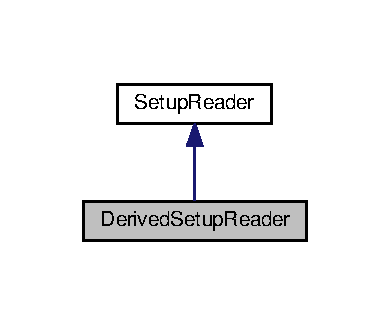
\includegraphics[width=187pt]{classDerivedSetupReader__inherit__graph}
\end{center}
\end{figure}


Collaboration diagram for Derived\+Setup\+Reader\+:
\nopagebreak
\begin{figure}[H]
\begin{center}
\leavevmode
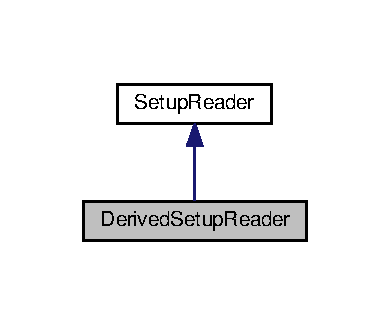
\includegraphics[width=187pt]{classDerivedSetupReader__coll__graph}
\end{center}
\end{figure}
\subsection*{Public Member Functions}
\begin{DoxyCompactItemize}
\item 
{\bfseries Derived\+Setup\+Reader} (std\+::string \&FN)\hypertarget{classDerivedSetupReader_a448acbcfdc7338dc35caa99af0b52dde}{}\label{classDerivedSetupReader_a448acbcfdc7338dc35caa99af0b52dde}

\end{DoxyCompactItemize}


The documentation for this class was generated from the following file\+:\begin{DoxyCompactItemize}
\item 
tests/Test\+Setup\+Reader.\+cpp\end{DoxyCompactItemize}

\hypertarget{classFixmanTorque}{}\section{Fixman\+Torque Class Reference}
\label{classFixmanTorque}\index{Fixman\+Torque@{Fixman\+Torque}}


Inheritance diagram for Fixman\+Torque\+:\nopagebreak
\begin{figure}[H]
\begin{center}
\leavevmode
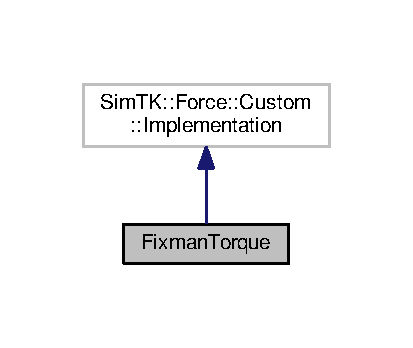
\includegraphics[width=198pt]{classFixmanTorque__inherit__graph}
\end{center}
\end{figure}


Collaboration diagram for Fixman\+Torque\+:\nopagebreak
\begin{figure}[H]
\begin{center}
\leavevmode
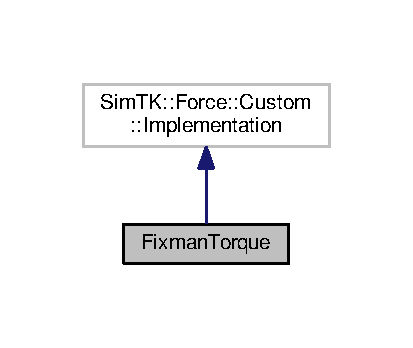
\includegraphics[width=198pt]{classFixmanTorque__coll__graph}
\end{center}
\end{figure}
\subsection*{Public Member Functions}
\begin{DoxyCompactItemize}
\item 
{\bfseries Fixman\+Torque} (Sim\+T\+K\+::\+Compound\+System $\ast$compound\+System, Sim\+T\+K\+::\+Simbody\+Matter\+Subsystem \&matter)\hypertarget{classFixmanTorque_a9d1922bbfbf57ff7e5ba329911819b63}{}\label{classFixmanTorque_a9d1922bbfbf57ff7e5ba329911819b63}

\item 
void {\bfseries calc\+Force} (const Sim\+T\+K\+::\+State \&state, Sim\+T\+K\+::\+Vector\+\_\+$<$ Sim\+T\+K\+::\+Spatial\+Vec $>$ \&body\+Forces, Sim\+T\+K\+::\+Vector\+\_\+$<$ Sim\+T\+K\+::\+Vec3 $>$ \&particle\+Forces, Sim\+T\+K\+::\+Vector \&mobility\+Forces) const override\hypertarget{classFixmanTorque_ace34df627e9380c393641d218348e4dc}{}\label{classFixmanTorque_ace34df627e9380c393641d218348e4dc}

\item 
Sim\+T\+K\+::\+Real {\bfseries calc\+Potential\+Energy} (const Sim\+T\+K\+::\+State \&state) const override\hypertarget{classFixmanTorque_a2b632689cbc3c2886f0a27f9fbeb27bb}{}\label{classFixmanTorque_a2b632689cbc3c2886f0a27f9fbeb27bb}

\item 
bool {\bfseries depends\+Only\+On\+Positions} () const \hypertarget{classFixmanTorque_ac751a14d42e46b96c26b935d64da27bd}{}\label{classFixmanTorque_ac751a14d42e46b96c26b935d64da27bd}

\item 
Sim\+T\+K\+::\+Real {\bfseries get\+Scale\+Factor} (void)\hypertarget{classFixmanTorque_a4330675bc902181bf25fcb1d75a1679e}{}\label{classFixmanTorque_a4330675bc902181bf25fcb1d75a1679e}

\item 
void {\bfseries set\+Scale\+Factor} (Sim\+T\+K\+::\+Real)\hypertarget{classFixmanTorque_a29c4bc51ed97d1f4223a5bcad3bd4fba}{}\label{classFixmanTorque_a29c4bc51ed97d1f4223a5bcad3bd4fba}

\item 
Sim\+T\+K\+::\+Real {\bfseries get\+Temperature} (void)\hypertarget{classFixmanTorque_a6d3bf8d4cb667226a9e320f59a4efc5f}{}\label{classFixmanTorque_a6d3bf8d4cb667226a9e320f59a4efc5f}

\item 
void {\bfseries set\+Temperature} (Sim\+T\+K\+::\+Real)\hypertarget{classFixmanTorque_a6e730f7d96c50020c793df3f4105997c}{}\label{classFixmanTorque_a6e730f7d96c50020c793df3f4105997c}

\end{DoxyCompactItemize}
\subsection*{Public Attributes}
\begin{DoxyCompactItemize}
\item 
Sim\+T\+K\+::\+Compound\+System $\ast$ {\bfseries compound\+System}\hypertarget{classFixmanTorque_ad14823bc66cdf8c9011b4244e25055a2}{}\label{classFixmanTorque_ad14823bc66cdf8c9011b4244e25055a2}

\item 
int $\ast$ {\bfseries flag}\hypertarget{classFixmanTorque_a79ebec738a8d217a768c485b619c8cba}{}\label{classFixmanTorque_a79ebec738a8d217a768c485b619c8cba}

\end{DoxyCompactItemize}


The documentation for this class was generated from the following files\+:\begin{DoxyCompactItemize}
\item 
include/gmolmodel/Fixman\+Torque.\+hpp\item 
src/Fixman\+Torque.\+cpp\end{DoxyCompactItemize}

\hypertarget{classGCHMCIntegrator}{}\section{G\+C\+H\+M\+C\+Integrator Class Reference}
\label{classGCHMCIntegrator}\index{G\+C\+H\+M\+C\+Integrator@{G\+C\+H\+M\+C\+Integrator}}


Collaboration diagram for G\+C\+H\+M\+C\+Integrator\+:\nopagebreak
\begin{figure}[H]
\begin{center}
\leavevmode
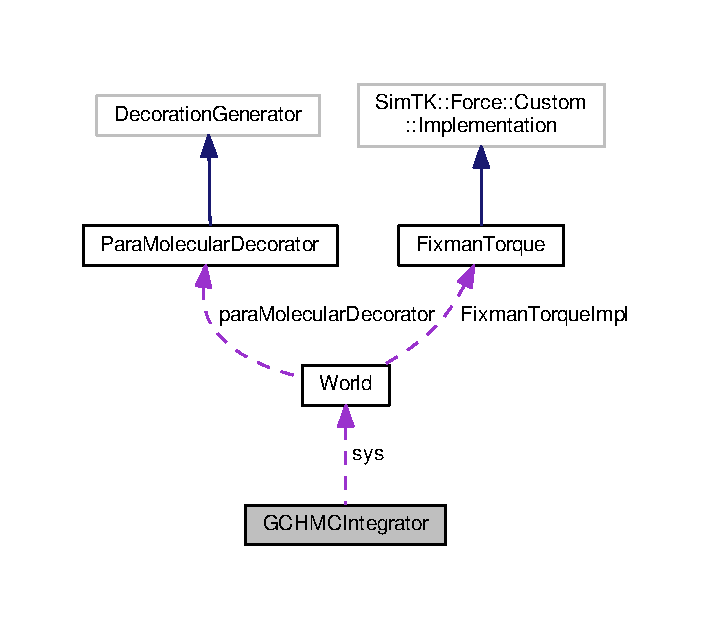
\includegraphics[width=343pt]{classGCHMCIntegrator__coll__graph}
\end{center}
\end{figure}
\subsection*{Public Member Functions}
\begin{DoxyCompactItemize}
\item 
{\bfseries G\+C\+H\+M\+C\+Integrator} (Py\+Object $\ast$, std\+::string, std\+::string)\hypertarget{classGCHMCIntegrator_ae32d76dd39c412ef0fda999102e2071a}{}\label{classGCHMCIntegrator_ae32d76dd39c412ef0fda999102e2071a}

\item 
boost\+::python\+::object {\bfseries Call} (int \+\_\+nosteps, int \+\_\+steps\+\_\+per\+\_\+trial, T\+A\+R\+G\+E\+T\+\_\+\+T\+Y\+PE \+\_\+temperature, T\+A\+R\+G\+E\+T\+\_\+\+T\+Y\+PE \+\_\+delta\+\_\+t, int \+\_\+pyseed, int \+\_\+mass\+Mat\+Num\+Opt, int \+\_\+metro\+Fixman\+Opt, double \+\_\+lj14sf)\hypertarget{classGCHMCIntegrator_abd20da7bc04de77b77cbe44d0af154e6}{}\label{classGCHMCIntegrator_abd20da7bc04de77b77cbe44d0af154e6}

\item 
void {\bfseries Clear} ()\hypertarget{classGCHMCIntegrator_a334218cacf7caf7d4d0026d7518f5a07}{}\label{classGCHMCIntegrator_a334218cacf7caf7d4d0026d7518f5a07}

\end{DoxyCompactItemize}
\subsection*{Public Attributes}
\begin{DoxyCompactItemize}
\item 
\hyperlink{classWorld}{World} $\ast$ {\bfseries sys}\hypertarget{classGCHMCIntegrator_a75299001f5c872307aa2e9eaf65d14a4}{}\label{classGCHMCIntegrator_a75299001f5c872307aa2e9eaf65d14a4}

\item 
T\+A\+R\+G\+E\+T\+\_\+\+T\+Y\+PE $\ast$ {\bfseries shm}\hypertarget{classGCHMCIntegrator_a1f11b96f92bf4e9bb80946fd3a69ae64}{}\label{classGCHMCIntegrator_a1f11b96f92bf4e9bb80946fd3a69ae64}

\item 
Py\+F\+F\+Evaluator\+Object $\ast$ {\bfseries py\+F\+F\+Evaluator\+Object}\hypertarget{classGCHMCIntegrator_a703999d22f28082ab7af71552848a171}{}\label{classGCHMCIntegrator_a703999d22f28082ab7af71552848a171}

\item 
energy\+\_\+data $\ast$ {\bfseries p\+\_\+energy\+\_\+po}\hypertarget{classGCHMCIntegrator_a756f6bdade73958cf355a302000eac5b}{}\label{classGCHMCIntegrator_a756f6bdade73958cf355a302000eac5b}

\item 
Py\+Array\+Object $\ast$ {\bfseries configuration}\hypertarget{classGCHMCIntegrator_ac25dd9aad3833746580d13ccd33e47d4}{}\label{classGCHMCIntegrator_ac25dd9aad3833746580d13ccd33e47d4}

\item 
Py\+Universe\+Spec\+Object $\ast$ {\bfseries universe\+\_\+spec}\hypertarget{classGCHMCIntegrator_acc088ddc60f6e5e24dcc2e6dce58829b}{}\label{classGCHMCIntegrator_acc088ddc60f6e5e24dcc2e6dce58829b}

\item 
Py\+Object $\ast$ {\bfseries universe}\hypertarget{classGCHMCIntegrator_aab32409e10bd4caae145b43e82d8f628}{}\label{classGCHMCIntegrator_aab32409e10bd4caae145b43e82d8f628}

\item 
Py\+Array\+Object $\ast$ {\bfseries gradarr}\hypertarget{classGCHMCIntegrator_aa4be68ee7df1067a9ef8a791a5e4ed3a}{}\label{classGCHMCIntegrator_aa4be68ee7df1067a9ef8a791a5e4ed3a}

\item 
int {\bfseries nosteps}\hypertarget{classGCHMCIntegrator_abb29657d59c4558c7e71e3dfeb869c3c}{}\label{classGCHMCIntegrator_abb29657d59c4558c7e71e3dfeb869c3c}

\item 
int {\bfseries ntrials}\hypertarget{classGCHMCIntegrator_a60ad501a60a7d798c9d8ec83a7c5087d}{}\label{classGCHMCIntegrator_a60ad501a60a7d798c9d8ec83a7c5087d}

\item 
int {\bfseries steps\+\_\+per\+\_\+trial}\hypertarget{classGCHMCIntegrator_a2e1cfdc645b8bed733ddc0694646779a}{}\label{classGCHMCIntegrator_a2e1cfdc645b8bed733ddc0694646779a}

\item 
double {\bfseries temperature}\hypertarget{classGCHMCIntegrator_af45d5b6c9e3b69be16412330c54186d2}{}\label{classGCHMCIntegrator_af45d5b6c9e3b69be16412330c54186d2}

\item 
double {\bfseries delta\+\_\+t}\hypertarget{classGCHMCIntegrator_a34a45de947a295da0f95ff5c3e414ade}{}\label{classGCHMCIntegrator_a34a45de947a295da0f95ff5c3e414ade}

\item 
int {\bfseries trouble}\hypertarget{classGCHMCIntegrator_a508ec016398bcd526e00bf8f209ba0db}{}\label{classGCHMCIntegrator_a508ec016398bcd526e00bf8f209ba0db}

\item 
int {\bfseries sweep}\hypertarget{classGCHMCIntegrator_a732a9e0fda0a6608eae84e5ec4e1d193}{}\label{classGCHMCIntegrator_a732a9e0fda0a6608eae84e5ec4e1d193}

\item 
int {\bfseries S\+H\+M\+SZ}\hypertarget{classGCHMCIntegrator_a437bd1a1a494f278a1bc41e3a754eac1}{}\label{classGCHMCIntegrator_a437bd1a1a494f278a1bc41e3a754eac1}

\end{DoxyCompactItemize}


The documentation for this class was generated from the following file\+:\begin{DoxyCompactItemize}
\item 
src/simmain.\+cpp\end{DoxyCompactItemize}

\hypertarget{classGirolamiSampler}{}\section{Girolami\+Sampler Class Reference}
\label{classGirolamiSampler}\index{Girolami\+Sampler@{Girolami\+Sampler}}


Inheritance diagram for Girolami\+Sampler\+:\nopagebreak
\begin{figure}[H]
\begin{center}
\leavevmode
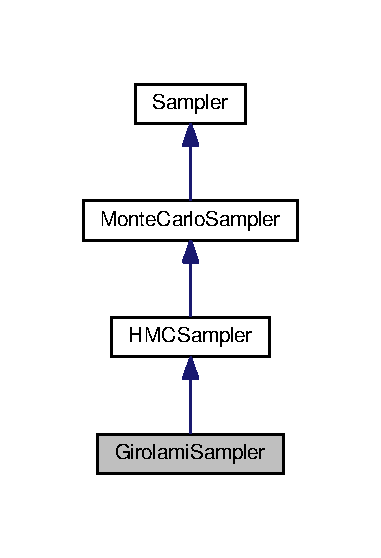
\includegraphics[width=183pt]{classGirolamiSampler__inherit__graph}
\end{center}
\end{figure}


Collaboration diagram for Girolami\+Sampler\+:\nopagebreak
\begin{figure}[H]
\begin{center}
\leavevmode
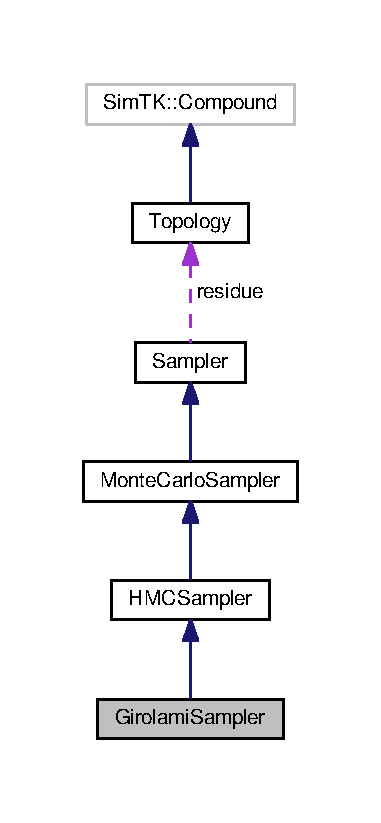
\includegraphics[width=183pt]{classGirolamiSampler__coll__graph}
\end{center}
\end{figure}
\subsection*{Public Member Functions}
\begin{DoxyCompactItemize}
\item 
{\bfseries Girolami\+Sampler} (Sim\+T\+K\+::\+Compound\+System $\ast$arg\+Compound\+System, Sim\+T\+K\+::\+Simbody\+Matter\+Subsystem $\ast$arg\+Matter, std\+::vector$<$ \hyperlink{classTopology}{Topology} $\ast$ $>$ \&topologies, Sim\+T\+K\+::\+Du\+M\+M\+Force\+Field\+Subsystem $\ast$arg\+Dumm, Sim\+T\+K\+::\+General\+Force\+Subsystem $\ast$forces, Sim\+T\+K\+::\+Time\+Stepper $\ast$arg\+Time\+Stepper)\hypertarget{classGirolamiSampler_a45a3f2334ac7cf244bab902304be9e3b}{}\label{classGirolamiSampler_a45a3f2334ac7cf244bab902304be9e3b}

\item 
virtual \hyperlink{classGirolamiSampler_afdf9a9d83f383611cdfc4226e76f70f7}{$\sim$\+Girolami\+Sampler} ()
\item 
virtual void \hyperlink{classGirolamiSampler_a1e48f38fa966f7063f190bba32193b42}{initialize} (Sim\+T\+K\+::\+State \&advanced, Sim\+T\+K\+::\+Real \hyperlink{classHMCSampler_a8cd8b25b42e94acb34aa0dea64c67b5b}{timestep}, int nosteps, Sim\+T\+K\+::\+Real arg\+Temperature, bool arg\+Use\+Fixman=true)
\item 
virtual void \hyperlink{classGirolamiSampler_a60a0994ea481381dd2596a711d839f5d}{reinitialize} (Sim\+T\+K\+::\+State \&advanced, Sim\+T\+K\+::\+Real \hyperlink{classHMCSampler_a8cd8b25b42e94acb34aa0dea64c67b5b}{timestep}, int nosteps, Sim\+T\+K\+::\+Real arg\+Temperature)
\item 
void \hyperlink{classGirolamiSampler_ad5b07ddfcab269774723a8156670ee28}{propose} (Sim\+T\+K\+::\+State \&some\+State, Sim\+T\+K\+::\+Real \hyperlink{classHMCSampler_a8cd8b25b42e94acb34aa0dea64c67b5b}{timestep}, int nosteps)
\item 
void \hyperlink{classGirolamiSampler_aef18692e13adaa564a9106e94a801893}{update} (Sim\+T\+K\+::\+State \&some\+State, Sim\+T\+K\+::\+Real \hyperlink{classHMCSampler_a8cd8b25b42e94acb34aa0dea64c67b5b}{timestep}, int nosteps)
\end{DoxyCompactItemize}
\subsection*{Protected Attributes}
\begin{DoxyCompactItemize}
\item 
bool {\bfseries use\+Fixman\+Torque} = true\hypertarget{classGirolamiSampler_a6f81b5defa538906e80690464b7102b6}{}\label{classGirolamiSampler_a6f81b5defa538906e80690464b7102b6}

\end{DoxyCompactItemize}
\subsection*{Additional Inherited Members}


\subsection{Constructor \& Destructor Documentation}
\index{Girolami\+Sampler@{Girolami\+Sampler}!````~Girolami\+Sampler@{$\sim$\+Girolami\+Sampler}}
\index{````~Girolami\+Sampler@{$\sim$\+Girolami\+Sampler}!Girolami\+Sampler@{Girolami\+Sampler}}
\subsubsection[{\texorpdfstring{$\sim$\+Girolami\+Sampler()}{~GirolamiSampler()}}]{\setlength{\rightskip}{0pt plus 5cm}Girolami\+Sampler\+::$\sim$\+Girolami\+Sampler (
\begin{DoxyParamCaption}
{}
\end{DoxyParamCaption}
)\hspace{0.3cm}{\ttfamily [virtual]}}\hypertarget{classGirolamiSampler_afdf9a9d83f383611cdfc4226e76f70f7}{}\label{classGirolamiSampler_afdf9a9d83f383611cdfc4226e76f70f7}
Destructor 

\subsection{Member Function Documentation}
\index{Girolami\+Sampler@{Girolami\+Sampler}!initialize@{initialize}}
\index{initialize@{initialize}!Girolami\+Sampler@{Girolami\+Sampler}}
\subsubsection[{\texorpdfstring{initialize(\+Sim\+T\+K\+::\+State \&advanced, Sim\+T\+K\+::\+Real timestep, int nosteps, Sim\+T\+K\+::\+Real arg\+Temperature, bool arg\+Use\+Fixman=true)}{initialize(SimTK::State &advanced, SimTK::Real timestep, int nosteps, SimTK::Real argTemperature, bool argUseFixman=true)}}]{\setlength{\rightskip}{0pt plus 5cm}void Girolami\+Sampler\+::initialize (
\begin{DoxyParamCaption}
\item[{Sim\+T\+K\+::\+State \&}]{some\+State, }
\item[{Sim\+T\+K\+::\+Real}]{timestep, }
\item[{int}]{nosteps, }
\item[{Sim\+T\+K\+::\+Real}]{arg\+Temperature, }
\item[{bool}]{arg\+Use\+Fixman = {\ttfamily true}}
\end{DoxyParamCaption}
)\hspace{0.3cm}{\ttfamily [virtual]}}\hypertarget{classGirolamiSampler_a1e48f38fa966f7063f190bba32193b42}{}\label{classGirolamiSampler_a1e48f38fa966f7063f190bba32193b42}
Seed the random number generator. Set simulation temperature, velocities to desired temperature, variables that store the configuration and variables that store the energies, both needed for the acception-\/rejection step. Also realize velocities and initialize the timestepper. \index{Girolami\+Sampler@{Girolami\+Sampler}!propose@{propose}}
\index{propose@{propose}!Girolami\+Sampler@{Girolami\+Sampler}}
\subsubsection[{\texorpdfstring{propose(\+Sim\+T\+K\+::\+State \&some\+State, Sim\+T\+K\+::\+Real timestep, int nosteps)}{propose(SimTK::State &someState, SimTK::Real timestep, int nosteps)}}]{\setlength{\rightskip}{0pt plus 5cm}void Girolami\+Sampler\+::propose (
\begin{DoxyParamCaption}
\item[{Sim\+T\+K\+::\+State \&}]{some\+State, }
\item[{Sim\+T\+K\+::\+Real}]{timestep, }
\item[{int}]{nosteps}
\end{DoxyParamCaption}
)}\hypertarget{classGirolamiSampler_ad5b07ddfcab269774723a8156670ee28}{}\label{classGirolamiSampler_ad5b07ddfcab269774723a8156670ee28}
It implements the proposal move in the Hamiltonian Monte Carlo algorithm. It essentially propagates the trajectory after it stores the configuration and energies. T\+O\+DO\+: break in two functions\+: initialize\+Velocities and propagate/integrate \index{Girolami\+Sampler@{Girolami\+Sampler}!reinitialize@{reinitialize}}
\index{reinitialize@{reinitialize}!Girolami\+Sampler@{Girolami\+Sampler}}
\subsubsection[{\texorpdfstring{reinitialize(\+Sim\+T\+K\+::\+State \&advanced, Sim\+T\+K\+::\+Real timestep, int nosteps, Sim\+T\+K\+::\+Real arg\+Temperature)}{reinitialize(SimTK::State &advanced, SimTK::Real timestep, int nosteps, SimTK::Real argTemperature)}}]{\setlength{\rightskip}{0pt plus 5cm}void Girolami\+Sampler\+::reinitialize (
\begin{DoxyParamCaption}
\item[{Sim\+T\+K\+::\+State \&}]{some\+State, }
\item[{Sim\+T\+K\+::\+Real}]{timestep, }
\item[{int}]{nosteps, }
\item[{Sim\+T\+K\+::\+Real}]{arg\+Temperature}
\end{DoxyParamCaption}
)\hspace{0.3cm}{\ttfamily [virtual]}}\hypertarget{classGirolamiSampler_a60a0994ea481381dd2596a711d839f5d}{}\label{classGirolamiSampler_a60a0994ea481381dd2596a711d839f5d}
Same as initialize \index{Girolami\+Sampler@{Girolami\+Sampler}!update@{update}}
\index{update@{update}!Girolami\+Sampler@{Girolami\+Sampler}}
\subsubsection[{\texorpdfstring{update(\+Sim\+T\+K\+::\+State \&some\+State, Sim\+T\+K\+::\+Real timestep, int nosteps)}{update(SimTK::State &someState, SimTK::Real timestep, int nosteps)}}]{\setlength{\rightskip}{0pt plus 5cm}void Girolami\+Sampler\+::update (
\begin{DoxyParamCaption}
\item[{Sim\+T\+K\+::\+State \&}]{some\+State, }
\item[{Sim\+T\+K\+::\+Real}]{timestep, }
\item[{int}]{nosteps}
\end{DoxyParamCaption}
)}\hypertarget{classGirolamiSampler_aef18692e13adaa564a9106e94a801893}{}\label{classGirolamiSampler_aef18692e13adaa564a9106e94a801893}
Main function that contains all the 3 steps of H\+MC. Implements the acception-\/rejection step and sets the state of the compound to the appropriate conformation wether it accepted or not. 

The documentation for this class was generated from the following files\+:\begin{DoxyCompactItemize}
\item 
include/gmolmodel/Girolami\+Sampler.\+hpp\item 
src/\hyperlink{GirolamiSampler_8cpp}{Girolami\+Sampler.\+cpp}\end{DoxyCompactItemize}

\hypertarget{classHMCSampler}{}\section{H\+M\+C\+Sampler Class Reference}
\label{classHMCSampler}\index{H\+M\+C\+Sampler@{H\+M\+C\+Sampler}}


{\ttfamily \#include $<$H\+M\+C\+Sampler.\+hpp$>$}



Inheritance diagram for H\+M\+C\+Sampler\+:\nopagebreak
\begin{figure}[H]
\begin{center}
\leavevmode
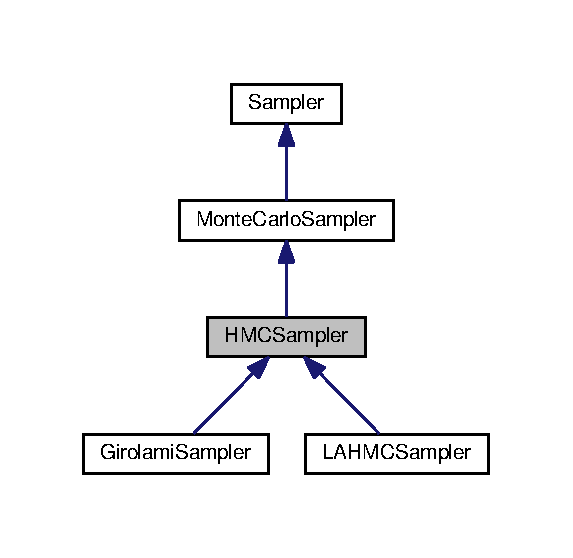
\includegraphics[width=275pt]{classHMCSampler__inherit__graph}
\end{center}
\end{figure}


Collaboration diagram for H\+M\+C\+Sampler\+:\nopagebreak
\begin{figure}[H]
\begin{center}
\leavevmode
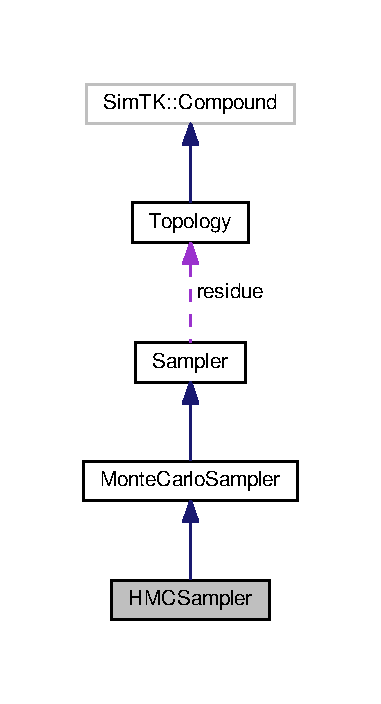
\includegraphics[width=183pt]{classHMCSampler__coll__graph}
\end{center}
\end{figure}
\subsection*{Public Member Functions}
\begin{DoxyCompactItemize}
\item 
\hyperlink{classHMCSampler_abfc3165e0a559567e33bf19b8aea1a47}{H\+M\+C\+Sampler} (Sim\+T\+K\+::\+Compound\+System $\ast$arg\+Compound\+System, Sim\+T\+K\+::\+Simbody\+Matter\+Subsystem $\ast$arg\+Matter, std\+::vector$<$ \hyperlink{classTopology}{Topology} $\ast$ $>$ \&arg\+Topologies, Sim\+T\+K\+::\+Du\+M\+M\+Force\+Field\+Subsystem $\ast$arg\+Dumm, Sim\+T\+K\+::\+General\+Force\+Subsystem $\ast$forces, Sim\+T\+K\+::\+Time\+Stepper $\ast$arg\+Time\+Stepper)
\item 
virtual \hyperlink{classHMCSampler_a1781a161d1a712ed28c973b4b56c3c7f}{$\sim$\+H\+M\+C\+Sampler} ()
\item 
void \hyperlink{classHMCSampler_a1335bea08f96d449cb9bdb985b3e6b9d}{calc\+Sqrt\+M\+InvL} (Sim\+T\+K\+::\+State \&some\+State, Sim\+T\+K\+::\+Matrix \&Sqrt\+M\+Inv)
\item 
void \hyperlink{classHMCSampler_ab4f9446e1b9ecb3f47b62637e8bc6fb9}{calc\+Sqrt\+M\+InvU} (Sim\+T\+K\+::\+State \&some\+State, Sim\+T\+K\+::\+Matrix \&Sqrt\+M\+Inv)
\item 
void \hyperlink{classHMCSampler_ad47e283497806a105dac3c2b15127fbf}{calc\+Num\+Sqrt\+M\+Upper} (Sim\+T\+K\+::\+State \&some\+State, Sim\+T\+K\+::\+Matrix \&Sqrt\+M\+Upper)
\item 
virtual void \hyperlink{classHMCSampler_ad878471d3e5222758b2544f76affd79a}{initialize} (Sim\+T\+K\+::\+State \&advanced)
\item 
virtual void \hyperlink{classHMCSampler_a43a302d87e149bfa893a5952ec20941f}{reinitialize} (Sim\+T\+K\+::\+State \&advanced)
\item 
const Sim\+T\+K\+::\+Time\+Stepper $\ast$ \hyperlink{classHMCSampler_a90d64460a0b1b4e83e3c27db0b7681f0}{get\+Time\+Stepper} (void)
\item 
Sim\+T\+K\+::\+Time\+Stepper $\ast$ {\bfseries upd\+Time\+Stepper} (void)\hypertarget{classHMCSampler_a16ecb11f6a9943d42a63448acb4358c4}{}\label{classHMCSampler_a16ecb11f6a9943d42a63448acb4358c4}

\item 
void {\bfseries set\+Time\+Stepper} (Sim\+T\+K\+::\+Time\+Stepper $\ast$some\+Time\+Stepper)\hypertarget{classHMCSampler_a7d8cfa2e3ff72ede9e3136d3a709ad43}{}\label{classHMCSampler_a7d8cfa2e3ff72ede9e3136d3a709ad43}

\item 
virtual float \hyperlink{classHMCSampler_ab8fb503782cc7fe6951b5189802d174d}{get\+Timestep} (void)
\item 
virtual void {\bfseries set\+Timestep} (float)\hypertarget{classHMCSampler_a47f010ac63622ca8a1f758db5c21e37b}{}\label{classHMCSampler_a47f010ac63622ca8a1f758db5c21e37b}

\item 
Sim\+T\+K\+::\+Real \hyperlink{classHMCSampler_a97914f58682cd08bacffc115e91499e1}{get\+Boost\+Temperature} (void)
\item 
void {\bfseries set\+Boost\+Temperature} (Sim\+T\+K\+::\+Real)\hypertarget{classHMCSampler_a121c0aa27c531b046215daeb8b4e94b4}{}\label{classHMCSampler_a121c0aa27c531b046215daeb8b4e94b4}

\item 
void {\bfseries set\+Boost\+M\+D\+Steps} (int)\hypertarget{classHMCSampler_aa2c6aec792fb63dc1ecd7d372a5867a9}{}\label{classHMCSampler_aa2c6aec792fb63dc1ecd7d372a5867a9}

\item 
virtual void \hyperlink{classHMCSampler_a8c9a03dba406c0d4bef622c42d399b19}{store\+Old\+Configuration\+And\+Potential\+Energies} (Sim\+T\+K\+::\+State \&some\+State)
\item 
virtual void \hyperlink{classHMCSampler_ae38d8206113980732d4adced081c50fd}{initialize\+Velocities} (Sim\+T\+K\+::\+State \&some\+State)
\item 
virtual void \hyperlink{classHMCSampler_a492f12a031effba381c409052ab734e7}{calc\+Proposed\+Kinetic\+And\+Total\+Energy} (Sim\+T\+K\+::\+State \&some\+State)
\item 
virtual void \hyperlink{classHMCSampler_ab3b4de64be2a10193e274f05788b5ca5}{integrate\+Trajectory} (Sim\+T\+K\+::\+State \&some\+State)
\item 
virtual void \hyperlink{classHMCSampler_a4e74ce67f749317e106a528e2791df9d}{integrate\+Trajectory\+One\+Step\+At\+A\+Time} (Sim\+T\+K\+::\+State \&some\+State)
\item 
virtual void \hyperlink{classHMCSampler_aa3b0a772e2ba3ea1550ec834e887fc67}{adapt\+Timestep} (Sim\+T\+K\+::\+State \&some\+State)
\item 
void \hyperlink{classHMCSampler_a90ffe962e5317623389f4db7a85e0592}{adapt\+World\+Blocks} (Sim\+T\+K\+::\+State \&some\+State)
\item 
virtual void \hyperlink{classHMCSampler_a4716c29b164a3f9f239266e970498201}{calc\+New\+Configuration\+And\+Energies} (Sim\+T\+K\+::\+State \&some\+State)
\item 
virtual void \hyperlink{classHMCSampler_a26452f17a85fadebcf44bddb44954cc6}{set\+Set\+Configuration\+And\+Energies\+To\+Old} (Sim\+T\+K\+::\+State \&some\+State)
\item 
virtual void \hyperlink{classHMCSampler_a4deb485f9bfc31d64f6ada06536f9230}{set\+Set\+Configuration\+And\+Energies\+To\+New} (Sim\+T\+K\+::\+State \&some\+State)
\item 
virtual Sim\+T\+K\+::\+Real \hyperlink{classHMCSampler_a7fee5ad6d531c32235db96c4b95f1eca}{M\+H\+Accept\+Probability} (Sim\+T\+K\+::\+State \&some\+State, Sim\+T\+K\+::\+Real arg\+Etot\+\_\+proposed, Sim\+T\+K\+::\+Real arg\+Etot\+\_\+n)
\item 
virtual bool \hyperlink{classHMCSampler_af5e87c855b8888196a9f2ad87bb9f824}{acc\+Rej\+Step} (Sim\+T\+K\+::\+State \&some\+State)
\item 
void \hyperlink{classHMCSampler_aa36ab4482bbb6295658e8fe6a49c9e4f}{propose} (Sim\+T\+K\+::\+State \&some\+State)
\item 
void \hyperlink{classHMCSampler_a864175524b6023f505357b10b1a5855b}{update} (Sim\+T\+K\+::\+State \&some\+State)
\item 
virtual bool {\bfseries sample\+\_\+iteration} (Sim\+T\+K\+::\+State \&some\+State)\hypertarget{classHMCSampler_ae27a31bb0f1e6b71c830db555ca97d2f}{}\label{classHMCSampler_ae27a31bb0f1e6b71c830db555ca97d2f}

\item 
int \hyperlink{classHMCSampler_a4c2bd08867d1a07c54587d52fd8d5fed}{push\+Coordinates\+InR} (Sim\+T\+K\+::\+State \&some\+State)
\item 
int \hyperlink{classHMCSampler_a8e67589e5d96c6fe11a20f7bc073af84}{push\+Velocities\+In\+Rdot} (Sim\+T\+K\+::\+State \&some\+State)
\item 
int \hyperlink{classHMCSampler_aa0e27f4d44328dcae4a2a38cf1b3f626}{push\+Coordinates\+InQ} (Sim\+T\+K\+::\+State \&some\+State)
\item 
int \hyperlink{classHMCSampler_a642722a3022575f342c9913ffbb82ce2}{push\+Velocities\+In\+Qdot} (Sim\+T\+K\+::\+State \&some\+State)
\item 
int \hyperlink{classHMCSampler_abcdb1f372e12dabec50d4f674c708461}{push\+Velocities\+InU} (Sim\+T\+K\+::\+State \&some\+State)
\item 
void \hyperlink{classHMCSampler_a4abf0550ceb1ecef10c5823581ebf515}{perturbQ} (Sim\+T\+K\+::\+State \&some\+State)
\item 
Sim\+T\+K\+::\+Real \hyperlink{classHMCSampler_aea854d56098d31f7b2e2d15d231b8949}{get\+Proposed\+KE} (void)
\item 
Sim\+T\+K\+::\+Real \hyperlink{classHMCSampler_a1e3d6ded4ceb757ab402e6ace268fc2b}{get\+Last\+Accepted\+KE} (void)
\item 
void \hyperlink{classHMCSampler_a5972926e31fe4f9ee7ae1498f049f9f1}{set\+Proposed\+KE} (Sim\+T\+K\+::\+Real)
\item 
void \hyperlink{classHMCSampler_a44b541a914af643eaca56e43d5d58a13}{set\+Last\+Accepted\+KE} (Sim\+T\+K\+::\+Real)
\item 
int {\bfseries get\+M\+D\+Steps\+Per\+Sample} () const \hypertarget{classHMCSampler_a8e67512f7f8f3bcfe4a736f8b871703c}{}\label{classHMCSampler_a8e67512f7f8f3bcfe4a736f8b871703c}

\item 
void {\bfseries set\+M\+D\+Steps\+Per\+Sample} (int md\+Steps\+Per\+Sample)\hypertarget{classHMCSampler_a4a65fde374fba7362ef1f3d37f3a79da}{}\label{classHMCSampler_a4a65fde374fba7362ef1f3d37f3a79da}

\item 
void \hyperlink{classHMCSampler_ab0354537f83779a468255e4c5fc2c9b6}{Print\+Detailed\+Energy\+Info} (Sim\+T\+K\+::\+State \&some\+State)
\item 
Sim\+T\+K\+::\+Real \hyperlink{classHMCSampler_a36bce5b70cae7391ff300b0ca834b84f}{calculate\+M\+SD} (void)
\item 
Sim\+T\+K\+::\+Real \hyperlink{classHMCSampler_a9d64c28ce62364363fe7c1ff3baceefa}{calculate\+R\+Rdot} (void)
\item 
void {\bfseries geom\+Dihedral} (void)\hypertarget{classHMCSampler_a9e262ad1a8b9a9d70d6f52d8a638567b}{}\label{classHMCSampler_a9e262ad1a8b9a9d70d6f52d8a638567b}

\end{DoxyCompactItemize}
\subsection*{Protected Attributes}
\begin{DoxyCompactItemize}
\item 
float \hyperlink{classHMCSampler_a8cd8b25b42e94acb34aa0dea64c67b5b}{timestep}
\item 
float {\bfseries prev\+Timestep}\hypertarget{classHMCSampler_a8ae12739d6e0fce6e22d26e0e90d67a8}{}\label{classHMCSampler_a8ae12739d6e0fce6e22d26e0e90d67a8}

\item 
float {\bfseries prev\+Prev\+Timestep}\hypertarget{classHMCSampler_a061efabb2c1486e64b6b2cbc9cab0245}{}\label{classHMCSampler_a061efabb2c1486e64b6b2cbc9cab0245}

\item 
bool {\bfseries should\+Adapt\+Timestep}\hypertarget{classHMCSampler_ae573472509f1c59add03d72f753c4f06}{}\label{classHMCSampler_ae573472509f1c59add03d72f753c4f06}

\item 
Sim\+T\+K\+::\+Real {\bfseries ke\+\_\+last\+Accepted}\hypertarget{classHMCSampler_a73f309b15007ce520f6117080975da6d}{}\label{classHMCSampler_a73f309b15007ce520f6117080975da6d}

\item 
Sim\+T\+K\+::\+Real {\bfseries ke\+\_\+proposed}\hypertarget{classHMCSampler_a969e707966ce88fd12b21a86bc60f7bf}{}\label{classHMCSampler_a969e707966ce88fd12b21a86bc60f7bf}

\item 
Sim\+T\+K\+::\+Real {\bfseries ke\+\_\+n}\hypertarget{classHMCSampler_aa13c23e6ba3ebe6222228285fd94c4a4}{}\label{classHMCSampler_aa13c23e6ba3ebe6222228285fd94c4a4}

\item 
Sim\+T\+K\+::\+Real {\bfseries etot\+\_\+set}\hypertarget{classHMCSampler_a3dfcb5672d86f951f647068099165923}{}\label{classHMCSampler_a3dfcb5672d86f951f647068099165923}

\item 
Sim\+T\+K\+::\+Real {\bfseries etot\+\_\+proposed}\hypertarget{classHMCSampler_af3693cc4c5cf76ce9dce559b702c699c}{}\label{classHMCSampler_af3693cc4c5cf76ce9dce559b702c699c}

\item 
Sim\+T\+K\+::\+Real {\bfseries etot\+\_\+n}\hypertarget{classHMCSampler_ab39e667c819a1e0354d765ba5418a717}{}\label{classHMCSampler_ab39e667c819a1e0354d765ba5418a717}

\item 
Sim\+T\+K\+::\+Real {\bfseries boostT}\hypertarget{classHMCSampler_a709f4760098c1ce280793e0eb0ef0dca}{}\label{classHMCSampler_a709f4760098c1ce280793e0eb0ef0dca}

\item 
Sim\+T\+K\+::\+Real {\bfseries boost\+Factor}\hypertarget{classHMCSampler_af0ccf6cd8e96cbaf55ccdebbb55e4419}{}\label{classHMCSampler_af0ccf6cd8e96cbaf55ccdebbb55e4419}

\item 
Sim\+T\+K\+::\+Real {\bfseries unboost\+Factor}\hypertarget{classHMCSampler_a799ed5a2c3e212576f0f11ba89a86343}{}\label{classHMCSampler_a799ed5a2c3e212576f0f11ba89a86343}

\item 
int {\bfseries boost\+M\+D\+Steps}\hypertarget{classHMCSampler_a6b9ff11f9edc77345ba2c7bdfd5887a8}{}\label{classHMCSampler_a6b9ff11f9edc77345ba2c7bdfd5887a8}

\item 
int {\bfseries M\+D\+Steps\+Per\+Sample}\hypertarget{classHMCSampler_addee9ed20989678559ed764c114fe04c}{}\label{classHMCSampler_addee9ed20989678559ed764c114fe04c}

\item 
std\+::vector$<$ Sim\+T\+K\+::\+Real $>$ {\bfseries R}\hypertarget{classHMCSampler_a960f036573f204c55f105af554777e8f}{}\label{classHMCSampler_a960f036573f204c55f105af554777e8f}

\item 
std\+::vector$<$ Sim\+T\+K\+::\+Real $>$ {\bfseries Rdot}\hypertarget{classHMCSampler_a5f4d839058ef10a0e6c4ecf998f5d05f}{}\label{classHMCSampler_a5f4d839058ef10a0e6c4ecf998f5d05f}

\item 
std\+::vector$<$ Sim\+T\+K\+::\+Real $>$ {\bfseries dR}\hypertarget{classHMCSampler_a95e917dbcb8595d292add5e618ac5559}{}\label{classHMCSampler_a95e917dbcb8595d292add5e618ac5559}

\item 
std\+::vector$<$ Sim\+T\+K\+::\+Real $>$ {\bfseries d\+Rdot}\hypertarget{classHMCSampler_a0f5b2c1ecfc84755be4da47d89ebbb68}{}\label{classHMCSampler_a0f5b2c1ecfc84755be4da47d89ebbb68}

\end{DoxyCompactItemize}
\subsection*{Friends}
\begin{DoxyCompactItemize}
\item 
class {\bfseries Context}\hypertarget{classHMCSampler_ac26c806e60ca4a0547680edb68f6e39b}{}\label{classHMCSampler_ac26c806e60ca4a0547680edb68f6e39b}

\end{DoxyCompactItemize}
\subsection*{Additional Inherited Members}


\subsection{Detailed Description}
A Generalized Coordiantes Hamiltonian Monte Carlo sampler as described in J Chem Theory Comput. 2017 Oct 10;13(10)\+:4649-\/4659. In short it consists of the following steps\+:
\begin{DoxyEnumerate}
\item Initialize velocities from a random normal distribution with a covariance of kT sqrt(\+M) where M is the mass matrix tensor.
\item Propagate the trial trajectory using a symplectic integrator provided by Simbody
\item An acception-\/rejection step which includes the Fixman potential if needed. Step 1 and 2 are implemented in the fuction propose. Step 3 is implemented in the function update. 
\end{DoxyEnumerate}

\subsection{Constructor \& Destructor Documentation}
\index{H\+M\+C\+Sampler@{H\+M\+C\+Sampler}!H\+M\+C\+Sampler@{H\+M\+C\+Sampler}}
\index{H\+M\+C\+Sampler@{H\+M\+C\+Sampler}!H\+M\+C\+Sampler@{H\+M\+C\+Sampler}}
\subsubsection[{\texorpdfstring{H\+M\+C\+Sampler(\+Sim\+T\+K\+::\+Compound\+System $\ast$arg\+Compound\+System, Sim\+T\+K\+::\+Simbody\+Matter\+Subsystem $\ast$arg\+Matter, std\+::vector$<$ Topology $\ast$ $>$ \&arg\+Topologies, Sim\+T\+K\+::\+Du\+M\+M\+Force\+Field\+Subsystem $\ast$arg\+Dumm, Sim\+T\+K\+::\+General\+Force\+Subsystem $\ast$forces, Sim\+T\+K\+::\+Time\+Stepper $\ast$arg\+Time\+Stepper)}{HMCSampler(SimTK::CompoundSystem *argCompoundSystem, SimTK::SimbodyMatterSubsystem *argMatter, std::vector< Topology * > &argTopologies, SimTK::DuMMForceFieldSubsystem *argDumm, SimTK::GeneralForceSubsystem *forces, SimTK::TimeStepper *argTimeStepper)}}]{\setlength{\rightskip}{0pt plus 5cm}H\+M\+C\+Sampler\+::\+H\+M\+C\+Sampler (
\begin{DoxyParamCaption}
\item[{Sim\+T\+K\+::\+Compound\+System $\ast$}]{arg\+Compound\+System, }
\item[{Sim\+T\+K\+::\+Simbody\+Matter\+Subsystem $\ast$}]{arg\+Matter, }
\item[{std\+::vector$<$ {\bf Topology} $\ast$ $>$ \&}]{arg\+Topologies, }
\item[{Sim\+T\+K\+::\+Du\+M\+M\+Force\+Field\+Subsystem $\ast$}]{arg\+Dumm, }
\item[{Sim\+T\+K\+::\+General\+Force\+Subsystem $\ast$}]{forces, }
\item[{Sim\+T\+K\+::\+Time\+Stepper $\ast$}]{arg\+Time\+Stepper}
\end{DoxyParamCaption}
)}\hypertarget{classHMCSampler_abfc3165e0a559567e33bf19b8aea1a47}{}\label{classHMCSampler_abfc3165e0a559567e33bf19b8aea1a47}
Constructor \index{H\+M\+C\+Sampler@{H\+M\+C\+Sampler}!````~H\+M\+C\+Sampler@{$\sim$\+H\+M\+C\+Sampler}}
\index{````~H\+M\+C\+Sampler@{$\sim$\+H\+M\+C\+Sampler}!H\+M\+C\+Sampler@{H\+M\+C\+Sampler}}
\subsubsection[{\texorpdfstring{$\sim$\+H\+M\+C\+Sampler()}{~HMCSampler()}}]{\setlength{\rightskip}{0pt plus 5cm}H\+M\+C\+Sampler\+::$\sim$\+H\+M\+C\+Sampler (
\begin{DoxyParamCaption}
{}
\end{DoxyParamCaption}
)\hspace{0.3cm}{\ttfamily [virtual]}}\hypertarget{classHMCSampler_a1781a161d1a712ed28c973b4b56c3c7f}{}\label{classHMCSampler_a1781a161d1a712ed28c973b4b56c3c7f}
Destructor 

\subsection{Member Function Documentation}
\index{H\+M\+C\+Sampler@{H\+M\+C\+Sampler}!acc\+Rej\+Step@{acc\+Rej\+Step}}
\index{acc\+Rej\+Step@{acc\+Rej\+Step}!H\+M\+C\+Sampler@{H\+M\+C\+Sampler}}
\subsubsection[{\texorpdfstring{acc\+Rej\+Step(\+Sim\+T\+K\+::\+State \&some\+State)}{accRejStep(SimTK::State &someState)}}]{\setlength{\rightskip}{0pt plus 5cm}bool H\+M\+C\+Sampler\+::acc\+Rej\+Step (
\begin{DoxyParamCaption}
\item[{Sim\+T\+K\+::\+State \&}]{some\+State}
\end{DoxyParamCaption}
)\hspace{0.3cm}{\ttfamily [virtual]}}\hypertarget{classHMCSampler_af5e87c855b8888196a9f2ad87bb9f824}{}\label{classHMCSampler_af5e87c855b8888196a9f2ad87bb9f824}
Accetion rejection step

Acception rejection step 

Reimplemented in \hyperlink{classLAHMCSampler_a0baac57ec1fe8d795a6fea65acdf86ed}{L\+A\+H\+M\+C\+Sampler}.

\index{H\+M\+C\+Sampler@{H\+M\+C\+Sampler}!adapt\+Timestep@{adapt\+Timestep}}
\index{adapt\+Timestep@{adapt\+Timestep}!H\+M\+C\+Sampler@{H\+M\+C\+Sampler}}
\subsubsection[{\texorpdfstring{adapt\+Timestep(\+Sim\+T\+K\+::\+State \&some\+State)}{adaptTimestep(SimTK::State &someState)}}]{\setlength{\rightskip}{0pt plus 5cm}void H\+M\+C\+Sampler\+::adapt\+Timestep (
\begin{DoxyParamCaption}
\item[{Sim\+T\+K\+::\+State \&}]{some\+State}
\end{DoxyParamCaption}
)\hspace{0.3cm}{\ttfamily [virtual]}}\hypertarget{classHMCSampler_aa3b0a772e2ba3ea1550ec834e887fc67}{}\label{classHMCSampler_aa3b0a772e2ba3ea1550ec834e887fc67}
Use stochastic optimization to adapt timestep \index{H\+M\+C\+Sampler@{H\+M\+C\+Sampler}!adapt\+World\+Blocks@{adapt\+World\+Blocks}}
\index{adapt\+World\+Blocks@{adapt\+World\+Blocks}!H\+M\+C\+Sampler@{H\+M\+C\+Sampler}}
\subsubsection[{\texorpdfstring{adapt\+World\+Blocks(\+Sim\+T\+K\+::\+State \&some\+State)}{adaptWorldBlocks(SimTK::State &someState)}}]{\setlength{\rightskip}{0pt plus 5cm}void H\+M\+C\+Sampler\+::adapt\+World\+Blocks (
\begin{DoxyParamCaption}
\item[{Sim\+T\+K\+::\+State \&}]{some\+State}
\end{DoxyParamCaption}
)}\hypertarget{classHMCSampler_a90ffe962e5317623389f4db7a85e0592}{}\label{classHMCSampler_a90ffe962e5317623389f4db7a85e0592}
Adapt Gibbs blocks definitions \index{H\+M\+C\+Sampler@{H\+M\+C\+Sampler}!calc\+New\+Configuration\+And\+Energies@{calc\+New\+Configuration\+And\+Energies}}
\index{calc\+New\+Configuration\+And\+Energies@{calc\+New\+Configuration\+And\+Energies}!H\+M\+C\+Sampler@{H\+M\+C\+Sampler}}
\subsubsection[{\texorpdfstring{calc\+New\+Configuration\+And\+Energies(\+Sim\+T\+K\+::\+State \&some\+State)}{calcNewConfigurationAndEnergies(SimTK::State &someState)}}]{\setlength{\rightskip}{0pt plus 5cm}void H\+M\+C\+Sampler\+::calc\+New\+Configuration\+And\+Energies (
\begin{DoxyParamCaption}
\item[{Sim\+T\+K\+::\+State \&}]{some\+State}
\end{DoxyParamCaption}
)\hspace{0.3cm}{\ttfamily [virtual]}}\hypertarget{classHMCSampler_a4716c29b164a3f9f239266e970498201}{}\label{classHMCSampler_a4716c29b164a3f9f239266e970498201}
Store new configuration and energy terms \index{H\+M\+C\+Sampler@{H\+M\+C\+Sampler}!calc\+Num\+Sqrt\+M\+Upper@{calc\+Num\+Sqrt\+M\+Upper}}
\index{calc\+Num\+Sqrt\+M\+Upper@{calc\+Num\+Sqrt\+M\+Upper}!H\+M\+C\+Sampler@{H\+M\+C\+Sampler}}
\subsubsection[{\texorpdfstring{calc\+Num\+Sqrt\+M\+Upper(\+Sim\+T\+K\+::\+State \&some\+State, Sim\+T\+K\+::\+Matrix \&\+Sqrt\+M\+Upper)}{calcNumSqrtMUpper(SimTK::State &someState, SimTK::Matrix &SqrtMUpper)}}]{\setlength{\rightskip}{0pt plus 5cm}void H\+M\+C\+Sampler\+::calc\+Num\+Sqrt\+M\+Upper (
\begin{DoxyParamCaption}
\item[{Sim\+T\+K\+::\+State \&}]{some\+State, }
\item[{Sim\+T\+K\+::\+Matrix \&}]{Sqrt\+M\+Upper}
\end{DoxyParamCaption}
)}\hypertarget{classHMCSampler_ad47e283497806a105dac3c2b15127fbf}{}\label{classHMCSampler_ad47e283497806a105dac3c2b15127fbf}
Calculate sqrt(\+M) using Eigen. For debug purposes. \index{H\+M\+C\+Sampler@{H\+M\+C\+Sampler}!calc\+Proposed\+Kinetic\+And\+Total\+Energy@{calc\+Proposed\+Kinetic\+And\+Total\+Energy}}
\index{calc\+Proposed\+Kinetic\+And\+Total\+Energy@{calc\+Proposed\+Kinetic\+And\+Total\+Energy}!H\+M\+C\+Sampler@{H\+M\+C\+Sampler}}
\subsubsection[{\texorpdfstring{calc\+Proposed\+Kinetic\+And\+Total\+Energy(\+Sim\+T\+K\+::\+State \&some\+State)}{calcProposedKineticAndTotalEnergy(SimTK::State &someState)}}]{\setlength{\rightskip}{0pt plus 5cm}void H\+M\+C\+Sampler\+::calc\+Proposed\+Kinetic\+And\+Total\+Energy (
\begin{DoxyParamCaption}
\item[{Sim\+T\+K\+::\+State \&}]{some\+State}
\end{DoxyParamCaption}
)\hspace{0.3cm}{\ttfamily [virtual]}}\hypertarget{classHMCSampler_a492f12a031effba381c409052ab734e7}{}\label{classHMCSampler_a492f12a031effba381c409052ab734e7}
Store the proposed energies 

Reimplemented in \hyperlink{classLAHMCSampler_a230ea62c24f9873aee71b4fe50049385}{L\+A\+H\+M\+C\+Sampler}.

\index{H\+M\+C\+Sampler@{H\+M\+C\+Sampler}!calc\+Sqrt\+M\+InvL@{calc\+Sqrt\+M\+InvL}}
\index{calc\+Sqrt\+M\+InvL@{calc\+Sqrt\+M\+InvL}!H\+M\+C\+Sampler@{H\+M\+C\+Sampler}}
\subsubsection[{\texorpdfstring{calc\+Sqrt\+M\+Inv\+L(\+Sim\+T\+K\+::\+State \&some\+State, Sim\+T\+K\+::\+Matrix \&\+Sqrt\+M\+Inv)}{calcSqrtMInvL(SimTK::State &someState, SimTK::Matrix &SqrtMInv)}}]{\setlength{\rightskip}{0pt plus 5cm}void H\+M\+C\+Sampler\+::calc\+Sqrt\+M\+InvL (
\begin{DoxyParamCaption}
\item[{Sim\+T\+K\+::\+State \&}]{some\+State, }
\item[{Sim\+T\+K\+::\+Matrix \&}]{Sqrt\+M\+Inv}
\end{DoxyParamCaption}
)}\hypertarget{classHMCSampler_a1335bea08f96d449cb9bdb985b3e6b9d}{}\label{classHMCSampler_a1335bea08f96d449cb9bdb985b3e6b9d}
Calculate O(n2) the square root of the mass matrix inverse denoted by Jain l$\ast$ = \mbox{[}I -\/\+J\+PsiK\mbox{]}$\ast$sqrt(D) (adjoint of l). This is lower triangular

Calculate O(n2) the square root of the mass matrix inverse denoted by Jain l$\ast$ = \mbox{[}I -\/\+J\+PsiK\mbox{]}$\ast$sqrt(D) (adjoint of l). This is lower triangular matrix and it is computed by multipling a set of orthonormal vectors with the sqrt(\+M\+Inv) and transpose it. \index{H\+M\+C\+Sampler@{H\+M\+C\+Sampler}!calc\+Sqrt\+M\+InvU@{calc\+Sqrt\+M\+InvU}}
\index{calc\+Sqrt\+M\+InvU@{calc\+Sqrt\+M\+InvU}!H\+M\+C\+Sampler@{H\+M\+C\+Sampler}}
\subsubsection[{\texorpdfstring{calc\+Sqrt\+M\+Inv\+U(\+Sim\+T\+K\+::\+State \&some\+State, Sim\+T\+K\+::\+Matrix \&\+Sqrt\+M\+Inv)}{calcSqrtMInvU(SimTK::State &someState, SimTK::Matrix &SqrtMInv)}}]{\setlength{\rightskip}{0pt plus 5cm}void H\+M\+C\+Sampler\+::calc\+Sqrt\+M\+InvU (
\begin{DoxyParamCaption}
\item[{Sim\+T\+K\+::\+State \&}]{some\+State, }
\item[{Sim\+T\+K\+::\+Matrix \&}]{Sqrt\+M\+Inv}
\end{DoxyParamCaption}
)}\hypertarget{classHMCSampler_ab4f9446e1b9ecb3f47b62637e8bc6fb9}{}\label{classHMCSampler_ab4f9446e1b9ecb3f47b62637e8bc6fb9}
Calculate O(n2) the square root of the mass matrix inverse denoted by Jain l = sqrt(\+D) $\ast$ \mbox{[}I -\/\+J\+PsiK\mbox{]}. This is upper triangular

Calculate O(n2) the square root of the mass matrix inverse denoted by Jain l = sqrt(\+D) $\ast$ \mbox{[}I -\/\+J\+PsiK\mbox{]}. This is upper triangular matrix and it is computed multipling a set of orthonormal vectors with the sqrt(\+M\+Inv). \index{H\+M\+C\+Sampler@{H\+M\+C\+Sampler}!calculate\+M\+SD@{calculate\+M\+SD}}
\index{calculate\+M\+SD@{calculate\+M\+SD}!H\+M\+C\+Sampler@{H\+M\+C\+Sampler}}
\subsubsection[{\texorpdfstring{calculate\+M\+S\+D(void)}{calculateMSD(void)}}]{\setlength{\rightskip}{0pt plus 5cm}Sim\+T\+K\+::\+Real H\+M\+C\+Sampler\+::calculate\+M\+SD (
\begin{DoxyParamCaption}
\item[{void}]{}
\end{DoxyParamCaption}
)}\hypertarget{classHMCSampler_a36bce5b70cae7391ff300b0ca834b84f}{}\label{classHMCSampler_a36bce5b70cae7391ff300b0ca834b84f}
Calculate Mean Square Displacement based on stored R vectors \index{H\+M\+C\+Sampler@{H\+M\+C\+Sampler}!calculate\+R\+Rdot@{calculate\+R\+Rdot}}
\index{calculate\+R\+Rdot@{calculate\+R\+Rdot}!H\+M\+C\+Sampler@{H\+M\+C\+Sampler}}
\subsubsection[{\texorpdfstring{calculate\+R\+Rdot(void)}{calculateRRdot(void)}}]{\setlength{\rightskip}{0pt plus 5cm}Sim\+T\+K\+::\+Real H\+M\+C\+Sampler\+::calculate\+R\+Rdot (
\begin{DoxyParamCaption}
\item[{void}]{}
\end{DoxyParamCaption}
)}\hypertarget{classHMCSampler_a9d64c28ce62364363fe7c1ff3baceefa}{}\label{classHMCSampler_a9d64c28ce62364363fe7c1ff3baceefa}
Calculate R\+Rdot based on stored R and Rdot vectors \index{H\+M\+C\+Sampler@{H\+M\+C\+Sampler}!get\+Boost\+Temperature@{get\+Boost\+Temperature}}
\index{get\+Boost\+Temperature@{get\+Boost\+Temperature}!H\+M\+C\+Sampler@{H\+M\+C\+Sampler}}
\subsubsection[{\texorpdfstring{get\+Boost\+Temperature(void)}{getBoostTemperature(void)}}]{\setlength{\rightskip}{0pt plus 5cm}Sim\+T\+K\+::\+Real H\+M\+C\+Sampler\+::get\+Boost\+Temperature (
\begin{DoxyParamCaption}
\item[{void}]{}
\end{DoxyParamCaption}
)}\hypertarget{classHMCSampler_a97914f58682cd08bacffc115e91499e1}{}\label{classHMCSampler_a97914f58682cd08bacffc115e91499e1}
Get/\+Set boost temperature \index{H\+M\+C\+Sampler@{H\+M\+C\+Sampler}!get\+Last\+Accepted\+KE@{get\+Last\+Accepted\+KE}}
\index{get\+Last\+Accepted\+KE@{get\+Last\+Accepted\+KE}!H\+M\+C\+Sampler@{H\+M\+C\+Sampler}}
\subsubsection[{\texorpdfstring{get\+Last\+Accepted\+K\+E(void)}{getLastAcceptedKE(void)}}]{\setlength{\rightskip}{0pt plus 5cm}Sim\+T\+K\+::\+Real H\+M\+C\+Sampler\+::get\+Last\+Accepted\+KE (
\begin{DoxyParamCaption}
\item[{void}]{}
\end{DoxyParamCaption}
)\hspace{0.3cm}{\ttfamily [inline]}}\hypertarget{classHMCSampler_a1e3d6ded4ceb757ab402e6ace268fc2b}{}\label{classHMCSampler_a1e3d6ded4ceb757ab402e6ace268fc2b}
Get the stored kinetic energy. This is set rightafter a move is accepted. It\textquotesingle{}s a component of the total energy stored. \index{H\+M\+C\+Sampler@{H\+M\+C\+Sampler}!get\+Proposed\+KE@{get\+Proposed\+KE}}
\index{get\+Proposed\+KE@{get\+Proposed\+KE}!H\+M\+C\+Sampler@{H\+M\+C\+Sampler}}
\subsubsection[{\texorpdfstring{get\+Proposed\+K\+E(void)}{getProposedKE(void)}}]{\setlength{\rightskip}{0pt plus 5cm}Sim\+T\+K\+::\+Real H\+M\+C\+Sampler\+::get\+Proposed\+KE (
\begin{DoxyParamCaption}
\item[{void}]{}
\end{DoxyParamCaption}
)\hspace{0.3cm}{\ttfamily [inline]}}\hypertarget{classHMCSampler_aea854d56098d31f7b2e2d15d231b8949}{}\label{classHMCSampler_aea854d56098d31f7b2e2d15d231b8949}
Get the proposed kinetic energy. This is set right after velocities are initialized. \index{H\+M\+C\+Sampler@{H\+M\+C\+Sampler}!get\+Timestep@{get\+Timestep}}
\index{get\+Timestep@{get\+Timestep}!H\+M\+C\+Sampler@{H\+M\+C\+Sampler}}
\subsubsection[{\texorpdfstring{get\+Timestep(void)}{getTimestep(void)}}]{\setlength{\rightskip}{0pt plus 5cm}float H\+M\+C\+Sampler\+::get\+Timestep (
\begin{DoxyParamCaption}
\item[{void}]{}
\end{DoxyParamCaption}
)\hspace{0.3cm}{\ttfamily [virtual]}}\hypertarget{classHMCSampler_ab8fb503782cc7fe6951b5189802d174d}{}\label{classHMCSampler_ab8fb503782cc7fe6951b5189802d174d}
Get/\+Set the timestep for integration \index{H\+M\+C\+Sampler@{H\+M\+C\+Sampler}!get\+Time\+Stepper@{get\+Time\+Stepper}}
\index{get\+Time\+Stepper@{get\+Time\+Stepper}!H\+M\+C\+Sampler@{H\+M\+C\+Sampler}}
\subsubsection[{\texorpdfstring{get\+Time\+Stepper(void)}{getTimeStepper(void)}}]{\setlength{\rightskip}{0pt plus 5cm}const Sim\+T\+K\+::\+Time\+Stepper $\ast$ H\+M\+C\+Sampler\+::get\+Time\+Stepper (
\begin{DoxyParamCaption}
\item[{void}]{}
\end{DoxyParamCaption}
)}\hypertarget{classHMCSampler_a90d64460a0b1b4e83e3c27db0b7681f0}{}\label{classHMCSampler_a90d64460a0b1b4e83e3c27db0b7681f0}
Get the Time\+Stepper that manages the integrator

Get/set the Time\+Stepper that manages the integrator \index{H\+M\+C\+Sampler@{H\+M\+C\+Sampler}!initialize@{initialize}}
\index{initialize@{initialize}!H\+M\+C\+Sampler@{H\+M\+C\+Sampler}}
\subsubsection[{\texorpdfstring{initialize(\+Sim\+T\+K\+::\+State \&advanced)}{initialize(SimTK::State &advanced)}}]{\setlength{\rightskip}{0pt plus 5cm}void H\+M\+C\+Sampler\+::initialize (
\begin{DoxyParamCaption}
\item[{Sim\+T\+K\+::\+State \&}]{some\+State}
\end{DoxyParamCaption}
)\hspace{0.3cm}{\ttfamily [virtual]}}\hypertarget{classHMCSampler_ad878471d3e5222758b2544f76affd79a}{}\label{classHMCSampler_ad878471d3e5222758b2544f76affd79a}
Seed the random number generator. Set simulation temperature, velocities to desired temperature, variables that store the configuration and variables that store the energies, both needed for the acception-\/rejection step. Also realize velocities and initialize the timestepper. 

Reimplemented in \hyperlink{classLAHMCSampler_a4cf1b6d5169675be6687b2eef7e14c61}{L\+A\+H\+M\+C\+Sampler}.

\index{H\+M\+C\+Sampler@{H\+M\+C\+Sampler}!initialize\+Velocities@{initialize\+Velocities}}
\index{initialize\+Velocities@{initialize\+Velocities}!H\+M\+C\+Sampler@{H\+M\+C\+Sampler}}
\subsubsection[{\texorpdfstring{initialize\+Velocities(\+Sim\+T\+K\+::\+State \&some\+State)}{initializeVelocities(SimTK::State &someState)}}]{\setlength{\rightskip}{0pt plus 5cm}void H\+M\+C\+Sampler\+::initialize\+Velocities (
\begin{DoxyParamCaption}
\item[{Sim\+T\+K\+::\+State \&}]{some\+State}
\end{DoxyParamCaption}
)\hspace{0.3cm}{\ttfamily [virtual]}}\hypertarget{classHMCSampler_ae38d8206113980732d4adced081c50fd}{}\label{classHMCSampler_ae38d8206113980732d4adced081c50fd}
Initialize velocities according to the Maxwell-\/\+Boltzmann distribution. Coresponds to R operator in L\+A\+H\+MC 

Reimplemented in \hyperlink{classLAHMCSampler_a647e291c4044ca37a4bff16753b76416}{L\+A\+H\+M\+C\+Sampler}.

\index{H\+M\+C\+Sampler@{H\+M\+C\+Sampler}!integrate\+Trajectory@{integrate\+Trajectory}}
\index{integrate\+Trajectory@{integrate\+Trajectory}!H\+M\+C\+Sampler@{H\+M\+C\+Sampler}}
\subsubsection[{\texorpdfstring{integrate\+Trajectory(\+Sim\+T\+K\+::\+State \&some\+State)}{integrateTrajectory(SimTK::State &someState)}}]{\setlength{\rightskip}{0pt plus 5cm}void H\+M\+C\+Sampler\+::integrate\+Trajectory (
\begin{DoxyParamCaption}
\item[{Sim\+T\+K\+::\+State \&}]{some\+State}
\end{DoxyParamCaption}
)\hspace{0.3cm}{\ttfamily [virtual]}}\hypertarget{classHMCSampler_ab3b4de64be2a10193e274f05788b5ca5}{}\label{classHMCSampler_ab3b4de64be2a10193e274f05788b5ca5}
Apply the L operator 

Reimplemented in \hyperlink{classLAHMCSampler_a2759e95ec5a15a447a20b59f3df28ef8}{L\+A\+H\+M\+C\+Sampler}.

\index{H\+M\+C\+Sampler@{H\+M\+C\+Sampler}!integrate\+Trajectory\+One\+Step\+At\+A\+Time@{integrate\+Trajectory\+One\+Step\+At\+A\+Time}}
\index{integrate\+Trajectory\+One\+Step\+At\+A\+Time@{integrate\+Trajectory\+One\+Step\+At\+A\+Time}!H\+M\+C\+Sampler@{H\+M\+C\+Sampler}}
\subsubsection[{\texorpdfstring{integrate\+Trajectory\+One\+Step\+At\+A\+Time(\+Sim\+T\+K\+::\+State \&some\+State)}{integrateTrajectoryOneStepAtATime(SimTK::State &someState)}}]{\setlength{\rightskip}{0pt plus 5cm}void H\+M\+C\+Sampler\+::integrate\+Trajectory\+One\+Step\+At\+A\+Time (
\begin{DoxyParamCaption}
\item[{Sim\+T\+K\+::\+State \&}]{some\+State}
\end{DoxyParamCaption}
)\hspace{0.3cm}{\ttfamily [virtual]}}\hypertarget{classHMCSampler_a4e74ce67f749317e106a528e2791df9d}{}\label{classHMCSampler_a4e74ce67f749317e106a528e2791df9d}
Integrate trajectory one step at a time to compute quantities instantly \index{H\+M\+C\+Sampler@{H\+M\+C\+Sampler}!M\+H\+Accept\+Probability@{M\+H\+Accept\+Probability}}
\index{M\+H\+Accept\+Probability@{M\+H\+Accept\+Probability}!H\+M\+C\+Sampler@{H\+M\+C\+Sampler}}
\subsubsection[{\texorpdfstring{M\+H\+Accept\+Probability(\+Sim\+T\+K\+::\+State \&some\+State, Sim\+T\+K\+::\+Real arg\+Etot\+\_\+proposed, Sim\+T\+K\+::\+Real arg\+Etot\+\_\+n)}{MHAcceptProbability(SimTK::State &someState, SimTK::Real argEtot_proposed, SimTK::Real argEtot_n)}}]{\setlength{\rightskip}{0pt plus 5cm}Sim\+T\+K\+::\+Real H\+M\+C\+Sampler\+::\+M\+H\+Accept\+Probability (
\begin{DoxyParamCaption}
\item[{Sim\+T\+K\+::\+State \&}]{some\+State, }
\item[{Sim\+T\+K\+::\+Real}]{arg\+Etot\+\_\+proposed, }
\item[{Sim\+T\+K\+::\+Real}]{arg\+Etot\+\_\+n}
\end{DoxyParamCaption}
)\hspace{0.3cm}{\ttfamily [virtual]}}\hypertarget{classHMCSampler_a7fee5ad6d531c32235db96c4b95f1eca}{}\label{classHMCSampler_a7fee5ad6d531c32235db96c4b95f1eca}
Metropolis-\/\+Hastings acceptance probability 

Reimplemented in \hyperlink{classLAHMCSampler_a6a3e967f12c5c64dda41c395bf755e6b}{L\+A\+H\+M\+C\+Sampler}.

\index{H\+M\+C\+Sampler@{H\+M\+C\+Sampler}!perturbQ@{perturbQ}}
\index{perturbQ@{perturbQ}!H\+M\+C\+Sampler@{H\+M\+C\+Sampler}}
\subsubsection[{\texorpdfstring{perturb\+Q(\+Sim\+T\+K\+::\+State \&some\+State)}{perturbQ(SimTK::State &someState)}}]{\setlength{\rightskip}{0pt plus 5cm}void H\+M\+C\+Sampler\+::perturbQ (
\begin{DoxyParamCaption}
\item[{Sim\+T\+K\+::\+State \&}]{some\+State}
\end{DoxyParamCaption}
)}\hypertarget{classHMCSampler_a4abf0550ceb1ecef10c5823581ebf515}{}\label{classHMCSampler_a4abf0550ceb1ecef10c5823581ebf515}
Modifies Q randomly \index{H\+M\+C\+Sampler@{H\+M\+C\+Sampler}!Print\+Detailed\+Energy\+Info@{Print\+Detailed\+Energy\+Info}}
\index{Print\+Detailed\+Energy\+Info@{Print\+Detailed\+Energy\+Info}!H\+M\+C\+Sampler@{H\+M\+C\+Sampler}}
\subsubsection[{\texorpdfstring{Print\+Detailed\+Energy\+Info(\+Sim\+T\+K\+::\+State \&some\+State)}{PrintDetailedEnergyInfo(SimTK::State &someState)}}]{\setlength{\rightskip}{0pt plus 5cm}void H\+M\+C\+Sampler\+::\+Print\+Detailed\+Energy\+Info (
\begin{DoxyParamCaption}
\item[{Sim\+T\+K\+::\+State \&}]{some\+State}
\end{DoxyParamCaption}
)}\hypertarget{classHMCSampler_ab0354537f83779a468255e4c5fc2c9b6}{}\label{classHMCSampler_ab0354537f83779a468255e4c5fc2c9b6}
Print detailed energy information \index{H\+M\+C\+Sampler@{H\+M\+C\+Sampler}!propose@{propose}}
\index{propose@{propose}!H\+M\+C\+Sampler@{H\+M\+C\+Sampler}}
\subsubsection[{\texorpdfstring{propose(\+Sim\+T\+K\+::\+State \&some\+State)}{propose(SimTK::State &someState)}}]{\setlength{\rightskip}{0pt plus 5cm}void H\+M\+C\+Sampler\+::propose (
\begin{DoxyParamCaption}
\item[{Sim\+T\+K\+::\+State \&}]{some\+State}
\end{DoxyParamCaption}
)\hspace{0.3cm}{\ttfamily [virtual]}}\hypertarget{classHMCSampler_aa36ab4482bbb6295658e8fe6a49c9e4f}{}\label{classHMCSampler_aa36ab4482bbb6295658e8fe6a49c9e4f}
It implements the proposal move in the Hamiltonian Monte Carlo algorithm. It essentially propagates the trajectory after it stores the configuration and energies. T\+O\+DO\+: break in two functions\+: initialize\+Velocities and propagate/integrate

It implements the proposal move in the Hamiltonian Monte Carlo algorithm. It essentially propagates the trajectory after it stores the configuration and energies. 

Implements \hyperlink{classSampler_a3022d2efacf6107b3fba506d31e2919e}{Sampler}.



Reimplemented in \hyperlink{classLAHMCSampler_aedb4b87feaaa20c036c908c9e9868b41}{L\+A\+H\+M\+C\+Sampler}.

\index{H\+M\+C\+Sampler@{H\+M\+C\+Sampler}!push\+Coordinates\+InQ@{push\+Coordinates\+InQ}}
\index{push\+Coordinates\+InQ@{push\+Coordinates\+InQ}!H\+M\+C\+Sampler@{H\+M\+C\+Sampler}}
\subsubsection[{\texorpdfstring{push\+Coordinates\+In\+Q(\+Sim\+T\+K\+::\+State \&some\+State)}{pushCoordinatesInQ(SimTK::State &someState)}}]{\setlength{\rightskip}{0pt plus 5cm}int H\+M\+C\+Sampler\+::push\+Coordinates\+InQ (
\begin{DoxyParamCaption}
\item[{Sim\+T\+K\+::\+State \&}]{some\+State}
\end{DoxyParamCaption}
)}\hypertarget{classHMCSampler_aa0e27f4d44328dcae4a2a38cf1b3f626}{}\label{classHMCSampler_aa0e27f4d44328dcae4a2a38cf1b3f626}
Push generalized coordinates into R vector stored in \hyperlink{classSampler}{Sampler}. Return the size of R \index{H\+M\+C\+Sampler@{H\+M\+C\+Sampler}!push\+Coordinates\+InR@{push\+Coordinates\+InR}}
\index{push\+Coordinates\+InR@{push\+Coordinates\+InR}!H\+M\+C\+Sampler@{H\+M\+C\+Sampler}}
\subsubsection[{\texorpdfstring{push\+Coordinates\+In\+R(\+Sim\+T\+K\+::\+State \&some\+State)}{pushCoordinatesInR(SimTK::State &someState)}}]{\setlength{\rightskip}{0pt plus 5cm}int H\+M\+C\+Sampler\+::push\+Coordinates\+InR (
\begin{DoxyParamCaption}
\item[{Sim\+T\+K\+::\+State \&}]{some\+State}
\end{DoxyParamCaption}
)}\hypertarget{classHMCSampler_a4c2bd08867d1a07c54587d52fd8d5fed}{}\label{classHMCSampler_a4c2bd08867d1a07c54587d52fd8d5fed}
Push Cartesian coordinates into R vector stored in \hyperlink{classSampler}{Sampler}. Return the size of R \index{H\+M\+C\+Sampler@{H\+M\+C\+Sampler}!push\+Velocities\+In\+Qdot@{push\+Velocities\+In\+Qdot}}
\index{push\+Velocities\+In\+Qdot@{push\+Velocities\+In\+Qdot}!H\+M\+C\+Sampler@{H\+M\+C\+Sampler}}
\subsubsection[{\texorpdfstring{push\+Velocities\+In\+Qdot(\+Sim\+T\+K\+::\+State \&some\+State)}{pushVelocitiesInQdot(SimTK::State &someState)}}]{\setlength{\rightskip}{0pt plus 5cm}int H\+M\+C\+Sampler\+::push\+Velocities\+In\+Qdot (
\begin{DoxyParamCaption}
\item[{Sim\+T\+K\+::\+State \&}]{some\+State}
\end{DoxyParamCaption}
)}\hypertarget{classHMCSampler_a642722a3022575f342c9913ffbb82ce2}{}\label{classHMCSampler_a642722a3022575f342c9913ffbb82ce2}
Push generalizedvelocities into Rdot vector stored in \hyperlink{classSampler}{Sampler}. Return the size of Rdot \index{H\+M\+C\+Sampler@{H\+M\+C\+Sampler}!push\+Velocities\+In\+Rdot@{push\+Velocities\+In\+Rdot}}
\index{push\+Velocities\+In\+Rdot@{push\+Velocities\+In\+Rdot}!H\+M\+C\+Sampler@{H\+M\+C\+Sampler}}
\subsubsection[{\texorpdfstring{push\+Velocities\+In\+Rdot(\+Sim\+T\+K\+::\+State \&some\+State)}{pushVelocitiesInRdot(SimTK::State &someState)}}]{\setlength{\rightskip}{0pt plus 5cm}int H\+M\+C\+Sampler\+::push\+Velocities\+In\+Rdot (
\begin{DoxyParamCaption}
\item[{Sim\+T\+K\+::\+State \&}]{some\+State}
\end{DoxyParamCaption}
)}\hypertarget{classHMCSampler_a8e67589e5d96c6fe11a20f7bc073af84}{}\label{classHMCSampler_a8e67589e5d96c6fe11a20f7bc073af84}
Push Cartesian velocities into Rdot vector stored in \hyperlink{classSampler}{Sampler}. Return the size of Rdot

Push velocities into Rdot vector stored in \hyperlink{classSampler}{Sampler}. Return the size of Rdot \index{H\+M\+C\+Sampler@{H\+M\+C\+Sampler}!push\+Velocities\+InU@{push\+Velocities\+InU}}
\index{push\+Velocities\+InU@{push\+Velocities\+InU}!H\+M\+C\+Sampler@{H\+M\+C\+Sampler}}
\subsubsection[{\texorpdfstring{push\+Velocities\+In\+U(\+Sim\+T\+K\+::\+State \&some\+State)}{pushVelocitiesInU(SimTK::State &someState)}}]{\setlength{\rightskip}{0pt plus 5cm}int H\+M\+C\+Sampler\+::push\+Velocities\+InU (
\begin{DoxyParamCaption}
\item[{Sim\+T\+K\+::\+State \&}]{some\+State}
\end{DoxyParamCaption}
)}\hypertarget{classHMCSampler_abcdb1f372e12dabec50d4f674c708461}{}\label{classHMCSampler_abcdb1f372e12dabec50d4f674c708461}
Push generalizedvelocities into Rdot vector stored in \hyperlink{classSampler}{Sampler}. Return the size of Rdot \index{H\+M\+C\+Sampler@{H\+M\+C\+Sampler}!reinitialize@{reinitialize}}
\index{reinitialize@{reinitialize}!H\+M\+C\+Sampler@{H\+M\+C\+Sampler}}
\subsubsection[{\texorpdfstring{reinitialize(\+Sim\+T\+K\+::\+State \&advanced)}{reinitialize(SimTK::State &advanced)}}]{\setlength{\rightskip}{0pt plus 5cm}void H\+M\+C\+Sampler\+::reinitialize (
\begin{DoxyParamCaption}
\item[{Sim\+T\+K\+::\+State \&}]{some\+State}
\end{DoxyParamCaption}
)\hspace{0.3cm}{\ttfamily [virtual]}}\hypertarget{classHMCSampler_a43a302d87e149bfa893a5952ec20941f}{}\label{classHMCSampler_a43a302d87e149bfa893a5952ec20941f}
Same as initialize 

Reimplemented in \hyperlink{classLAHMCSampler_a11e1f9bee0627776686d546efba9d2e6}{L\+A\+H\+M\+C\+Sampler}.

\index{H\+M\+C\+Sampler@{H\+M\+C\+Sampler}!set\+Last\+Accepted\+KE@{set\+Last\+Accepted\+KE}}
\index{set\+Last\+Accepted\+KE@{set\+Last\+Accepted\+KE}!H\+M\+C\+Sampler@{H\+M\+C\+Sampler}}
\subsubsection[{\texorpdfstring{set\+Last\+Accepted\+K\+E(\+Sim\+T\+K\+::\+Real)}{setLastAcceptedKE(SimTK::Real)}}]{\setlength{\rightskip}{0pt plus 5cm}void H\+M\+C\+Sampler\+::set\+Last\+Accepted\+KE (
\begin{DoxyParamCaption}
\item[{Sim\+T\+K\+::\+Real}]{inp\+KE}
\end{DoxyParamCaption}
)}\hypertarget{classHMCSampler_a44b541a914af643eaca56e43d5d58a13}{}\label{classHMCSampler_a44b541a914af643eaca56e43d5d58a13}
Stores the accepted kinetic energy. This should be set right after a move is accepted. It\textquotesingle{}s a component of the total energy stored. \index{H\+M\+C\+Sampler@{H\+M\+C\+Sampler}!set\+Proposed\+KE@{set\+Proposed\+KE}}
\index{set\+Proposed\+KE@{set\+Proposed\+KE}!H\+M\+C\+Sampler@{H\+M\+C\+Sampler}}
\subsubsection[{\texorpdfstring{set\+Proposed\+K\+E(\+Sim\+T\+K\+::\+Real)}{setProposedKE(SimTK::Real)}}]{\setlength{\rightskip}{0pt plus 5cm}void H\+M\+C\+Sampler\+::set\+Proposed\+KE (
\begin{DoxyParamCaption}
\item[{Sim\+T\+K\+::\+Real}]{inp\+KE}
\end{DoxyParamCaption}
)}\hypertarget{classHMCSampler_a5972926e31fe4f9ee7ae1498f049f9f1}{}\label{classHMCSampler_a5972926e31fe4f9ee7ae1498f049f9f1}
Sets the proposed kinetic energy before the proposal. This should be set right after the velocities are initialized. \index{H\+M\+C\+Sampler@{H\+M\+C\+Sampler}!set\+Set\+Configuration\+And\+Energies\+To\+New@{set\+Set\+Configuration\+And\+Energies\+To\+New}}
\index{set\+Set\+Configuration\+And\+Energies\+To\+New@{set\+Set\+Configuration\+And\+Energies\+To\+New}!H\+M\+C\+Sampler@{H\+M\+C\+Sampler}}
\subsubsection[{\texorpdfstring{set\+Set\+Configuration\+And\+Energies\+To\+New(\+Sim\+T\+K\+::\+State \&some\+State)}{setSetConfigurationAndEnergiesToNew(SimTK::State &someState)}}]{\setlength{\rightskip}{0pt plus 5cm}void H\+M\+C\+Sampler\+::set\+Set\+Configuration\+And\+Energies\+To\+New (
\begin{DoxyParamCaption}
\item[{Sim\+T\+K\+::\+State \&}]{some\+State}
\end{DoxyParamCaption}
)\hspace{0.3cm}{\ttfamily [virtual]}}\hypertarget{classHMCSampler_a4deb485f9bfc31d64f6ada06536f9230}{}\label{classHMCSampler_a4deb485f9bfc31d64f6ada06536f9230}
Update new configuration and energiees

Set energies and configuration to new state 

Reimplemented in \hyperlink{classLAHMCSampler_ae7a0d2db9791c6e6947d8273b90f95b8}{L\+A\+H\+M\+C\+Sampler}.

\index{H\+M\+C\+Sampler@{H\+M\+C\+Sampler}!set\+Set\+Configuration\+And\+Energies\+To\+Old@{set\+Set\+Configuration\+And\+Energies\+To\+Old}}
\index{set\+Set\+Configuration\+And\+Energies\+To\+Old@{set\+Set\+Configuration\+And\+Energies\+To\+Old}!H\+M\+C\+Sampler@{H\+M\+C\+Sampler}}
\subsubsection[{\texorpdfstring{set\+Set\+Configuration\+And\+Energies\+To\+Old(\+Sim\+T\+K\+::\+State \&some\+State)}{setSetConfigurationAndEnergiesToOld(SimTK::State &someState)}}]{\setlength{\rightskip}{0pt plus 5cm}void H\+M\+C\+Sampler\+::set\+Set\+Configuration\+And\+Energies\+To\+Old (
\begin{DoxyParamCaption}
\item[{Sim\+T\+K\+::\+State \&}]{some\+State}
\end{DoxyParamCaption}
)\hspace{0.3cm}{\ttfamily [virtual]}}\hypertarget{classHMCSampler_a26452f17a85fadebcf44bddb44954cc6}{}\label{classHMCSampler_a26452f17a85fadebcf44bddb44954cc6}
Restore old configuration and energies \index{H\+M\+C\+Sampler@{H\+M\+C\+Sampler}!store\+Old\+Configuration\+And\+Potential\+Energies@{store\+Old\+Configuration\+And\+Potential\+Energies}}
\index{store\+Old\+Configuration\+And\+Potential\+Energies@{store\+Old\+Configuration\+And\+Potential\+Energies}!H\+M\+C\+Sampler@{H\+M\+C\+Sampler}}
\subsubsection[{\texorpdfstring{store\+Old\+Configuration\+And\+Potential\+Energies(\+Sim\+T\+K\+::\+State \&some\+State)}{storeOldConfigurationAndPotentialEnergies(SimTK::State &someState)}}]{\setlength{\rightskip}{0pt plus 5cm}void H\+M\+C\+Sampler\+::store\+Old\+Configuration\+And\+Potential\+Energies (
\begin{DoxyParamCaption}
\item[{Sim\+T\+K\+::\+State \&}]{some\+State}
\end{DoxyParamCaption}
)\hspace{0.3cm}{\ttfamily [virtual]}}\hypertarget{classHMCSampler_a8c9a03dba406c0d4bef622c42d399b19}{}\label{classHMCSampler_a8c9a03dba406c0d4bef622c42d399b19}
Store configuration and PE, Fixman potential and logsin gamma squared

Store configuration as a set of Transforms 

Reimplemented in \hyperlink{classLAHMCSampler_a95a06df36c18ea2cad5bea8a7e2b5926}{L\+A\+H\+M\+C\+Sampler}.

\index{H\+M\+C\+Sampler@{H\+M\+C\+Sampler}!update@{update}}
\index{update@{update}!H\+M\+C\+Sampler@{H\+M\+C\+Sampler}}
\subsubsection[{\texorpdfstring{update(\+Sim\+T\+K\+::\+State \&some\+State)}{update(SimTK::State &someState)}}]{\setlength{\rightskip}{0pt plus 5cm}void H\+M\+C\+Sampler\+::update (
\begin{DoxyParamCaption}
\item[{Sim\+T\+K\+::\+State \&}]{some\+State}
\end{DoxyParamCaption}
)\hspace{0.3cm}{\ttfamily [virtual]}}\hypertarget{classHMCSampler_a864175524b6023f505357b10b1a5855b}{}\label{classHMCSampler_a864175524b6023f505357b10b1a5855b}
Main function that contains all the 3 steps of H\+MC. Implements the acception-\/rejection step and sets the state of the compound to the appropriate conformation wether it accepted or not. 

Implements \hyperlink{classSampler}{Sampler}.



Reimplemented in \hyperlink{classLAHMCSampler_ace1c39b2b136a63d4f00bb5fcd5508c9}{L\+A\+H\+M\+C\+Sampler}.



\subsection{Member Data Documentation}
\index{H\+M\+C\+Sampler@{H\+M\+C\+Sampler}!timestep@{timestep}}
\index{timestep@{timestep}!H\+M\+C\+Sampler@{H\+M\+C\+Sampler}}
\subsubsection[{\texorpdfstring{timestep}{timestep}}]{\setlength{\rightskip}{0pt plus 5cm}float H\+M\+C\+Sampler\+::timestep\hspace{0.3cm}{\ttfamily [protected]}}\hypertarget{classHMCSampler_a8cd8b25b42e94acb34aa0dea64c67b5b}{}\label{classHMCSampler_a8cd8b25b42e94acb34aa0dea64c67b5b}
Load the map of mobods to joint types 

The documentation for this class was generated from the following files\+:\begin{DoxyCompactItemize}
\item 
include/gmolmodel/H\+M\+C\+Sampler.\+hpp\item 
src/\hyperlink{HMCSampler_8cpp}{H\+M\+C\+Sampler.\+cpp}\end{DoxyCompactItemize}

\hypertarget{classintpair}{}\section{intpair Class Reference}
\label{classintpair}\index{intpair@{intpair}}


{\ttfamily \#include $<$b\+Bond.\+hpp$>$}



Inheritance diagram for intpair\+:\nopagebreak
\begin{figure}[H]
\begin{center}
\leavevmode
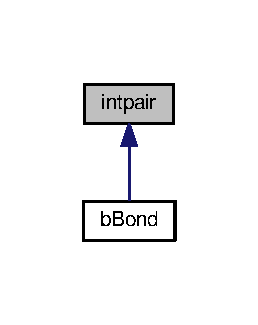
\includegraphics[width=124pt]{classintpair__inherit__graph}
\end{center}
\end{figure}
\subsection*{Public Member Functions}
\begin{DoxyCompactItemize}
\item 
{\bfseries intpair} (int inI, int inJ)\hypertarget{classintpair_ae531dd74d1f423a9ab00daee87f12ae0}{}\label{classintpair_ae531dd74d1f423a9ab00daee87f12ae0}

\item 
bool {\bfseries operator==} (const \hyperlink{classintpair}{intpair} $\ast$other)\hypertarget{classintpair_a652eac052b6323217efa7a40ead6184c}{}\label{classintpair_a652eac052b6323217efa7a40ead6184c}

\item 
bool {\bfseries operator!=} (const \hyperlink{classintpair}{intpair} $\ast$other)\hypertarget{classintpair_ae6d12c36f8eb9ceebbddcb89f3f1a98f}{}\label{classintpair_ae6d12c36f8eb9ceebbddcb89f3f1a98f}

\item 
bool {\bfseries is\+The\+Same\+As} (const \hyperlink{classintpair}{intpair} $\ast$other)\hypertarget{classintpair_a3580e37813128bfaf6a3df75bc379ba1}{}\label{classintpair_a3580e37813128bfaf6a3df75bc379ba1}

\item 
void {\bfseries swap} (void)\hypertarget{classintpair_a48e17868168d8f0d5dafd6234ae0f357}{}\label{classintpair_a48e17868168d8f0d5dafd6234ae0f357}

\item 
void {\bfseries dump} (void)\hypertarget{classintpair_a293807486458b365cfc44d68cd0c3577}{}\label{classintpair_a293807486458b365cfc44d68cd0c3577}

\item 
std\+::string {\bfseries get\+String} (void)\hypertarget{classintpair_a52590ac26c591ca5970c65aeabf46f50}{}\label{classintpair_a52590ac26c591ca5970c65aeabf46f50}

\end{DoxyCompactItemize}
\subsection*{Public Attributes}
\begin{DoxyCompactItemize}
\item 
int {\bfseries i}\hypertarget{classintpair_accfc85d2e86a853047c938ffe980e5cc}{}\label{classintpair_accfc85d2e86a853047c938ffe980e5cc}

\item 
int {\bfseries j}\hypertarget{classintpair_a631aa0b024f4050f8641a532ab169a56}{}\label{classintpair_a631aa0b024f4050f8641a532ab169a56}

\end{DoxyCompactItemize}


\subsection{Detailed Description}
Intpair Class is a two int vector used for connectivity definition in Molecule\+Reader. 

The documentation for this class was generated from the following files\+:\begin{DoxyCompactItemize}
\item 
include/gmolmodel/\hyperlink{bBond_8hpp}{b\+Bond.\+hpp}\item 
src/b\+Bond.\+cpp\end{DoxyCompactItemize}

\hypertarget{classIState}{}\section{I\+State Class Reference}
\label{classIState}\index{I\+State@{I\+State}}


Inheritance diagram for I\+State\+:\nopagebreak
\begin{figure}[H]
\begin{center}
\leavevmode
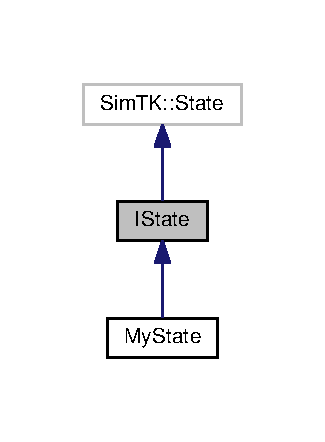
\includegraphics[width=156pt]{classIState__inherit__graph}
\end{center}
\end{figure}


Collaboration diagram for I\+State\+:\nopagebreak
\begin{figure}[H]
\begin{center}
\leavevmode
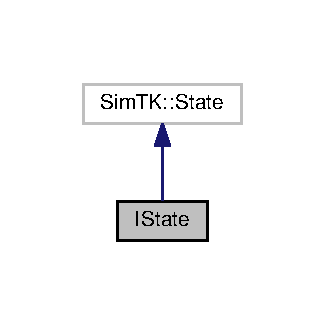
\includegraphics[width=156pt]{classIState__coll__graph}
\end{center}
\end{figure}
\subsection*{Public Member Functions}
\begin{DoxyCompactItemize}
\item 
virtual Sim\+T\+K\+::\+Vec3 {\bfseries get\+Cartesian} (int atom\+\_\+no)=0\hypertarget{classIState_ade2b2fe5193cede74f6c51830b6e92a6}{}\label{classIState_ade2b2fe5193cede74f6c51830b6e92a6}

\item 
virtual void {\bfseries upd\+Cartesian} (int atom\+\_\+no, Sim\+T\+K\+::\+Real x, Sim\+T\+K\+::\+Real y, Sim\+T\+K\+::\+Real z)=0\hypertarget{classIState_a71f8b4e24dae414fff178f3fa9dfbe69}{}\label{classIState_a71f8b4e24dae414fff178f3fa9dfbe69}

\item 
virtual void {\bfseries set\+Cartesian} (int atom\+\_\+no, Sim\+T\+K\+::\+Real x, Sim\+T\+K\+::\+Real y, Sim\+T\+K\+::\+Real z)=0\hypertarget{classIState_af1cba5a5867876864564e1abec9bfeb8}{}\label{classIState_af1cba5a5867876864564e1abec9bfeb8}

\end{DoxyCompactItemize}


The documentation for this class was generated from the following files\+:\begin{DoxyCompactItemize}
\item 
include/gmolmodel/I\+State.\+hpp\item 
src/I\+State.\+cpp\end{DoxyCompactItemize}

\hypertarget{classLAHMCSampler}{}\section{L\+A\+H\+M\+C\+Sampler Class Reference}
\label{classLAHMCSampler}\index{L\+A\+H\+M\+C\+Sampler@{L\+A\+H\+M\+C\+Sampler}}


{\ttfamily \#include $<$L\+A\+H\+M\+C\+Sampler.\+hpp$>$}



Inheritance diagram for L\+A\+H\+M\+C\+Sampler\+:\nopagebreak
\begin{figure}[H]
\begin{center}
\leavevmode
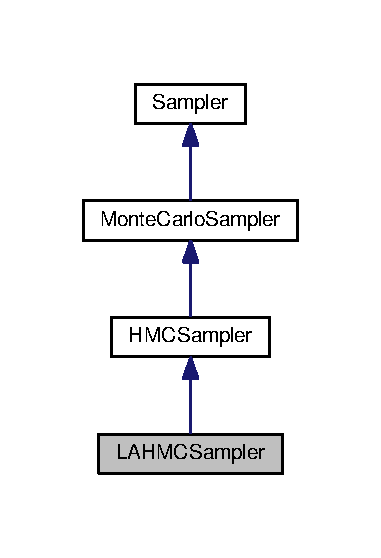
\includegraphics[width=183pt]{classLAHMCSampler__inherit__graph}
\end{center}
\end{figure}


Collaboration diagram for L\+A\+H\+M\+C\+Sampler\+:\nopagebreak
\begin{figure}[H]
\begin{center}
\leavevmode
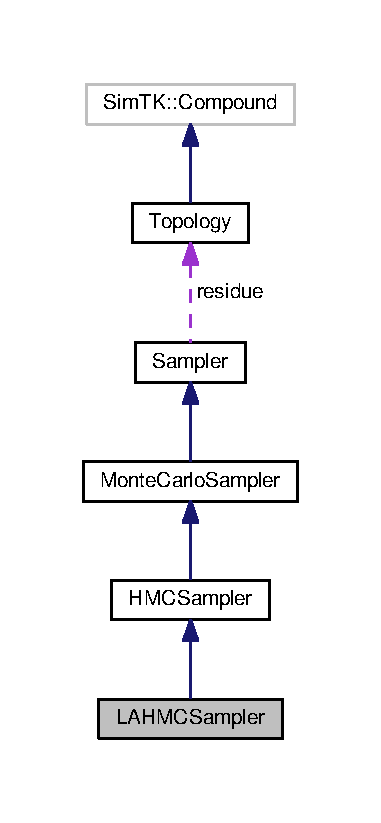
\includegraphics[width=183pt]{classLAHMCSampler__coll__graph}
\end{center}
\end{figure}
\subsection*{Public Member Functions}
\begin{DoxyCompactItemize}
\item 
\hyperlink{classLAHMCSampler_ac139a08ec777cd64d1166cf1b47d77cd}{L\+A\+H\+M\+C\+Sampler} (Sim\+T\+K\+::\+Compound\+System $\ast$arg\+Compound\+System, Sim\+T\+K\+::\+Simbody\+Matter\+Subsystem $\ast$arg\+Matter, std\+::vector$<$ \hyperlink{classTopology}{Topology} $\ast$ $>$ \&topologies, Sim\+T\+K\+::\+Du\+M\+M\+Force\+Field\+Subsystem $\ast$arg\+Dumm, Sim\+T\+K\+::\+General\+Force\+Subsystem $\ast$forces, Sim\+T\+K\+::\+Time\+Stepper $\ast$arg\+Time\+Stepper, unsigned int Kext)
\item 
virtual \hyperlink{classLAHMCSampler_ae6c15a0a2cd4dfc3f6873f5182182a19}{$\sim$\+L\+A\+H\+M\+C\+Sampler} ()
\item 
virtual void \hyperlink{classLAHMCSampler_a4cf1b6d5169675be6687b2eef7e14c61}{initialize} (Sim\+T\+K\+::\+State \&advanced)
\item 
virtual void \hyperlink{classLAHMCSampler_a11e1f9bee0627776686d546efba9d2e6}{reinitialize} (Sim\+T\+K\+::\+State \&advanced)
\item 
void \hyperlink{classLAHMCSampler_a95a06df36c18ea2cad5bea8a7e2b5926}{store\+Old\+Configuration\+And\+Potential\+Energies} (Sim\+T\+K\+::\+State \&some\+State)
\item 
void \hyperlink{classLAHMCSampler_a647e291c4044ca37a4bff16753b76416}{initialize\+Velocities} (Sim\+T\+K\+::\+State \&some\+State)
\item 
void \hyperlink{classLAHMCSampler_a230ea62c24f9873aee71b4fe50049385}{calc\+Proposed\+Kinetic\+And\+Total\+Energy} (Sim\+T\+K\+::\+State \&some\+State)
\item 
void \hyperlink{classLAHMCSampler_a2759e95ec5a15a447a20b59f3df28ef8}{integrate\+Trajectory} (Sim\+T\+K\+::\+State \&some\+State)
\item 
void \hyperlink{classLAHMCSampler_ae90a88374791995683313425966a4b7a}{calc\+New\+Configuration\+And\+Energies} (Sim\+T\+K\+::\+State \&some\+State, int k)
\item 
void {\bfseries reset\+C\+Matrices} (void)\hypertarget{classLAHMCSampler_ae148d78b17cafbacd047dc86a64556d4}{}\label{classLAHMCSampler_ae148d78b17cafbacd047dc86a64556d4}

\item 
Sim\+T\+K\+::\+Matrix {\bfseries extract\+From\+Top} (Sim\+T\+K\+::\+Matrix M, int row\+Cut, int col\+Cut)\hypertarget{classLAHMCSampler_aafbbd957069afd2ef1132414182f869e}{}\label{classLAHMCSampler_aafbbd957069afd2ef1132414182f869e}

\item 
void {\bfseries inject\+From\+Top} (const std\+::vector$<$ Sim\+T\+K\+::\+Real $>$ \&src, std\+::vector$<$ Sim\+T\+K\+::\+Real $>$ \&dest)\hypertarget{classLAHMCSampler_aedd525ca52d9d2a785b851a1480bb0db}{}\label{classLAHMCSampler_aedd525ca52d9d2a785b851a1480bb0db}

\item 
void {\bfseries inject\+From\+Top} (const Sim\+T\+K\+::\+Matrix \&src, Sim\+T\+K\+::\+Matrix \&dest)\hypertarget{classLAHMCSampler_ab0e8be72dae629b8de3e17efe1eea6e8}{}\label{classLAHMCSampler_ab0e8be72dae629b8de3e17efe1eea6e8}

\item 
Sim\+T\+K\+::\+Matrix {\bfseries reverse\+Matrix} (Sim\+T\+K\+::\+Matrix M)\hypertarget{classLAHMCSampler_a6aefd73ab099cdc45a3c999a35871ea0}{}\label{classLAHMCSampler_a6aefd73ab099cdc45a3c999a35871ea0}

\item 
void {\bfseries set\+C\+Entry} (int i, int j, Sim\+T\+K\+::\+Real entry)\hypertarget{classLAHMCSampler_a100856ce2d65a5c3af4a4fa23d03cec2}{}\label{classLAHMCSampler_a100856ce2d65a5c3af4a4fa23d03cec2}

\item 
void {\bfseries set\+Ctau\+Entry} (int i, int j, Sim\+T\+K\+::\+Real entry)\hypertarget{classLAHMCSampler_a9879e684da63e3b2e4a1901358cd6c1e}{}\label{classLAHMCSampler_a9879e684da63e3b2e4a1901358cd6c1e}

\item 
void {\bfseries C\+\_\+to\+\_\+\+Ctau\+\_\+\+Indeces} (int C\+\_\+i, int C\+\_\+j, int \&Ctau\+\_\+i, int \&Ctau\+\_\+j, int curr\+Size)\hypertarget{classLAHMCSampler_a19eb270fc5a18dfd3912f4eb3e8f8c0c}{}\label{classLAHMCSampler_a19eb270fc5a18dfd3912f4eb3e8f8c0c}

\item 
void {\bfseries Ctau\+\_\+to\+\_\+\+C\+\_\+\+Indeces} (int Ctau\+\_\+i, int Ctau\+\_\+j, int \&C\+\_\+i, int \&C\+\_\+j, int curr\+Size)\hypertarget{classLAHMCSampler_a665643ec6077e31d00487df685bb1595}{}\label{classLAHMCSampler_a665643ec6077e31d00487df685bb1595}

\item 
Sim\+T\+K\+::\+Real \hyperlink{classLAHMCSampler_a6a3e967f12c5c64dda41c395bf755e6b}{M\+H\+Accept\+Probability} (Sim\+T\+K\+::\+State \&some\+State, Sim\+T\+K\+::\+Real E\+\_\+o, Sim\+T\+K\+::\+Real E\+\_\+n)
\item 
Sim\+T\+K\+::\+Matrix \& {\bfseries leap\+\_\+prob\+\_\+recurse\+\_\+hard} (Sim\+T\+K\+::\+State \&some\+State, std\+::vector$<$ Sim\+T\+K\+::\+Real $>$ etot\+\_\+ns\+\_\+loc, Sim\+T\+K\+::\+Matrix \&C\+C\+\_\+loc)\hypertarget{classLAHMCSampler_ad41e507cc48b82d7a6b924879a39dec8}{}\label{classLAHMCSampler_ad41e507cc48b82d7a6b924879a39dec8}

\item 
void \hyperlink{classLAHMCSampler_ae7a0d2db9791c6e6947d8273b90f95b8}{set\+Set\+Configuration\+And\+Energies\+To\+New} (Sim\+T\+K\+::\+State \&some\+State)
\item 
void \hyperlink{classLAHMCSampler_aedb4b87feaaa20c036c908c9e9868b41}{propose} (Sim\+T\+K\+::\+State \&some\+State)
\item 
void \hyperlink{classLAHMCSampler_ace1c39b2b136a63d4f00bb5fcd5508c9}{update} (Sim\+T\+K\+::\+State \&some\+State)
\item 
virtual bool \hyperlink{classLAHMCSampler_a0baac57ec1fe8d795a6fea65acdf86ed}{acc\+Rej\+Step} (Sim\+T\+K\+::\+State \&some\+State)
\item 
bool {\bfseries sample\+\_\+iteration} (Sim\+T\+K\+::\+State \&some\+State)\hypertarget{classLAHMCSampler_a0c41a55a68bd21dd21d12c242880495b}{}\label{classLAHMCSampler_a0c41a55a68bd21dd21d12c242880495b}

\item 
Sim\+T\+K\+::\+Real \hyperlink{classLAHMCSampler_a45b90c6c7fb2aa0058190de36049f52e}{get\+Proposed\+KE} (void)
\item 
Sim\+T\+K\+::\+Real \hyperlink{classLAHMCSampler_afa344b5c330421f52c67b7f5f0eee39b}{get\+Last\+Accepted\+KE} (void)
\item 
void \hyperlink{classLAHMCSampler_a784d850d71f9bd99db8b487ed4d8d95e}{set\+Proposed\+KE} (Sim\+T\+K\+::\+Real)
\item 
void \hyperlink{classLAHMCSampler_aa5541db7afb121ab861691c78cf3ed1e}{set\+Last\+Accepted\+KE} (Sim\+T\+K\+::\+Real)
\item 
int {\bfseries get\+M\+D\+Steps\+Per\+Sample} () const \hypertarget{classLAHMCSampler_a21960c0eb41e0f5770889ef746b2d0d3}{}\label{classLAHMCSampler_a21960c0eb41e0f5770889ef746b2d0d3}

\item 
void {\bfseries set\+M\+D\+Steps\+Per\+Sample} (int md\+Steps\+Per\+Sample)\hypertarget{classLAHMCSampler_a23c87fbcec2e0eb55d80fdd46b3b222d}{}\label{classLAHMCSampler_a23c87fbcec2e0eb55d80fdd46b3b222d}

\item 
void \hyperlink{classLAHMCSampler_af62872905cee7ce8de045115a269a670}{Print\+Detailed\+Energy\+Info} (Sim\+T\+K\+::\+State \&some\+State)
\end{DoxyCompactItemize}
\subsection*{Protected Attributes}
\begin{DoxyCompactItemize}
\item 
int {\bfseries K}\hypertarget{classLAHMCSampler_a6fb2d8a9f06d161c5a837c8b912f70fa}{}\label{classLAHMCSampler_a6fb2d8a9f06d161c5a837c8b912f70fa}

\item 
std\+::vector$<$ Sim\+T\+K\+::\+Real $>$ {\bfseries pe\+\_\+ns}\hypertarget{classLAHMCSampler_a5cb7b53a7c914eeea1782a571197b835}{}\label{classLAHMCSampler_a5cb7b53a7c914eeea1782a571197b835}

\item 
std\+::vector$<$ Sim\+T\+K\+::\+Real $>$ {\bfseries fix\+\_\+ns}\hypertarget{classLAHMCSampler_a6257e83ae48c3b849f96d0796bd431e9}{}\label{classLAHMCSampler_a6257e83ae48c3b849f96d0796bd431e9}

\item 
std\+::vector$<$ Sim\+T\+K\+::\+Real $>$ {\bfseries log\+Sine\+Sqr\+Gamma2\+\_\+ns}\hypertarget{classLAHMCSampler_add11d937ef56d4bbf0970ac76e958535}{}\label{classLAHMCSampler_add11d937ef56d4bbf0970ac76e958535}

\item 
std\+::vector$<$ Sim\+T\+K\+::\+Real $>$ {\bfseries ke\+\_\+ns}\hypertarget{classLAHMCSampler_a55d8f1378d5200107fdb8f3abc43a354}{}\label{classLAHMCSampler_a55d8f1378d5200107fdb8f3abc43a354}

\item 
std\+::vector$<$ Sim\+T\+K\+::\+Real $>$ {\bfseries etot\+\_\+ns}\hypertarget{classLAHMCSampler_a6992320ce81d608b84fdea4386b43fbd}{}\label{classLAHMCSampler_a6992320ce81d608b84fdea4386b43fbd}

\item 
Sim\+T\+K\+::\+Matrix {\bfseries C}\hypertarget{classLAHMCSampler_a73138f7fd34e877e393f0409afeffbe1}{}\label{classLAHMCSampler_a73138f7fd34e877e393f0409afeffbe1}

\item 
Sim\+T\+K\+::\+Matrix {\bfseries Ctau}\hypertarget{classLAHMCSampler_a7e9132c332389e404a409d4abb75125b}{}\label{classLAHMCSampler_a7e9132c332389e404a409d4abb75125b}

\item 
Sim\+T\+K\+::\+Matrix {\bfseries P}\hypertarget{classLAHMCSampler_a3a815eae4e31199eae811722b00a6306}{}\label{classLAHMCSampler_a3a815eae4e31199eae811722b00a6306}

\item 
Sim\+T\+K\+::\+Matrix {\bfseries CC}\hypertarget{classLAHMCSampler_ae6bab0d320d3b9d90e26b7cbbb9ace44}{}\label{classLAHMCSampler_ae6bab0d320d3b9d90e26b7cbbb9ace44}

\end{DoxyCompactItemize}
\subsection*{Friends}
\begin{DoxyCompactItemize}
\item 
class {\bfseries Context}\hypertarget{classLAHMCSampler_ac26c806e60ca4a0547680edb68f6e39b}{}\label{classLAHMCSampler_ac26c806e60ca4a0547680edb68f6e39b}

\end{DoxyCompactItemize}
\subsection*{Additional Inherited Members}


\subsection{Detailed Description}
A Generalized Coordiantes Hamiltonian Monte Carlo sampler as described in J Chem Theory Comput. 2017 Oct 10;13(10)\+:4649-\/4659. In short it consists of the following steps\+:
\begin{DoxyEnumerate}
\item Initialize velocities from a random normal distribution with a covariance of kT sqrt(\+M) where M is the mass matrix tensor.
\item Propagate the trial trajectory using a symplectic integrator provided by Simbody
\item An acception-\/rejection step which includes the Fixman potential if needed. Step 1 and 2 are implemented in the fuction propose. Step 3 is implemented in the function update. 
\end{DoxyEnumerate}

\subsection{Constructor \& Destructor Documentation}
\index{L\+A\+H\+M\+C\+Sampler@{L\+A\+H\+M\+C\+Sampler}!L\+A\+H\+M\+C\+Sampler@{L\+A\+H\+M\+C\+Sampler}}
\index{L\+A\+H\+M\+C\+Sampler@{L\+A\+H\+M\+C\+Sampler}!L\+A\+H\+M\+C\+Sampler@{L\+A\+H\+M\+C\+Sampler}}
\subsubsection[{\texorpdfstring{L\+A\+H\+M\+C\+Sampler(\+Sim\+T\+K\+::\+Compound\+System $\ast$arg\+Compound\+System, Sim\+T\+K\+::\+Simbody\+Matter\+Subsystem $\ast$arg\+Matter, std\+::vector$<$ Topology $\ast$ $>$ \&topologies, Sim\+T\+K\+::\+Du\+M\+M\+Force\+Field\+Subsystem $\ast$arg\+Dumm, Sim\+T\+K\+::\+General\+Force\+Subsystem $\ast$forces, Sim\+T\+K\+::\+Time\+Stepper $\ast$arg\+Time\+Stepper, unsigned int Kext)}{LAHMCSampler(SimTK::CompoundSystem *argCompoundSystem, SimTK::SimbodyMatterSubsystem *argMatter, std::vector< Topology * > &topologies, SimTK::DuMMForceFieldSubsystem *argDumm, SimTK::GeneralForceSubsystem *forces, SimTK::TimeStepper *argTimeStepper, unsigned int Kext)}}]{\setlength{\rightskip}{0pt plus 5cm}L\+A\+H\+M\+C\+Sampler\+::\+L\+A\+H\+M\+C\+Sampler (
\begin{DoxyParamCaption}
\item[{Sim\+T\+K\+::\+Compound\+System $\ast$}]{arg\+Compound\+System, }
\item[{Sim\+T\+K\+::\+Simbody\+Matter\+Subsystem $\ast$}]{arg\+Matter, }
\item[{std\+::vector$<$ {\bf Topology} $\ast$ $>$ \&}]{topologies, }
\item[{Sim\+T\+K\+::\+Du\+M\+M\+Force\+Field\+Subsystem $\ast$}]{arg\+Dumm, }
\item[{Sim\+T\+K\+::\+General\+Force\+Subsystem $\ast$}]{forces, }
\item[{Sim\+T\+K\+::\+Time\+Stepper $\ast$}]{arg\+Time\+Stepper, }
\item[{unsigned int}]{Kext}
\end{DoxyParamCaption}
)}\hypertarget{classLAHMCSampler_ac139a08ec777cd64d1166cf1b47d77cd}{}\label{classLAHMCSampler_ac139a08ec777cd64d1166cf1b47d77cd}
Constructor \index{L\+A\+H\+M\+C\+Sampler@{L\+A\+H\+M\+C\+Sampler}!````~L\+A\+H\+M\+C\+Sampler@{$\sim$\+L\+A\+H\+M\+C\+Sampler}}
\index{````~L\+A\+H\+M\+C\+Sampler@{$\sim$\+L\+A\+H\+M\+C\+Sampler}!L\+A\+H\+M\+C\+Sampler@{L\+A\+H\+M\+C\+Sampler}}
\subsubsection[{\texorpdfstring{$\sim$\+L\+A\+H\+M\+C\+Sampler()}{~LAHMCSampler()}}]{\setlength{\rightskip}{0pt plus 5cm}L\+A\+H\+M\+C\+Sampler\+::$\sim$\+L\+A\+H\+M\+C\+Sampler (
\begin{DoxyParamCaption}
{}
\end{DoxyParamCaption}
)\hspace{0.3cm}{\ttfamily [virtual]}}\hypertarget{classLAHMCSampler_ae6c15a0a2cd4dfc3f6873f5182182a19}{}\label{classLAHMCSampler_ae6c15a0a2cd4dfc3f6873f5182182a19}
Destructor 

\subsection{Member Function Documentation}
\index{L\+A\+H\+M\+C\+Sampler@{L\+A\+H\+M\+C\+Sampler}!acc\+Rej\+Step@{acc\+Rej\+Step}}
\index{acc\+Rej\+Step@{acc\+Rej\+Step}!L\+A\+H\+M\+C\+Sampler@{L\+A\+H\+M\+C\+Sampler}}
\subsubsection[{\texorpdfstring{acc\+Rej\+Step(\+Sim\+T\+K\+::\+State \&some\+State)}{accRejStep(SimTK::State &someState)}}]{\setlength{\rightskip}{0pt plus 5cm}bool L\+A\+H\+M\+C\+Sampler\+::acc\+Rej\+Step (
\begin{DoxyParamCaption}
\item[{Sim\+T\+K\+::\+State \&}]{some\+State}
\end{DoxyParamCaption}
)\hspace{0.3cm}{\ttfamily [virtual]}}\hypertarget{classLAHMCSampler_a0baac57ec1fe8d795a6fea65acdf86ed}{}\label{classLAHMCSampler_a0baac57ec1fe8d795a6fea65acdf86ed}
Accetion rejection step

Acception rejection step 

Reimplemented from \hyperlink{classHMCSampler_af5e87c855b8888196a9f2ad87bb9f824}{H\+M\+C\+Sampler}.

\index{L\+A\+H\+M\+C\+Sampler@{L\+A\+H\+M\+C\+Sampler}!calc\+New\+Configuration\+And\+Energies@{calc\+New\+Configuration\+And\+Energies}}
\index{calc\+New\+Configuration\+And\+Energies@{calc\+New\+Configuration\+And\+Energies}!L\+A\+H\+M\+C\+Sampler@{L\+A\+H\+M\+C\+Sampler}}
\subsubsection[{\texorpdfstring{calc\+New\+Configuration\+And\+Energies(\+Sim\+T\+K\+::\+State \&some\+State, int k)}{calcNewConfigurationAndEnergies(SimTK::State &someState, int k)}}]{\setlength{\rightskip}{0pt plus 5cm}void L\+A\+H\+M\+C\+Sampler\+::calc\+New\+Configuration\+And\+Energies (
\begin{DoxyParamCaption}
\item[{Sim\+T\+K\+::\+State \&}]{some\+State, }
\item[{int}]{k}
\end{DoxyParamCaption}
)}\hypertarget{classLAHMCSampler_ae90a88374791995683313425966a4b7a}{}\label{classLAHMCSampler_ae90a88374791995683313425966a4b7a}
Store new configuration and energy terms \index{L\+A\+H\+M\+C\+Sampler@{L\+A\+H\+M\+C\+Sampler}!calc\+Proposed\+Kinetic\+And\+Total\+Energy@{calc\+Proposed\+Kinetic\+And\+Total\+Energy}}
\index{calc\+Proposed\+Kinetic\+And\+Total\+Energy@{calc\+Proposed\+Kinetic\+And\+Total\+Energy}!L\+A\+H\+M\+C\+Sampler@{L\+A\+H\+M\+C\+Sampler}}
\subsubsection[{\texorpdfstring{calc\+Proposed\+Kinetic\+And\+Total\+Energy(\+Sim\+T\+K\+::\+State \&some\+State)}{calcProposedKineticAndTotalEnergy(SimTK::State &someState)}}]{\setlength{\rightskip}{0pt plus 5cm}void L\+A\+H\+M\+C\+Sampler\+::calc\+Proposed\+Kinetic\+And\+Total\+Energy (
\begin{DoxyParamCaption}
\item[{Sim\+T\+K\+::\+State \&}]{some\+State}
\end{DoxyParamCaption}
)\hspace{0.3cm}{\ttfamily [virtual]}}\hypertarget{classLAHMCSampler_a230ea62c24f9873aee71b4fe50049385}{}\label{classLAHMCSampler_a230ea62c24f9873aee71b4fe50049385}
Store the proposed energies 

Reimplemented from \hyperlink{classHMCSampler_a492f12a031effba381c409052ab734e7}{H\+M\+C\+Sampler}.

\index{L\+A\+H\+M\+C\+Sampler@{L\+A\+H\+M\+C\+Sampler}!get\+Last\+Accepted\+KE@{get\+Last\+Accepted\+KE}}
\index{get\+Last\+Accepted\+KE@{get\+Last\+Accepted\+KE}!L\+A\+H\+M\+C\+Sampler@{L\+A\+H\+M\+C\+Sampler}}
\subsubsection[{\texorpdfstring{get\+Last\+Accepted\+K\+E(void)}{getLastAcceptedKE(void)}}]{\setlength{\rightskip}{0pt plus 5cm}Sim\+T\+K\+::\+Real L\+A\+H\+M\+C\+Sampler\+::get\+Last\+Accepted\+KE (
\begin{DoxyParamCaption}
\item[{void}]{}
\end{DoxyParamCaption}
)\hspace{0.3cm}{\ttfamily [inline]}}\hypertarget{classLAHMCSampler_afa344b5c330421f52c67b7f5f0eee39b}{}\label{classLAHMCSampler_afa344b5c330421f52c67b7f5f0eee39b}
Get the stored kinetic energy. This is set rightafter a move is accepted. It\textquotesingle{}s a component of the total energy stored. \index{L\+A\+H\+M\+C\+Sampler@{L\+A\+H\+M\+C\+Sampler}!get\+Proposed\+KE@{get\+Proposed\+KE}}
\index{get\+Proposed\+KE@{get\+Proposed\+KE}!L\+A\+H\+M\+C\+Sampler@{L\+A\+H\+M\+C\+Sampler}}
\subsubsection[{\texorpdfstring{get\+Proposed\+K\+E(void)}{getProposedKE(void)}}]{\setlength{\rightskip}{0pt plus 5cm}Sim\+T\+K\+::\+Real L\+A\+H\+M\+C\+Sampler\+::get\+Proposed\+KE (
\begin{DoxyParamCaption}
\item[{void}]{}
\end{DoxyParamCaption}
)\hspace{0.3cm}{\ttfamily [inline]}}\hypertarget{classLAHMCSampler_a45b90c6c7fb2aa0058190de36049f52e}{}\label{classLAHMCSampler_a45b90c6c7fb2aa0058190de36049f52e}
Modifies Q randomly Get the proposed kinetic energy. This is set right after velocities are initialized. \index{L\+A\+H\+M\+C\+Sampler@{L\+A\+H\+M\+C\+Sampler}!initialize@{initialize}}
\index{initialize@{initialize}!L\+A\+H\+M\+C\+Sampler@{L\+A\+H\+M\+C\+Sampler}}
\subsubsection[{\texorpdfstring{initialize(\+Sim\+T\+K\+::\+State \&advanced)}{initialize(SimTK::State &advanced)}}]{\setlength{\rightskip}{0pt plus 5cm}void L\+A\+H\+M\+C\+Sampler\+::initialize (
\begin{DoxyParamCaption}
\item[{Sim\+T\+K\+::\+State \&}]{some\+State}
\end{DoxyParamCaption}
)\hspace{0.3cm}{\ttfamily [virtual]}}\hypertarget{classLAHMCSampler_a4cf1b6d5169675be6687b2eef7e14c61}{}\label{classLAHMCSampler_a4cf1b6d5169675be6687b2eef7e14c61}
Calculate O(n2) the square root of the mass matrix inverse denoted by Jain l$\ast$ = \mbox{[}I -\/\+J\+PsiK\mbox{]}$\ast$sqrt(D) (adjoint of l). This is lower triangular Calculate O(n2) the square root of the mass matrix inverse denoted by Jain l = sqrt(\+D) $\ast$ \mbox{[}I -\/\+J\+PsiK\mbox{]}. This is upper triangular Calculate sqrt(\+M) using Eigen. For debug purposes. Seed the random number generator. Set simulation temperature, velocities to desired temperature, variables that store the configuration and variables that store the energies, both needed for the acception-\/rejection step. Also realize velocities and initialize the timestepper.

Get/set the Time\+Stepper that manages the integrator Seed the random number generator. Set simulation temperature, velocities to desired temperature, variables that store the configuration and variables that store the energies, both needed for the acception-\/rejection step. Also realize velocities and initialize the timestepper. 

Reimplemented from \hyperlink{classHMCSampler_ad878471d3e5222758b2544f76affd79a}{H\+M\+C\+Sampler}.

\index{L\+A\+H\+M\+C\+Sampler@{L\+A\+H\+M\+C\+Sampler}!initialize\+Velocities@{initialize\+Velocities}}
\index{initialize\+Velocities@{initialize\+Velocities}!L\+A\+H\+M\+C\+Sampler@{L\+A\+H\+M\+C\+Sampler}}
\subsubsection[{\texorpdfstring{initialize\+Velocities(\+Sim\+T\+K\+::\+State \&some\+State)}{initializeVelocities(SimTK::State &someState)}}]{\setlength{\rightskip}{0pt plus 5cm}void L\+A\+H\+M\+C\+Sampler\+::initialize\+Velocities (
\begin{DoxyParamCaption}
\item[{Sim\+T\+K\+::\+State \&}]{some\+State}
\end{DoxyParamCaption}
)\hspace{0.3cm}{\ttfamily [virtual]}}\hypertarget{classLAHMCSampler_a647e291c4044ca37a4bff16753b76416}{}\label{classLAHMCSampler_a647e291c4044ca37a4bff16753b76416}
Initialize velocities according to the Maxwell-\/\+Boltzmann distribution. Coresponds to R operator in L\+A\+H\+MC 

Reimplemented from \hyperlink{classHMCSampler_ae38d8206113980732d4adced081c50fd}{H\+M\+C\+Sampler}.

\index{L\+A\+H\+M\+C\+Sampler@{L\+A\+H\+M\+C\+Sampler}!integrate\+Trajectory@{integrate\+Trajectory}}
\index{integrate\+Trajectory@{integrate\+Trajectory}!L\+A\+H\+M\+C\+Sampler@{L\+A\+H\+M\+C\+Sampler}}
\subsubsection[{\texorpdfstring{integrate\+Trajectory(\+Sim\+T\+K\+::\+State \&some\+State)}{integrateTrajectory(SimTK::State &someState)}}]{\setlength{\rightskip}{0pt plus 5cm}void L\+A\+H\+M\+C\+Sampler\+::integrate\+Trajectory (
\begin{DoxyParamCaption}
\item[{Sim\+T\+K\+::\+State \&}]{some\+State}
\end{DoxyParamCaption}
)\hspace{0.3cm}{\ttfamily [virtual]}}\hypertarget{classLAHMCSampler_a2759e95ec5a15a447a20b59f3df28ef8}{}\label{classLAHMCSampler_a2759e95ec5a15a447a20b59f3df28ef8}
Apply the L operator 

Reimplemented from \hyperlink{classHMCSampler_ab3b4de64be2a10193e274f05788b5ca5}{H\+M\+C\+Sampler}.

\index{L\+A\+H\+M\+C\+Sampler@{L\+A\+H\+M\+C\+Sampler}!M\+H\+Accept\+Probability@{M\+H\+Accept\+Probability}}
\index{M\+H\+Accept\+Probability@{M\+H\+Accept\+Probability}!L\+A\+H\+M\+C\+Sampler@{L\+A\+H\+M\+C\+Sampler}}
\subsubsection[{\texorpdfstring{M\+H\+Accept\+Probability(\+Sim\+T\+K\+::\+State \&some\+State, Sim\+T\+K\+::\+Real E\+\_\+o, Sim\+T\+K\+::\+Real E\+\_\+n)}{MHAcceptProbability(SimTK::State &someState, SimTK::Real E_o, SimTK::Real E_n)}}]{\setlength{\rightskip}{0pt plus 5cm}Sim\+T\+K\+::\+Real L\+A\+H\+M\+C\+Sampler\+::\+M\+H\+Accept\+Probability (
\begin{DoxyParamCaption}
\item[{Sim\+T\+K\+::\+State \&}]{some\+State, }
\item[{Sim\+T\+K\+::\+Real}]{arg\+Etot\+\_\+proposed, }
\item[{Sim\+T\+K\+::\+Real}]{arg\+Etot\+\_\+n}
\end{DoxyParamCaption}
)\hspace{0.3cm}{\ttfamily [virtual]}}\hypertarget{classLAHMCSampler_a6a3e967f12c5c64dda41c395bf755e6b}{}\label{classLAHMCSampler_a6a3e967f12c5c64dda41c395bf755e6b}
Metropolis-\/\+Hastings acceptance probability 

Reimplemented from \hyperlink{classHMCSampler_a7fee5ad6d531c32235db96c4b95f1eca}{H\+M\+C\+Sampler}.

\index{L\+A\+H\+M\+C\+Sampler@{L\+A\+H\+M\+C\+Sampler}!Print\+Detailed\+Energy\+Info@{Print\+Detailed\+Energy\+Info}}
\index{Print\+Detailed\+Energy\+Info@{Print\+Detailed\+Energy\+Info}!L\+A\+H\+M\+C\+Sampler@{L\+A\+H\+M\+C\+Sampler}}
\subsubsection[{\texorpdfstring{Print\+Detailed\+Energy\+Info(\+Sim\+T\+K\+::\+State \&some\+State)}{PrintDetailedEnergyInfo(SimTK::State &someState)}}]{\setlength{\rightskip}{0pt plus 5cm}void L\+A\+H\+M\+C\+Sampler\+::\+Print\+Detailed\+Energy\+Info (
\begin{DoxyParamCaption}
\item[{Sim\+T\+K\+::\+State \&}]{some\+State}
\end{DoxyParamCaption}
)}\hypertarget{classLAHMCSampler_af62872905cee7ce8de045115a269a670}{}\label{classLAHMCSampler_af62872905cee7ce8de045115a269a670}
Print detailed energy information \index{L\+A\+H\+M\+C\+Sampler@{L\+A\+H\+M\+C\+Sampler}!propose@{propose}}
\index{propose@{propose}!L\+A\+H\+M\+C\+Sampler@{L\+A\+H\+M\+C\+Sampler}}
\subsubsection[{\texorpdfstring{propose(\+Sim\+T\+K\+::\+State \&some\+State)}{propose(SimTK::State &someState)}}]{\setlength{\rightskip}{0pt plus 5cm}void L\+A\+H\+M\+C\+Sampler\+::propose (
\begin{DoxyParamCaption}
\item[{Sim\+T\+K\+::\+State \&}]{some\+State}
\end{DoxyParamCaption}
)\hspace{0.3cm}{\ttfamily [virtual]}}\hypertarget{classLAHMCSampler_aedb4b87feaaa20c036c908c9e9868b41}{}\label{classLAHMCSampler_aedb4b87feaaa20c036c908c9e9868b41}
It implements the proposal move in the Hamiltonian Monte Carlo algorithm. It essentially propagates the trajectory after it stores the configuration and energies. T\+O\+DO\+: break in two functions\+: initialize\+Velocities and propagate/integrate 

Reimplemented from \hyperlink{classHMCSampler_aa36ab4482bbb6295658e8fe6a49c9e4f}{H\+M\+C\+Sampler}.

\index{L\+A\+H\+M\+C\+Sampler@{L\+A\+H\+M\+C\+Sampler}!reinitialize@{reinitialize}}
\index{reinitialize@{reinitialize}!L\+A\+H\+M\+C\+Sampler@{L\+A\+H\+M\+C\+Sampler}}
\subsubsection[{\texorpdfstring{reinitialize(\+Sim\+T\+K\+::\+State \&advanced)}{reinitialize(SimTK::State &advanced)}}]{\setlength{\rightskip}{0pt plus 5cm}void L\+A\+H\+M\+C\+Sampler\+::reinitialize (
\begin{DoxyParamCaption}
\item[{Sim\+T\+K\+::\+State \&}]{some\+State}
\end{DoxyParamCaption}
)\hspace{0.3cm}{\ttfamily [virtual]}}\hypertarget{classLAHMCSampler_a11e1f9bee0627776686d546efba9d2e6}{}\label{classLAHMCSampler_a11e1f9bee0627776686d546efba9d2e6}
Same as initialize 

Reimplemented from \hyperlink{classHMCSampler_a43a302d87e149bfa893a5952ec20941f}{H\+M\+C\+Sampler}.

\index{L\+A\+H\+M\+C\+Sampler@{L\+A\+H\+M\+C\+Sampler}!set\+Last\+Accepted\+KE@{set\+Last\+Accepted\+KE}}
\index{set\+Last\+Accepted\+KE@{set\+Last\+Accepted\+KE}!L\+A\+H\+M\+C\+Sampler@{L\+A\+H\+M\+C\+Sampler}}
\subsubsection[{\texorpdfstring{set\+Last\+Accepted\+K\+E(\+Sim\+T\+K\+::\+Real)}{setLastAcceptedKE(SimTK::Real)}}]{\setlength{\rightskip}{0pt plus 5cm}void L\+A\+H\+M\+C\+Sampler\+::set\+Last\+Accepted\+KE (
\begin{DoxyParamCaption}
\item[{Sim\+T\+K\+::\+Real}]{inp\+KE}
\end{DoxyParamCaption}
)}\hypertarget{classLAHMCSampler_aa5541db7afb121ab861691c78cf3ed1e}{}\label{classLAHMCSampler_aa5541db7afb121ab861691c78cf3ed1e}
Stores the accepted kinetic energy. This should be set right after a move is accepted. It\textquotesingle{}s a component of the total energy stored.

Calculate sqrt(\+M) using Eigen. For debug purposes. Calculate O(n2) the square root of the mass matrix inverse denoted by Jain l = sqrt(\+D) $\ast$ \mbox{[}I -\/\+J\+PsiK\mbox{]}. This is upper triangular matrix and it is computed multipling a set of orthonormal vectors with the sqrt(\+M\+Inv). Calculate O(n2) the square root of the mass matrix inverse denoted by Jain l$\ast$ = \mbox{[}I -\/\+J\+PsiK\mbox{]}$\ast$sqrt(D) (adjoint of l). This is lower triangular matrix and it is computed by multipling a set of orthonormal vectors with the sqrt(\+M\+Inv) and transpose it. Stores the accepted kinetic energy. This should be set right after a move is accepted. It\textquotesingle{}s a component of the total energy stored. \index{L\+A\+H\+M\+C\+Sampler@{L\+A\+H\+M\+C\+Sampler}!set\+Proposed\+KE@{set\+Proposed\+KE}}
\index{set\+Proposed\+KE@{set\+Proposed\+KE}!L\+A\+H\+M\+C\+Sampler@{L\+A\+H\+M\+C\+Sampler}}
\subsubsection[{\texorpdfstring{set\+Proposed\+K\+E(\+Sim\+T\+K\+::\+Real)}{setProposedKE(SimTK::Real)}}]{\setlength{\rightskip}{0pt plus 5cm}void L\+A\+H\+M\+C\+Sampler\+::set\+Proposed\+KE (
\begin{DoxyParamCaption}
\item[{Sim\+T\+K\+::\+Real}]{inp\+KE}
\end{DoxyParamCaption}
)}\hypertarget{classLAHMCSampler_a784d850d71f9bd99db8b487ed4d8d95e}{}\label{classLAHMCSampler_a784d850d71f9bd99db8b487ed4d8d95e}
Sets the proposed kinetic energy before the proposal. This should be set right after the velocities are initialized. \index{L\+A\+H\+M\+C\+Sampler@{L\+A\+H\+M\+C\+Sampler}!set\+Set\+Configuration\+And\+Energies\+To\+New@{set\+Set\+Configuration\+And\+Energies\+To\+New}}
\index{set\+Set\+Configuration\+And\+Energies\+To\+New@{set\+Set\+Configuration\+And\+Energies\+To\+New}!L\+A\+H\+M\+C\+Sampler@{L\+A\+H\+M\+C\+Sampler}}
\subsubsection[{\texorpdfstring{set\+Set\+Configuration\+And\+Energies\+To\+New(\+Sim\+T\+K\+::\+State \&some\+State)}{setSetConfigurationAndEnergiesToNew(SimTK::State &someState)}}]{\setlength{\rightskip}{0pt plus 5cm}void L\+A\+H\+M\+C\+Sampler\+::set\+Set\+Configuration\+And\+Energies\+To\+New (
\begin{DoxyParamCaption}
\item[{Sim\+T\+K\+::\+State \&}]{some\+State}
\end{DoxyParamCaption}
)\hspace{0.3cm}{\ttfamily [virtual]}}\hypertarget{classLAHMCSampler_ae7a0d2db9791c6e6947d8273b90f95b8}{}\label{classLAHMCSampler_ae7a0d2db9791c6e6947d8273b90f95b8}
Store new configuration and energy terms 

Reimplemented from \hyperlink{classHMCSampler_a4deb485f9bfc31d64f6ada06536f9230}{H\+M\+C\+Sampler}.

\index{L\+A\+H\+M\+C\+Sampler@{L\+A\+H\+M\+C\+Sampler}!store\+Old\+Configuration\+And\+Potential\+Energies@{store\+Old\+Configuration\+And\+Potential\+Energies}}
\index{store\+Old\+Configuration\+And\+Potential\+Energies@{store\+Old\+Configuration\+And\+Potential\+Energies}!L\+A\+H\+M\+C\+Sampler@{L\+A\+H\+M\+C\+Sampler}}
\subsubsection[{\texorpdfstring{store\+Old\+Configuration\+And\+Potential\+Energies(\+Sim\+T\+K\+::\+State \&some\+State)}{storeOldConfigurationAndPotentialEnergies(SimTK::State &someState)}}]{\setlength{\rightskip}{0pt plus 5cm}void L\+A\+H\+M\+C\+Sampler\+::store\+Old\+Configuration\+And\+Potential\+Energies (
\begin{DoxyParamCaption}
\item[{Sim\+T\+K\+::\+State \&}]{some\+State}
\end{DoxyParamCaption}
)\hspace{0.3cm}{\ttfamily [virtual]}}\hypertarget{classLAHMCSampler_a95a06df36c18ea2cad5bea8a7e2b5926}{}\label{classLAHMCSampler_a95a06df36c18ea2cad5bea8a7e2b5926}
Get the Time\+Stepper that manages the integrator Get/\+Set the timestep for integration Get/\+Set boost temperature Store configuration and PE, Fixman potential and logsin gamma squared

Store configuration 

Reimplemented from \hyperlink{classHMCSampler_a8c9a03dba406c0d4bef622c42d399b19}{H\+M\+C\+Sampler}.

\index{L\+A\+H\+M\+C\+Sampler@{L\+A\+H\+M\+C\+Sampler}!update@{update}}
\index{update@{update}!L\+A\+H\+M\+C\+Sampler@{L\+A\+H\+M\+C\+Sampler}}
\subsubsection[{\texorpdfstring{update(\+Sim\+T\+K\+::\+State \&some\+State)}{update(SimTK::State &someState)}}]{\setlength{\rightskip}{0pt plus 5cm}void L\+A\+H\+M\+C\+Sampler\+::update (
\begin{DoxyParamCaption}
\item[{Sim\+T\+K\+::\+State \&}]{some\+State}
\end{DoxyParamCaption}
)\hspace{0.3cm}{\ttfamily [virtual]}}\hypertarget{classLAHMCSampler_ace1c39b2b136a63d4f00bb5fcd5508c9}{}\label{classLAHMCSampler_ace1c39b2b136a63d4f00bb5fcd5508c9}
Main function that contains all the 3 steps of H\+MC. Implements the acception-\/rejection step and sets the state of the compound to the appropriate conformation wether it accepted or not.

Update. 

Reimplemented from \hyperlink{classHMCSampler_a864175524b6023f505357b10b1a5855b}{H\+M\+C\+Sampler}.



The documentation for this class was generated from the following files\+:\begin{DoxyCompactItemize}
\item 
include/gmolmodel/L\+A\+H\+M\+C\+Sampler.\+hpp\item 
src/\hyperlink{LAHMCSampler_8cpp}{L\+A\+H\+M\+C\+Sampler.\+cpp}\end{DoxyCompactItemize}

\hypertarget{classMonteCarloSampler}{}\section{Monte\+Carlo\+Sampler Class Reference}
\label{classMonteCarloSampler}\index{Monte\+Carlo\+Sampler@{Monte\+Carlo\+Sampler}}


Inheritance diagram for Monte\+Carlo\+Sampler\+:\nopagebreak
\begin{figure}[H]
\begin{center}
\leavevmode
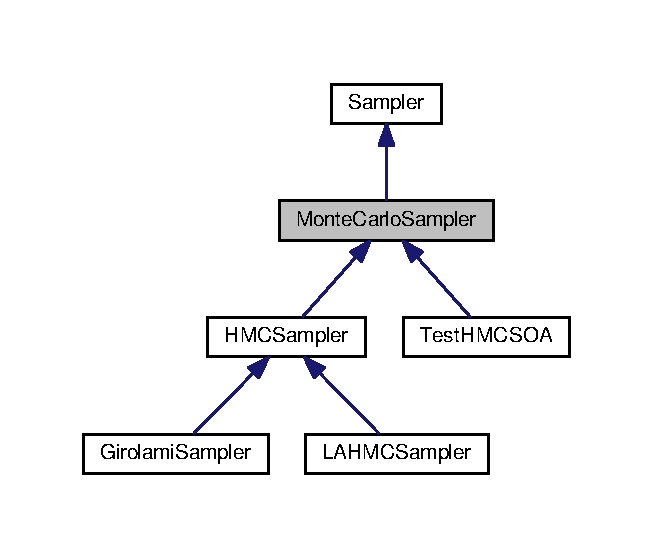
\includegraphics[width=314pt]{classMonteCarloSampler__inherit__graph}
\end{center}
\end{figure}


Collaboration diagram for Monte\+Carlo\+Sampler\+:\nopagebreak
\begin{figure}[H]
\begin{center}
\leavevmode
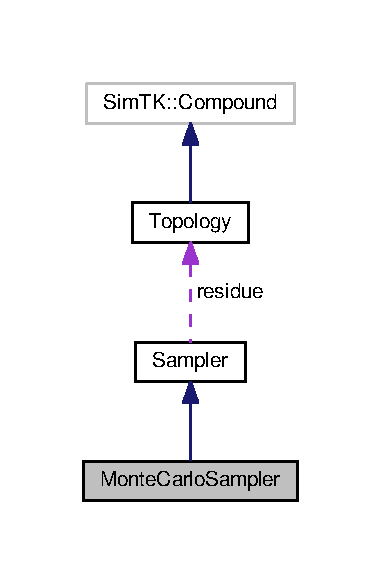
\includegraphics[width=183pt]{classMonteCarloSampler__coll__graph}
\end{center}
\end{figure}
\subsection*{Public Member Functions}
\begin{DoxyCompactItemize}
\item 
{\bfseries Monte\+Carlo\+Sampler} (Sim\+T\+K\+::\+Compound\+System $\ast$arg\+Compound\+System, Sim\+T\+K\+::\+Simbody\+Matter\+Subsystem $\ast$arg\+Matter, std\+::vector$<$ \hyperlink{classTopology}{Topology} $\ast$ $>$ \&arg\+Topologies, Sim\+T\+K\+::\+Du\+M\+M\+Force\+Field\+Subsystem $\ast$arg\+Dumm, Sim\+T\+K\+::\+General\+Force\+Subsystem $\ast$forces, Sim\+T\+K\+::\+Time\+Stepper $\ast$arg\+Time\+Stepper)\hypertarget{classMonteCarloSampler_a07b24155322212a06eaee8e945e349ee}{}\label{classMonteCarloSampler_a07b24155322212a06eaee8e945e349ee}

\item 
void {\bfseries set\+Thermostat} (Thermostat\+Name)\hypertarget{classMonteCarloSampler_a1ead7846108a3fc20f01c97442c39c17}{}\label{classMonteCarloSampler_a1ead7846108a3fc20f01c97442c39c17}

\item 
void {\bfseries set\+Thermostat} (std\+::string)\hypertarget{classMonteCarloSampler_aefbf81422671bbf30387e1d710f81147}{}\label{classMonteCarloSampler_aefbf81422671bbf30387e1d710f81147}

\item 
void {\bfseries set\+Thermostat} (const char $\ast$)\hypertarget{classMonteCarloSampler_a405e4793d80178a19cd46664ba3b2ad2}{}\label{classMonteCarloSampler_a405e4793d80178a19cd46664ba3b2ad2}

\item 
virtual Thermostat\+Name {\bfseries get\+Thermostat} (void) const \hypertarget{classMonteCarloSampler_a058662609fcf2d35bb4c1d68754c73e1}{}\label{classMonteCarloSampler_a058662609fcf2d35bb4c1d68754c73e1}

\item 
virtual void \hyperlink{classMonteCarloSampler_a1063f1111e793d942f35481a4d7346d7}{initialize} (Sim\+T\+K\+::\+State \&advanced, Sim\+T\+K\+::\+Real arg\+Temperature, bool arg\+Use\+Fixman=true)
\item 
virtual void \hyperlink{classMonteCarloSampler_a4e085e821dffa919cc385a2b052603cc}{reinitialize} (Sim\+T\+K\+::\+State \&advanced, Sim\+T\+K\+::\+Real arg\+Temperature)
\item 
void {\bfseries set\+Set\+T\+Vector} (const Sim\+T\+K\+::\+State \&advanced)\hypertarget{classMonteCarloSampler_a49ddb4d4f1d48b9fd3d6f9b1bc9762be}{}\label{classMonteCarloSampler_a49ddb4d4f1d48b9fd3d6f9b1bc9762be}

\item 
Sim\+T\+K\+::\+Transform $\ast$ {\bfseries get\+Set\+T\+Vector} (void)\hypertarget{classMonteCarloSampler_a381114ca6245e61809691a5b8efec354}{}\label{classMonteCarloSampler_a381114ca6245e61809691a5b8efec354}

\item 
void {\bfseries assign\+Conf\+From\+Set\+T\+Vector} (Sim\+T\+K\+::\+State \&advanced)\hypertarget{classMonteCarloSampler_aff4c58f725a9b1b5cafe1e6afe70272a}{}\label{classMonteCarloSampler_aff4c58f725a9b1b5cafe1e6afe70272a}

\item 
void {\bfseries set\+T\+Vector} (const Sim\+T\+K\+::\+State \&advanced)\hypertarget{classMonteCarloSampler_af8cbc49beae7f81cc0d560953424b049}{}\label{classMonteCarloSampler_af8cbc49beae7f81cc0d560953424b049}

\item 
void {\bfseries set\+T\+Vector} (Sim\+T\+K\+::\+Transform $\ast$)\hypertarget{classMonteCarloSampler_a42c51f9eb62489ebb715a945742556b2}{}\label{classMonteCarloSampler_a42c51f9eb62489ebb715a945742556b2}

\item 
Sim\+T\+K\+::\+Transform $\ast$ {\bfseries get\+T\+Vector} (void)\hypertarget{classMonteCarloSampler_a010b453ab1e2cf910370c2a983ac9459}{}\label{classMonteCarloSampler_a010b453ab1e2cf910370c2a983ac9459}

\item 
void {\bfseries assign\+Conf\+From\+T\+Vector} (Sim\+T\+K\+::\+State \&advanced)\hypertarget{classMonteCarloSampler_ab72a7be6ee6960ed6695276d1ae7f81e}{}\label{classMonteCarloSampler_ab72a7be6ee6960ed6695276d1ae7f81e}

\item 
void \hyperlink{classMonteCarloSampler_af35ad7b12d462b867b968e3ec8194c05}{propose} (Sim\+T\+K\+::\+State \&advanced)
\item 
void {\bfseries update} (Sim\+T\+K\+::\+State \&)\hypertarget{classMonteCarloSampler_aea26d5e94570b2c3ba27e4b8c75de3ac}{}\label{classMonteCarloSampler_aea26d5e94570b2c3ba27e4b8c75de3ac}

\item 
Sim\+T\+K\+::\+Real {\bfseries get\+Set\+PE} (void) const \hypertarget{classMonteCarloSampler_a574c8cc51d4d4a77dff0094a8bf7ab94}{}\label{classMonteCarloSampler_a574c8cc51d4d4a77dff0094a8bf7ab94}

\item 
void {\bfseries set\+Set\+PE} (Sim\+T\+K\+::\+Real arg\+PE)\hypertarget{classMonteCarloSampler_aee20844deef1624d0e49133b5da7267d}{}\label{classMonteCarloSampler_aee20844deef1624d0e49133b5da7267d}

\item 
Sim\+T\+K\+::\+Real {\bfseries get\+Old\+PE} (void) const \hypertarget{classMonteCarloSampler_ad1248e740d46b90e0f2cfcdeaa94fc92}{}\label{classMonteCarloSampler_ad1248e740d46b90e0f2cfcdeaa94fc92}

\item 
void {\bfseries set\+Old\+PE} (Sim\+T\+K\+::\+Real arg\+PE)\hypertarget{classMonteCarloSampler_a541f5de0ef4ee9ec8963d11750be4b9b}{}\label{classMonteCarloSampler_a541f5de0ef4ee9ec8963d11750be4b9b}

\item 
void {\bfseries set\+Set\+Fixman} (Sim\+T\+K\+::\+Real)\hypertarget{classMonteCarloSampler_a5bc8474546ba1a04a7dc9c37069963b2}{}\label{classMonteCarloSampler_a5bc8474546ba1a04a7dc9c37069963b2}

\item 
Sim\+T\+K\+::\+Real {\bfseries get\+Set\+Fixman} (void) const \hypertarget{classMonteCarloSampler_ad0f7f3e1554620e467e1f519a7600736}{}\label{classMonteCarloSampler_ad0f7f3e1554620e467e1f519a7600736}

\item 
void {\bfseries set\+R\+EP} (Sim\+T\+K\+::\+Real)\hypertarget{classMonteCarloSampler_a8dc6b458ce92bb91396e92d172fc94fc}{}\label{classMonteCarloSampler_a8dc6b458ce92bb91396e92d172fc94fc}

\item 
Sim\+T\+K\+::\+Real {\bfseries get\+R\+EP} (void) const \hypertarget{classMonteCarloSampler_a9b525f238f6290d2b74680ca96425db7}{}\label{classMonteCarloSampler_a9b525f238f6290d2b74680ca96425db7}

\item 
void {\bfseries set\+Old\+Fixman} (Sim\+T\+K\+::\+Real)\hypertarget{classMonteCarloSampler_a45c88aa68467e55b253f4d38aa044663}{}\label{classMonteCarloSampler_a45c88aa68467e55b253f4d38aa044663}

\item 
Sim\+T\+K\+::\+Real {\bfseries get\+Old\+Fixman} (void) const \hypertarget{classMonteCarloSampler_a14aa5d89fd3832ebb63b2cff48d76fd2}{}\label{classMonteCarloSampler_a14aa5d89fd3832ebb63b2cff48d76fd2}

\item 
void {\bfseries set\+Set\+Log\+Sine\+Sqr\+Gamma2} (Sim\+T\+K\+::\+Real)\hypertarget{classMonteCarloSampler_a569d624b7c74ebffecb31153231c7314}{}\label{classMonteCarloSampler_a569d624b7c74ebffecb31153231c7314}

\item 
Sim\+T\+K\+::\+Real {\bfseries get\+Set\+Log\+Sine\+Sqr\+Gamma2} (void) const \hypertarget{classMonteCarloSampler_a091f14ccd03de6141b247a4f0c4775b7}{}\label{classMonteCarloSampler_a091f14ccd03de6141b247a4f0c4775b7}

\item 
void {\bfseries set\+Old\+Log\+Sine\+Sqr\+Gamma2} (Sim\+T\+K\+::\+Real)\hypertarget{classMonteCarloSampler_a78930927d4a5b5d201f38cdd5e438f88}{}\label{classMonteCarloSampler_a78930927d4a5b5d201f38cdd5e438f88}

\item 
Sim\+T\+K\+::\+Real {\bfseries get\+Old\+Log\+Sine\+Sqr\+Gamma2} (void) const \hypertarget{classMonteCarloSampler_a3120cbf9c30baff5a64f02f38767472b}{}\label{classMonteCarloSampler_a3120cbf9c30baff5a64f02f38767472b}

\item 
void {\bfseries set\+Proposed\+Log\+Sine\+Sqr\+Gamma2} (Sim\+T\+K\+::\+Real arg\+Fixman)\hypertarget{classMonteCarloSampler_aee0045dca052c0a485c36175a1818e77}{}\label{classMonteCarloSampler_aee0045dca052c0a485c36175a1818e77}

\item 
Sim\+T\+K\+::\+Real {\bfseries get\+Proposed\+Log\+Sine\+Sqr\+Gamma2} (void) const \hypertarget{classMonteCarloSampler_af3dc14be70f4a1fc565e557633932db1}{}\label{classMonteCarloSampler_af3dc14be70f4a1fc565e557633932db1}

\item 
void {\bfseries set\+Proposed\+Fixman} (Sim\+T\+K\+::\+Real)\hypertarget{classMonteCarloSampler_a8b36193b2d296fc2f3b3dd2c56e41aa9}{}\label{classMonteCarloSampler_a8b36193b2d296fc2f3b3dd2c56e41aa9}

\item 
Sim\+T\+K\+::\+Real {\bfseries get\+Proposed\+Fixman} (void) const \hypertarget{classMonteCarloSampler_aa2e8b879e996bd6f9b226657d3ed3a63}{}\label{classMonteCarloSampler_aa2e8b879e996bd6f9b226657d3ed3a63}

\item 
Sim\+T\+K\+::\+Real {\bfseries get\+P\+E\+From\+Evaluator} (Sim\+T\+K\+::\+State \&some\+State)\hypertarget{classMonteCarloSampler_af535395968c8aedfcb98836f61a0594f}{}\label{classMonteCarloSampler_af535395968c8aedfcb98836f61a0594f}

\item 
void {\bfseries use\+Fixman\+Potential} (void)\hypertarget{classMonteCarloSampler_a8f47fe7010dd8c087e386af08e6b17bf}{}\label{classMonteCarloSampler_a8f47fe7010dd8c087e386af08e6b17bf}

\item 
bool {\bfseries is\+Using\+Fixman\+Potential} (void) const \hypertarget{classMonteCarloSampler_a16b691acfbbb0489b79949053610adea}{}\label{classMonteCarloSampler_a16b691acfbbb0489b79949053610adea}

\item 
Sim\+T\+K\+::\+Real {\bfseries calc\+Fixman} (Sim\+T\+K\+::\+State \&some\+State)\hypertarget{classMonteCarloSampler_a7865bdccd1f6d03efa08978b2fd943fe}{}\label{classMonteCarloSampler_a7865bdccd1f6d03efa08978b2fd943fe}

\item 
Sim\+T\+K\+::\+Real {\bfseries calc\+Num\+Fixman} (Sim\+T\+K\+::\+State \&some\+State)\hypertarget{classMonteCarloSampler_a9b94172a710aebf05d4ddbb889991f46}{}\label{classMonteCarloSampler_a9b94172a710aebf05d4ddbb889991f46}

\item 
Sim\+T\+K\+::\+Real {\bfseries calc\+Num\+DetM} (Sim\+T\+K\+::\+State \&some\+State)\hypertarget{classMonteCarloSampler_acf6a189a1c0d4c19b51d768341a4efe0}{}\label{classMonteCarloSampler_acf6a189a1c0d4c19b51d768341a4efe0}

\item 
void {\bfseries send\+Conf\+To\+Evaluator} (void)\hypertarget{classMonteCarloSampler_ad82ab3bef1e3fd97c6abf697738792a6}{}\label{classMonteCarloSampler_ad82ab3bef1e3fd97c6abf697738792a6}

\item 
bool {\bfseries get\+Always\+Accept} (void) const \hypertarget{classMonteCarloSampler_a6eab6650da5aab47299128f806228e8f}{}\label{classMonteCarloSampler_a6eab6650da5aab47299128f806228e8f}

\item 
void {\bfseries set\+Always\+Accept} (bool)\hypertarget{classMonteCarloSampler_a93d9574f30822b76ca34ee916c4eb5fa}{}\label{classMonteCarloSampler_a93d9574f30822b76ca34ee916c4eb5fa}

\item 
int {\bfseries get\+Accepted\+Steps} (void) const \hypertarget{classMonteCarloSampler_a2bb387a9068adf5861c7ca63b2c65641}{}\label{classMonteCarloSampler_a2bb387a9068adf5861c7ca63b2c65641}

\end{DoxyCompactItemize}
\subsection*{Protected Attributes}
\begin{DoxyCompactItemize}
\item 
std\+::vector$<$ Sim\+T\+K\+::\+Transform $>$ {\bfseries Set\+T\+Vector}\hypertarget{classMonteCarloSampler_a4c863be2e5ebefe4e923caf007c7fde9}{}\label{classMonteCarloSampler_a4c863be2e5ebefe4e923caf007c7fde9}

\item 
std\+::vector$<$ Sim\+T\+K\+::\+Transform $>$ {\bfseries T\+Vector}\hypertarget{classMonteCarloSampler_af5fea1471133f61f5f5f05ab302f4562}{}\label{classMonteCarloSampler_af5fea1471133f61f5f5f05ab302f4562}

\item 
Sim\+T\+K\+::\+Real {\bfseries pe\+\_\+set} = 0.\+0\hypertarget{classMonteCarloSampler_a08775705779aed062ed86216b538f03b}{}\label{classMonteCarloSampler_a08775705779aed062ed86216b538f03b}

\item 
Sim\+T\+K\+::\+Real {\bfseries pe\+\_\+o} = 0.\+0\hypertarget{classMonteCarloSampler_a07f4e95e16aa27c6fd424d900c45e94d}{}\label{classMonteCarloSampler_a07f4e95e16aa27c6fd424d900c45e94d}

\item 
Sim\+T\+K\+::\+Real {\bfseries pe\+\_\+n} = 0.\+0\hypertarget{classMonteCarloSampler_a7c5b417b17d79468129b03fe5398c482}{}\label{classMonteCarloSampler_a7c5b417b17d79468129b03fe5398c482}

\item 
Sim\+T\+K\+::\+Real {\bfseries fix\+\_\+set} = 0.\+0\hypertarget{classMonteCarloSampler_a9f27d9e958e6911fa3b8fb13cb1d2481}{}\label{classMonteCarloSampler_a9f27d9e958e6911fa3b8fb13cb1d2481}

\item 
Sim\+T\+K\+::\+Real {\bfseries fix\+\_\+o} = 0.\+0\hypertarget{classMonteCarloSampler_ae6919d5694b0417b337f768d3a62aded}{}\label{classMonteCarloSampler_ae6919d5694b0417b337f768d3a62aded}

\item 
Sim\+T\+K\+::\+Real {\bfseries fix\+\_\+n} = 0.\+0\hypertarget{classMonteCarloSampler_a672a0893caefef6136ed20e125f47275}{}\label{classMonteCarloSampler_a672a0893caefef6136ed20e125f47275}

\item 
Sim\+T\+K\+::\+Real {\bfseries detmbat\+\_\+set} = 0.\+0\hypertarget{classMonteCarloSampler_a258169bc588eb202b488a7a7941c446e}{}\label{classMonteCarloSampler_a258169bc588eb202b488a7a7941c446e}

\item 
Sim\+T\+K\+::\+Real {\bfseries detmbat\+\_\+o} = 0.\+0\hypertarget{classMonteCarloSampler_aa6ab3bf81da9dd54c0df1afbb92c94d5}{}\label{classMonteCarloSampler_aa6ab3bf81da9dd54c0df1afbb92c94d5}

\item 
Sim\+T\+K\+::\+Real {\bfseries detmbat\+\_\+n} = 0.\+0\hypertarget{classMonteCarloSampler_a1c11d5fd863c257f32ab142b7e65648b}{}\label{classMonteCarloSampler_a1c11d5fd863c257f32ab142b7e65648b}

\item 
Sim\+T\+K\+::\+Real {\bfseries residual\+Embedded\+Potential} = 0.\+0\hypertarget{classMonteCarloSampler_a1c6167653e0d2fa65057a6a4793faea1}{}\label{classMonteCarloSampler_a1c6167653e0d2fa65057a6a4793faea1}

\item 
Sim\+T\+K\+::\+Real {\bfseries log\+Sine\+Sqr\+Gamma2\+\_\+o} = 0.\+0\hypertarget{classMonteCarloSampler_a451404c5869285d32047cd8070f31dc3}{}\label{classMonteCarloSampler_a451404c5869285d32047cd8070f31dc3}

\item 
Sim\+T\+K\+::\+Real {\bfseries log\+Sine\+Sqr\+Gamma2\+\_\+n} = 0.\+0\hypertarget{classMonteCarloSampler_aad0a503a222d06dafd504bbd6c4c2d4a}{}\label{classMonteCarloSampler_aad0a503a222d06dafd504bbd6c4c2d4a}

\item 
Sim\+T\+K\+::\+Real {\bfseries log\+Sine\+Sqr\+Gamma2\+\_\+set} = 0.\+0\hypertarget{classMonteCarloSampler_a2c9848636e1842bbeb0a5e86dd039007}{}\label{classMonteCarloSampler_a2c9848636e1842bbeb0a5e86dd039007}

\item 
bool {\bfseries use\+Fixman} = false\hypertarget{classMonteCarloSampler_a202a86fee8c6c766d68d4a6d44918ebf}{}\label{classMonteCarloSampler_a202a86fee8c6c766d68d4a6d44918ebf}

\item 
bool {\bfseries always\+Accept} = false\hypertarget{classMonteCarloSampler_a1deab6aec5c368a516afced6dc87b001}{}\label{classMonteCarloSampler_a1deab6aec5c368a516afced6dc87b001}

\item 
int {\bfseries accepted\+Steps} = 0\hypertarget{classMonteCarloSampler_ac2b9df435ba70cedd43406dc66d691b7}{}\label{classMonteCarloSampler_ac2b9df435ba70cedd43406dc66d691b7}

\item 
int {\bfseries accepted\+Steps\+Buffer\+Size} = 30\hypertarget{classMonteCarloSampler_a25ebd711aad3d3be594978679a292805}{}\label{classMonteCarloSampler_a25ebd711aad3d3be594978679a292805}

\item 
std\+::list$<$ int $>$ {\bfseries accepted\+Steps\+Buffer}\hypertarget{classMonteCarloSampler_adf63689df579ac22e76d47380a0b6341}{}\label{classMonteCarloSampler_adf63689df579ac22e76d47380a0b6341}

\item 
int {\bfseries Qs\+Buffer\+Size} = 300\hypertarget{classMonteCarloSampler_a0720d9d5e4543b23006a5c7616269756}{}\label{classMonteCarloSampler_a0720d9d5e4543b23006a5c7616269756}

\item 
std\+::list$<$ Sim\+T\+K\+::\+Real $>$ {\bfseries Qs\+Buffer}\hypertarget{classMonteCarloSampler_aa1f3656e46752f5fe9f4868d2658d18a}{}\label{classMonteCarloSampler_aa1f3656e46752f5fe9f4868d2658d18a}

\item 
float {\bfseries acceptance}\hypertarget{classMonteCarloSampler_a1006f1adddf4666a094e6eb19c3065b7}{}\label{classMonteCarloSampler_a1006f1adddf4666a094e6eb19c3065b7}

\item 
float {\bfseries prev\+Acceptance}\hypertarget{classMonteCarloSampler_a8b725ad99341adf348645390311089e7}{}\label{classMonteCarloSampler_a8b725ad99341adf348645390311089e7}

\item 
float {\bfseries prev\+Prev\+Acceptance}\hypertarget{classMonteCarloSampler_ae59ce9e6f6d0fd91da053fecdba7b7ba}{}\label{classMonteCarloSampler_ae59ce9e6f6d0fd91da053fecdba7b7ba}

\item 
bool {\bfseries propose\+Exception\+Caught}\hypertarget{classMonteCarloSampler_af6b5f8a5682111329963b546b3f3de65}{}\label{classMonteCarloSampler_af6b5f8a5682111329963b546b3f3de65}

\end{DoxyCompactItemize}
\subsection*{Friends}
\begin{DoxyCompactItemize}
\item 
class {\bfseries Context}\hypertarget{classMonteCarloSampler_ac26c806e60ca4a0547680edb68f6e39b}{}\label{classMonteCarloSampler_ac26c806e60ca4a0547680edb68f6e39b}

\end{DoxyCompactItemize}
\subsection*{Additional Inherited Members}


\subsection{Member Function Documentation}
\index{Monte\+Carlo\+Sampler@{Monte\+Carlo\+Sampler}!initialize@{initialize}}
\index{initialize@{initialize}!Monte\+Carlo\+Sampler@{Monte\+Carlo\+Sampler}}
\subsubsection[{\texorpdfstring{initialize(\+Sim\+T\+K\+::\+State \&advanced, Sim\+T\+K\+::\+Real arg\+Temperature, bool arg\+Use\+Fixman=true)}{initialize(SimTK::State &advanced, SimTK::Real argTemperature, bool argUseFixman=true)}}]{\setlength{\rightskip}{0pt plus 5cm}void Monte\+Carlo\+Sampler\+::initialize (
\begin{DoxyParamCaption}
\item[{Sim\+T\+K\+::\+State \&}]{advanced, }
\item[{Sim\+T\+K\+::\+Real}]{arg\+Temperature, }
\item[{bool}]{arg\+Use\+Fixman = {\ttfamily true}}
\end{DoxyParamCaption}
)\hspace{0.3cm}{\ttfamily [virtual]}}\hypertarget{classMonteCarloSampler_a1063f1111e793d942f35481a4d7346d7}{}\label{classMonteCarloSampler_a1063f1111e793d942f35481a4d7346d7}
Seed the random number generator. Set simulation temperature, variables that store the configuration and variables that store the energies, both needed for the acception-\/rejection step. Also realize velocities and initialize the timestepper. \index{Monte\+Carlo\+Sampler@{Monte\+Carlo\+Sampler}!propose@{propose}}
\index{propose@{propose}!Monte\+Carlo\+Sampler@{Monte\+Carlo\+Sampler}}
\subsubsection[{\texorpdfstring{propose(\+Sim\+T\+K\+::\+State \&advanced)}{propose(SimTK::State &advanced)}}]{\setlength{\rightskip}{0pt plus 5cm}void Monte\+Carlo\+Sampler\+::propose (
\begin{DoxyParamCaption}
\item[{Sim\+T\+K\+::\+State \&}]{some\+State}
\end{DoxyParamCaption}
)\hspace{0.3cm}{\ttfamily [virtual]}}\hypertarget{classMonteCarloSampler_af35ad7b12d462b867b968e3ec8194c05}{}\label{classMonteCarloSampler_af35ad7b12d462b867b968e3ec8194c05}
Propose a move 

Implements \hyperlink{classSampler_a3022d2efacf6107b3fba506d31e2919e}{Sampler}.

\index{Monte\+Carlo\+Sampler@{Monte\+Carlo\+Sampler}!reinitialize@{reinitialize}}
\index{reinitialize@{reinitialize}!Monte\+Carlo\+Sampler@{Monte\+Carlo\+Sampler}}
\subsubsection[{\texorpdfstring{reinitialize(\+Sim\+T\+K\+::\+State \&advanced, Sim\+T\+K\+::\+Real arg\+Temperature)}{reinitialize(SimTK::State &advanced, SimTK::Real argTemperature)}}]{\setlength{\rightskip}{0pt plus 5cm}void Monte\+Carlo\+Sampler\+::reinitialize (
\begin{DoxyParamCaption}
\item[{Sim\+T\+K\+::\+State \&}]{advanced, }
\item[{Sim\+T\+K\+::\+Real}]{arg\+Temperature}
\end{DoxyParamCaption}
)\hspace{0.3cm}{\ttfamily [virtual]}}\hypertarget{classMonteCarloSampler_a4e085e821dffa919cc385a2b052603cc}{}\label{classMonteCarloSampler_a4e085e821dffa919cc385a2b052603cc}
Same as initialize 

The documentation for this class was generated from the following files\+:\begin{DoxyCompactItemize}
\item 
include/gmolmodel/Monte\+Carlo\+Sampler.\+hpp\item 
src/\hyperlink{MonteCarloSampler_8cpp}{Monte\+Carlo\+Sampler.\+cpp}\end{DoxyCompactItemize}

\hypertarget{classMyState}{}\section{My\+State Class Reference}
\label{classMyState}\index{My\+State@{My\+State}}


Inheritance diagram for My\+State\+:\nopagebreak
\begin{figure}[H]
\begin{center}
\leavevmode
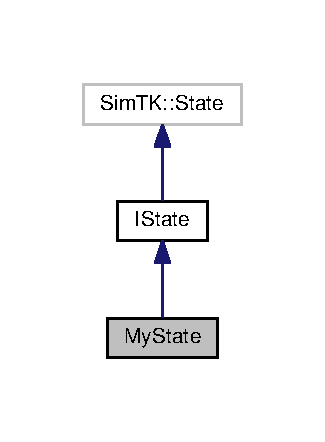
\includegraphics[width=156pt]{classMyState__inherit__graph}
\end{center}
\end{figure}


Collaboration diagram for My\+State\+:\nopagebreak
\begin{figure}[H]
\begin{center}
\leavevmode
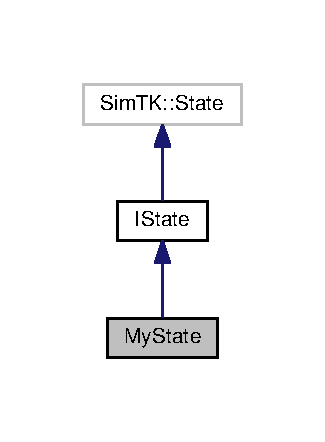
\includegraphics[width=156pt]{classMyState__coll__graph}
\end{center}
\end{figure}
\subsection*{Public Member Functions}
\begin{DoxyCompactItemize}
\item 
Sim\+T\+K\+::\+Vec3 {\bfseries get\+Cartesian} (int atom\+\_\+no)\hypertarget{classMyState_a769460770d243aa7f6e502e03a382176}{}\label{classMyState_a769460770d243aa7f6e502e03a382176}

\item 
void {\bfseries upd\+Cartesian} (int atom\+\_\+no, Sim\+T\+K\+::\+Real x, Sim\+T\+K\+::\+Real y, Sim\+T\+K\+::\+Real z)\hypertarget{classMyState_aea93f1c028d9b3b41d5a946b2bac6810}{}\label{classMyState_aea93f1c028d9b3b41d5a946b2bac6810}

\item 
void {\bfseries set\+Cartesian} (int atom\+\_\+no, Sim\+T\+K\+::\+Real x, Sim\+T\+K\+::\+Real y, Sim\+T\+K\+::\+Real z)\hypertarget{classMyState_a0b4fe1fc80f10af1430abc298c369f77}{}\label{classMyState_a0b4fe1fc80f10af1430abc298c369f77}

\end{DoxyCompactItemize}


The documentation for this class was generated from the following files\+:\begin{DoxyCompactItemize}
\item 
include/gmolmodel/My\+State.\+hpp\item 
src/My\+State.\+cpp\end{DoxyCompactItemize}

\hypertarget{classNonbondedForceTask}{}\section{Nonbonded\+Force\+Task Class Reference}
\label{classNonbondedForceTask}\index{Nonbonded\+Force\+Task@{Nonbonded\+Force\+Task}}


Inheritance diagram for Nonbonded\+Force\+Task\+:
\nopagebreak
\begin{figure}[H]
\begin{center}
\leavevmode
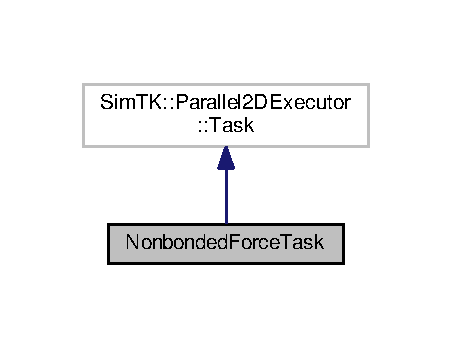
\includegraphics[width=217pt]{classNonbondedForceTask__inherit__graph}
\end{center}
\end{figure}


Collaboration diagram for Nonbonded\+Force\+Task\+:
\nopagebreak
\begin{figure}[H]
\begin{center}
\leavevmode
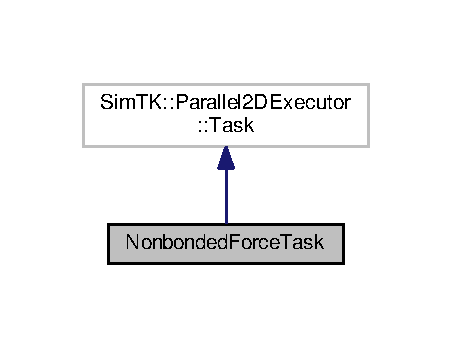
\includegraphics[width=217pt]{classNonbondedForceTask__coll__graph}
\end{center}
\end{figure}
\subsection*{Public Member Functions}
\begin{DoxyCompactItemize}
\item 
{\bfseries Nonbonded\+Force\+Task} (int mat4x4\mbox{[}4\mbox{]}\mbox{[}4\mbox{]}, int \&\+\_\+total)\hypertarget{classNonbondedForceTask_a343846e6c771df61e839f308e871e106}{}\label{classNonbondedForceTask_a343846e6c771df61e839f308e871e106}

\item 
void {\bfseries initialize} ()\hypertarget{classNonbondedForceTask_a8e0d4a4ed119acdcf0321f838f21e352}{}\label{classNonbondedForceTask_a8e0d4a4ed119acdcf0321f838f21e352}

\item 
void {\bfseries finish} ()\hypertarget{classNonbondedForceTask_a3efba9c05eec3d517a2f74510f24a596}{}\label{classNonbondedForceTask_a3efba9c05eec3d517a2f74510f24a596}

\item 
void {\bfseries execute} (int body1, int body2)\hypertarget{classNonbondedForceTask_a58d621a99f49bddad3405fe15d4e6cc1}{}\label{classNonbondedForceTask_a58d621a99f49bddad3405fe15d4e6cc1}

\end{DoxyCompactItemize}


The documentation for this class was generated from the following file\+:\begin{DoxyCompactItemize}
\item 
tests/Test\+Parallel\+Executor.\+cpp\end{DoxyCompactItemize}

\hypertarget{classParaMolecularDecorator}{}\section{Para\+Molecular\+Decorator Class Reference}
\label{classParaMolecularDecorator}\index{Para\+Molecular\+Decorator@{Para\+Molecular\+Decorator}}


Inheritance diagram for Para\+Molecular\+Decorator\+:\nopagebreak
\begin{figure}[H]
\begin{center}
\leavevmode
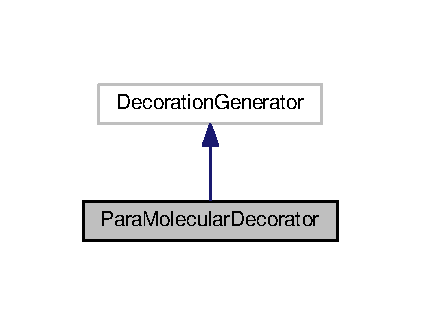
\includegraphics[width=202pt]{classParaMolecularDecorator__inherit__graph}
\end{center}
\end{figure}


Collaboration diagram for Para\+Molecular\+Decorator\+:\nopagebreak
\begin{figure}[H]
\begin{center}
\leavevmode
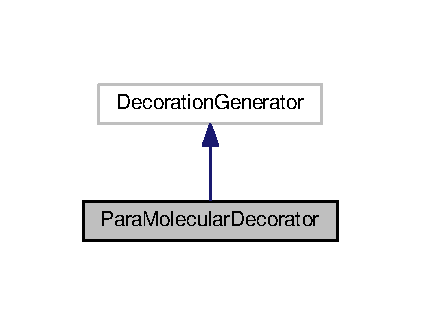
\includegraphics[width=202pt]{classParaMolecularDecorator__coll__graph}
\end{center}
\end{figure}
\subsection*{Public Member Functions}
\begin{DoxyCompactItemize}
\item 
{\bfseries Para\+Molecular\+Decorator} (Sim\+T\+K\+::\+Compound\+System $\ast$arg\+Compound\+System, Sim\+T\+K\+::\+Simbody\+Matter\+Subsystem $\ast$arg\+Matter, Sim\+T\+K\+::\+Du\+M\+M\+Force\+Field\+Subsystem $\ast$arg\+Dumm, Sim\+T\+K\+::\+General\+Force\+Subsystem $\ast$arg\+Forces)\hypertarget{classParaMolecularDecorator_a00ee22ac14c9bd33771b4006bcae55e5}{}\label{classParaMolecularDecorator_a00ee22ac14c9bd33771b4006bcae55e5}

\item 
void {\bfseries Add\+Molecule} (\hyperlink{classTopology}{Topology} $\ast$arg\+Molecule)\hypertarget{classParaMolecularDecorator_a23ac037154120e14574aeed3e5a300b6}{}\label{classParaMolecularDecorator_a23ac037154120e14574aeed3e5a300b6}

\item 
void {\bfseries load\+Point} (const Vec3 point)\hypertarget{classParaMolecularDecorator_aef3764d8a79b7a888be38db7c4715529}{}\label{classParaMolecularDecorator_aef3764d8a79b7a888be38db7c4715529}

\item 
void {\bfseries load\+Line} (const Vec3 p1, const Vec3 p2)\hypertarget{classParaMolecularDecorator_a13cdd8929af06e78706d43a80cdde877}{}\label{classParaMolecularDecorator_a13cdd8929af06e78706d43a80cdde877}

\item 
void {\bfseries clear\+Points} (void)\hypertarget{classParaMolecularDecorator_a75516eeec18b6629281fffe64c6e33e2}{}\label{classParaMolecularDecorator_a75516eeec18b6629281fffe64c6e33e2}

\item 
void {\bfseries clear\+Lines} (void)\hypertarget{classParaMolecularDecorator_aeca0898301083dfdb525e3d65306de65}{}\label{classParaMolecularDecorator_aeca0898301083dfdb525e3d65306de65}

\item 
void \hyperlink{classParaMolecularDecorator_a9d92eb6838610d91b6933dffd415e061}{generate\+Decorations} (const State \&state, Array\+\_\+$<$ Decorative\+Geometry $>$ \&geometry)
\item 
void {\bfseries set\+Atom\+Targets} (std\+::vector$<$ std\+::pair$<$ \hyperlink{classbSpecificAtom}{b\+Specific\+Atom} $\ast$, Sim\+T\+K\+::\+Vec3 $>$$>$ residue\+Atom\+Locations)\hypertarget{classParaMolecularDecorator_a8d4f8fd75c3e98b2f94778d1139e302a}{}\label{classParaMolecularDecorator_a8d4f8fd75c3e98b2f94778d1139e302a}

\end{DoxyCompactItemize}


\subsection{Member Function Documentation}
\index{Para\+Molecular\+Decorator@{Para\+Molecular\+Decorator}!generate\+Decorations@{generate\+Decorations}}
\index{generate\+Decorations@{generate\+Decorations}!Para\+Molecular\+Decorator@{Para\+Molecular\+Decorator}}
\subsubsection[{\texorpdfstring{generate\+Decorations(const State \&state, Array\+\_\+$<$ Decorative\+Geometry $>$ \&geometry)}{generateDecorations(const State &state, Array_< DecorativeGeometry > &geometry)}}]{\setlength{\rightskip}{0pt plus 5cm}void Para\+Molecular\+Decorator\+::generate\+Decorations (
\begin{DoxyParamCaption}
\item[{const State \&}]{state, }
\item[{Array\+\_\+$<$ Decorative\+Geometry $>$ \&}]{geometry}
\end{DoxyParamCaption}
)}\hypertarget{classParaMolecularDecorator_a9d92eb6838610d91b6933dffd415e061}{}\label{classParaMolecularDecorator_a9d92eb6838610d91b6933dffd415e061}

\begin{DoxyItemize}
\item 
\item 
\end{DoxyItemize}

The documentation for this class was generated from the following files\+:\begin{DoxyCompactItemize}
\item 
include/gmolmodel/Para\+Molecular\+Decorator.\+hpp\item 
src/\hyperlink{ParaMolecularDecorator_8cpp}{Para\+Molecular\+Decorator.\+cpp}\end{DoxyCompactItemize}

\hypertarget{classPDBObject}{}\section{P\+D\+B\+Object Class Reference}
\label{classPDBObject}\index{P\+D\+B\+Object@{P\+D\+B\+Object}}
\subsection*{Public Member Functions}
\begin{DoxyCompactItemize}
\item 
void {\bfseries read\+P\+D\+Bfile} (std\+::string pdbfile)\hypertarget{classPDBObject_acdac2e8167f94f020e53f7eb96ce21ca}{}\label{classPDBObject_acdac2e8167f94f020e53f7eb96ce21ca}

\item 
void {\bfseries write\+P\+D\+Bfile} (std\+::string pdbfile, std\+::vector$<$ std\+::string $>$ Atoms\+Name, std\+::vector$<$ std\+::string $>$ Atoms\+Mol\+Name, std\+::vector$<$ std\+::string $>$ Atoms\+Chain, std\+::vector$<$ int $>$ Atoms\+Mol\+No, std\+::vector$<$ T\+A\+R\+G\+E\+T\+\_\+\+T\+Y\+PE $>$ Atoms\+Xcoord, std\+::vector$<$ T\+A\+R\+G\+E\+T\+\_\+\+T\+Y\+PE $>$ Atoms\+Ycoord, std\+::vector$<$ T\+A\+R\+G\+E\+T\+\_\+\+T\+Y\+PE $>$ Atoms\+Zcoord, std\+::vector$<$ std\+::string $>$ Atoms1\+Character)\hypertarget{classPDBObject_a19e921655d782bf8614ecab54e408789}{}\label{classPDBObject_a19e921655d782bf8614ecab54e408789}

\item 
int {\bfseries get\+Number\+Atoms} ()\hypertarget{classPDBObject_a3fa44a49172e37fe4dc7f4a7f6efa04c}{}\label{classPDBObject_a3fa44a49172e37fe4dc7f4a7f6efa04c}

\item 
std\+::string {\bfseries get\+Atoms\+Name} (int p)\hypertarget{classPDBObject_a4a7ff5b9a86ae01570551c2d2cef34be}{}\label{classPDBObject_a4a7ff5b9a86ae01570551c2d2cef34be}

\item 
std\+::string {\bfseries get\+Atoms\+Mol\+Name} (int p)\hypertarget{classPDBObject_acbe90334ea558ca5b72ca3598614d0cf}{}\label{classPDBObject_acbe90334ea558ca5b72ca3598614d0cf}

\item 
std\+::string {\bfseries get\+Atoms\+Chain} (int p)\hypertarget{classPDBObject_a4ad2e68acbc220b6e721ad8ac99d236a}{}\label{classPDBObject_a4ad2e68acbc220b6e721ad8ac99d236a}

\item 
std\+::string {\bfseries get\+Atoms1\+Character} (int p)\hypertarget{classPDBObject_ab0073b4e0fa3c2b93aa6c73698b864ce}{}\label{classPDBObject_ab0073b4e0fa3c2b93aa6c73698b864ce}

\item 
int {\bfseries get\+Atoms\+Mol\+No} (int p)\hypertarget{classPDBObject_afac8cfcada83e8f8e15c21d5860ac3d9}{}\label{classPDBObject_afac8cfcada83e8f8e15c21d5860ac3d9}

\item 
T\+A\+R\+G\+E\+T\+\_\+\+T\+Y\+PE {\bfseries get\+Atoms\+Xcoord} (int p)\hypertarget{classPDBObject_a38b48008c620ceb4c9df543efd93501d}{}\label{classPDBObject_a38b48008c620ceb4c9df543efd93501d}

\item 
T\+A\+R\+G\+E\+T\+\_\+\+T\+Y\+PE {\bfseries get\+Atoms\+Ycoord} (int p)\hypertarget{classPDBObject_a502bd966236202509887461ab7a9583a}{}\label{classPDBObject_a502bd966236202509887461ab7a9583a}

\item 
T\+A\+R\+G\+E\+T\+\_\+\+T\+Y\+PE {\bfseries get\+Atoms\+Zcoord} (int p)\hypertarget{classPDBObject_a4f82cd26a531f894dce028dccab9199e}{}\label{classPDBObject_a4f82cd26a531f894dce028dccab9199e}

\end{DoxyCompactItemize}
\subsection*{Public Attributes}
\begin{DoxyCompactItemize}
\item 
std\+::ifstream {\bfseries pdbinput}\hypertarget{classPDBObject_ab08b53055c06295722ccf4fbc6285140}{}\label{classPDBObject_ab08b53055c06295722ccf4fbc6285140}

\item 
int {\bfseries Number\+Atoms}\hypertarget{classPDBObject_a4f3b486261366a7f54388a5ae49ddb29}{}\label{classPDBObject_a4f3b486261366a7f54388a5ae49ddb29}

\item 
std\+::vector$<$ std\+::string $>$ {\bfseries Atoms\+Name}\hypertarget{classPDBObject_af47560730130db2c9283bab146e5bc14}{}\label{classPDBObject_af47560730130db2c9283bab146e5bc14}

\item 
std\+::vector$<$ std\+::string $>$ {\bfseries Atoms\+Mol\+Name}\hypertarget{classPDBObject_ad5e1ed3a98c12156706b338068f675fb}{}\label{classPDBObject_ad5e1ed3a98c12156706b338068f675fb}

\item 
std\+::vector$<$ std\+::string $>$ {\bfseries Atoms\+Chain}\hypertarget{classPDBObject_a757696155e3ca58aefe5e2e2d38f987a}{}\label{classPDBObject_a757696155e3ca58aefe5e2e2d38f987a}

\item 
std\+::vector$<$ int $>$ {\bfseries Atoms\+Mol\+No}\hypertarget{classPDBObject_af623e48e95e436dfcb982dc080392a93}{}\label{classPDBObject_af623e48e95e436dfcb982dc080392a93}

\item 
std\+::vector$<$ T\+A\+R\+G\+E\+T\+\_\+\+T\+Y\+PE $>$ {\bfseries Atoms\+Xcoord}\hypertarget{classPDBObject_ad47eadab1602ab01f6f6a71af500e08b}{}\label{classPDBObject_ad47eadab1602ab01f6f6a71af500e08b}

\item 
std\+::vector$<$ T\+A\+R\+G\+E\+T\+\_\+\+T\+Y\+PE $>$ {\bfseries Atoms\+Ycoord}\hypertarget{classPDBObject_a51d4184d7af75bf752cbd7718eb8c5e0}{}\label{classPDBObject_a51d4184d7af75bf752cbd7718eb8c5e0}

\item 
std\+::vector$<$ T\+A\+R\+G\+E\+T\+\_\+\+T\+Y\+PE $>$ {\bfseries Atoms\+Zcoord}\hypertarget{classPDBObject_a1d8f152f2633d0d1d9fa8841b718d803}{}\label{classPDBObject_a1d8f152f2633d0d1d9fa8841b718d803}

\item 
std\+::vector$<$ std\+::string $>$ {\bfseries Atoms1\+Character}\hypertarget{classPDBObject_ae528fc6e1419377be5165d386e1cc270}{}\label{classPDBObject_ae528fc6e1419377be5165d386e1cc270}

\item 
std\+::string {\bfseries line}\hypertarget{classPDBObject_ab8ddb8c0e5268ec03b838a132e8211dd}{}\label{classPDBObject_ab8ddb8c0e5268ec03b838a132e8211dd}

\end{DoxyCompactItemize}


The documentation for this class was generated from the following files\+:\begin{DoxyCompactItemize}
\item 
include/gmolmodel/format/P\+D\+B\+Object.\+hpp\item 
src/format/P\+D\+B\+Object.\+cpp\end{DoxyCompactItemize}

\hypertarget{structPoint}{}\section{Point Struct Reference}
\label{structPoint}\index{Point@{Point}}
\subsection*{Public Attributes}
\begin{DoxyCompactItemize}
\item 
double {\bfseries x} \{0\}\hypertarget{structPoint_ab99c56589bc8ad5fa5071387110a5bc7}{}\label{structPoint_ab99c56589bc8ad5fa5071387110a5bc7}

\item 
double {\bfseries y} \{0\}\hypertarget{structPoint_afa38be143ae800e6ad69ce8ed4df62d8}{}\label{structPoint_afa38be143ae800e6ad69ce8ed4df62d8}

\end{DoxyCompactItemize}


The documentation for this struct was generated from the following file\+:\begin{DoxyCompactItemize}
\item 
include/gmolmodel/bgeneral.\+hpp\end{DoxyCompactItemize}

\hypertarget{classreadAmberInput}{}\section{read\+Amber\+Input Class Reference}
\label{classreadAmberInput}\index{read\+Amber\+Input@{read\+Amber\+Input}}
\subsection*{Public Member Functions}
\begin{DoxyCompactItemize}
\item 
void {\bfseries read\+Amber\+Files} (std\+::string inpcrdfile, std\+::string prmtopfile)\hypertarget{classreadAmberInput_aa600d563dfa61766e1a68735865e6876}{}\label{classreadAmberInput_aa600d563dfa61766e1a68735865e6876}

\item 
int {\bfseries get\+Number\+Atoms} ()\hypertarget{classreadAmberInput_aa2f5f3bba0f03423fee96ffac552b931}{}\label{classreadAmberInput_aa2f5f3bba0f03423fee96ffac552b931}

\item 
int {\bfseries get\+Number\+Bonds} ()\hypertarget{classreadAmberInput_a12bc2be5dc11de2a60c2c61ed7f5a3a3}{}\label{classreadAmberInput_a12bc2be5dc11de2a60c2c61ed7f5a3a3}

\item 
int {\bfseries get\+Number\+Angles} ()\hypertarget{classreadAmberInput_ac1ea3b73555c2ed23e9b74a00a978b87}{}\label{classreadAmberInput_ac1ea3b73555c2ed23e9b74a00a978b87}

\item 
int {\bfseries get\+Number\+Dihedrals} ()\hypertarget{classreadAmberInput_aa316d2196327c29f6fb98ab219e16c5b}{}\label{classreadAmberInput_aa316d2196327c29f6fb98ab219e16c5b}

\item 
std\+::string {\bfseries get\+Atoms\+Name} (int p)\hypertarget{classreadAmberInput_ae7c1b171d9612fd2566f187f055fef6b}{}\label{classreadAmberInput_ae7c1b171d9612fd2566f187f055fef6b}

\item 
std\+::string {\bfseries get\+Atoms\+Name\+Alias} (int p)\hypertarget{classreadAmberInput_ac9a860f480e27f8e7dbb9df29f3d64cf}{}\label{classreadAmberInput_ac9a860f480e27f8e7dbb9df29f3d64cf}

\item 
T\+A\+R\+G\+E\+T\+\_\+\+T\+Y\+PE {\bfseries get\+Atoms\+Xcoord} (int p)\hypertarget{classreadAmberInput_af863c7bc9285c530688203ec32b28a51}{}\label{classreadAmberInput_af863c7bc9285c530688203ec32b28a51}

\item 
T\+A\+R\+G\+E\+T\+\_\+\+T\+Y\+PE {\bfseries get\+Atoms\+Ycoord} (int p)\hypertarget{classreadAmberInput_a2f7bd84dfdfce9c419d443b0b0796a33}{}\label{classreadAmberInput_a2f7bd84dfdfce9c419d443b0b0796a33}

\item 
T\+A\+R\+G\+E\+T\+\_\+\+T\+Y\+PE {\bfseries get\+Atoms\+Zcoord} (int p)\hypertarget{classreadAmberInput_aba1ed33217d18f3bf7df292df5941e11}{}\label{classreadAmberInput_aba1ed33217d18f3bf7df292df5941e11}

\item 
T\+A\+R\+G\+E\+T\+\_\+\+T\+Y\+PE {\bfseries get\+Atoms\+Mass} (int p)\hypertarget{classreadAmberInput_ad124d3f6ff1919be96e09179fb97bad9}{}\label{classreadAmberInput_ad124d3f6ff1919be96e09179fb97bad9}

\item 
T\+A\+R\+G\+E\+T\+\_\+\+T\+Y\+PE {\bfseries get\+Atoms\+Radii} (int p)\hypertarget{classreadAmberInput_ae2125d3679c4a385072a056584edfde7}{}\label{classreadAmberInput_ae2125d3679c4a385072a056584edfde7}

\item 
T\+A\+R\+G\+E\+T\+\_\+\+T\+Y\+PE {\bfseries get\+Atoms\+R\+VdW} (int p)\hypertarget{classreadAmberInput_a2080064a2806b17c737e8c8334beb918}{}\label{classreadAmberInput_a2080064a2806b17c737e8c8334beb918}

\item 
T\+A\+R\+G\+E\+T\+\_\+\+T\+Y\+PE {\bfseries get\+Atoms\+Epsilon} (int p)\hypertarget{classreadAmberInput_ab50ffd9dd523e10dbbad92a028498142}{}\label{classreadAmberInput_ab50ffd9dd523e10dbbad92a028498142}

\item 
T\+A\+R\+G\+E\+T\+\_\+\+T\+Y\+PE {\bfseries get\+Atoms\+Charge} (int p)\hypertarget{classreadAmberInput_abda9d4525de7f41ad001b1b8da398a17}{}\label{classreadAmberInput_abda9d4525de7f41ad001b1b8da398a17}

\item 
bool {\bfseries get\+Non\+Bonded\+Atoms\+Matrix} (int at1, int at2)\hypertarget{classreadAmberInput_a6c40081a166f09d75b6ba423354c3d1e}{}\label{classreadAmberInput_a6c40081a166f09d75b6ba423354c3d1e}

\item 
int {\bfseries get\+Bonds\+Atoms\+Index1} (int bond)\hypertarget{classreadAmberInput_acf8975d56b34343eeb5dd2f82be01044}{}\label{classreadAmberInput_acf8975d56b34343eeb5dd2f82be01044}

\item 
int {\bfseries get\+Bonds\+Atoms\+Index2} (int bond)\hypertarget{classreadAmberInput_a14d6aa21bc9b39f991462a325cc72b08}{}\label{classreadAmberInput_a14d6aa21bc9b39f991462a325cc72b08}

\item 
T\+A\+R\+G\+E\+T\+\_\+\+T\+Y\+PE {\bfseries get\+Bonds\+ForceK} (int bond)\hypertarget{classreadAmberInput_a70b006eac9188bb3a582c2ee178e6141}{}\label{classreadAmberInput_a70b006eac9188bb3a582c2ee178e6141}

\item 
T\+A\+R\+G\+E\+T\+\_\+\+T\+Y\+PE {\bfseries get\+Bonds\+Eqval} (int bond)\hypertarget{classreadAmberInput_ab4aa3e248a000003cf50df307adf0e6e}{}\label{classreadAmberInput_ab4aa3e248a000003cf50df307adf0e6e}

\item 
int {\bfseries get\+Angles\+Atoms\+Index1} (int angle)\hypertarget{classreadAmberInput_aa51692a97b0b9fe3e51ba535ae3d6d98}{}\label{classreadAmberInput_aa51692a97b0b9fe3e51ba535ae3d6d98}

\item 
int {\bfseries get\+Angles\+Atoms\+Index2} (int angle)\hypertarget{classreadAmberInput_a87d34bedff17249730cd3772d35c2e63}{}\label{classreadAmberInput_a87d34bedff17249730cd3772d35c2e63}

\item 
int {\bfseries get\+Angles\+Atoms\+Index3} (int angle)\hypertarget{classreadAmberInput_a8832c335a0ed0fbef22f4e03d1ffb552}{}\label{classreadAmberInput_a8832c335a0ed0fbef22f4e03d1ffb552}

\item 
T\+A\+R\+G\+E\+T\+\_\+\+T\+Y\+PE {\bfseries get\+Angles\+ForceK} (int angle)\hypertarget{classreadAmberInput_a746693251bc88cfa17d73293c4bcf7fb}{}\label{classreadAmberInput_a746693251bc88cfa17d73293c4bcf7fb}

\item 
T\+A\+R\+G\+E\+T\+\_\+\+T\+Y\+PE {\bfseries get\+Angles\+Eqval} (int angle)\hypertarget{classreadAmberInput_a35a96637ffe5ac7666e94be0511b8ef9}{}\label{classreadAmberInput_a35a96637ffe5ac7666e94be0511b8ef9}

\item 
int {\bfseries get\+Dihedrals\+Atoms\+Index1} (int dih)\hypertarget{classreadAmberInput_ace35d40ecd1abd049d5478861abd8060}{}\label{classreadAmberInput_ace35d40ecd1abd049d5478861abd8060}

\item 
int {\bfseries get\+Dihedrals\+Atoms\+Index2} (int dih)\hypertarget{classreadAmberInput_aad99a355ec177236fa072226e5c900aa}{}\label{classreadAmberInput_aad99a355ec177236fa072226e5c900aa}

\item 
int {\bfseries get\+Dihedrals\+Atoms\+Index3} (int dih)\hypertarget{classreadAmberInput_a2f5cbba39c088f43b33b82aa5c0621c8}{}\label{classreadAmberInput_a2f5cbba39c088f43b33b82aa5c0621c8}

\item 
int {\bfseries get\+Dihedrals\+Atoms\+Index4} (int dih)\hypertarget{classreadAmberInput_a0cc3bb8223f08dce1d0d0114c073ab80}{}\label{classreadAmberInput_a0cc3bb8223f08dce1d0d0114c073ab80}

\item 
int {\bfseries get\+Dihedrals\+Atoms\+Index} (int dih\+Index, int atom\+Indx)\hypertarget{classreadAmberInput_ad5e64bdc08945ea5b905c598d868997f}{}\label{classreadAmberInput_ad5e64bdc08945ea5b905c598d868997f}

\item 
void {\bfseries Generate\+Pair\+Start\+And\+Len} ()\hypertarget{classreadAmberInput_a7abab590512380f6df301a34acffb753}{}\label{classreadAmberInput_a7abab590512380f6df301a34acffb753}

\item 
std\+::vector$<$ std\+::pair$<$ int, int $>$ $>$ {\bfseries get\+Pair\+Start\+And\+Len} ()\hypertarget{classreadAmberInput_a5fbf47808885d4027d8c392406f713fc}{}\label{classreadAmberInput_a5fbf47808885d4027d8c392406f713fc}

\item 
T\+A\+R\+G\+E\+T\+\_\+\+T\+Y\+PE {\bfseries get\+Dihedrals\+ForceK} (int dih)\hypertarget{classreadAmberInput_acde7f8a3ca269e2bdeb5152d0bfc6a5f}{}\label{classreadAmberInput_acde7f8a3ca269e2bdeb5152d0bfc6a5f}

\item 
T\+A\+R\+G\+E\+T\+\_\+\+T\+Y\+PE {\bfseries get\+Dihedrals\+Eqval} (int dih)\hypertarget{classreadAmberInput_a980ebfa7365aaee0abdeead9a71bc593}{}\label{classreadAmberInput_a980ebfa7365aaee0abdeead9a71bc593}

\item 
T\+A\+R\+G\+E\+T\+\_\+\+T\+Y\+PE {\bfseries get\+Dihedrals\+Period} (int dih)\hypertarget{classreadAmberInput_a36159576736b92635d48cbf3387c967a}{}\label{classreadAmberInput_a36159576736b92635d48cbf3387c967a}

\item 
T\+A\+R\+G\+E\+T\+\_\+\+T\+Y\+PE {\bfseries get\+Dihedrals\+Phase} (int dih)\hypertarget{classreadAmberInput_a8382ab0b090b4860363a1c9428de61ad}{}\label{classreadAmberInput_a8382ab0b090b4860363a1c9428de61ad}

\end{DoxyCompactItemize}
\subsection*{Static Public Attributes}
\begin{DoxyCompactItemize}
\item 
static int {\bfseries Atom\+Name\+Size} = 4\hypertarget{classreadAmberInput_a7f06918a270a5457fcc96244e82185b6}{}\label{classreadAmberInput_a7f06918a270a5457fcc96244e82185b6}

\item 
static T\+A\+R\+G\+E\+T\+\_\+\+T\+Y\+PE {\bfseries chargem\+Multiplier} = 18.\+2223\hypertarget{classreadAmberInput_afbcfd68c2eb24417da83099d143a8b54}{}\label{classreadAmberInput_afbcfd68c2eb24417da83099d143a8b54}

\item 
static int {\bfseries Amber\+Index\+Multiplier} = 3\hypertarget{classreadAmberInput_a22afe0bb5cdc791dde1f3b8b921ddcdf}{}\label{classreadAmberInput_a22afe0bb5cdc791dde1f3b8b921ddcdf}

\item 
static int {\bfseries Amber\+Index\+Diff} = 1\hypertarget{classreadAmberInput_abf3123b985955d176e97893c83b72258}{}\label{classreadAmberInput_abf3123b985955d176e97893c83b72258}

\end{DoxyCompactItemize}


The documentation for this class was generated from the following files\+:\begin{DoxyCompactItemize}
\item 
include/gmolmodel/read\+Amber\+Input.\+hpp\item 
src/read\+Amber\+Input.\+cpp\end{DoxyCompactItemize}

\hypertarget{classRoboIOStream}{}\section{Robo\+I\+O\+Stream Class Reference}
\label{classRoboIOStream}\index{Robo\+I\+O\+Stream@{Robo\+I\+O\+Stream}}


Inheritance diagram for Robo\+I\+O\+Stream\+:\nopagebreak
\begin{figure}[H]
\begin{center}
\leavevmode
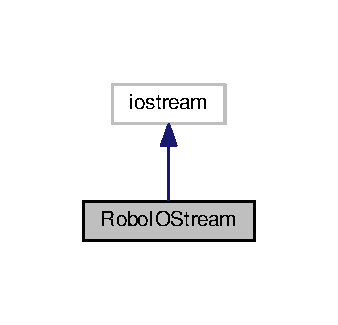
\includegraphics[width=162pt]{classRoboIOStream__inherit__graph}
\end{center}
\end{figure}


Collaboration diagram for Robo\+I\+O\+Stream\+:\nopagebreak
\begin{figure}[H]
\begin{center}
\leavevmode
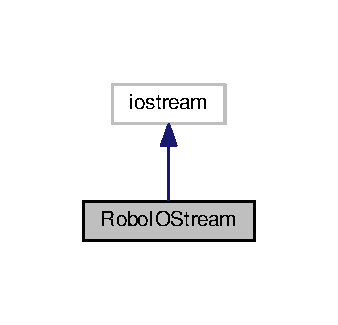
\includegraphics[width=162pt]{classRoboIOStream__coll__graph}
\end{center}
\end{figure}


The documentation for this class was generated from the following file\+:\begin{DoxyCompactItemize}
\item 
include/gmolmodel/Robo\+I\+O\+Stream.\+hpp\end{DoxyCompactItemize}

\hypertarget{classSampler}{}\section{Sampler Class Reference}
\label{classSampler}\index{Sampler@{Sampler}}


Inheritance diagram for Sampler\+:\nopagebreak
\begin{figure}[H]
\begin{center}
\leavevmode
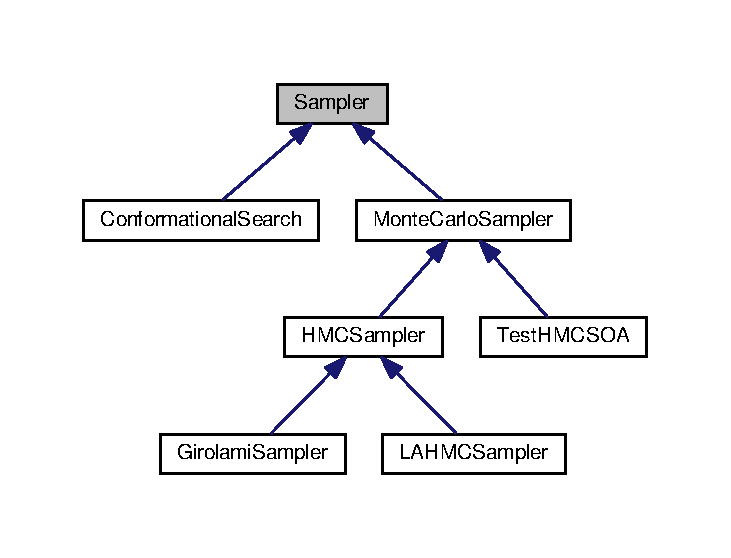
\includegraphics[width=350pt]{classSampler__inherit__graph}
\end{center}
\end{figure}


Collaboration diagram for Sampler\+:\nopagebreak
\begin{figure}[H]
\begin{center}
\leavevmode
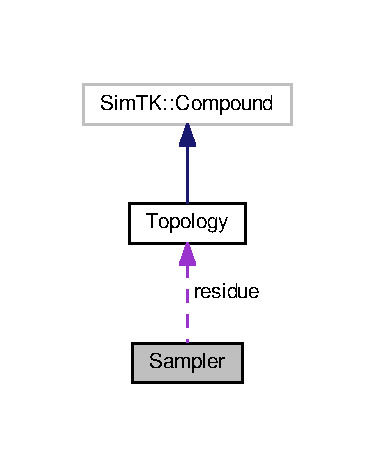
\includegraphics[width=180pt]{classSampler__coll__graph}
\end{center}
\end{figure}
\subsection*{Public Member Functions}
\begin{DoxyCompactItemize}
\item 
{\bfseries Sampler} (Sim\+T\+K\+::\+Compound\+System $\ast$arg\+Compound\+System, Sim\+T\+K\+::\+Simbody\+Matter\+Subsystem $\ast$arg\+Matter, std\+::vector$<$ \hyperlink{classTopology}{Topology} $\ast$ $>$ \&arg\+Topologies, Sim\+T\+K\+::\+Du\+M\+M\+Force\+Field\+Subsystem $\ast$arg\+Dumm, Sim\+T\+K\+::\+General\+Force\+Subsystem $\ast$forces, Sim\+T\+K\+::\+Time\+Stepper $\ast$arg\+Time\+Stepper)\hypertarget{classSampler_a1ff6da3170a6c479e3f61adcee82ae66}{}\label{classSampler_a1ff6da3170a6c479e3f61adcee82ae66}

\item 
Sim\+T\+K\+::\+Real {\bfseries calc\+Mass\+Determinant} (const Sim\+T\+K\+::\+State \&)\hypertarget{classSampler_a26ca57993693da9033b38474cc94a656}{}\label{classSampler_a26ca57993693da9033b38474cc94a656}

\item 
Sim\+T\+K\+::\+Real {\bfseries calc\+Mass\+Determinant} (Sim\+T\+K\+::\+State \&)\hypertarget{classSampler_ab5d6291d8839ac6b3a8da456377e7226}{}\label{classSampler_ab5d6291d8839ac6b3a8da456377e7226}

\item 
void {\bfseries initialize} (Sim\+T\+K\+::\+State \&some\+State)\hypertarget{classSampler_a8dc03cad5d5ed1ad6e8308ed449fbb3c}{}\label{classSampler_a8dc03cad5d5ed1ad6e8308ed449fbb3c}

\item 
void {\bfseries reinitialize} (Sim\+T\+K\+::\+State \&some\+State)\hypertarget{classSampler_a2370ac1b2d92f333451ace593f658ce0}{}\label{classSampler_a2370ac1b2d92f333451ace593f658ce0}

\item 
Sim\+T\+K\+::\+Real {\bfseries get\+Temperature} () const \hypertarget{classSampler_a32e49d15db5f08ad4ab3ee7dfa75ed51}{}\label{classSampler_a32e49d15db5f08ad4ab3ee7dfa75ed51}

\item 
void \hyperlink{classSampler_a74cb9a03076df1c093806acd3178ba4f}{set\+Temperature} (Sim\+T\+K\+::\+Real temperature)
\item 
Sim\+T\+K\+::\+Real {\bfseries get\+RT} () const \hypertarget{classSampler_a3ebad4cf7047e90a7f826c2c4b8e01e2}{}\label{classSampler_a3ebad4cf7047e90a7f826c2c4b8e01e2}

\item 
void \hyperlink{classSampler_a3c0cbd43a89ee644ac462e3609c1d578}{set\+Beta} (Sim\+T\+K\+::\+Real arg\+Beta)
\item 
Sim\+T\+K\+::\+Real {\bfseries get\+Beta} () const \hypertarget{classSampler_aa811d3879623dfd9c855a8777b026a08}{}\label{classSampler_aa811d3879623dfd9c855a8777b026a08}

\item 
void \hyperlink{classSampler_a1e71eaf9562ef25a8dc27c53ca5e93f4}{load\+Mbx2mobility} (Sim\+T\+K\+::\+State \&some\+State)
\item 
int \hyperlink{classSampler_af3dfbb0921f97da86d0b0c3e51d58a47}{get\+Nof\+Samples} (void)
\item 
unsigned long long int {\bfseries get\+Seed} (void)\hypertarget{classSampler_a5ba75a69456c27778dcdb999169a0c0f}{}\label{classSampler_a5ba75a69456c27778dcdb999169a0c0f}

\item 
void \hyperlink{classSampler_ac9292ab10f2c4dd3a3626bab9819c923}{set\+Seed} (unsigned long long int)
\item 
Sim\+T\+K\+::\+Real \hyperlink{classSampler_a9d4455f6786a507dc856dd16117122d9}{generate\+Random\+Number} (Gmol\+Rand\+Distribution\+Type)
\item 
virtual void \hyperlink{classSampler_a3022d2efacf6107b3fba506d31e2919e}{propose} (Sim\+T\+K\+::\+State \&some\+State)=0
\item 
virtual void {\bfseries update} (Sim\+T\+K\+::\+State \&some\+State)=0\hypertarget{classSampler_a4887b45db93b240608a90712f856df69}{}\label{classSampler_a4887b45db93b240608a90712f856df69}

\item 
void {\bfseries Print\+Simbody\+State\+Cache} (Sim\+T\+K\+::\+State \&some\+State)\hypertarget{classSampler_abe095828aebb30121068fc338d0b43e0}{}\label{classSampler_abe095828aebb30121068fc338d0b43e0}

\end{DoxyCompactItemize}
\subsection*{Public Attributes}
\begin{DoxyCompactItemize}
\item 
const Sim\+T\+K\+::\+System $\ast$ {\bfseries system}\hypertarget{classSampler_a25c66070f64d79e8b94c678b78d0e277}{}\label{classSampler_a25c66070f64d79e8b94c678b78d0e277}

\item 
Sim\+T\+K\+::\+Compound\+System $\ast$ {\bfseries compound\+System}\hypertarget{classSampler_aa9d5f0914ab6868559980ae0a7c3bd62}{}\label{classSampler_aa9d5f0914ab6868559980ae0a7c3bd62}

\item 
Sim\+T\+K\+::\+Simbody\+Matter\+Subsystem $\ast$ {\bfseries matter}\hypertarget{classSampler_a88113c1bcf12b6a11c6274697f6c186b}{}\label{classSampler_a88113c1bcf12b6a11c6274697f6c186b}

\item 
\hyperlink{classTopology}{Topology} $\ast$ {\bfseries residue}\hypertarget{classSampler_ad4577776a8e351803ccdceeeb9cc8f53}{}\label{classSampler_ad4577776a8e351803ccdceeeb9cc8f53}

\item 
std\+::vector$<$ \hyperlink{classTopology}{Topology} $\ast$ $>$ {\bfseries topologies}\hypertarget{classSampler_ac00c89482575d83ad879436effeddebc}{}\label{classSampler_ac00c89482575d83ad879436effeddebc}

\item 
int {\bfseries natoms}\hypertarget{classSampler_adfb71a546356d6e8f65aacb40aa98cfe}{}\label{classSampler_adfb71a546356d6e8f65aacb40aa98cfe}

\item 
int {\bfseries ndofs}\hypertarget{classSampler_ac261eb04d288ae674e9da7fa69e5af54}{}\label{classSampler_ac261eb04d288ae674e9da7fa69e5af54}

\item 
std\+::map$<$ Sim\+T\+K\+::\+Mobilized\+Body\+Index, Sim\+T\+K\+::\+Bond\+Mobility\+::\+Mobility $>$ \hyperlink{classSampler_a795db0c66f3527f447f899f552c30a8b}{mbx2mobility}
\item 
std\+::map$<$ Sim\+T\+K\+::\+Q\+Index, Joint\+Type $>$ {\bfseries q\+Index2joint\+Type}\hypertarget{classSampler_ad6bdd42c05c63d7f1ac17b170fb0745b}{}\label{classSampler_ad6bdd42c05c63d7f1ac17b170fb0745b}

\item 
Sim\+T\+K\+::\+Du\+M\+M\+Force\+Field\+Subsystem $\ast$ {\bfseries dumm}\hypertarget{classSampler_a87dbe61f06ba47644bd77d397fc505a2}{}\label{classSampler_a87dbe61f06ba47644bd77d397fc505a2}

\item 
Sim\+T\+K\+::\+General\+Force\+Subsystem $\ast$ {\bfseries forces}\hypertarget{classSampler_ac6fd8324ef573b7fd765ae572ee06343}{}\label{classSampler_ac6fd8324ef573b7fd765ae572ee06343}

\item 
Sim\+T\+K\+::\+Time\+Stepper $\ast$ {\bfseries time\+Stepper}\hypertarget{classSampler_a25ad4e02e2fcb4c8aaf914a678dee128}{}\label{classSampler_a25ad4e02e2fcb4c8aaf914a678dee128}

\item 
Thermostat\+Name {\bfseries thermostat}\hypertarget{classSampler_a464e1c642da90803d760265d2904c765}{}\label{classSampler_a464e1c642da90803d760265d2904c765}

\item 
Sim\+T\+K\+::\+Real {\bfseries temperature}\hypertarget{classSampler_a5bdd4b90cf4dec04e4dc8cd900cc9857}{}\label{classSampler_a5bdd4b90cf4dec04e4dc8cd900cc9857}

\item 
Sim\+T\+K\+::\+Real {\bfseries RT}\hypertarget{classSampler_a6ec4ff10320afbba1db255f691bcdbbd}{}\label{classSampler_a6ec4ff10320afbba1db255f691bcdbbd}

\item 
Sim\+T\+K\+::\+Real {\bfseries beta}\hypertarget{classSampler_a67faf89e26a9f4ed809c2ccf49023ad5}{}\label{classSampler_a67faf89e26a9f4ed809c2ccf49023ad5}

\item 
int {\bfseries nof\+Samples}\hypertarget{classSampler_aea870fef79a9d102e3da843b1455fbc3}{}\label{classSampler_aea870fef79a9d102e3da843b1455fbc3}

\item 
unsigned long long int {\bfseries seed}\hypertarget{classSampler_aaa55f25f620ba200654c52d1a50d27de}{}\label{classSampler_aaa55f25f620ba200654c52d1a50d27de}

\item 
bool {\bfseries acc}\hypertarget{classSampler_a97d8bc64196e61c2b86ed0d4fc8c669c}{}\label{classSampler_a97d8bc64196e61c2b86ed0d4fc8c669c}

\item 
boost\+::random\+::mt19937 {\bfseries random\+Engine} = boost\+::random\+::mt19937()\hypertarget{classSampler_a3abf6a00b9395c28ec428d9ca89794e0}{}\label{classSampler_a3abf6a00b9395c28ec428d9ca89794e0}

\item 
boost\+::random\+::uniform\+\_\+real\+\_\+distribution$<$ double $>$ {\bfseries uniform\+Real\+Distribution\+\_\+0\+\_\+2pi}
\item 
boost\+::random\+::uniform\+\_\+real\+\_\+distribution$<$ double $>$ {\bfseries uniform\+Real\+Distribution\+\_\+mpi\+\_\+pi}
\item 
boost\+::random\+::uniform\+\_\+real\+\_\+distribution$<$ double $>$ {\bfseries uniform\+Real\+Distribution}
\item 
boost\+::random\+::uniform\+\_\+real\+\_\+distribution$<$ double $>$ {\bfseries uniform\+Real\+Distribution\+\_\+m1\+\_\+1}
\item 
boost\+::normal\+\_\+distribution {\bfseries gaurand} = boost\+::normal\+\_\+distribution$<$$>$(0.\+0, 1.\+0)\hypertarget{classSampler_adc634e05a08e7937b1976c0b5ddb844d}{}\label{classSampler_adc634e05a08e7937b1976c0b5ddb844d}

\end{DoxyCompactItemize}


\subsection{Member Function Documentation}
\index{Sampler@{Sampler}!generate\+Random\+Number@{generate\+Random\+Number}}
\index{generate\+Random\+Number@{generate\+Random\+Number}!Sampler@{Sampler}}
\subsubsection[{\texorpdfstring{generate\+Random\+Number(\+Gmol\+Rand\+Distribution\+Type)}{generateRandomNumber(GmolRandDistributionType)}}]{\setlength{\rightskip}{0pt plus 5cm}Sim\+T\+K\+::\+Real Sampler\+::generate\+Random\+Number (
\begin{DoxyParamCaption}
\item[{Gmol\+Rand\+Distribution\+Type}]{distribution\+Type}
\end{DoxyParamCaption}
)}\hypertarget{classSampler_a9d4455f6786a507dc856dd16117122d9}{}\label{classSampler_a9d4455f6786a507dc856dd16117122d9}
Generate a random number. \index{Sampler@{Sampler}!get\+Nof\+Samples@{get\+Nof\+Samples}}
\index{get\+Nof\+Samples@{get\+Nof\+Samples}!Sampler@{Sampler}}
\subsubsection[{\texorpdfstring{get\+Nof\+Samples(void)}{getNofSamples(void)}}]{\setlength{\rightskip}{0pt plus 5cm}int Sampler\+::get\+Nof\+Samples (
\begin{DoxyParamCaption}
\item[{void}]{}
\end{DoxyParamCaption}
)}\hypertarget{classSampler_af3dfbb0921f97da86d0b0c3e51d58a47}{}\label{classSampler_af3dfbb0921f97da86d0b0c3e51d58a47}
Returns the number of samples extracted so far.

Returns the number of MC trials done by this integrator. \index{Sampler@{Sampler}!load\+Mbx2mobility@{load\+Mbx2mobility}}
\index{load\+Mbx2mobility@{load\+Mbx2mobility}!Sampler@{Sampler}}
\subsubsection[{\texorpdfstring{load\+Mbx2mobility(\+Sim\+T\+K\+::\+State \&some\+State)}{loadMbx2mobility(SimTK::State &someState)}}]{\setlength{\rightskip}{0pt plus 5cm}void Sampler\+::load\+Mbx2mobility (
\begin{DoxyParamCaption}
\item[{Sim\+T\+K\+::\+State \&}]{some\+State}
\end{DoxyParamCaption}
)}\hypertarget{classSampler_a1e71eaf9562ef25a8dc27c53ca5e93f4}{}\label{classSampler_a1e71eaf9562ef25a8dc27c53ca5e93f4}
Load the map of mobods to joint types $<$ Unrestricted bond, permitting changes in stretch, bend, and torsion modes

$<$ Bond has fixed length and angles, but permits rotation about the bond axis

$<$ Bond links both atoms to the same rigid unit

$<$ Three rotational dofs. It allows angle flexibility besides torsion.

$<$ Three rotational dofs. It allows angle flexibility besides torsion.

$<$ Torsion plus translation along the bond

$<$ Three translational mobilities (Cartesian). // N\+E\+W\+M\+OB

$<$ Three translational mobilities (Cartesian). // N\+E\+W\+M\+OB

$<$ Two rotational mobilities // N\+E\+W\+M\+OB

$<$ Two rotational mobilities // N\+E\+W\+M\+OB

$<$ Cap de bara

$<$ B\+AT coordinates

$<$ Translation along bond \index{Sampler@{Sampler}!propose@{propose}}
\index{propose@{propose}!Sampler@{Sampler}}
\subsubsection[{\texorpdfstring{propose(\+Sim\+T\+K\+::\+State \&some\+State)=0}{propose(SimTK::State &someState)=0}}]{\setlength{\rightskip}{0pt plus 5cm}virtual void Sampler\+::propose (
\begin{DoxyParamCaption}
\item[{Sim\+T\+K\+::\+State \&}]{some\+State}
\end{DoxyParamCaption}
)\hspace{0.3cm}{\ttfamily [pure virtual]}}\hypertarget{classSampler_a3022d2efacf6107b3fba506d31e2919e}{}\label{classSampler_a3022d2efacf6107b3fba506d31e2919e}
Propose a move 

Implemented in \hyperlink{classLAHMCSampler_aedb4b87feaaa20c036c908c9e9868b41}{L\+A\+H\+M\+C\+Sampler}, \hyperlink{classHMCSampler_aa36ab4482bbb6295658e8fe6a49c9e4f}{H\+M\+C\+Sampler}, \hyperlink{classMonteCarloSampler_af35ad7b12d462b867b968e3ec8194c05}{Monte\+Carlo\+Sampler}, and \hyperlink{classConformationalSearch_a1656b70ede0f43765c9379737d6e6697}{Conformational\+Search}.

\index{Sampler@{Sampler}!set\+Beta@{set\+Beta}}
\index{set\+Beta@{set\+Beta}!Sampler@{Sampler}}
\subsubsection[{\texorpdfstring{set\+Beta(\+Sim\+T\+K\+::\+Real arg\+Beta)}{setBeta(SimTK::Real argBeta)}}]{\setlength{\rightskip}{0pt plus 5cm}void Sampler\+::set\+Beta (
\begin{DoxyParamCaption}
\item[{Sim\+T\+K\+::\+Real}]{arg\+Beta}
\end{DoxyParamCaption}
)}\hypertarget{classSampler_a3c0cbd43a89ee644ac462e3609c1d578}{}\label{classSampler_a3c0cbd43a89ee644ac462e3609c1d578}
Setter for macroscopic beta. Also sets the RT and temperature \index{Sampler@{Sampler}!set\+Seed@{set\+Seed}}
\index{set\+Seed@{set\+Seed}!Sampler@{Sampler}}
\subsubsection[{\texorpdfstring{set\+Seed(unsigned long long int)}{setSeed(unsigned long long int)}}]{\setlength{\rightskip}{0pt plus 5cm}void Sampler\+::set\+Seed (
\begin{DoxyParamCaption}
\item[{unsigned long long int}]{arg\+Seed}
\end{DoxyParamCaption}
)}\hypertarget{classSampler_ac9292ab10f2c4dd3a3626bab9819c923}{}\label{classSampler_ac9292ab10f2c4dd3a3626bab9819c923}
Store the value of the seed internally and also feed it to the random number generator \index{Sampler@{Sampler}!set\+Temperature@{set\+Temperature}}
\index{set\+Temperature@{set\+Temperature}!Sampler@{Sampler}}
\subsubsection[{\texorpdfstring{set\+Temperature(\+Sim\+T\+K\+::\+Real temperature)}{setTemperature(SimTK::Real temperature)}}]{\setlength{\rightskip}{0pt plus 5cm}void Sampler\+::set\+Temperature (
\begin{DoxyParamCaption}
\item[{Sim\+T\+K\+::\+Real}]{temperature}
\end{DoxyParamCaption}
)}\hypertarget{classSampler_a74cb9a03076df1c093806acd3178ba4f}{}\label{classSampler_a74cb9a03076df1c093806acd3178ba4f}
Setter for macroscopic temperature. Also sets the RT and beta 

\subsection{Member Data Documentation}
\index{Sampler@{Sampler}!mbx2mobility@{mbx2mobility}}
\index{mbx2mobility@{mbx2mobility}!Sampler@{Sampler}}
\subsubsection[{\texorpdfstring{mbx2mobility}{mbx2mobility}}]{\setlength{\rightskip}{0pt plus 5cm}std\+::map$<$ Sim\+T\+K\+::\+Mobilized\+Body\+Index, Sim\+T\+K\+::\+Bond\+Mobility\+::\+Mobility$>$ Sampler\+::mbx2mobility}\hypertarget{classSampler_a795db0c66f3527f447f899f552c30a8b}{}\label{classSampler_a795db0c66f3527f447f899f552c30a8b}
Joint types \index{Sampler@{Sampler}!uniform\+Real\+Distribution@{uniform\+Real\+Distribution}}
\index{uniform\+Real\+Distribution@{uniform\+Real\+Distribution}!Sampler@{Sampler}}
\subsubsection[{\texorpdfstring{uniform\+Real\+Distribution}{uniformRealDistribution}}]{\setlength{\rightskip}{0pt plus 5cm}boost\+::random\+::uniform\+\_\+real\+\_\+distribution$<$double$>$ Sampler\+::uniform\+Real\+Distribution}\hypertarget{classSampler_a8f26cbe054715a164a8a0e0cc5226690}{}\label{classSampler_a8f26cbe054715a164a8a0e0cc5226690}
{\bfseries Initial value\+:}
\begin{DoxyCode}
=
            boost::random::uniform\_real\_distribution<double>(SimTK::Zero, SimTK::One)
\end{DoxyCode}
\index{Sampler@{Sampler}!uniform\+Real\+Distribution\+\_\+0\+\_\+2pi@{uniform\+Real\+Distribution\+\_\+0\+\_\+2pi}}
\index{uniform\+Real\+Distribution\+\_\+0\+\_\+2pi@{uniform\+Real\+Distribution\+\_\+0\+\_\+2pi}!Sampler@{Sampler}}
\subsubsection[{\texorpdfstring{uniform\+Real\+Distribution\+\_\+0\+\_\+2pi}{uniformRealDistribution_0_2pi}}]{\setlength{\rightskip}{0pt plus 5cm}boost\+::random\+::uniform\+\_\+real\+\_\+distribution$<$double$>$ Sampler\+::uniform\+Real\+Distribution\+\_\+0\+\_\+2pi}\hypertarget{classSampler_acf6ddd3830ce3ea8ac991f0d6c42325b}{}\label{classSampler_acf6ddd3830ce3ea8ac991f0d6c42325b}
{\bfseries Initial value\+:}
\begin{DoxyCode}
=
            boost::random::uniform\_real\_distribution<double>(SimTK::Zero, 2*SimTK::Pi)
\end{DoxyCode}
\index{Sampler@{Sampler}!uniform\+Real\+Distribution\+\_\+m1\+\_\+1@{uniform\+Real\+Distribution\+\_\+m1\+\_\+1}}
\index{uniform\+Real\+Distribution\+\_\+m1\+\_\+1@{uniform\+Real\+Distribution\+\_\+m1\+\_\+1}!Sampler@{Sampler}}
\subsubsection[{\texorpdfstring{uniform\+Real\+Distribution\+\_\+m1\+\_\+1}{uniformRealDistribution_m1_1}}]{\setlength{\rightskip}{0pt plus 5cm}boost\+::random\+::uniform\+\_\+real\+\_\+distribution$<$double$>$ Sampler\+::uniform\+Real\+Distribution\+\_\+m1\+\_\+1}\hypertarget{classSampler_aa05d95f8667613e9d802081ab343bc72}{}\label{classSampler_aa05d95f8667613e9d802081ab343bc72}
{\bfseries Initial value\+:}
\begin{DoxyCode}
=
            boost::random::uniform\_real\_distribution<double>((-1)*SimTK::One, SimTK::One)
\end{DoxyCode}
\index{Sampler@{Sampler}!uniform\+Real\+Distribution\+\_\+mpi\+\_\+pi@{uniform\+Real\+Distribution\+\_\+mpi\+\_\+pi}}
\index{uniform\+Real\+Distribution\+\_\+mpi\+\_\+pi@{uniform\+Real\+Distribution\+\_\+mpi\+\_\+pi}!Sampler@{Sampler}}
\subsubsection[{\texorpdfstring{uniform\+Real\+Distribution\+\_\+mpi\+\_\+pi}{uniformRealDistribution_mpi_pi}}]{\setlength{\rightskip}{0pt plus 5cm}boost\+::random\+::uniform\+\_\+real\+\_\+distribution$<$double$>$ Sampler\+::uniform\+Real\+Distribution\+\_\+mpi\+\_\+pi}\hypertarget{classSampler_a514a239abb55e5b7fb56d30fb2d1e695}{}\label{classSampler_a514a239abb55e5b7fb56d30fb2d1e695}
{\bfseries Initial value\+:}
\begin{DoxyCode}
=
            boost::random::uniform\_real\_distribution<double>((-1)*SimTK::Pi, SimTK::Pi)
\end{DoxyCode}


The documentation for this class was generated from the following files\+:\begin{DoxyCompactItemize}
\item 
include/gmolmodel/Sampler.\+hpp\item 
src/\hyperlink{Sampler_8cpp}{Sampler.\+cpp}\end{DoxyCompactItemize}

\hypertarget{classSetupReader}{}\section{Setup\+Reader Class Reference}
\label{classSetupReader}\index{Setup\+Reader@{Setup\+Reader}}


Inheritance diagram for Setup\+Reader\+:
\nopagebreak
\begin{figure}[H]
\begin{center}
\leavevmode
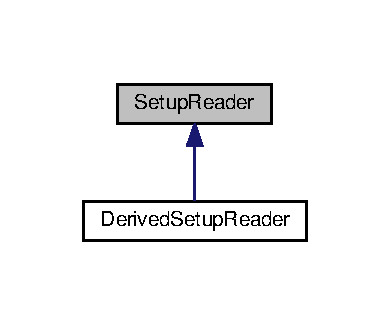
\includegraphics[width=187pt]{classSetupReader__inherit__graph}
\end{center}
\end{figure}
\subsection*{Public Member Functions}
\begin{DoxyCompactItemize}
\item 
{\bfseries Setup\+Reader} (const char $\ast$FN)\hypertarget{classSetupReader_abc7e894e1e1467fe04563d135459f3e5}{}\label{classSetupReader_abc7e894e1e1467fe04563d135459f3e5}

\item 
{\bfseries Setup\+Reader} (const std\+::string \&FN)\hypertarget{classSetupReader_a172ff7531a51c6471832531c2657b8b4}{}\label{classSetupReader_a172ff7531a51c6471832531c2657b8b4}

\item 
void {\bfseries Read\+Setup} (const char $\ast$FN)\hypertarget{classSetupReader_ac0d114a88ce4508719c52c50f773a6c9}{}\label{classSetupReader_ac0d114a88ce4508719c52c50f773a6c9}

\item 
void {\bfseries Read\+Setup} (const std\+::string \&FN)\hypertarget{classSetupReader_af746ca4e83e2d5e1f0174d2404351b8b}{}\label{classSetupReader_af746ca4e83e2d5e1f0174d2404351b8b}

\item 
void {\bfseries dump} (bool Pretty\+Print) const \hypertarget{classSetupReader_a1bd44ec38aac137acadce5b52427586b}{}\label{classSetupReader_a1bd44ec38aac137acadce5b52427586b}

\item 
bool \hyperlink{classSetupReader_a98207fe4240df790a2155368243006d5}{find} (const char $\ast$arg\+Key) const 
\item 
bool {\bfseries find} (const std\+::string \&arg\+Key) const \hypertarget{classSetupReader_a5cf206e3da57ffd8b84e30b38927945a}{}\label{classSetupReader_a5cf206e3da57ffd8b84e30b38927945a}

\item 
const std\+::vector$<$ std\+::string $>$ \& {\bfseries get} (const char $\ast$arg\+Key) const \hypertarget{classSetupReader_ab689005762b1d2c2e3ddd4d895f88fb6}{}\label{classSetupReader_ab689005762b1d2c2e3ddd4d895f88fb6}

\item 
const std\+::vector$<$ std\+::string $>$ \& {\bfseries get} (const std\+::string \&arg\+Key) const \hypertarget{classSetupReader_a68ff2717b1d1defb9ad8da4742513698}{}\label{classSetupReader_a68ff2717b1d1defb9ad8da4742513698}

\end{DoxyCompactItemize}


\subsection{Member Function Documentation}
\index{Setup\+Reader@{Setup\+Reader}!find@{find}}
\index{find@{find}!Setup\+Reader@{Setup\+Reader}}
\subsubsection[{\texorpdfstring{find(const char $\ast$arg\+Key) const }{find(const char *argKey) const }}]{\setlength{\rightskip}{0pt plus 5cm}bool Setup\+Reader\+::find (
\begin{DoxyParamCaption}
\item[{const char $\ast$}]{arg\+Key}
\end{DoxyParamCaption}
) const}\hypertarget{classSetupReader_a98207fe4240df790a2155368243006d5}{}\label{classSetupReader_a98207fe4240df790a2155368243006d5}
Check if key exists 

The documentation for this class was generated from the following files\+:\begin{DoxyCompactItemize}
\item 
include/gmolmodel/Setup\+Reader.\+hpp\item 
src/Setup\+Reader.\+cpp\end{DoxyCompactItemize}

\hypertarget{classTestHMCSOA}{}\section{Test\+H\+M\+C\+S\+OA Class Reference}
\label{classTestHMCSOA}\index{Test\+H\+M\+C\+S\+OA@{Test\+H\+M\+C\+S\+OA}}


Inheritance diagram for Test\+H\+M\+C\+S\+OA\+:\nopagebreak
\begin{figure}[H]
\begin{center}
\leavevmode
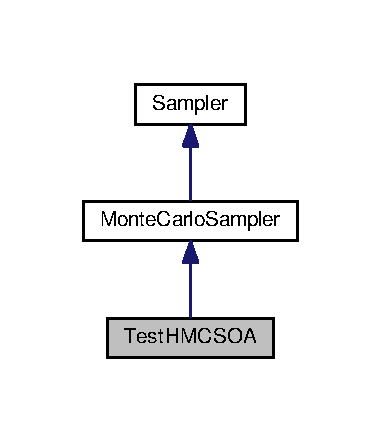
\includegraphics[width=183pt]{classTestHMCSOA__inherit__graph}
\end{center}
\end{figure}


Collaboration diagram for Test\+H\+M\+C\+S\+OA\+:\nopagebreak
\begin{figure}[H]
\begin{center}
\leavevmode
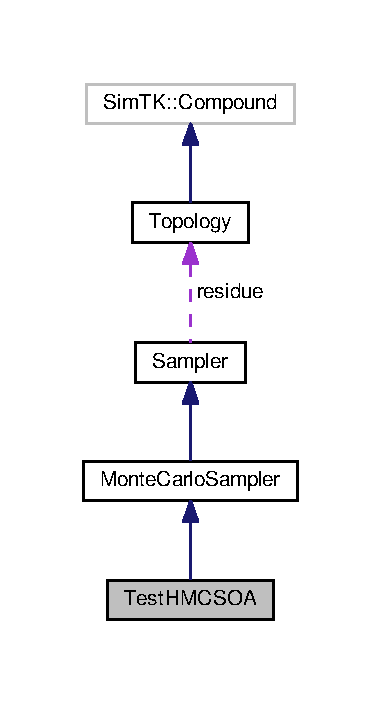
\includegraphics[width=183pt]{classTestHMCSOA__coll__graph}
\end{center}
\end{figure}
\subsection*{Public Member Functions}
\begin{DoxyCompactItemize}
\item 
{\bfseries Test\+H\+M\+C\+S\+OA} (Sim\+T\+K\+::\+Compound\+System $\ast$arg\+Compound\+System, Sim\+T\+K\+::\+Simbody\+Matter\+Subsystem $\ast$arg\+Matter, Sim\+T\+K\+::\+Compound $\ast$arg\+Residue, Sim\+T\+K\+::\+Du\+M\+M\+Force\+Field\+Subsystem $\ast$arg\+Dumm, Sim\+T\+K\+::\+General\+Force\+Subsystem $\ast$forces, Sim\+T\+K\+::\+Time\+Stepper $\ast$arg\+Time\+Stepper)\hypertarget{classTestHMCSOA_a2364faa39acdfbaf2c40b0029f8034ad}{}\label{classTestHMCSOA_a2364faa39acdfbaf2c40b0029f8034ad}

\item 
void {\bfseries calc\+Sqrt\+M\+InvL} (Sim\+T\+K\+::\+State \&some\+State, Sim\+T\+K\+::\+Matrix \&Sqrt\+M\+Inv)\hypertarget{classTestHMCSOA_a00b83f6d574017a27585bda53ebd2b85}{}\label{classTestHMCSOA_a00b83f6d574017a27585bda53ebd2b85}

\item 
void {\bfseries calc\+Sqrt\+M\+InvU} (Sim\+T\+K\+::\+State \&some\+State, Sim\+T\+K\+::\+Matrix \&Sqrt\+M\+Inv)\hypertarget{classTestHMCSOA_a9f33ac3396c3a50ae4d117128eb3c330}{}\label{classTestHMCSOA_a9f33ac3396c3a50ae4d117128eb3c330}

\item 
void {\bfseries calc\+Num\+Sqrt\+M\+Upper} (Sim\+T\+K\+::\+State \&some\+State, Sim\+T\+K\+::\+Matrix \&Sqrt\+M\+Upper)\hypertarget{classTestHMCSOA_acc16eb3051214df52691bdef5f8a54ea}{}\label{classTestHMCSOA_acc16eb3051214df52691bdef5f8a54ea}

\item 
virtual void {\bfseries initialize} (Sim\+T\+K\+::\+State \&advanced, Sim\+T\+K\+::\+Real timestep, int nosteps, Sim\+T\+K\+::\+Real arg\+Temperature, bool arg\+Use\+Fixman=true)\hypertarget{classTestHMCSOA_a8bdb352bb5fc093ba889dcb1c8dff1a6}{}\label{classTestHMCSOA_a8bdb352bb5fc093ba889dcb1c8dff1a6}

\item 
virtual void {\bfseries reinitialize} (Sim\+T\+K\+::\+State \&advanced, Sim\+T\+K\+::\+Real timestep, int nosteps, Sim\+T\+K\+::\+Real arg\+Temperature)\hypertarget{classTestHMCSOA_a7a483e9d2e14533e7bf24ea45d2424f7}{}\label{classTestHMCSOA_a7a483e9d2e14533e7bf24ea45d2424f7}

\item 
void {\bfseries propose} (Sim\+T\+K\+::\+State \&some\+State, Sim\+T\+K\+::\+Real timestep, int nosteps)\hypertarget{classTestHMCSOA_a50e579ed181768b081a68590701402d0}{}\label{classTestHMCSOA_a50e579ed181768b081a68590701402d0}

\item 
void {\bfseries update} (Sim\+T\+K\+::\+State \&some\+State, Sim\+T\+K\+::\+Real timestep, int nosteps)\hypertarget{classTestHMCSOA_a5d34a0c086770191eeedf656d882747a}{}\label{classTestHMCSOA_a5d34a0c086770191eeedf656d882747a}

\item 
Sim\+T\+K\+::\+Real {\bfseries get\+Old\+KE} (void)\hypertarget{classTestHMCSOA_a1ba6e3c9a65a90aa0c1bf47bd7660d22}{}\label{classTestHMCSOA_a1ba6e3c9a65a90aa0c1bf47bd7660d22}

\item 
Sim\+T\+K\+::\+Real {\bfseries get\+Set\+KE} (void)\hypertarget{classTestHMCSOA_ae6b420395d67a508ce6ca7ed4aeedaed}{}\label{classTestHMCSOA_ae6b420395d67a508ce6ca7ed4aeedaed}

\item 
void {\bfseries set\+Old\+KE} (Sim\+T\+K\+::\+Real)\hypertarget{classTestHMCSOA_adbcd426f3dd26ee69c3ac7acd8c7b8a3}{}\label{classTestHMCSOA_adbcd426f3dd26ee69c3ac7acd8c7b8a3}

\item 
void {\bfseries set\+Set\+KE} (Sim\+T\+K\+::\+Real)\hypertarget{classTestHMCSOA_a8c2d9beb09f282513fecd22da0fc95e1}{}\label{classTestHMCSOA_a8c2d9beb09f282513fecd22da0fc95e1}

\end{DoxyCompactItemize}
\subsection*{Protected Attributes}
\begin{DoxyCompactItemize}
\item 
Sim\+T\+K\+::\+Real {\bfseries ke\+\_\+set}\hypertarget{classTestHMCSOA_ab56809ea1f775e1b8e991d7a4db75b01}{}\label{classTestHMCSOA_ab56809ea1f775e1b8e991d7a4db75b01}

\item 
Sim\+T\+K\+::\+Real {\bfseries ke\+\_\+o}\hypertarget{classTestHMCSOA_a79b035979c103f97106f783924e963fa}{}\label{classTestHMCSOA_a79b035979c103f97106f783924e963fa}

\item 
Sim\+T\+K\+::\+Real {\bfseries etot\+\_\+set}\hypertarget{classTestHMCSOA_af04aa9201e9d3348f49bca5ddca734aa}{}\label{classTestHMCSOA_af04aa9201e9d3348f49bca5ddca734aa}

\item 
Sim\+T\+K\+::\+Real {\bfseries etot\+\_\+o}\hypertarget{classTestHMCSOA_a462dc02f4d80fe31eabbfbca0fd55946}{}\label{classTestHMCSOA_a462dc02f4d80fe31eabbfbca0fd55946}

\item 
Sim\+T\+K\+::\+Matrix {\bfseries prevM}\hypertarget{classTestHMCSOA_ae613b56cea287b2870a10034e0a5e664}{}\label{classTestHMCSOA_ae613b56cea287b2870a10034e0a5e664}

\item 
Sim\+T\+K\+::\+Real {\bfseries prev\+ThetaK}\hypertarget{classTestHMCSOA_ad3965ebb4116c89d3d43028b01322457}{}\label{classTestHMCSOA_ad3965ebb4116c89d3d43028b01322457}

\item 
Sim\+T\+K\+::\+Vector {\bfseries prev\+Theta}\hypertarget{classTestHMCSOA_acb6e5013a74bff45786d95f7ef00577b}{}\label{classTestHMCSOA_acb6e5013a74bff45786d95f7ef00577b}

\item 
Sim\+T\+K\+::\+Real {\bfseries prev\+Num\+DetM}\hypertarget{classTestHMCSOA_a87e8659d888b41db0d8e691003589682}{}\label{classTestHMCSOA_a87e8659d888b41db0d8e691003589682}

\item 
Sim\+T\+K\+::\+Real {\bfseries prev\+DetM}\hypertarget{classTestHMCSOA_a95ff59a5df94532f76bc4e2f0c61cf24}{}\label{classTestHMCSOA_a95ff59a5df94532f76bc4e2f0c61cf24}

\item 
int {\bfseries k\+For\+Theta}\hypertarget{classTestHMCSOA_ae0e68a6cc0093afcb198de88730a2200}{}\label{classTestHMCSOA_ae0e68a6cc0093afcb198de88730a2200}

\end{DoxyCompactItemize}
\subsection*{Additional Inherited Members}


The documentation for this class was generated from the following file\+:\begin{DoxyCompactItemize}
\item 
include/gmolmodel/H\+M\+C\+S\+O\+A.\+hpp\end{DoxyCompactItemize}

\hypertarget{classTopology}{}\section{Topology Class Reference}
\label{classTopology}\index{Topology@{Topology}}


{\ttfamily \#include $<$Topology.\+hpp$>$}



Inheritance diagram for Topology\+:\nopagebreak
\begin{figure}[H]
\begin{center}
\leavevmode
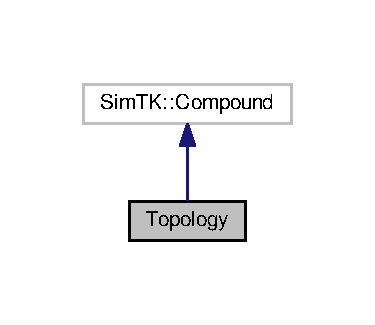
\includegraphics[width=180pt]{classTopology__inherit__graph}
\end{center}
\end{figure}


Collaboration diagram for Topology\+:\nopagebreak
\begin{figure}[H]
\begin{center}
\leavevmode
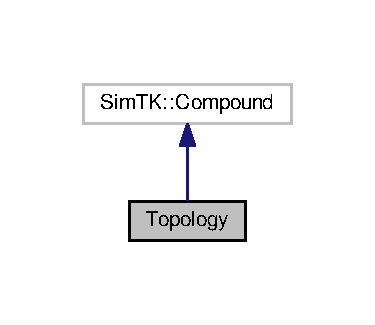
\includegraphics[width=180pt]{classTopology__coll__graph}
\end{center}
\end{figure}
\subsection*{Public Member Functions}
\begin{DoxyCompactItemize}
\item 
\hyperlink{classTopology_aa3336e10118cd76ab4b4c2ebc5062a9a}{Topology} ()
\item 
\hyperlink{classTopology_a6e001dfecb9782637eb17fc907f881cb}{Topology} (std\+::string name\+Of\+This\+Molecule)
\item 
virtual \hyperlink{classTopology_a3e447669757c8311c7f6f8edc705abf2}{$\sim$\+Topology} ()
\item 
void \hyperlink{classTopology_af73c991af8591ce8adaff56bcac66494}{Set\+Gmol\+Atom\+Properties\+From\+Reader} (\hyperlink{classreadAmberInput}{read\+Amber\+Input} $\ast$amber\+Reader)
\item 
void \hyperlink{classTopology_a84be38eb9b1dd5a689588dac50085947}{Set\+Gmol\+Bonding\+Properties\+From\+Reader} (\hyperlink{classreadAmberInput}{read\+Amber\+Input} $\ast$amber\+Reader)
\item 
void \hyperlink{classTopology_a84ca6201376207b20f1a6bc006f76bc8}{Set\+Gmol\+Atoms\+Molmodel\+Types} ()
\item 
void \hyperlink{classTopology_a0f0fa7fb6323767bb6db03fb1b74058c}{Set\+Gmol\+Atoms\+Molmodel\+Types\+Trial} ()
\item 
void \hyperlink{classTopology_a2127fe5e3df9f24bee960d15d4001ac4}{load\+Atom\+And\+Bond\+Info\+From\+Reader} (\hyperlink{classreadAmberInput}{read\+Amber\+Input} $\ast$amber\+Reader)
\item 
void \hyperlink{classTopology_a7083e732de18012caa11f9e5ea68c071}{Print\+Atom\+List} ()
\item 
void \hyperlink{classTopology_a6cd69af97ef2cadbfc66b12791821494}{b\+Add\+Biotypes} (std\+::string res\+Name, \hyperlink{classreadAmberInput}{read\+Amber\+Input} $\ast$amber\+Reader, Sim\+T\+K\+::\+Du\+M\+M\+Force\+Field\+Subsystem \&dumm)
\item 
void \hyperlink{classTopology_a4c6e17966e730dbc7972b1d060ae32aa}{b\+Add\+Atom\+Classes} (std\+::string res\+Name, \hyperlink{classreadAmberInput}{read\+Amber\+Input} $\ast$amber\+Reader, Sim\+T\+K\+::\+Du\+M\+M\+Force\+Field\+Subsystem \&dumm)
\item 
void \hyperlink{classTopology_adfe0053006ef2dfca18377d2c3726e3b}{b\+Add\+Bond\+Params} (std\+::string res\+Name, \hyperlink{classreadAmberInput}{read\+Amber\+Input} $\ast$amber\+Reader, Sim\+T\+K\+::\+Du\+M\+M\+Force\+Field\+Subsystem \&dumm)
\item 
void \hyperlink{classTopology_ac8b71a6aa2d8841cf2ad5f477eca2c70}{b\+Add\+Angle\+Params} (std\+::string res\+Name, \hyperlink{classreadAmberInput}{read\+Amber\+Input} $\ast$amber\+Reader, Sim\+T\+K\+::\+Du\+M\+M\+Force\+Field\+Subsystem \&dumm)
\item 
void \hyperlink{classTopology_ac082c73c8c91fa0f2c1d495f9e25f367}{b\+Add\+Torsion\+Params} (std\+::string res\+Name, \hyperlink{classreadAmberInput}{read\+Amber\+Input} $\ast$amber\+Reader, Sim\+T\+K\+::\+Du\+M\+M\+Force\+Field\+Subsystem \&dumm)
\item 
void \hyperlink{classTopology_a86ba17c55f8e311e0c0bcdba0c773da4}{b\+Add\+All\+Params} (\hyperlink{classreadAmberInput}{read\+Amber\+Input} $\ast$amber\+Reader, Sim\+T\+K\+::\+Du\+M\+M\+Force\+Field\+Subsystem \&dumm)
\item 
void \hyperlink{classTopology_a006cabf04e985e41f99b542904873ea0}{Print\+Molmodel\+And\+Du\+M\+M\+Types} (Sim\+T\+K\+::\+Du\+M\+M\+Force\+Field\+Subsystem \&dumm)
\item 
void \hyperlink{classTopology_a5a1fc33dd5965dd88f4e1b2d3f05b4dd}{build\+Acyclic\+Graph} (\hyperlink{classbSpecificAtom}{b\+Specific\+Atom} $\ast$node, \hyperlink{classbSpecificAtom}{b\+Specific\+Atom} $\ast$previous\+Node)
\item 
void \hyperlink{classTopology_a320ba4dbab67b1f1b810af4a23295143}{add\+Ring\+Closing\+Bonds} ()
\item 
void \hyperlink{classTopology_af493c145670b5362e58a17c87578fdb4}{match\+Default\+Configuration\+With\+Atom\+List} (Sim\+T\+K\+::\+Compound\+::\+Match\+Stratagem match\+Stratagem)
\item 
void \hyperlink{classTopology_a6185bfb169312e23495c94d54a06112e}{build\+Graph\+And\+Match\+Coords} (Sim\+T\+K\+::\+Du\+M\+M\+Force\+Field\+Subsystem \&dumm, int arg\+Root)
\item 
void \hyperlink{classTopology_a182953ce5f2024dc7a14cc68d4be8597}{set\+Flexibility} (std\+::string arg\+Regimen, std\+::string flex\+FN)
\item 
std\+::string \hyperlink{classTopology_a46d0c376fc14d523702db4e6c20d4311}{get\+Regimen} ()
\item 
const std\+::string \hyperlink{classTopology_a2c011e0bf248dd9329320e00fac4dcaa}{get\+Name} () const 
\item 
void \hyperlink{classTopology_ab94527095d261a020eec893e45c133fe}{set\+Name} (std\+::string name\+Of\+This\+Molecule)
\item 
const Sim\+T\+K\+::\+Compound\+System\+::\+Compound\+Index \& \hyperlink{classTopology_a8da806d0cc5d7e3c5debe6d48bd10d06}{get\+Compound\+Index} () const 
\item 
void \hyperlink{classTopology_a1a1124e3554ff2315926a54a0315fdbe}{set\+Compound\+Index} (const Sim\+T\+K\+::\+Compound\+System\+::\+Compound\+Index \&compound\+Index)
\item 
bool \hyperlink{classTopology_abf5a2669d0e20677eaadd6d87b2f8795}{check\+If\+Triple\+Unordered\+Are\+Equal} (std\+::vector$<$ Compound\+::\+Atom\+Index $>$ \&first, std\+::vector$<$ Compound\+::\+Atom\+Index $>$ \&second)
\item 
void {\bfseries load\+Triples} (void)\hypertarget{classTopology_a4b4022faf8d873713322e502821e9443}{}\label{classTopology_a4b4022faf8d873713322e502821e9443}

\item 
Sim\+T\+K\+::\+Real {\bfseries calc\+Log\+Sine\+Sqr\+Gamma2} (const Sim\+T\+K\+::\+State \&quat\+State)\hypertarget{classTopology_a35525d2a7aef61553490398165cbbfb8}{}\label{classTopology_a35525d2a7aef61553490398165cbbfb8}

\item 
Sim\+T\+K\+::\+Real {\bfseries calc\+Log\+Det\+M\+B\+A\+T\+Gamma2\+Contribution} (const Sim\+T\+K\+::\+State \&)\hypertarget{classTopology_aa6ce96a0e7660584b72f64d132f5a611}{}\label{classTopology_aa6ce96a0e7660584b72f64d132f5a611}

\item 
Sim\+T\+K\+::\+Real {\bfseries calc\+Log\+Det\+M\+B\+A\+T\+Dists\+Contribution} (const Sim\+T\+K\+::\+State \&)\hypertarget{classTopology_a50900405ea47b713fea6d12d046585db}{}\label{classTopology_a50900405ea47b713fea6d12d046585db}

\item 
Sim\+T\+K\+::\+Real {\bfseries calc\+Log\+Det\+M\+B\+A\+T\+Dists\+Masses\+Contribution} (const Sim\+T\+K\+::\+State \&)\hypertarget{classTopology_a20dbb8725aff8575fe6c889d714fb480}{}\label{classTopology_a20dbb8725aff8575fe6c889d714fb480}

\item 
Sim\+T\+K\+::\+Real {\bfseries calc\+Log\+Det\+M\+B\+A\+T\+Angles\+Contribution} (const Sim\+T\+K\+::\+State \&)\hypertarget{classTopology_a8a9060bb644aa335e2cbbb1e491388be}{}\label{classTopology_a8a9060bb644aa335e2cbbb1e491388be}

\item 
Sim\+T\+K\+::\+Real {\bfseries calc\+Log\+Det\+M\+B\+A\+T\+Masses\+Contribution} (const Sim\+T\+K\+::\+State \&)\hypertarget{classTopology_a466dfbf5b7c76d21f8c1261db415a445}{}\label{classTopology_a466dfbf5b7c76d21f8c1261db415a445}

\item 
Sim\+T\+K\+::\+Real {\bfseries calc\+Log\+Det\+M\+B\+A\+T\+Internal} (const Sim\+T\+K\+::\+State \&some\+State)\hypertarget{classTopology_ade491b23d6e41abbc84e809be14cd543}{}\label{classTopology_ade491b23d6e41abbc84e809be14cd543}

\item 
Sim\+T\+K\+::\+Real {\bfseries calc\+Log\+Det\+M\+B\+AT} (const Sim\+T\+K\+::\+State \&)\hypertarget{classTopology_a975172cc0f81baad15f67900b6fc517d}{}\label{classTopology_a975172cc0f81baad15f67900b6fc517d}

\item 
int \hyperlink{classTopology_a1725652fdbf27bcbda7e16c07bddc7b1}{get\+N\+Atoms} () const 
\item 
int \hyperlink{classTopology_aae1c39ba234dfa5df80a46f8009cd164}{get\+N\+Bonds} () const 
\item 
\hyperlink{classbSpecificAtom}{b\+Specific\+Atom} $\ast$ \hyperlink{classTopology_a5733e1f7ab0c145a05fdb9650d0d015a}{get\+Atom\+By\+Number} (int number) const 
\item 
\hyperlink{classbSpecificAtom}{b\+Specific\+Atom} $\ast$ \hyperlink{classTopology_a85f201c9fbb2164e57a13b2500b3a166}{upd\+Atom\+By\+Atom\+Ix} (int a\+Ix)
\item 
\hyperlink{classbSpecificAtom}{b\+Specific\+Atom} $\ast$ \hyperlink{classTopology_a87a161d4a1260c148eecc46682a1c664}{get\+Atom\+By\+Name} (std\+::string name) const 
\item 
std\+::vector$<$ \hyperlink{classbSpecificAtom}{b\+Specific\+Atom} $\ast$ $>$ \hyperlink{classTopology_ae1e1834b0011f578fc98a82fb544054b}{get\+Neighbours} (int) const 
\item 
Sim\+T\+K\+::\+Compound\+::\+Atom\+Index \hyperlink{classTopology_a0ce3bb644b6420d011b34b77ecb8567f}{get\+Chemical\+Parent} (Sim\+T\+K\+::\+Simbody\+Matter\+Subsystem $\ast$matter, Sim\+T\+K\+::\+Compound\+::\+Atom\+Index)
\item 
std\+::vector$<$ Sim\+T\+K\+::\+Transform $>$ {\bfseries calc\+Mobod\+Transforms} (Sim\+T\+K\+::\+Simbody\+Matter\+Subsystem $\ast$matter, Sim\+T\+K\+::\+Compound\+::\+Atom\+Index root\+Atom, const Sim\+T\+K\+::\+State \&some\+State)\hypertarget{classTopology_a685282e19f5f256a01edfbd295ea4e4b}{}\label{classTopology_a685282e19f5f256a01edfbd295ea4e4b}

\item 
void \hyperlink{classTopology_a4ed164b1fe5ece6e00a841bffe1861fa}{calc\+Top\+Transforms} (void)
\item 
void {\bfseries print\+Top\+Transforms} (void)\hypertarget{classTopology_a7108a6b3cdf56149fe38e1069f3e335c}{}\label{classTopology_a7108a6b3cdf56149fe38e1069f3e335c}

\item 
Sim\+T\+K\+::\+Transform {\bfseries get\+Top\+Transform} (Sim\+T\+K\+::\+Compound\+::\+Atom\+Index)\hypertarget{classTopology_a435cc596dae34536a0077c2ccb8c3827}{}\label{classTopology_a435cc596dae34536a0077c2ccb8c3827}

\item 
const \hyperlink{classbBond}{b\+Bond} \& {\bfseries get\+Bond} (int, int) const \hypertarget{classTopology_a98848edae3b427c123c2670b56084756}{}\label{classTopology_a98848edae3b427c123c2670b56084756}

\item 
int \hyperlink{classTopology_ac3cd9ae97a9ff8067de8486a1de6496d}{get\+Bond\+Order} (int, int) const 
\item 
std\+::map$<$ Sim\+T\+K\+::\+Mobilized\+Body\+Index, Sim\+T\+K\+::\+Compound\+::\+Atom\+Index $>$ \hyperlink{classTopology_a235216eef91888bb91491d0d40101e47}{get\+Mbx2a\+Ix} ()
\item 
std\+::map$<$ Sim\+T\+K\+::\+Compound\+::\+Atom\+Index, Sim\+T\+K\+::\+Mobilized\+Body\+Index $>$ \hyperlink{classTopology_a9e74d153cd138a14a21f94c449fc2319}{get\+A\+Ix2mbx} ()
\item 
unsigned int \hyperlink{classTopology_afdd58989b6c82c30b9bacaa9d697b513}{get\+Nof\+Mobilized\+Bodies} ()
\item 
void \hyperlink{classTopology_aff039c90beda2dc6f6437251ae5b67cd}{write\+Atom\+List\+Pdb} (std\+::string dirname, std\+::string prefix, std\+::string sufix, int max\+Nof\+Digits, int index) const 
\item 
void \hyperlink{classTopology_a182b8885b2e1fdda870e564d4b1d6abe}{load\+Mobods\+Related\+Maps} ()
\item 
void \hyperlink{classTopology_aea00ed376f65fb204651b35883a3573d}{load\+Compound\+Atom\+Ix2\+Gmol\+Atom\+Ix} (void)
\item 
int {\bfseries get\+Number} (Sim\+T\+K\+::\+Compound\+::\+Atom\+Index)\hypertarget{classTopology_a17db78e48fd9adcf78fa5a9fd0a3b62b}{}\label{classTopology_a17db78e48fd9adcf78fa5a9fd0a3b62b}

\item 
void \hyperlink{classTopology_af21777f1399571c3a13e91969a33b740}{print\+Maps} ()
\item 
void \hyperlink{classTopology_a6b97df7d3c33275e2a5008f3155c2242}{get\+Coordinates} (std\+::vector$<$ Sim\+T\+K\+::\+Real $>$ Xs, std\+::vector$<$ Sim\+T\+K\+::\+Real $>$ Ys, std\+::vector$<$ Sim\+T\+K\+::\+Real $>$ Zs)
\end{DoxyCompactItemize}
\subsection*{Public Attributes}
\begin{DoxyCompactItemize}
\item 
int {\bfseries natoms}\hypertarget{classTopology_ab37d7bfd8071b37fadcab2240a09a70f}{}\label{classTopology_ab37d7bfd8071b37fadcab2240a09a70f}

\item 
std\+::vector$<$ \hyperlink{classbSpecificAtom}{b\+Specific\+Atom} $>$ {\bfseries b\+Atom\+List}\hypertarget{classTopology_a0dc44c74b9b1b34969a0dbdfcba01c5c}{}\label{classTopology_a0dc44c74b9b1b34969a0dbdfcba01c5c}

\item 
int {\bfseries nbonds}\hypertarget{classTopology_ac820bfb62c44bed210c25f3f5de1f249}{}\label{classTopology_ac820bfb62c44bed210c25f3f5de1f249}

\item 
std\+::vector$<$ \hyperlink{classbBond}{b\+Bond} $>$ {\bfseries bonds}\hypertarget{classTopology_a50b082ce708c2649e8565c78dcc5fb26}{}\label{classTopology_a50b082ce708c2649e8565c78dcc5fb26}

\item 
int {\bfseries n\+Triples}\hypertarget{classTopology_ac6249044e82bec9fe7fb4e3231be890c}{}\label{classTopology_ac6249044e82bec9fe7fb4e3231be890c}

\item 
std\+::vector$<$ std\+::vector$<$ Compound\+::\+Atom\+Index $>$ $>$ {\bfseries triples}\hypertarget{classTopology_a36327556d21652f41d8909d4600cbd22}{}\label{classTopology_a36327556d21652f41d8909d4600cbd22}

\item 
std\+::map$<$ Sim\+T\+K\+::\+Mobilized\+Body\+Index, Sim\+T\+K\+::\+Compound\+::\+Atom\+Index $>$ {\bfseries mbx2a\+Ix}\hypertarget{classTopology_aa8d85a909e7c1b6a4d5873c338fcf471}{}\label{classTopology_aa8d85a909e7c1b6a4d5873c338fcf471}

\item 
std\+::map$<$ Sim\+T\+K\+::\+Compound\+::\+Atom\+Index, Sim\+T\+K\+::\+Mobilized\+Body\+Index $>$ {\bfseries a\+Ix2mbx}\hypertarget{classTopology_a4a5d3182210d2dbd78e5653044ceafee}{}\label{classTopology_a4a5d3182210d2dbd78e5653044ceafee}

\item 
std\+::map$<$ Sim\+T\+K\+::\+Compound\+::\+Atom\+Index, Sim\+T\+K\+::\+Transform $>$ {\bfseries a\+Ix2\+Top\+Transform}\hypertarget{classTopology_a6049ad3ebf58010d60371b79d2b4bff7}{}\label{classTopology_a6049ad3ebf58010d60371b79d2b4bff7}

\item 
std\+::map$<$ Sim\+T\+K\+::\+Compound\+::\+Atom\+Index, int $>$ {\bfseries Compound\+Atom\+Ix2\+Gmol\+Atom\+Ix}\hypertarget{classTopology_adfc3264e9a0ec7b0f3b6c72202569d0e}{}\label{classTopology_adfc3264e9a0ec7b0f3b6c72202569d0e}

\end{DoxyCompactItemize}


\subsection{Detailed Description}
Topological information (bonds graph) for one molecule. It maps to one compound in Molmodel thus it is derived from Molmodel Compound class. It does the following things\+:
\begin{DoxyItemize}
\item loads information from input files such as Amber input prmtop / inpcrd
\item adds parameters to a Du\+MM force field which belongs to the \hyperlink{classWorld}{World} class because one Du\+MM class should be used for multiple molecules
\item contructs the graph based on a list of \hyperlink{classbSpecificAtom}{b\+Specific\+Atom} objects each of which already contains bonding information from the input files
\item defines the rigid bodies based on imput files provided by the users. Contains a list of atoms b\+Atom\+List which consists of \hyperlink{classbSpecificAtom}{b\+Specific\+Atom} objects 
\end{DoxyItemize}

\subsection{Constructor \& Destructor Documentation}
\index{Topology@{Topology}!Topology@{Topology}}
\index{Topology@{Topology}!Topology@{Topology}}
\subsubsection[{\texorpdfstring{Topology()}{Topology()}}]{\setlength{\rightskip}{0pt plus 5cm}Topology\+::\+Topology (
\begin{DoxyParamCaption}
{}
\end{DoxyParamCaption}
)}\hypertarget{classTopology_aa3336e10118cd76ab4b4c2ebc5062a9a}{}\label{classTopology_aa3336e10118cd76ab4b4c2ebc5062a9a}
Default Constructor. Sets the name of this molecule to \textquotesingle{}no\+\_\+name \textquotesingle{}. The name has no particular function and is not guaranteed to be unique.

Default constructor.\+Sets the name of this molecule to \textquotesingle{}no\+\_\+name \textquotesingle{}. The name has no particular function and is not guaranteed to be unique \index{Topology@{Topology}!Topology@{Topology}}
\index{Topology@{Topology}!Topology@{Topology}}
\subsubsection[{\texorpdfstring{Topology(std\+::string name\+Of\+This\+Molecule)}{Topology(std::string nameOfThisMolecule)}}]{\setlength{\rightskip}{0pt plus 5cm}Topology\+::\+Topology (
\begin{DoxyParamCaption}
\item[{std\+::string}]{name\+Of\+This\+Molecule}
\end{DoxyParamCaption}
)\hspace{0.3cm}{\ttfamily [explicit]}}\hypertarget{classTopology_a6e001dfecb9782637eb17fc907f881cb}{}\label{classTopology_a6e001dfecb9782637eb17fc907f881cb}
Constructor that sets the name of the molecule. The name has no particular function and is not guaranteed to be unique.

Constructor that sets the name of the molecule. The name has no particular function and is not guaranteed to be unique \index{Topology@{Topology}!````~Topology@{$\sim$\+Topology}}
\index{````~Topology@{$\sim$\+Topology}!Topology@{Topology}}
\subsubsection[{\texorpdfstring{$\sim$\+Topology()}{~Topology()}}]{\setlength{\rightskip}{0pt plus 5cm}Topology\+::$\sim$\+Topology (
\begin{DoxyParamCaption}
{}
\end{DoxyParamCaption}
)\hspace{0.3cm}{\ttfamily [virtual]}}\hypertarget{classTopology_a3e447669757c8311c7f6f8edc705abf2}{}\label{classTopology_a3e447669757c8311c7f6f8edc705abf2}
Default Destructor.

Default destructor. It deallocates b\+Atom\+Type of every atom in the b\+Atom\+List because we want to allow the valence to change during the simulation e.\+g. semi-\/grand canonical ensemble. 

\subsection{Member Function Documentation}
\index{Topology@{Topology}!add\+Ring\+Closing\+Bonds@{add\+Ring\+Closing\+Bonds}}
\index{add\+Ring\+Closing\+Bonds@{add\+Ring\+Closing\+Bonds}!Topology@{Topology}}
\subsubsection[{\texorpdfstring{add\+Ring\+Closing\+Bonds()}{addRingClosingBonds()}}]{\setlength{\rightskip}{0pt plus 5cm}void Topology\+::add\+Ring\+Closing\+Bonds (
\begin{DoxyParamCaption}
{}
\end{DoxyParamCaption}
)}\hypertarget{classTopology_a320ba4dbab67b1f1b810af4a23295143}{}\label{classTopology_a320ba4dbab67b1f1b810af4a23295143}
After building the acyclic molecular tree close the remaining bonds \index{Topology@{Topology}!b\+Add\+All\+Params@{b\+Add\+All\+Params}}
\index{b\+Add\+All\+Params@{b\+Add\+All\+Params}!Topology@{Topology}}
\subsubsection[{\texorpdfstring{b\+Add\+All\+Params(read\+Amber\+Input $\ast$amber\+Reader, Sim\+T\+K\+::\+Du\+M\+M\+Force\+Field\+Subsystem \&dumm)}{bAddAllParams(readAmberInput *amberReader, SimTK::DuMMForceFieldSubsystem &dumm)}}]{\setlength{\rightskip}{0pt plus 5cm}void Topology\+::b\+Add\+All\+Params (
\begin{DoxyParamCaption}
\item[{{\bf read\+Amber\+Input} $\ast$}]{amber\+Reader, }
\item[{Sim\+T\+K\+::\+Du\+M\+M\+Force\+Field\+Subsystem \&}]{dumm}
\end{DoxyParamCaption}
)}\hypertarget{classTopology_a86ba17c55f8e311e0c0bcdba0c773da4}{}\label{classTopology_a86ba17c55f8e311e0c0bcdba0c773da4}
Adds force field parameters read by the input\+Reader to Du\+MM

Adds force field parameters read by the input\+Reader \index{Topology@{Topology}!b\+Add\+Angle\+Params@{b\+Add\+Angle\+Params}}
\index{b\+Add\+Angle\+Params@{b\+Add\+Angle\+Params}!Topology@{Topology}}
\subsubsection[{\texorpdfstring{b\+Add\+Angle\+Params(std\+::string res\+Name, read\+Amber\+Input $\ast$amber\+Reader, Sim\+T\+K\+::\+Du\+M\+M\+Force\+Field\+Subsystem \&dumm)}{bAddAngleParams(std::string resName, readAmberInput *amberReader, SimTK::DuMMForceFieldSubsystem &dumm)}}]{\setlength{\rightskip}{0pt plus 5cm}void Topology\+::b\+Add\+Angle\+Params (
\begin{DoxyParamCaption}
\item[{std\+::string}]{res\+Name, }
\item[{{\bf read\+Amber\+Input} $\ast$}]{amber\+Reader, }
\item[{Sim\+T\+K\+::\+Du\+M\+M\+Force\+Field\+Subsystem \&}]{dumm}
\end{DoxyParamCaption}
)}\hypertarget{classTopology_ac8b71a6aa2d8841cf2ad5f477eca2c70}{}\label{classTopology_ac8b71a6aa2d8841cf2ad5f477eca2c70}
Calls Du\+MM define\+Bond\+Bend.

Calls Du\+MM define\+Bond\+Bend to define angle parameters. \index{Topology@{Topology}!b\+Add\+Atom\+Classes@{b\+Add\+Atom\+Classes}}
\index{b\+Add\+Atom\+Classes@{b\+Add\+Atom\+Classes}!Topology@{Topology}}
\subsubsection[{\texorpdfstring{b\+Add\+Atom\+Classes(std\+::string res\+Name, read\+Amber\+Input $\ast$amber\+Reader, Sim\+T\+K\+::\+Du\+M\+M\+Force\+Field\+Subsystem \&dumm)}{bAddAtomClasses(std::string resName, readAmberInput *amberReader, SimTK::DuMMForceFieldSubsystem &dumm)}}]{\setlength{\rightskip}{0pt plus 5cm}void Topology\+::b\+Add\+Atom\+Classes (
\begin{DoxyParamCaption}
\item[{std\+::string}]{res\+Name, }
\item[{{\bf read\+Amber\+Input} $\ast$}]{amber\+Reader, }
\item[{Sim\+T\+K\+::\+Du\+M\+M\+Force\+Field\+Subsystem \&}]{dumm}
\end{DoxyParamCaption}
)}\hypertarget{classTopology_a4c6e17966e730dbc7972b1d060ae32aa}{}\label{classTopology_a4c6e17966e730dbc7972b1d060ae32aa}
It calls Du\+M\+Ms define\+Atom\+Class, define\+Charged\+Atom\+Tye and set\+Biotype\+Charged\+Atom\+Type for every atom. These Molmodel functions contain information regarding the force field parameters. \index{Topology@{Topology}!b\+Add\+Biotypes@{b\+Add\+Biotypes}}
\index{b\+Add\+Biotypes@{b\+Add\+Biotypes}!Topology@{Topology}}
\subsubsection[{\texorpdfstring{b\+Add\+Biotypes(std\+::string res\+Name, read\+Amber\+Input $\ast$amber\+Reader, Sim\+T\+K\+::\+Du\+M\+M\+Force\+Field\+Subsystem \&dumm)}{bAddBiotypes(std::string resName, readAmberInput *amberReader, SimTK::DuMMForceFieldSubsystem &dumm)}}]{\setlength{\rightskip}{0pt plus 5cm}void Topology\+::b\+Add\+Biotypes (
\begin{DoxyParamCaption}
\item[{std\+::string}]{res\+Name, }
\item[{{\bf read\+Amber\+Input} $\ast$}]{amber\+Reader, }
\item[{Sim\+T\+K\+::\+Du\+M\+M\+Force\+Field\+Subsystem \&}]{dumm}
\end{DoxyParamCaption}
)}\hypertarget{classTopology_a6cd69af97ef2cadbfc66b12791821494}{}\label{classTopology_a6cd69af97ef2cadbfc66b12791821494}
Biotype is a Molmodel hook that is usually used to look up molecular force field specific parameters for an atom type. Gmolmodel defines a new Biotype for each atom. The only thing that is specified is the element with info about name, atomic number, valence and mass. \index{Topology@{Topology}!b\+Add\+Bond\+Params@{b\+Add\+Bond\+Params}}
\index{b\+Add\+Bond\+Params@{b\+Add\+Bond\+Params}!Topology@{Topology}}
\subsubsection[{\texorpdfstring{b\+Add\+Bond\+Params(std\+::string res\+Name, read\+Amber\+Input $\ast$amber\+Reader, Sim\+T\+K\+::\+Du\+M\+M\+Force\+Field\+Subsystem \&dumm)}{bAddBondParams(std::string resName, readAmberInput *amberReader, SimTK::DuMMForceFieldSubsystem &dumm)}}]{\setlength{\rightskip}{0pt plus 5cm}void Topology\+::b\+Add\+Bond\+Params (
\begin{DoxyParamCaption}
\item[{std\+::string}]{res\+Name, }
\item[{{\bf read\+Amber\+Input} $\ast$}]{amber\+Reader, }
\item[{Sim\+T\+K\+::\+Du\+M\+M\+Force\+Field\+Subsystem \&}]{dumm}
\end{DoxyParamCaption}
)}\hypertarget{classTopology_adfe0053006ef2dfca18377d2c3726e3b}{}\label{classTopology_adfe0053006ef2dfca18377d2c3726e3b}
Calls Du\+MM define\+Bond\+Stretch.

Calls Du\+MM define\+Bond\+Stretch to define bonds parameters. \index{Topology@{Topology}!b\+Add\+Torsion\+Params@{b\+Add\+Torsion\+Params}}
\index{b\+Add\+Torsion\+Params@{b\+Add\+Torsion\+Params}!Topology@{Topology}}
\subsubsection[{\texorpdfstring{b\+Add\+Torsion\+Params(std\+::string res\+Name, read\+Amber\+Input $\ast$amber\+Reader, Sim\+T\+K\+::\+Du\+M\+M\+Force\+Field\+Subsystem \&dumm)}{bAddTorsionParams(std::string resName, readAmberInput *amberReader, SimTK::DuMMForceFieldSubsystem &dumm)}}]{\setlength{\rightskip}{0pt plus 5cm}void Topology\+::b\+Add\+Torsion\+Params (
\begin{DoxyParamCaption}
\item[{std\+::string}]{res\+Name, }
\item[{{\bf read\+Amber\+Input} $\ast$}]{amber\+Reader, }
\item[{Sim\+T\+K\+::\+Du\+M\+M\+Force\+Field\+Subsystem \&}]{dumm}
\end{DoxyParamCaption}
)}\hypertarget{classTopology_ac082c73c8c91fa0f2c1d495f9e25f367}{}\label{classTopology_ac082c73c8c91fa0f2c1d495f9e25f367}
Calls Du\+MM define\+Bond\+Torsion for 1, 2 and 3 periodicities \index{Topology@{Topology}!build\+Acyclic\+Graph@{build\+Acyclic\+Graph}}
\index{build\+Acyclic\+Graph@{build\+Acyclic\+Graph}!Topology@{Topology}}
\subsubsection[{\texorpdfstring{build\+Acyclic\+Graph(b\+Specific\+Atom $\ast$node, b\+Specific\+Atom $\ast$previous\+Node)}{buildAcyclicGraph(bSpecificAtom *node, bSpecificAtom *previousNode)}}]{\setlength{\rightskip}{0pt plus 5cm}void Topology\+::build\+Acyclic\+Graph (
\begin{DoxyParamCaption}
\item[{{\bf b\+Specific\+Atom} $\ast$}]{node, }
\item[{{\bf b\+Specific\+Atom} $\ast$}]{previous\+Node}
\end{DoxyParamCaption}
)}\hypertarget{classTopology_a5a1fc33dd5965dd88f4e1b2d3f05b4dd}{}\label{classTopology_a5a1fc33dd5965dd88f4e1b2d3f05b4dd}
Build the molecular tree without the cycle closing bonds

The following functions are used to build the molecular graph using bonding information from bonds list and bonds\+Involved list of each atom in b\+Atom\+List.\+The actual recursive function that builds the graph \index{Topology@{Topology}!build\+Graph\+And\+Match\+Coords@{build\+Graph\+And\+Match\+Coords}}
\index{build\+Graph\+And\+Match\+Coords@{build\+Graph\+And\+Match\+Coords}!Topology@{Topology}}
\subsubsection[{\texorpdfstring{build\+Graph\+And\+Match\+Coords(\+Sim\+T\+K\+::\+Du\+M\+M\+Force\+Field\+Subsystem \&dumm, int arg\+Root)}{buildGraphAndMatchCoords(SimTK::DuMMForceFieldSubsystem &dumm, int argRoot)}}]{\setlength{\rightskip}{0pt plus 5cm}void Topology\+::build\+Graph\+And\+Match\+Coords (
\begin{DoxyParamCaption}
\item[{Sim\+T\+K\+::\+Du\+M\+M\+Force\+Field\+Subsystem \&}]{dumm, }
\item[{int}]{arg\+Root}
\end{DoxyParamCaption}
)}\hypertarget{classTopology_a6185bfb169312e23495c94d54a06112e}{}\label{classTopology_a6185bfb169312e23495c94d54a06112e}
Builds the Compound\textquotesingle{}s tree, closes the rings, matches the configuration on the graph using using Molmodels match\+Default\+Configuration and sets the general flexibility of the molecule.

Builds the molecular tree, closes the rings, matches the configuration on the graph using using Molmodels match\+Default\+Configuration and sets the general flexibility of the molecule. \index{Topology@{Topology}!calc\+Top\+Transforms@{calc\+Top\+Transforms}}
\index{calc\+Top\+Transforms@{calc\+Top\+Transforms}!Topology@{Topology}}
\subsubsection[{\texorpdfstring{calc\+Top\+Transforms(void)}{calcTopTransforms(void)}}]{\setlength{\rightskip}{0pt plus 5cm}void Topology\+::calc\+Top\+Transforms (
\begin{DoxyParamCaption}
\item[{void}]{}
\end{DoxyParamCaption}
)}\hypertarget{classTopology_a4ed164b1fe5ece6e00a841bffe1861fa}{}\label{classTopology_a4ed164b1fe5ece6e00a841bffe1861fa}
Calculate all atom frames in top frame. It avoids calling calc\+Default\+Atom\+Frame\+In\+Compound\+Frame multiple times. This has to be called every time the coordinates change though. \index{Topology@{Topology}!check\+If\+Triple\+Unordered\+Are\+Equal@{check\+If\+Triple\+Unordered\+Are\+Equal}}
\index{check\+If\+Triple\+Unordered\+Are\+Equal@{check\+If\+Triple\+Unordered\+Are\+Equal}!Topology@{Topology}}
\subsubsection[{\texorpdfstring{check\+If\+Triple\+Unordered\+Are\+Equal(std\+::vector$<$ Compound\+::\+Atom\+Index $>$ \&first, std\+::vector$<$ Compound\+::\+Atom\+Index $>$ \&second)}{checkIfTripleUnorderedAreEqual(std::vector< Compound::AtomIndex > &first, std::vector< Compound::AtomIndex > &second)}}]{\setlength{\rightskip}{0pt plus 5cm}bool Topology\+::check\+If\+Triple\+Unordered\+Are\+Equal (
\begin{DoxyParamCaption}
\item[{std\+::vector$<$ Compound\+::\+Atom\+Index $>$ \&}]{first, }
\item[{std\+::vector$<$ Compound\+::\+Atom\+Index $>$ \&}]{second}
\end{DoxyParamCaption}
)}\hypertarget{classTopology_abf5a2669d0e20677eaadd6d87b2f8795}{}\label{classTopology_abf5a2669d0e20677eaadd6d87b2f8795}
Compute B\+AT determinant \index{Topology@{Topology}!get\+A\+Ix2mbx@{get\+A\+Ix2mbx}}
\index{get\+A\+Ix2mbx@{get\+A\+Ix2mbx}!Topology@{Topology}}
\subsubsection[{\texorpdfstring{get\+A\+Ix2mbx()}{getAIx2mbx()}}]{\setlength{\rightskip}{0pt plus 5cm}std\+::map$<$ Sim\+T\+K\+::\+Compound\+::\+Atom\+Index, Sim\+T\+K\+::\+Mobilized\+Body\+Index $>$ Topology\+::get\+A\+Ix2mbx (
\begin{DoxyParamCaption}
{}
\end{DoxyParamCaption}
)\hspace{0.3cm}{\ttfamily [inline]}}\hypertarget{classTopology_a9e74d153cd138a14a21f94c449fc2319}{}\label{classTopology_a9e74d153cd138a14a21f94c449fc2319}
Get Atom\+Index to Mobilized\+Body\+Index map \index{Topology@{Topology}!get\+Atom\+By\+Name@{get\+Atom\+By\+Name}}
\index{get\+Atom\+By\+Name@{get\+Atom\+By\+Name}!Topology@{Topology}}
\subsubsection[{\texorpdfstring{get\+Atom\+By\+Name(std\+::string name) const }{getAtomByName(std::string name) const }}]{\setlength{\rightskip}{0pt plus 5cm}{\bf b\+Specific\+Atom} $\ast$ Topology\+::get\+Atom\+By\+Name (
\begin{DoxyParamCaption}
\item[{std\+::string}]{name}
\end{DoxyParamCaption}
) const}\hypertarget{classTopology_a87a161d4a1260c148eecc46682a1c664}{}\label{classTopology_a87a161d4a1260c148eecc46682a1c664}
Get a pointer to an atom object in the atom list inquiring by atom name

Get a pointer to an atom object in the atom list inquiring by atom name. \index{Topology@{Topology}!get\+Atom\+By\+Number@{get\+Atom\+By\+Number}}
\index{get\+Atom\+By\+Number@{get\+Atom\+By\+Number}!Topology@{Topology}}
\subsubsection[{\texorpdfstring{get\+Atom\+By\+Number(int number) const }{getAtomByNumber(int number) const }}]{\setlength{\rightskip}{0pt plus 5cm}{\bf b\+Specific\+Atom} $\ast$ Topology\+::get\+Atom\+By\+Number (
\begin{DoxyParamCaption}
\item[{int}]{number}
\end{DoxyParamCaption}
) const}\hypertarget{classTopology_a5733e1f7ab0c145a05fdb9650d0d015a}{}\label{classTopology_a5733e1f7ab0c145a05fdb9650d0d015a}
Get a pointer to an atom object in the atom list inquiring by number \index{Topology@{Topology}!get\+Bond\+Order@{get\+Bond\+Order}}
\index{get\+Bond\+Order@{get\+Bond\+Order}!Topology@{Topology}}
\subsubsection[{\texorpdfstring{get\+Bond\+Order(int, int) const }{getBondOrder(int, int) const }}]{\setlength{\rightskip}{0pt plus 5cm}int Topology\+::get\+Bond\+Order (
\begin{DoxyParamCaption}
\item[{int}]{, }
\item[{int}]{}
\end{DoxyParamCaption}
) const}\hypertarget{classTopology_ac3cd9ae97a9ff8067de8486a1de6496d}{}\label{classTopology_ac3cd9ae97a9ff8067de8486a1de6496d}
Get bond order. \index{Topology@{Topology}!get\+Chemical\+Parent@{get\+Chemical\+Parent}}
\index{get\+Chemical\+Parent@{get\+Chemical\+Parent}!Topology@{Topology}}
\subsubsection[{\texorpdfstring{get\+Chemical\+Parent(\+Sim\+T\+K\+::\+Simbody\+Matter\+Subsystem $\ast$matter, Sim\+T\+K\+::\+Compound\+::\+Atom\+Index)}{getChemicalParent(SimTK::SimbodyMatterSubsystem *matter, SimTK::Compound::AtomIndex)}}]{\setlength{\rightskip}{0pt plus 5cm}Sim\+T\+K\+::\+Compound\+::\+Atom\+Index Topology\+::get\+Chemical\+Parent (
\begin{DoxyParamCaption}
\item[{Sim\+T\+K\+::\+Simbody\+Matter\+Subsystem $\ast$}]{matter, }
\item[{Sim\+T\+K\+::\+Compound\+::\+Atom\+Index}]{a\+Ix}
\end{DoxyParamCaption}
)}\hypertarget{classTopology_a0ce3bb644b6420d011b34b77ecb8567f}{}\label{classTopology_a0ce3bb644b6420d011b34b77ecb8567f}
Get the bonded neighbor atom in the parent mobilized body

Get the neighbor atom in the parent mobilized body. T\+O\+DO\+: No chemical parent for satelite atoms or first atom. \index{Topology@{Topology}!get\+Compound\+Index@{get\+Compound\+Index}}
\index{get\+Compound\+Index@{get\+Compound\+Index}!Topology@{Topology}}
\subsubsection[{\texorpdfstring{get\+Compound\+Index() const }{getCompoundIndex() const }}]{\setlength{\rightskip}{0pt plus 5cm}const Compound\+System\+::\+Compound\+Index \& Topology\+::get\+Compound\+Index (
\begin{DoxyParamCaption}
{}
\end{DoxyParamCaption}
) const}\hypertarget{classTopology_a8da806d0cc5d7e3c5debe6d48bd10d06}{}\label{classTopology_a8da806d0cc5d7e3c5debe6d48bd10d06}
Get own Compound\+Index in Compound\+System \index{Topology@{Topology}!get\+Coordinates@{get\+Coordinates}}
\index{get\+Coordinates@{get\+Coordinates}!Topology@{Topology}}
\subsubsection[{\texorpdfstring{get\+Coordinates(std\+::vector$<$ Sim\+T\+K\+::\+Real $>$ Xs, std\+::vector$<$ Sim\+T\+K\+::\+Real $>$ Ys, std\+::vector$<$ Sim\+T\+K\+::\+Real $>$ Zs)}{getCoordinates(std::vector< SimTK::Real > Xs, std::vector< SimTK::Real > Ys, std::vector< SimTK::Real > Zs)}}]{\setlength{\rightskip}{0pt plus 5cm}void Topology\+::get\+Coordinates (
\begin{DoxyParamCaption}
\item[{std\+::vector$<$ Sim\+T\+K\+::\+Real $>$}]{Xs, }
\item[{std\+::vector$<$ Sim\+T\+K\+::\+Real $>$}]{Ys, }
\item[{std\+::vector$<$ Sim\+T\+K\+::\+Real $>$}]{Zs}
\end{DoxyParamCaption}
)}\hypertarget{classTopology_a6b97df7d3c33275e2a5008f3155c2242}{}\label{classTopology_a6b97df7d3c33275e2a5008f3155c2242}
Get coordinates

Get b\+Atom\+List coordinates coordinates \index{Topology@{Topology}!get\+Mbx2a\+Ix@{get\+Mbx2a\+Ix}}
\index{get\+Mbx2a\+Ix@{get\+Mbx2a\+Ix}!Topology@{Topology}}
\subsubsection[{\texorpdfstring{get\+Mbx2a\+Ix()}{getMbx2aIx()}}]{\setlength{\rightskip}{0pt plus 5cm}std\+::map$<$ Sim\+T\+K\+::\+Mobilized\+Body\+Index, Sim\+T\+K\+::\+Compound\+::\+Atom\+Index $>$ Topology\+::get\+Mbx2a\+Ix (
\begin{DoxyParamCaption}
{}
\end{DoxyParamCaption}
)\hspace{0.3cm}{\ttfamily [inline]}}\hypertarget{classTopology_a235216eef91888bb91491d0d40101e47}{}\label{classTopology_a235216eef91888bb91491d0d40101e47}
Get Mobilized\+Body to Atom\+Index map \index{Topology@{Topology}!get\+Name@{get\+Name}}
\index{get\+Name@{get\+Name}!Topology@{Topology}}
\subsubsection[{\texorpdfstring{get\+Name() const }{getName() const }}]{\setlength{\rightskip}{0pt plus 5cm}const std\+::string Topology\+::get\+Name (
\begin{DoxyParamCaption}
\item[{void}]{}
\end{DoxyParamCaption}
) const\hspace{0.3cm}{\ttfamily [inline]}}\hypertarget{classTopology_a2c011e0bf248dd9329320e00fac4dcaa}{}\label{classTopology_a2c011e0bf248dd9329320e00fac4dcaa}
Get the name of this molecule \index{Topology@{Topology}!get\+N\+Atoms@{get\+N\+Atoms}}
\index{get\+N\+Atoms@{get\+N\+Atoms}!Topology@{Topology}}
\subsubsection[{\texorpdfstring{get\+N\+Atoms() const }{getNAtoms() const }}]{\setlength{\rightskip}{0pt plus 5cm}int Topology\+::get\+N\+Atoms (
\begin{DoxyParamCaption}
\item[{void}]{}
\end{DoxyParamCaption}
) const}\hypertarget{classTopology_a1725652fdbf27bcbda7e16c07bddc7b1}{}\label{classTopology_a1725652fdbf27bcbda7e16c07bddc7b1}
Get the number of atoms.

Interface $\ast$$\ast$\+Get the number of atoms in the molecule \index{Topology@{Topology}!get\+N\+Bonds@{get\+N\+Bonds}}
\index{get\+N\+Bonds@{get\+N\+Bonds}!Topology@{Topology}}
\subsubsection[{\texorpdfstring{get\+N\+Bonds() const }{getNBonds() const }}]{\setlength{\rightskip}{0pt plus 5cm}int Topology\+::get\+N\+Bonds (
\begin{DoxyParamCaption}
\item[{void}]{}
\end{DoxyParamCaption}
) const}\hypertarget{classTopology_aae1c39ba234dfa5df80a46f8009cd164}{}\label{classTopology_aae1c39ba234dfa5df80a46f8009cd164}
Get the number of bonds.

Get the number of bonds in the molecule \index{Topology@{Topology}!get\+Neighbours@{get\+Neighbours}}
\index{get\+Neighbours@{get\+Neighbours}!Topology@{Topology}}
\subsubsection[{\texorpdfstring{get\+Neighbours(int) const }{getNeighbours(int) const }}]{\setlength{\rightskip}{0pt plus 5cm}std\+::vector$<$ {\bf b\+Specific\+Atom} $\ast$ $>$ Topology\+::get\+Neighbours (
\begin{DoxyParamCaption}
\item[{int}]{}
\end{DoxyParamCaption}
) const}\hypertarget{classTopology_ae1e1834b0011f578fc98a82fb544054b}{}\label{classTopology_ae1e1834b0011f578fc98a82fb544054b}
Get the neighbours in the graph

Get the neighbours in the graph. \index{Topology@{Topology}!get\+Nof\+Mobilized\+Bodies@{get\+Nof\+Mobilized\+Bodies}}
\index{get\+Nof\+Mobilized\+Bodies@{get\+Nof\+Mobilized\+Bodies}!Topology@{Topology}}
\subsubsection[{\texorpdfstring{get\+Nof\+Mobilized\+Bodies()}{getNofMobilizedBodies()}}]{\setlength{\rightskip}{0pt plus 5cm}unsigned int Topology\+::get\+Nof\+Mobilized\+Bodies (
\begin{DoxyParamCaption}
{}
\end{DoxyParamCaption}
)\hspace{0.3cm}{\ttfamily [inline]}}\hypertarget{classTopology_afdd58989b6c82c30b9bacaa9d697b513}{}\label{classTopology_afdd58989b6c82c30b9bacaa9d697b513}
Get the number of Mobilized\+Bodies in this Compound \index{Topology@{Topology}!get\+Regimen@{get\+Regimen}}
\index{get\+Regimen@{get\+Regimen}!Topology@{Topology}}
\subsubsection[{\texorpdfstring{get\+Regimen()}{getRegimen()}}]{\setlength{\rightskip}{0pt plus 5cm}std\+::string Topology\+::get\+Regimen (
\begin{DoxyParamCaption}
{}
\end{DoxyParamCaption}
)}\hypertarget{classTopology_a46d0c376fc14d523702db4e6c20d4311}{}\label{classTopology_a46d0c376fc14d523702db4e6c20d4311}
Get regimen \index{Topology@{Topology}!load\+Atom\+And\+Bond\+Info\+From\+Reader@{load\+Atom\+And\+Bond\+Info\+From\+Reader}}
\index{load\+Atom\+And\+Bond\+Info\+From\+Reader@{load\+Atom\+And\+Bond\+Info\+From\+Reader}!Topology@{Topology}}
\subsubsection[{\texorpdfstring{load\+Atom\+And\+Bond\+Info\+From\+Reader(read\+Amber\+Input $\ast$amber\+Reader)}{loadAtomAndBondInfoFromReader(readAmberInput *amberReader)}}]{\setlength{\rightskip}{0pt plus 5cm}void Topology\+::load\+Atom\+And\+Bond\+Info\+From\+Reader (
\begin{DoxyParamCaption}
\item[{{\bf read\+Amber\+Input} $\ast$}]{amber\+Reader}
\end{DoxyParamCaption}
)}\hypertarget{classTopology_a2127fe5e3df9f24bee960d15d4001ac4}{}\label{classTopology_a2127fe5e3df9f24bee960d15d4001ac4}
Reads data from a specific reader (\hyperlink{classreadAmberInput}{read\+Amber\+Input} for now) object

Reads information from a \hyperlink{classreadAmberInput}{read\+Amber\+Input} object and put it in b\+Atom\+List and bonds lists \index{Topology@{Topology}!load\+Compound\+Atom\+Ix2\+Gmol\+Atom\+Ix@{load\+Compound\+Atom\+Ix2\+Gmol\+Atom\+Ix}}
\index{load\+Compound\+Atom\+Ix2\+Gmol\+Atom\+Ix@{load\+Compound\+Atom\+Ix2\+Gmol\+Atom\+Ix}!Topology@{Topology}}
\subsubsection[{\texorpdfstring{load\+Compound\+Atom\+Ix2\+Gmol\+Atom\+Ix(void)}{loadCompoundAtomIx2GmolAtomIx(void)}}]{\setlength{\rightskip}{0pt plus 5cm}void Topology\+::load\+Compound\+Atom\+Ix2\+Gmol\+Atom\+Ix (
\begin{DoxyParamCaption}
\item[{void}]{}
\end{DoxyParamCaption}
)}\hypertarget{classTopology_aea00ed376f65fb204651b35883a3573d}{}\label{classTopology_aea00ed376f65fb204651b35883a3573d}
Compound Atom\+Index to b\+Atom\+List number \index{Topology@{Topology}!load\+Mobods\+Related\+Maps@{load\+Mobods\+Related\+Maps}}
\index{load\+Mobods\+Related\+Maps@{load\+Mobods\+Related\+Maps}!Topology@{Topology}}
\subsubsection[{\texorpdfstring{load\+Mobods\+Related\+Maps()}{loadMobodsRelatedMaps()}}]{\setlength{\rightskip}{0pt plus 5cm}void Topology\+::load\+Mobods\+Related\+Maps (
\begin{DoxyParamCaption}
\item[{void}]{}
\end{DoxyParamCaption}
)}\hypertarget{classTopology_a182b8885b2e1fdda870e564d4b1d6abe}{}\label{classTopology_a182b8885b2e1fdda870e564d4b1d6abe}
To be removed. $\ast$\+Create Mobilized\+Body\+Index vs Compound\+::\+Atom\+Index maps.

Create Mobilized\+Body\+Index vs Compound\+::\+Atom\+Index maps \index{Topology@{Topology}!match\+Default\+Configuration\+With\+Atom\+List@{match\+Default\+Configuration\+With\+Atom\+List}}
\index{match\+Default\+Configuration\+With\+Atom\+List@{match\+Default\+Configuration\+With\+Atom\+List}!Topology@{Topology}}
\subsubsection[{\texorpdfstring{match\+Default\+Configuration\+With\+Atom\+List(\+Sim\+T\+K\+::\+Compound\+::\+Match\+Stratagem match\+Stratagem)}{matchDefaultConfigurationWithAtomList(SimTK::Compound::MatchStratagem matchStratagem)}}]{\setlength{\rightskip}{0pt plus 5cm}void Topology\+::match\+Default\+Configuration\+With\+Atom\+List (
\begin{DoxyParamCaption}
\item[{Sim\+T\+K\+::\+Compound\+::\+Match\+Stratagem}]{match\+Stratagem}
\end{DoxyParamCaption}
)}\hypertarget{classTopology_af493c145670b5362e58a17c87578fdb4}{}\label{classTopology_af493c145670b5362e58a17c87578fdb4}
Match Default configuration with the coordinates loaded from the input reader \index{Topology@{Topology}!Print\+Atom\+List@{Print\+Atom\+List}}
\index{Print\+Atom\+List@{Print\+Atom\+List}!Topology@{Topology}}
\subsubsection[{\texorpdfstring{Print\+Atom\+List()}{PrintAtomList()}}]{\setlength{\rightskip}{0pt plus 5cm}void Topology\+::\+Print\+Atom\+List (
\begin{DoxyParamCaption}
{}
\end{DoxyParamCaption}
)}\hypertarget{classTopology_a7083e732de18012caa11f9e5ea68c071}{}\label{classTopology_a7083e732de18012caa11f9e5ea68c071}
Print atom list

Print atom and bonds list with details \index{Topology@{Topology}!print\+Maps@{print\+Maps}}
\index{print\+Maps@{print\+Maps}!Topology@{Topology}}
\subsubsection[{\texorpdfstring{print\+Maps()}{printMaps()}}]{\setlength{\rightskip}{0pt plus 5cm}void Topology\+::print\+Maps (
\begin{DoxyParamCaption}
\item[{void}]{}
\end{DoxyParamCaption}
)}\hypertarget{classTopology_af21777f1399571c3a13e91969a33b740}{}\label{classTopology_af21777f1399571c3a13e91969a33b740}
Print atom to Mobilized\+Body\+Index and bond to Compound\+::\+Bond index maps

Print maps \index{Topology@{Topology}!Print\+Molmodel\+And\+Du\+M\+M\+Types@{Print\+Molmodel\+And\+Du\+M\+M\+Types}}
\index{Print\+Molmodel\+And\+Du\+M\+M\+Types@{Print\+Molmodel\+And\+Du\+M\+M\+Types}!Topology@{Topology}}
\subsubsection[{\texorpdfstring{Print\+Molmodel\+And\+Du\+M\+M\+Types(\+Sim\+T\+K\+::\+Du\+M\+M\+Force\+Field\+Subsystem \&dumm)}{PrintMolmodelAndDuMMTypes(SimTK::DuMMForceFieldSubsystem &dumm)}}]{\setlength{\rightskip}{0pt plus 5cm}void Topology\+::\+Print\+Molmodel\+And\+Du\+M\+M\+Types (
\begin{DoxyParamCaption}
\item[{Sim\+T\+K\+::\+Du\+M\+M\+Force\+Field\+Subsystem \&}]{dumm}
\end{DoxyParamCaption}
)}\hypertarget{classTopology_a006cabf04e985e41f99b542904873ea0}{}\label{classTopology_a006cabf04e985e41f99b542904873ea0}
Print Molmodel specific types as introduced in Gmolmodel \index{Topology@{Topology}!set\+Compound\+Index@{set\+Compound\+Index}}
\index{set\+Compound\+Index@{set\+Compound\+Index}!Topology@{Topology}}
\subsubsection[{\texorpdfstring{set\+Compound\+Index(const Sim\+T\+K\+::\+Compound\+System\+::\+Compound\+Index \&compound\+Index)}{setCompoundIndex(const SimTK::CompoundSystem::CompoundIndex &compoundIndex)}}]{\setlength{\rightskip}{0pt plus 5cm}void Topology\+::set\+Compound\+Index (
\begin{DoxyParamCaption}
\item[{const Sim\+T\+K\+::\+Compound\+System\+::\+Compound\+Index \&}]{compound\+Index}
\end{DoxyParamCaption}
)}\hypertarget{classTopology_a1a1124e3554ff2315926a54a0315fdbe}{}\label{classTopology_a1a1124e3554ff2315926a54a0315fdbe}
Set the compound\+Index which is the position in the vector of Compounds of the Compound\+System \index{Topology@{Topology}!set\+Flexibility@{set\+Flexibility}}
\index{set\+Flexibility@{set\+Flexibility}!Topology@{Topology}}
\subsubsection[{\texorpdfstring{set\+Flexibility(std\+::string arg\+Regimen, std\+::string flex\+F\+N)}{setFlexibility(std::string argRegimen, std::string flexFN)}}]{\setlength{\rightskip}{0pt plus 5cm}void Topology\+::set\+Flexibility (
\begin{DoxyParamCaption}
\item[{std\+::string}]{arg\+Regimen, }
\item[{std\+::string}]{flex\+FN}
\end{DoxyParamCaption}
)}\hypertarget{classTopology_a182953ce5f2024dc7a14cc68d4be8597}{}\label{classTopology_a182953ce5f2024dc7a14cc68d4be8597}
Set regimen according to input file \index{Topology@{Topology}!Set\+Gmol\+Atom\+Properties\+From\+Reader@{Set\+Gmol\+Atom\+Properties\+From\+Reader}}
\index{Set\+Gmol\+Atom\+Properties\+From\+Reader@{Set\+Gmol\+Atom\+Properties\+From\+Reader}!Topology@{Topology}}
\subsubsection[{\texorpdfstring{Set\+Gmol\+Atom\+Properties\+From\+Reader(read\+Amber\+Input $\ast$amber\+Reader)}{SetGmolAtomPropertiesFromReader(readAmberInput *amberReader)}}]{\setlength{\rightskip}{0pt plus 5cm}void Topology\+::\+Set\+Gmol\+Atom\+Properties\+From\+Reader (
\begin{DoxyParamCaption}
\item[{{\bf read\+Amber\+Input} $\ast$}]{amber\+Reader}
\end{DoxyParamCaption}
)}\hypertarget{classTopology_af73c991af8591ce8adaff56bcac66494}{}\label{classTopology_af73c991af8591ce8adaff56bcac66494}
Set atoms properties from a reader\+: number, name, element, initial name, force field type, charge, coordinates, mass, LJ parameters \index{Topology@{Topology}!Set\+Gmol\+Atoms\+Molmodel\+Types@{Set\+Gmol\+Atoms\+Molmodel\+Types}}
\index{Set\+Gmol\+Atoms\+Molmodel\+Types@{Set\+Gmol\+Atoms\+Molmodel\+Types}!Topology@{Topology}}
\subsubsection[{\texorpdfstring{Set\+Gmol\+Atoms\+Molmodel\+Types()}{SetGmolAtomsMolmodelTypes()}}]{\setlength{\rightskip}{0pt plus 5cm}void Topology\+::\+Set\+Gmol\+Atoms\+Molmodel\+Types (
\begin{DoxyParamCaption}
{}
\end{DoxyParamCaption}
)}\hypertarget{classTopology_a84ca6201376207b20f1a6bc006f76bc8}{}\label{classTopology_a84ca6201376207b20f1a6bc006f76bc8}
Set atoms Molmodel types (Compound\+::\+Single\+Atom derived) based on their valence \index{Topology@{Topology}!Set\+Gmol\+Atoms\+Molmodel\+Types\+Trial@{Set\+Gmol\+Atoms\+Molmodel\+Types\+Trial}}
\index{Set\+Gmol\+Atoms\+Molmodel\+Types\+Trial@{Set\+Gmol\+Atoms\+Molmodel\+Types\+Trial}!Topology@{Topology}}
\subsubsection[{\texorpdfstring{Set\+Gmol\+Atoms\+Molmodel\+Types\+Trial()}{SetGmolAtomsMolmodelTypesTrial()}}]{\setlength{\rightskip}{0pt plus 5cm}void Topology\+::\+Set\+Gmol\+Atoms\+Molmodel\+Types\+Trial (
\begin{DoxyParamCaption}
{}
\end{DoxyParamCaption}
)}\hypertarget{classTopology_a0f0fa7fb6323767bb6db03fb1b74058c}{}\label{classTopology_a0f0fa7fb6323767bb6db03fb1b74058c}
Set atoms Molmodel types (Compound\+::\+Single\+Atom derived) based on their valence \index{Topology@{Topology}!Set\+Gmol\+Bonding\+Properties\+From\+Reader@{Set\+Gmol\+Bonding\+Properties\+From\+Reader}}
\index{Set\+Gmol\+Bonding\+Properties\+From\+Reader@{Set\+Gmol\+Bonding\+Properties\+From\+Reader}!Topology@{Topology}}
\subsubsection[{\texorpdfstring{Set\+Gmol\+Bonding\+Properties\+From\+Reader(read\+Amber\+Input $\ast$amber\+Reader)}{SetGmolBondingPropertiesFromReader(readAmberInput *amberReader)}}]{\setlength{\rightskip}{0pt plus 5cm}void Topology\+::\+Set\+Gmol\+Bonding\+Properties\+From\+Reader (
\begin{DoxyParamCaption}
\item[{{\bf read\+Amber\+Input} $\ast$}]{amber\+Reader}
\end{DoxyParamCaption}
)}\hypertarget{classTopology_a84be38eb9b1dd5a689588dac50085947}{}\label{classTopology_a84be38eb9b1dd5a689588dac50085947}
Set bonds properties from reader\+: bond indeces, atom neighbours \index{Topology@{Topology}!set\+Name@{set\+Name}}
\index{set\+Name@{set\+Name}!Topology@{Topology}}
\subsubsection[{\texorpdfstring{set\+Name(std\+::string name\+Of\+This\+Molecule)}{setName(std::string nameOfThisMolecule)}}]{\setlength{\rightskip}{0pt plus 5cm}void Topology\+::set\+Name (
\begin{DoxyParamCaption}
\item[{std\+::string}]{name\+Of\+This\+Molecule}
\end{DoxyParamCaption}
)\hspace{0.3cm}{\ttfamily [inline]}}\hypertarget{classTopology_ab94527095d261a020eec893e45c133fe}{}\label{classTopology_ab94527095d261a020eec893e45c133fe}
Set the name of this molecule \index{Topology@{Topology}!upd\+Atom\+By\+Atom\+Ix@{upd\+Atom\+By\+Atom\+Ix}}
\index{upd\+Atom\+By\+Atom\+Ix@{upd\+Atom\+By\+Atom\+Ix}!Topology@{Topology}}
\subsubsection[{\texorpdfstring{upd\+Atom\+By\+Atom\+Ix(int a\+Ix)}{updAtomByAtomIx(int aIx)}}]{\setlength{\rightskip}{0pt plus 5cm}{\bf b\+Specific\+Atom} $\ast$ Topology\+::upd\+Atom\+By\+Atom\+Ix (
\begin{DoxyParamCaption}
\item[{int}]{a\+Ix}
\end{DoxyParamCaption}
)}\hypertarget{classTopology_a85f201c9fbb2164e57a13b2500b3a166}{}\label{classTopology_a85f201c9fbb2164e57a13b2500b3a166}
Get a pointer to an atom object in the atom list inquiring by its Molmodel assigned atom index (Sim\+T\+K\+::\+Compound\+::\+Atom\+Index) . \index{Topology@{Topology}!write\+Atom\+List\+Pdb@{write\+Atom\+List\+Pdb}}
\index{write\+Atom\+List\+Pdb@{write\+Atom\+List\+Pdb}!Topology@{Topology}}
\subsubsection[{\texorpdfstring{write\+Atom\+List\+Pdb(std\+::string dirname, std\+::string prefix, std\+::string sufix, int max\+Nof\+Digits, int index) const }{writeAtomListPdb(std::string dirname, std::string prefix, std::string sufix, int maxNofDigits, int index) const }}]{\setlength{\rightskip}{0pt plus 5cm}void Topology\+::write\+Atom\+List\+Pdb (
\begin{DoxyParamCaption}
\item[{std\+::string}]{dirname, }
\item[{std\+::string}]{prefix, }
\item[{std\+::string}]{sufix, }
\item[{int}]{max\+Nof\+Digits, }
\item[{int}]{index}
\end{DoxyParamCaption}
) const}\hypertarget{classTopology_aff039c90beda2dc6f6437251ae5b67cd}{}\label{classTopology_aff039c90beda2dc6f6437251ae5b67cd}
Write a pdb with b\+Atom\+List coordinates and in\+Names 

The documentation for this class was generated from the following files\+:\begin{DoxyCompactItemize}
\item 
include/gmolmodel/Topology.\+hpp\item 
src/\hyperlink{Topology_8cpp}{Topology.\+cpp}\end{DoxyCompactItemize}

\hypertarget{classTrajectoryObject}{}\section{Trajectory\+Object Class Reference}
\label{classTrajectoryObject}\index{Trajectory\+Object@{Trajectory\+Object}}
\subsection*{Public Member Functions}
\begin{DoxyCompactItemize}
\item 
void {\bfseries create\+Trajectory} (std\+::string Trajectory\+File, std\+::string Trajectory\+Type, int selectedatoms, int selectedunitcell)\hypertarget{classTrajectoryObject_a24310ba2376f1a8208f769971c369b17}{}\label{classTrajectoryObject_a24310ba2376f1a8208f769971c369b17}

\item 
void {\bfseries open\+Trajectory} (std\+::string Trajectory\+File, std\+::string Trajectory\+Type)\hypertarget{classTrajectoryObject_adf379b178374742c75a50d3df6cb8d18}{}\label{classTrajectoryObject_adf379b178374742c75a50d3df6cb8d18}

\item 
void {\bfseries append\+Timestep} (std\+::string Trajectory\+Type, std\+::vector$<$ T\+A\+R\+G\+E\+T\+\_\+\+T\+Y\+PE $>$ Atoms\+Xcoord, std\+::vector$<$ T\+A\+R\+G\+E\+T\+\_\+\+T\+Y\+PE $>$ Atoms\+Ycoord, std\+::vector$<$ T\+A\+R\+G\+E\+T\+\_\+\+T\+Y\+PE $>$ Atoms\+Zcoord)\hypertarget{classTrajectoryObject_a8affa98ca416262dd078bd52fd78c9e2}{}\label{classTrajectoryObject_a8affa98ca416262dd078bd52fd78c9e2}

\end{DoxyCompactItemize}
\subsection*{Public Attributes}
\begin{DoxyCompactItemize}
\item 
std\+::string {\bfseries Trajectory\+Type}\hypertarget{classTrajectoryObject_a7cc2cb2c265a2d36843e6b20035862e6}{}\label{classTrajectoryObject_a7cc2cb2c265a2d36843e6b20035862e6}

\item 
std\+::string {\bfseries Trajectory\+File}\hypertarget{classTrajectoryObject_ae1e1a2d970547a29f5a8f18e0afd6186}{}\label{classTrajectoryObject_ae1e1a2d970547a29f5a8f18e0afd6186}

\item 
int {\bfseries unitcell}\hypertarget{classTrajectoryObject_a0a40865644b880a1dcf478ee6ca0ed97}{}\label{classTrajectoryObject_a0a40865644b880a1dcf478ee6ca0ed97}

\item 
int {\bfseries natoms}\hypertarget{classTrajectoryObject_a76af41f4cd54ce63958f807a47f9e2d1}{}\label{classTrajectoryObject_a76af41f4cd54ce63958f807a47f9e2d1}

\item 
int {\bfseries nsets}\hypertarget{classTrajectoryObject_af0a213c69f40fa78fb1db97f89f3f6ef}{}\label{classTrajectoryObject_af0a213c69f40fa78fb1db97f89f3f6ef}

\item 
void $\ast$ {\bfseries v}\hypertarget{classTrajectoryObject_aba09f3a79f52cad3cd295e3309262658}{}\label{classTrajectoryObject_aba09f3a79f52cad3cd295e3309262658}

\item 
dcdhandle $\ast$ {\bfseries dcd}\hypertarget{classTrajectoryObject_a305342c9315781e5643b35e7395e8e65}{}\label{classTrajectoryObject_a305342c9315781e5643b35e7395e8e65}

\item 
molfile\+\_\+timestep\+\_\+t {\bfseries timestep}\hypertarget{classTrajectoryObject_a3465a38593cbcbf97c608531c11619b2}{}\label{classTrajectoryObject_a3465a38593cbcbf97c608531c11619b2}

\end{DoxyCompactItemize}


The documentation for this class was generated from the following files\+:\begin{DoxyCompactItemize}
\item 
include/gmolmodel/format/Trajectory\+Object.\+hpp\item 
src/format/Trajectory\+Object.\+cpp\end{DoxyCompactItemize}

\hypertarget{classTrivalentAtomTetra}{}\section{Trivalent\+Atom\+Tetra Class Reference}
\label{classTrivalentAtomTetra}\index{Trivalent\+Atom\+Tetra@{Trivalent\+Atom\+Tetra}}


{\ttfamily \#include $<$Trivalent\+Atom\+Tetra.\+hpp$>$}



Inheritance diagram for Trivalent\+Atom\+Tetra\+:\nopagebreak
\begin{figure}[H]
\begin{center}
\leavevmode
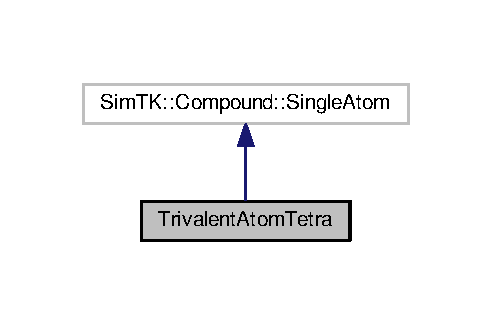
\includegraphics[width=236pt]{classTrivalentAtomTetra__inherit__graph}
\end{center}
\end{figure}


Collaboration diagram for Trivalent\+Atom\+Tetra\+:\nopagebreak
\begin{figure}[H]
\begin{center}
\leavevmode
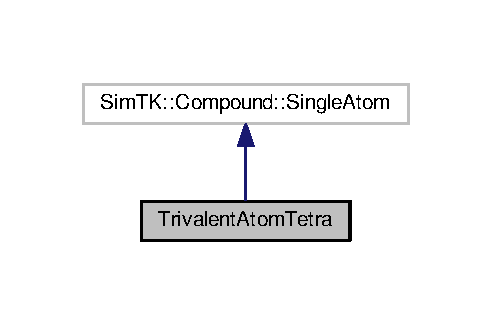
\includegraphics[width=236pt]{classTrivalentAtomTetra__coll__graph}
\end{center}
\end{figure}
\subsection*{Public Member Functions}
\begin{DoxyCompactItemize}
\item 
\hyperlink{classTrivalentAtomTetra_aceb0dcbcafa9398de59f99b30a20a63a}{Trivalent\+Atom\+Tetra} (const Sim\+T\+K\+::\+Compound\+::\+Atom\+Name \&atom\+Name, const Sim\+T\+K\+::\+Element \&element)
\end{DoxyCompactItemize}


\subsection{Detailed Description}
Trivalent Atom Class with tetrahedral geometry (ex. positive N) Bond centers are named \char`\"{}bond1\char`\"{}, \char`\"{}bond2\char`\"{}, and \char`\"{}bond3\char`\"{} 

\subsection{Constructor \& Destructor Documentation}
\index{Trivalent\+Atom\+Tetra@{Trivalent\+Atom\+Tetra}!Trivalent\+Atom\+Tetra@{Trivalent\+Atom\+Tetra}}
\index{Trivalent\+Atom\+Tetra@{Trivalent\+Atom\+Tetra}!Trivalent\+Atom\+Tetra@{Trivalent\+Atom\+Tetra}}
\subsubsection[{\texorpdfstring{Trivalent\+Atom\+Tetra(const Sim\+T\+K\+::\+Compound\+::\+Atom\+Name \&atom\+Name, const Sim\+T\+K\+::\+Element \&element)}{TrivalentAtomTetra(const SimTK::Compound::AtomName &atomName, const SimTK::Element &element)}}]{\setlength{\rightskip}{0pt plus 5cm}Trivalent\+Atom\+Tetra\+::\+Trivalent\+Atom\+Tetra (
\begin{DoxyParamCaption}
\item[{const Sim\+T\+K\+::\+Compound\+::\+Atom\+Name \&}]{atom\+Name, }
\item[{const Sim\+T\+K\+::\+Element \&}]{element}
\end{DoxyParamCaption}
)}\hypertarget{classTrivalentAtomTetra_aceb0dcbcafa9398de59f99b30a20a63a}{}\label{classTrivalentAtomTetra_aceb0dcbcafa9398de59f99b30a20a63a}

\begin{DoxyParams}{Parameters}
{\em atom\+Name} & name for new atom \\
\hline
{\em element} & element for new atom \\
\hline
\end{DoxyParams}


The documentation for this class was generated from the following files\+:\begin{DoxyCompactItemize}
\item 
include/gmolmodel/\hyperlink{TrivalentAtomTetra_8hpp}{Trivalent\+Atom\+Tetra.\+hpp}\item 
src/Trivalent\+Atom\+Tetra.\+cpp\end{DoxyCompactItemize}

\hypertarget{classWorld}{}\section{World Class Reference}
\label{classWorld}\index{World@{World}}


{\ttfamily \#include $<$World.\+hpp$>$}



Collaboration diagram for World\+:\nopagebreak
\begin{figure}[H]
\begin{center}
\leavevmode
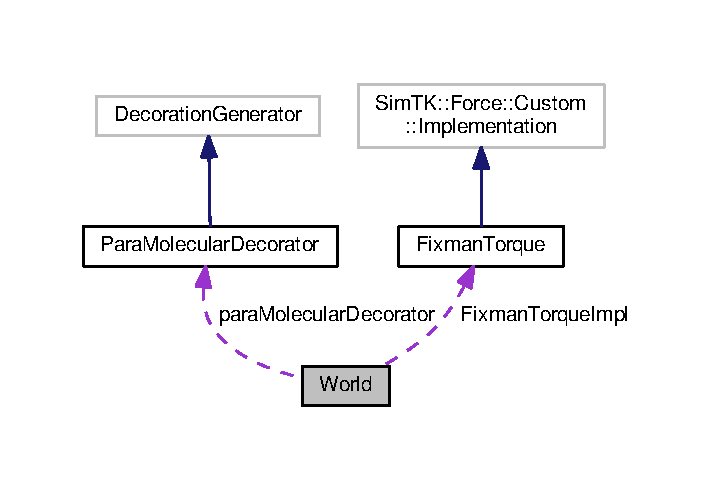
\includegraphics[width=343pt]{classWorld__coll__graph}
\end{center}
\end{figure}
\subsection*{Public Member Functions}
\begin{DoxyCompactItemize}
\item 
\hyperlink{classWorld_a5ce131833831520888e5bf6e75526438}{World} (int world\+Index, bool is\+Visual=true, Sim\+T\+K\+::\+Real visualizer\+Frequency=0.\+0015)
\item 
\hyperlink{classWorld_a8c73fba541a5817fff65147ba47cd827}{$\sim$\+World} ()
\item 
void \hyperlink{classWorld_aa71c8ba6b3fa1c580163cc144decf4a0}{Add\+Molecule} (\hyperlink{classreadAmberInput}{read\+Amber\+Input} $\ast$amber\+Reader, std\+::string rb\+FN, std\+::string flex\+FN, std\+::string regimen\+Spec, std\+::string arg\+Root)
\item 
int \hyperlink{classWorld_a321388cc18359edab1f99573188fb973}{get\+Nof\+Molecules} ()
\item 
void \hyperlink{classWorld_ab197cd25a9a29e785d329e31b6c5a2c3}{model\+Topologies} (std\+::string Ground\+To\+Compound\+Mobilizer\+Type)
\item 
const Sim\+T\+K\+::\+State \& {\bfseries realize\+Topology} (void)\hypertarget{classWorld_a7d8f9e7e5e13a7617e9b08b41b8ef608}{}\label{classWorld_a7d8f9e7e5e13a7617e9b08b41b8ef608}

\item 
void {\bfseries load\+Compound\+Related\+Maps} (void)\hypertarget{classWorld_ae71eef1e629e38141a5d75bb08372bb1}{}\label{classWorld_ae71eef1e629e38141a5d75bb08372bb1}

\item 
void {\bfseries load\+Mobods\+Related\+Maps} (void)\hypertarget{classWorld_a82fd50ef35ef6b153916102957817a3b}{}\label{classWorld_a82fd50ef35ef6b153916102957817a3b}

\item 
std\+::vector$<$ std\+::vector$<$ std\+::pair$<$ \hyperlink{classbSpecificAtom}{b\+Specific\+Atom} $\ast$, Sim\+T\+K\+::\+Vec3 $>$ $>$ $>$ \hyperlink{classWorld_a4b642cb465b7f7e144045351eef3ff60}{get\+Atoms\+Locations\+In\+Ground} (const Sim\+T\+K\+::\+State \&)
\item 
Sim\+T\+K\+::\+State \& \hyperlink{classWorld_ac7f0377e169f07e614ac664f1b0937c2}{set\+Atoms\+Locations\+In\+Ground} (Sim\+T\+K\+::\+State \&, std\+::vector$<$ std\+::vector$<$ std\+::pair$<$ \hyperlink{classbSpecificAtom}{b\+Specific\+Atom} $\ast$, Sim\+T\+K\+::\+Vec3 $>$ $>$ $>$ other\+Worlds\+Atoms\+Locations)
\item 
Compound\+System $\ast$ \hyperlink{classWorld_a94e5791e5b951a2087bbf995bf4aeff9}{get\+Compound\+System} () const 
\item 
void \hyperlink{classWorld_af4eaaaf451cd2cdceb490012fd7886b4}{set\+Compound\+System} (Compound\+System $\ast$\hyperlink{classWorld_a63269bd638b21445a78de794c97ee592}{compound\+System})
\item 
void \hyperlink{classWorld_a6e702362f7fd93376e76fc07256bdac7}{update\+Atom\+Lists\+From\+Compound} (const Sim\+T\+K\+::\+State \&state)
\item 
void \hyperlink{classWorld_ad3a225d5cdbb616866557a7dfa47f5a9}{update\+Coord\+Buffers} (void)
\item 
std\+::vector$<$ Sim\+T\+K\+::\+Real $>$ \hyperlink{classWorld_aa8b3082bb20557b070fad5dff6417d07}{get\+Xs} (void)
\item 
std\+::vector$<$ Sim\+T\+K\+::\+Real $>$ {\bfseries get\+Ys} (void)\hypertarget{classWorld_a6bf83fa6b3343cc65671122514671a89}{}\label{classWorld_a6bf83fa6b3343cc65671122514671a89}

\item 
std\+::vector$<$ Sim\+T\+K\+::\+Real $>$ {\bfseries get\+Zs} (void)\hypertarget{classWorld_a2969bfb385f741cd29046a310bae5df8}{}\label{classWorld_a2969bfb385f741cd29046a310bae5df8}

\item 
const \hyperlink{classTopology}{Topology} \& \hyperlink{classWorld_a32e376d68e307d97c2ecb6728b15bfc7}{get\+Topology} (int molecule\+Number) const 
\item 
\hyperlink{classTopology}{Topology} \& \hyperlink{classWorld_a18eded7d9547d0409f9595f2faafa16a}{upd\+Topology} (int molecule\+Number)
\item 
Sim\+T\+K\+::\+Real \hyperlink{classWorld_a6166532b83968e6fb2a428cecb93bc7e}{get\+Temperature} (void)
\item 
void \hyperlink{classWorld_a8fbd26bdd06cde3b45827ab06de4d792}{set\+Temperature} (Sim\+T\+K\+::\+Real)
\item 
void \hyperlink{classWorld_a2be6866ca33c4d8251d3f4421e1cd69a}{set\+Seed} (int which\+Sampler, unsigned long long int)
\item 
unsigned long long int {\bfseries get\+Seed} (int which\+Sampler)\hypertarget{classWorld_a138dca3b00502309aead4c2e1ce51703}{}\label{classWorld_a138dca3b00502309aead4c2e1ce51703}

\item 
void \hyperlink{classWorld_a8c3b18966e8f68d1f4e95f72229717bd}{add\+Fixman\+Torque} ()
\item 
void \hyperlink{classWorld_a6ec2e5a731fdedeb50066a7183d3a611}{set\+Amber\+Force\+Field\+Scale\+Factors} (void)
\item 
void \hyperlink{classWorld_ae6935057ff0b657b46e233e4af635b9f}{set\+Global\+Force\+Field\+Scale\+Factor} (Sim\+T\+K\+::\+Real)
\item 
void \hyperlink{classWorld_aa551dedf34c94145302d243b280122ab}{set\+Gbsa\+Global\+Scale\+Factor} (Sim\+T\+K\+::\+Real)
\item 
Sim\+T\+K\+::\+Du\+M\+M\+Force\+Field\+Subsystem $\ast$ \hyperlink{classWorld_a280165d3e24d0178a3fcd46864149efc}{upd\+Force\+Field} (void)
\item 
bool \hyperlink{classWorld_a4729653287f71760ba62f1a2b2ccf1a0}{is\+Using\+Fixman\+Torque} (void)
\item 
int \hyperlink{classWorld_add8943809f8160896ad33c6b33b716a1}{get\+Nof\+Samples} (void)
\item 
int \hyperlink{classWorld_ac0feb583f91eb5b844b8e4686c03d5e1}{get\+Nof\+Samplers} (void)
\item 
Base\+Sampler $\ast$ \hyperlink{classWorld_a9b96dc609f0f5200fb40ab798ae3ba63}{add\+Sampler} (std\+::string)
\item 
Base\+Sampler $\ast$ \hyperlink{classWorld_aacce8c70433c672b9f23ebb98b150ee9}{add\+Sampler} (Sampler\+Name)
\item 
const Base\+Sampler $\ast$ \hyperlink{classWorld_a53f849fe16026bbc02893dc28ae9d0e8}{get\+Sampler} (int which)
\item 
Base\+Sampler $\ast$ \hyperlink{classWorld_a3a52497539ba32fc205a94e1d3187617}{upd\+Sampler} (int which)
\item 
\hyperlink{classFixmanTorque}{Fixman\+Torque} $\ast$ \hyperlink{classWorld_a6fad7a67c4975e171e675d4fe979245b}{upd\+Fixman\+Torque} (void)
\item 
\hyperlink{classFixmanTorque}{Fixman\+Torque} $\ast$ \hyperlink{classWorld_a64203e9d832b1fdad7eb03bbed4e8f30}{get\+Fixman\+Torque} (void) const 
\item 
void \hyperlink{classWorld_aa0b30ed0088bf78621cae35160285554}{Print\+Simbody\+State\+Cache} (Sim\+T\+K\+::\+State \&)
\item 
void \hyperlink{classWorld_a3b7eebabe8824024af70a3d1175c0b97}{print\+Poss} (const Sim\+T\+K\+::\+Compound \&c, Sim\+T\+K\+::\+State \&some\+State)
\item 
void \hyperlink{classWorld_a8fd55c5c3f0e92e3af0c5658063ef470}{print\+Vels} (const Sim\+T\+K\+::\+Compound \&c, Sim\+T\+K\+::\+State \&some\+State)
\item 
void \hyperlink{classWorld_ad38f29681e5c31a523634dd23a73f075}{print\+Poss\+Vels} (const Sim\+T\+K\+::\+Compound \&c, Sim\+T\+K\+::\+State \&some\+State)
\end{DoxyCompactItemize}
\subsection*{Public Attributes}
\begin{DoxyCompactItemize}
\item 
Sim\+T\+K\+::\+Compound\+System $\ast$ \hyperlink{classWorld_a63269bd638b21445a78de794c97ee592}{compound\+System}
\item 
Sim\+T\+K\+::\+Simbody\+Matter\+Subsystem $\ast$ \hyperlink{classWorld_adc0da6db32a40c1cc09e29f7044ac3e6}{matter}
\item 
Sim\+T\+K\+::\+General\+Force\+Subsystem $\ast$ \hyperlink{classWorld_a25f41543a35f1950cde1e7a70a01d38d}{forces}
\item 
\hyperlink{classFixmanTorque}{Fixman\+Torque} $\ast$ \hyperlink{classWorld_a365134a878260d3e05efc93634b697df}{Fixman\+Torque\+Impl}
\item 
Sim\+T\+K\+::\+Force\+::\+Custom $\ast$ {\bfseries Ext\+Force}\hypertarget{classWorld_a32035c92ef74b9e8e91fedfdd152b112}{}\label{classWorld_a32035c92ef74b9e8e91fedfdd152b112}

\item 
Sim\+T\+K\+::\+Du\+M\+M\+Force\+Field\+Subsystem $\ast$ \hyperlink{classWorld_a49e379a00c0f908542349ee979775e8d}{force\+Field}
\item 
int \hyperlink{classWorld_a88ce5b19230917725b4c5656581d04e6}{molecule\+Count}
\item 
std\+::vector$<$ \hyperlink{classTopology}{Topology} $\ast$ $>$ \hyperlink{classWorld_aa0c16379fe096948946e73bd2a34bbb9}{topologies}
\item 
std\+::string {\bfseries root\+Mobility}\hypertarget{classWorld_afbe82ba1b4c10f2d034774c78fe1d36d}{}\label{classWorld_afbe82ba1b4c10f2d034774c78fe1d36d}

\item 
std\+::vector$<$ Sim\+T\+K\+::\+Real $>$ \hyperlink{classWorld_a0284a9971261c375fb04561a0f4821e6}{Xs}
\item 
std\+::vector$<$ Sim\+T\+K\+::\+Real $>$ {\bfseries Ys}\hypertarget{classWorld_afd6148945636421af67bf0967b3a1a1e}{}\label{classWorld_afd6148945636421af67bf0967b3a1a1e}

\item 
std\+::vector$<$ Sim\+T\+K\+::\+Real $>$ {\bfseries Zs}\hypertarget{classWorld_a34638c9fa524b941b8110d935ed79f32}{}\label{classWorld_a34638c9fa524b941b8110d935ed79f32}

\item 
Sim\+T\+K\+::\+Transform $\ast$ \hyperlink{classWorld_a615e5483cdea05073c6a9cde2a945433}{T\+Vector}
\item 
int $\ast$$\ast$ \hyperlink{classWorld_ae6ee20b37727cb29bbb29fa57e4b4ccc}{mbx\+Tree\+Mat}
\item 
Sim\+T\+K\+::\+Real $\ast$ {\bfseries branch\+Mass\+Vec}\hypertarget{classWorld_aa1e17875d970e2a5866dccbe92794408}{}\label{classWorld_aa1e17875d970e2a5866dccbe92794408}

\item 
Sim\+T\+K\+::\+Real {\bfseries temperature}\hypertarget{classWorld_af6e99c28c46a3028b19bdd9eddf1e32d}{}\label{classWorld_af6e99c28c46a3028b19bdd9eddf1e32d}

\item 
Sim\+T\+K\+::\+Verlet\+Integrator $\ast$ {\bfseries integ}\hypertarget{classWorld_a0c1825a5bccd943e622667d4f2361bfb}{}\label{classWorld_a0c1825a5bccd943e622667d4f2361bfb}

\item 
Sim\+T\+K\+::\+Time\+Stepper $\ast$ {\bfseries ts}\hypertarget{classWorld_adcb1faeb373c470571e2ab170f7a324a}{}\label{classWorld_adcb1faeb373c470571e2ab170f7a324a}

\item 
std\+::vector$<$ Base\+Sampler $\ast$ $>$ {\bfseries samplers}\hypertarget{classWorld_a138dac67fc55edc3464cea3ce7efb927}{}\label{classWorld_a138dac67fc55edc3464cea3ce7efb927}

\item 
bool {\bfseries \+\_\+use\+Fixman\+Torque}\hypertarget{classWorld_a5820bfb2de987a51015b86900d55c076}{}\label{classWorld_a5820bfb2de987a51015b86900d55c076}

\item 
int {\bfseries nof\+Samples}\hypertarget{classWorld_a94879de144abf83cc275d9306eeab37f}{}\label{classWorld_a94879de144abf83cc275d9306eeab37f}

\item 
bool {\bfseries visual}\hypertarget{classWorld_a204e8ead4fb79fdbfd6b5b7738eca7d9}{}\label{classWorld_a204e8ead4fb79fdbfd6b5b7738eca7d9}

\item 
\hyperlink{classParaMolecularDecorator}{Para\+Molecular\+Decorator} $\ast$ {\bfseries para\+Molecular\+Decorator} = nullptr\hypertarget{classWorld_aa1960e6a68168fbdac28cbda7f2dbba8}{}\label{classWorld_aa1960e6a68168fbdac28cbda7f2dbba8}

\item 
Sim\+T\+K\+::\+Decoration\+Subsystem $\ast$ {\bfseries decorations}\hypertarget{classWorld_abf703a0e3e84b43b0b33dcd2de3fa2ea}{}\label{classWorld_abf703a0e3e84b43b0b33dcd2de3fa2ea}

\item 
Sim\+T\+K\+::\+Visualizer $\ast$ {\bfseries visualizer}\hypertarget{classWorld_a2174a847c16ebce5fd6aa9cca5ef4075}{}\label{classWorld_a2174a847c16ebce5fd6aa9cca5ef4075}

\item 
Sim\+T\+K\+::\+Visualizer\+::\+Reporter $\ast$ {\bfseries visualizer\+Reporter}\hypertarget{classWorld_a8fe1c13cc40f1d32ecfb97fbacf01a31}{}\label{classWorld_a8fe1c13cc40f1d32ecfb97fbacf01a31}

\item 
int {\bfseries own\+World\+Index}\hypertarget{classWorld_a01aa97e5cd329fe3b4f5cefd86ecdc07}{}\label{classWorld_a01aa97e5cd329fe3b4f5cefd86ecdc07}

\end{DoxyCompactItemize}


\subsection{Detailed Description}
Contains a Symbody system and additional data that define a regimen 

\subsection{Constructor \& Destructor Documentation}
\index{World@{World}!World@{World}}
\index{World@{World}!World@{World}}
\subsubsection[{\texorpdfstring{World(int world\+Index, bool is\+Visual=true, Sim\+T\+K\+::\+Real visualizer\+Frequency=0.\+0015)}{World(int worldIndex, bool isVisual=true, SimTK::Real visualizerFrequency=0.0015)}}]{\setlength{\rightskip}{0pt plus 5cm}World\+::\+World (
\begin{DoxyParamCaption}
\item[{int}]{world\+Index, }
\item[{bool}]{is\+Visual = {\ttfamily true}, }
\item[{Sim\+T\+K\+::\+Real}]{visualizer\+Frequency = {\ttfamily 0.0015}}
\end{DoxyParamCaption}
)}\hypertarget{classWorld_a5ce131833831520888e5bf6e75526438}{}\label{classWorld_a5ce131833831520888e5bf6e75526438}
Constructor

Constructor. Initializes the following pretty much empty objects\+:
\begin{DoxyItemize}
\item Compound\+System,
\begin{DoxyItemize}
\item Simbody\+Matter\+Subsystem, General\+Force\+Subsystem, Decoration\+Subsystem, Visualizer, Visualizer\+::\+Reporter, Du\+M\+M\+Force\+Field\+Subsystem,
\end{DoxyItemize}
\item Integrator with a Time\+Stepper on top 
\end{DoxyItemize}\index{World@{World}!````~World@{$\sim$\+World}}
\index{````~World@{$\sim$\+World}!World@{World}}
\subsubsection[{\texorpdfstring{$\sim$\+World()}{~World()}}]{\setlength{\rightskip}{0pt plus 5cm}World\+::$\sim$\+World (
\begin{DoxyParamCaption}
{}
\end{DoxyParamCaption}
)}\hypertarget{classWorld_a8c73fba541a5817fff65147ba47cd827}{}\label{classWorld_a8c73fba541a5817fff65147ba47cd827}
Destructor 

\subsection{Member Function Documentation}
\index{World@{World}!add\+Fixman\+Torque@{add\+Fixman\+Torque}}
\index{add\+Fixman\+Torque@{add\+Fixman\+Torque}!World@{World}}
\subsubsection[{\texorpdfstring{add\+Fixman\+Torque()}{addFixmanTorque()}}]{\setlength{\rightskip}{0pt plus 5cm}void World\+::add\+Fixman\+Torque (
\begin{DoxyParamCaption}
{}
\end{DoxyParamCaption}
)}\hypertarget{classWorld_a8c3b18966e8f68d1f4e95f72229717bd}{}\label{classWorld_a8c3b18966e8f68d1f4e95f72229717bd}
Use the Fixman torque as an additional force subsystem. Careful not have different temperatures for \hyperlink{classWorld}{World} and Fixman Torque.

Set up Fixman torque \index{World@{World}!Add\+Molecule@{Add\+Molecule}}
\index{Add\+Molecule@{Add\+Molecule}!World@{World}}
\subsubsection[{\texorpdfstring{Add\+Molecule(read\+Amber\+Input $\ast$amber\+Reader, std\+::string rb\+F\+N, std\+::string flex\+F\+N, std\+::string regimen\+Spec, std\+::string arg\+Root)}{AddMolecule(readAmberInput *amberReader, std::string rbFN, std::string flexFN, std::string regimenSpec, std::string argRoot)}}]{\setlength{\rightskip}{0pt plus 5cm}void World\+::\+Add\+Molecule (
\begin{DoxyParamCaption}
\item[{{\bf read\+Amber\+Input} $\ast$}]{amber\+Reader, }
\item[{std\+::string}]{rb\+FN, }
\item[{std\+::string}]{flex\+FN, }
\item[{std\+::string}]{regimen\+Spec, }
\item[{std\+::string}]{arg\+Root}
\end{DoxyParamCaption}
)}\hypertarget{classWorld_aa71c8ba6b3fa1c580163cc144decf4a0}{}\label{classWorld_aa71c8ba6b3fa1c580163cc144decf4a0}
Creates a topology object and based on amber\+Reader forcefield parameters -\/ defines Biotypes; -\/ adds B\+AT parameters to Du\+MM

Creates Gmolmodel topologies objects and based on amber\+Reader forcefield adds parameters\+: defines Biotypes; -\/ adds B\+AT parameters to Du\+MM. Also creates decorations for visualizers \index{World@{World}!add\+Sampler@{add\+Sampler}}
\index{add\+Sampler@{add\+Sampler}!World@{World}}
\subsubsection[{\texorpdfstring{add\+Sampler(std\+::string)}{addSampler(std::string)}}]{\setlength{\rightskip}{0pt plus 5cm}Base\+Sampler$\ast$ World\+::add\+Sampler (
\begin{DoxyParamCaption}
\item[{std\+::string}]{}
\end{DoxyParamCaption}
)}\hypertarget{classWorld_a9b96dc609f0f5200fb40ab798ae3ba63}{}\label{classWorld_a9b96dc609f0f5200fb40ab798ae3ba63}
Add a sampler to the \hyperlink{classWorld}{World} \index{World@{World}!add\+Sampler@{add\+Sampler}}
\index{add\+Sampler@{add\+Sampler}!World@{World}}
\subsubsection[{\texorpdfstring{add\+Sampler(\+Sampler\+Name)}{addSampler(SamplerName)}}]{\setlength{\rightskip}{0pt plus 5cm}Base\+Sampler $\ast$ World\+::add\+Sampler (
\begin{DoxyParamCaption}
\item[{Sampler\+Name}]{sampler\+Name}
\end{DoxyParamCaption}
)}\hypertarget{classWorld_aacce8c70433c672b9f23ebb98b150ee9}{}\label{classWorld_aacce8c70433c672b9f23ebb98b150ee9}
Add a sampler to this \hyperlink{classWorld}{World} using the specialized struct for samplers names. \index{World@{World}!get\+Atoms\+Locations\+In\+Ground@{get\+Atoms\+Locations\+In\+Ground}}
\index{get\+Atoms\+Locations\+In\+Ground@{get\+Atoms\+Locations\+In\+Ground}!World@{World}}
\subsubsection[{\texorpdfstring{get\+Atoms\+Locations\+In\+Ground(const Sim\+T\+K\+::\+State \&)}{getAtomsLocationsInGround(const SimTK::State &)}}]{\setlength{\rightskip}{0pt plus 5cm}std\+::vector$<$ std\+::vector$<$ std\+::pair$<$ {\bf b\+Specific\+Atom} $\ast$, Sim\+T\+K\+::\+Vec3 $>$ $>$ $>$ World\+::get\+Atoms\+Locations\+In\+Ground (
\begin{DoxyParamCaption}
\item[{const Sim\+T\+K\+::\+State \&}]{state}
\end{DoxyParamCaption}
)}\hypertarget{classWorld_a4b642cb465b7f7e144045351eef3ff60}{}\label{classWorld_a4b642cb465b7f7e144045351eef3ff60}
Get the current Compound Cartesian coords

Return a 2D vector representing all the coordinates of this \hyperlink{classWorld}{World}. The first dimension represents the molecules (topologies) and the second dimension (inner) represents the coordinates. The second inner dimension type is pair of b\+Specific\+Atom$\ast$ and a Vec3. Thus, besides coordinates, it contains all the information in \hyperlink{classbSpecificAtom}{b\+Specific\+Atom} as well. The bottleneck here is the calc\+Atom\+Location\+In\+Ground\+Frame from Compound. \index{World@{World}!get\+Compound\+System@{get\+Compound\+System}}
\index{get\+Compound\+System@{get\+Compound\+System}!World@{World}}
\subsubsection[{\texorpdfstring{get\+Compound\+System() const }{getCompoundSystem() const }}]{\setlength{\rightskip}{0pt plus 5cm}Compound\+System $\ast$ World\+::get\+Compound\+System (
\begin{DoxyParamCaption}
{}
\end{DoxyParamCaption}
) const}\hypertarget{classWorld_a94e5791e5b951a2087bbf995bf4aeff9}{}\label{classWorld_a94e5791e5b951a2087bbf995bf4aeff9}
Return own Compound\+System \index{World@{World}!get\+Fixman\+Torque@{get\+Fixman\+Torque}}
\index{get\+Fixman\+Torque@{get\+Fixman\+Torque}!World@{World}}
\subsubsection[{\texorpdfstring{get\+Fixman\+Torque(void) const }{getFixmanTorque(void) const }}]{\setlength{\rightskip}{0pt plus 5cm}{\bf Fixman\+Torque} $\ast$ World\+::get\+Fixman\+Torque (
\begin{DoxyParamCaption}
\item[{void}]{}
\end{DoxyParamCaption}
) const}\hypertarget{classWorld_a64203e9d832b1fdad7eb03bbed4e8f30}{}\label{classWorld_a64203e9d832b1fdad7eb03bbed4e8f30}
Get pointer to \hyperlink{classFixmanTorque}{Fixman\+Torque} implementation \index{World@{World}!get\+Nof\+Molecules@{get\+Nof\+Molecules}}
\index{get\+Nof\+Molecules@{get\+Nof\+Molecules}!World@{World}}
\subsubsection[{\texorpdfstring{get\+Nof\+Molecules()}{getNofMolecules()}}]{\setlength{\rightskip}{0pt plus 5cm}int World\+::get\+Nof\+Molecules (
\begin{DoxyParamCaption}
\item[{void}]{}
\end{DoxyParamCaption}
)}\hypertarget{classWorld_a321388cc18359edab1f99573188fb973}{}\label{classWorld_a321388cc18359edab1f99573188fb973}
Get the number of molecules \index{World@{World}!get\+Nof\+Samplers@{get\+Nof\+Samplers}}
\index{get\+Nof\+Samplers@{get\+Nof\+Samplers}!World@{World}}
\subsubsection[{\texorpdfstring{get\+Nof\+Samplers(void)}{getNofSamplers(void)}}]{\setlength{\rightskip}{0pt plus 5cm}int World\+::get\+Nof\+Samplers (
\begin{DoxyParamCaption}
\item[{void}]{}
\end{DoxyParamCaption}
)}\hypertarget{classWorld_ac0feb583f91eb5b844b8e4686c03d5e1}{}\label{classWorld_ac0feb583f91eb5b844b8e4686c03d5e1}
\hyperlink{classSampler}{Sampler} manipulation functions

How many Samplers does this \hyperlink{classWorld}{World} have. \index{World@{World}!get\+Nof\+Samples@{get\+Nof\+Samples}}
\index{get\+Nof\+Samples@{get\+Nof\+Samples}!World@{World}}
\subsubsection[{\texorpdfstring{get\+Nof\+Samples(void)}{getNofSamples(void)}}]{\setlength{\rightskip}{0pt plus 5cm}int World\+::get\+Nof\+Samples (
\begin{DoxyParamCaption}
\item[{void}]{}
\end{DoxyParamCaption}
)}\hypertarget{classWorld_add8943809f8160896ad33c6b33b716a1}{}\label{classWorld_add8943809f8160896ad33c6b33b716a1}
How many samples did we have so far

How many samples do we have so far \index{World@{World}!get\+Sampler@{get\+Sampler}}
\index{get\+Sampler@{get\+Sampler}!World@{World}}
\subsubsection[{\texorpdfstring{get\+Sampler(int which)}{getSampler(int which)}}]{\setlength{\rightskip}{0pt plus 5cm}const Base\+Sampler $\ast$ World\+::get\+Sampler (
\begin{DoxyParamCaption}
\item[{int}]{which}
\end{DoxyParamCaption}
)}\hypertarget{classWorld_a53f849fe16026bbc02893dc28ae9d0e8}{}\label{classWorld_a53f849fe16026bbc02893dc28ae9d0e8}
Get a sampler based on its position in the samplers vector \index{World@{World}!get\+Temperature@{get\+Temperature}}
\index{get\+Temperature@{get\+Temperature}!World@{World}}
\subsubsection[{\texorpdfstring{get\+Temperature(void)}{getTemperature(void)}}]{\setlength{\rightskip}{0pt plus 5cm}Sim\+T\+K\+::\+Real World\+::get\+Temperature (
\begin{DoxyParamCaption}
\item[{void}]{}
\end{DoxyParamCaption}
)}\hypertarget{classWorld_a6166532b83968e6fb2a428cecb93bc7e}{}\label{classWorld_a6166532b83968e6fb2a428cecb93bc7e}
Get the \hyperlink{classWorld}{World} (macro) temperature

Get the \hyperlink{classWorld}{World} temperature \index{World@{World}!get\+Topology@{get\+Topology}}
\index{get\+Topology@{get\+Topology}!World@{World}}
\subsubsection[{\texorpdfstring{get\+Topology(int molecule\+Number) const }{getTopology(int moleculeNumber) const }}]{\setlength{\rightskip}{0pt plus 5cm}const {\bf Topology} \& World\+::get\+Topology (
\begin{DoxyParamCaption}
\item[{int}]{molecule\+Number}
\end{DoxyParamCaption}
) const}\hypertarget{classWorld_a32e376d68e307d97c2ecb6728b15bfc7}{}\label{classWorld_a32e376d68e307d97c2ecb6728b15bfc7}
Access to molecule (\hyperlink{classTopology}{Topology}) objects Get a readble reference of one of the molecules

Get a const reference to a molecule \index{World@{World}!get\+Xs@{get\+Xs}}
\index{get\+Xs@{get\+Xs}!World@{World}}
\subsubsection[{\texorpdfstring{get\+Xs(void)}{getXs(void)}}]{\setlength{\rightskip}{0pt plus 5cm}std\+::vector$<$ Sim\+T\+K\+::\+Real $>$ World\+::get\+Xs (
\begin{DoxyParamCaption}
\item[{void}]{}
\end{DoxyParamCaption}
)}\hypertarget{classWorld_aa8b3082bb20557b070fad5dff6417d07}{}\label{classWorld_aa8b3082bb20557b070fad5dff6417d07}
Get the coordinates buffers

Get the coordinates from buffers \index{World@{World}!is\+Using\+Fixman\+Torque@{is\+Using\+Fixman\+Torque}}
\index{is\+Using\+Fixman\+Torque@{is\+Using\+Fixman\+Torque}!World@{World}}
\subsubsection[{\texorpdfstring{is\+Using\+Fixman\+Torque(void)}{isUsingFixmanTorque(void)}}]{\setlength{\rightskip}{0pt plus 5cm}bool World\+::is\+Using\+Fixman\+Torque (
\begin{DoxyParamCaption}
\item[{void}]{}
\end{DoxyParamCaption}
)}\hypertarget{classWorld_a4729653287f71760ba62f1a2b2ccf1a0}{}\label{classWorld_a4729653287f71760ba62f1a2b2ccf1a0}
Return true if the Fixman torque flag is set

Check if the Fixman torque flag is set \index{World@{World}!model\+Topologies@{model\+Topologies}}
\index{model\+Topologies@{model\+Topologies}!World@{World}}
\subsubsection[{\texorpdfstring{model\+Topologies(std\+::string Ground\+To\+Compound\+Mobilizer\+Type)}{modelTopologies(std::string GroundToCompoundMobilizerType)}}]{\setlength{\rightskip}{0pt plus 5cm}void World\+::model\+Topologies (
\begin{DoxyParamCaption}
\item[{std\+::string}]{Ground\+To\+Compound\+Mobilizer\+Type}
\end{DoxyParamCaption}
)}\hypertarget{classWorld_ab197cd25a9a29e785d329e31b6c5a2c3}{}\label{classWorld_ab197cd25a9a29e785d329e31b6c5a2c3}
Calls Compound\+System.\+model\+Compounds and realizes \hyperlink{classTopology}{Topology} To be called after loading all Compounds.

Calls Compound\+System.\+model\+One\+Compound which links the Compounds to the Simbody subsystems and realizes \hyperlink{classTopology}{Topology}. To be called after setting all Compounds properties. \index{World@{World}!print\+Poss@{print\+Poss}}
\index{print\+Poss@{print\+Poss}!World@{World}}
\subsubsection[{\texorpdfstring{print\+Poss(const Sim\+T\+K\+::\+Compound \&c, Sim\+T\+K\+::\+State \&some\+State)}{printPoss(const SimTK::Compound &c, SimTK::State &someState)}}]{\setlength{\rightskip}{0pt plus 5cm}void World\+::print\+Poss (
\begin{DoxyParamCaption}
\item[{const Sim\+T\+K\+::\+Compound \&}]{c, }
\item[{Sim\+T\+K\+::\+State \&}]{advanced}
\end{DoxyParamCaption}
)}\hypertarget{classWorld_a3b7eebabe8824024af70a3d1175c0b97}{}\label{classWorld_a3b7eebabe8824024af70a3d1175c0b97}
Print a Compound Cartesian coordinates as given by Compound\+::calc\+Atom\+Location\+In\+Ground\+Frame \index{World@{World}!print\+Poss\+Vels@{print\+Poss\+Vels}}
\index{print\+Poss\+Vels@{print\+Poss\+Vels}!World@{World}}
\subsubsection[{\texorpdfstring{print\+Poss\+Vels(const Sim\+T\+K\+::\+Compound \&c, Sim\+T\+K\+::\+State \&some\+State)}{printPossVels(const SimTK::Compound &c, SimTK::State &someState)}}]{\setlength{\rightskip}{0pt plus 5cm}void World\+::print\+Poss\+Vels (
\begin{DoxyParamCaption}
\item[{const Sim\+T\+K\+::\+Compound \&}]{c, }
\item[{Sim\+T\+K\+::\+State \&}]{some\+State}
\end{DoxyParamCaption}
)}\hypertarget{classWorld_ad38f29681e5c31a523634dd23a73f075}{}\label{classWorld_ad38f29681e5c31a523634dd23a73f075}
Print a Compound Cartesian coordinates and velocities as given by Compound\+::calc\+Atom\+Location\+In\+Ground\+Frame and Compound\+::calc\+Atom\+Velocity\+In\+Ground\+Frame \index{World@{World}!Print\+Simbody\+State\+Cache@{Print\+Simbody\+State\+Cache}}
\index{Print\+Simbody\+State\+Cache@{Print\+Simbody\+State\+Cache}!World@{World}}
\subsubsection[{\texorpdfstring{Print\+Simbody\+State\+Cache(\+Sim\+T\+K\+::\+State \&)}{PrintSimbodyStateCache(SimTK::State &)}}]{\setlength{\rightskip}{0pt plus 5cm}void World\+::\+Print\+Simbody\+State\+Cache (
\begin{DoxyParamCaption}
\item[{Sim\+T\+K\+::\+State \&}]{some\+State}
\end{DoxyParamCaption}
)}\hypertarget{classWorld_aa0b30ed0088bf78621cae35160285554}{}\label{classWorld_aa0b30ed0088bf78621cae35160285554}
Print information about Simbody systems

Print information about Simbody systems. For debugging purpose. \index{World@{World}!print\+Vels@{print\+Vels}}
\index{print\+Vels@{print\+Vels}!World@{World}}
\subsubsection[{\texorpdfstring{print\+Vels(const Sim\+T\+K\+::\+Compound \&c, Sim\+T\+K\+::\+State \&some\+State)}{printVels(const SimTK::Compound &c, SimTK::State &someState)}}]{\setlength{\rightskip}{0pt plus 5cm}void World\+::print\+Vels (
\begin{DoxyParamCaption}
\item[{const Sim\+T\+K\+::\+Compound \&}]{c, }
\item[{Sim\+T\+K\+::\+State \&}]{some\+State}
\end{DoxyParamCaption}
)}\hypertarget{classWorld_a8fd55c5c3f0e92e3af0c5658063ef470}{}\label{classWorld_a8fd55c5c3f0e92e3af0c5658063ef470}
Print a Compound Cartesian velocities as given by Compound\+::calc\+Atom\+Velocity\+In\+Ground\+Frame \index{World@{World}!set\+Amber\+Force\+Field\+Scale\+Factors@{set\+Amber\+Force\+Field\+Scale\+Factors}}
\index{set\+Amber\+Force\+Field\+Scale\+Factors@{set\+Amber\+Force\+Field\+Scale\+Factors}!World@{World}}
\subsubsection[{\texorpdfstring{set\+Amber\+Force\+Field\+Scale\+Factors(void)}{setAmberForceFieldScaleFactors(void)}}]{\setlength{\rightskip}{0pt plus 5cm}void World\+::set\+Amber\+Force\+Field\+Scale\+Factors (
\begin{DoxyParamCaption}
\item[{void}]{}
\end{DoxyParamCaption}
)}\hypertarget{classWorld_a6ec2e5a731fdedeb50066a7183d3a611}{}\label{classWorld_a6ec2e5a731fdedeb50066a7183d3a611}
Amber like scale factors. \index{World@{World}!set\+Atoms\+Locations\+In\+Ground@{set\+Atoms\+Locations\+In\+Ground}}
\index{set\+Atoms\+Locations\+In\+Ground@{set\+Atoms\+Locations\+In\+Ground}!World@{World}}
\subsubsection[{\texorpdfstring{set\+Atoms\+Locations\+In\+Ground(\+Sim\+T\+K\+::\+State \&, std\+::vector$<$ std\+::vector$<$ std\+::pair$<$ b\+Specific\+Atom $\ast$, Sim\+T\+K\+::\+Vec3 $>$ $>$ $>$ other\+Worlds\+Atoms\+Locations)}{setAtomsLocationsInGround(SimTK::State &, std::vector< std::vector< std::pair< bSpecificAtom *, SimTK::Vec3 > > > otherWorldsAtomsLocations)}}]{\setlength{\rightskip}{0pt plus 5cm}Sim\+T\+K\+::\+State \& World\+::set\+Atoms\+Locations\+In\+Ground (
\begin{DoxyParamCaption}
\item[{Sim\+T\+K\+::\+State \&}]{some\+State, }
\item[{std\+::vector$<$ std\+::vector$<$ std\+::pair$<$ {\bf b\+Specific\+Atom} $\ast$, Sim\+T\+K\+::\+Vec3 $>$ $>$ $>$}]{other\+Worlds\+Atoms\+Locations}
\end{DoxyParamCaption}
)}\hypertarget{classWorld_ac7f0377e169f07e614ac664f1b0937c2}{}\label{classWorld_ac7f0377e169f07e614ac664f1b0937c2}
Set Compound, Multibody\+System and Du\+MM configurations according to some other \hyperlink{classWorld}{World}\textquotesingle{}s atoms

Set Compound, Multibody\+System and Du\+MM configurations according to some other \hyperlink{classWorld}{World}\textquotesingle{}s atoms. A body is composed of a root atom and other periferic atoms which have their own stations. Unles is a fully flexible Cartesian world, the function has the following steps\+:
\begin{DoxyEnumerate}
\item Set Compound
\item Set Du\+MM
\item Set Simbody bodies 3.\+1. Transforms X\+\_\+\+PF and X\+\_\+\+BM 3.\+2. Mass properties 
\end{DoxyEnumerate}\index{World@{World}!set\+Compound\+System@{set\+Compound\+System}}
\index{set\+Compound\+System@{set\+Compound\+System}!World@{World}}
\subsubsection[{\texorpdfstring{set\+Compound\+System(\+Compound\+System $\ast$compound\+System)}{setCompoundSystem(CompoundSystem *compoundSystem)}}]{\setlength{\rightskip}{0pt plus 5cm}void World\+::set\+Compound\+System (
\begin{DoxyParamCaption}
\item[{Compound\+System $\ast$}]{compound\+System}
\end{DoxyParamCaption}
)}\hypertarget{classWorld_af4eaaaf451cd2cdceb490012fd7886b4}{}\label{classWorld_af4eaaaf451cd2cdceb490012fd7886b4}
Set own Compound system \index{World@{World}!set\+Gbsa\+Global\+Scale\+Factor@{set\+Gbsa\+Global\+Scale\+Factor}}
\index{set\+Gbsa\+Global\+Scale\+Factor@{set\+Gbsa\+Global\+Scale\+Factor}!World@{World}}
\subsubsection[{\texorpdfstring{set\+Gbsa\+Global\+Scale\+Factor(\+Sim\+T\+K\+::\+Real)}{setGbsaGlobalScaleFactor(SimTK::Real)}}]{\setlength{\rightskip}{0pt plus 5cm}void World\+::set\+Gbsa\+Global\+Scale\+Factor (
\begin{DoxyParamCaption}
\item[{Sim\+T\+K\+::\+Real}]{scale\+Factor}
\end{DoxyParamCaption}
)}\hypertarget{classWorld_aa551dedf34c94145302d243b280122ab}{}\label{classWorld_aa551dedf34c94145302d243b280122ab}
Set G\+B\+SA implicit solvent scale factor

Set G\+B\+SA implicit solvent scale factor. \index{World@{World}!set\+Global\+Force\+Field\+Scale\+Factor@{set\+Global\+Force\+Field\+Scale\+Factor}}
\index{set\+Global\+Force\+Field\+Scale\+Factor@{set\+Global\+Force\+Field\+Scale\+Factor}!World@{World}}
\subsubsection[{\texorpdfstring{set\+Global\+Force\+Field\+Scale\+Factor(\+Sim\+T\+K\+::\+Real)}{setGlobalForceFieldScaleFactor(SimTK::Real)}}]{\setlength{\rightskip}{0pt plus 5cm}void World\+::set\+Global\+Force\+Field\+Scale\+Factor (
\begin{DoxyParamCaption}
\item[{Sim\+T\+K\+::\+Real}]{scale\+Factor}
\end{DoxyParamCaption}
)}\hypertarget{classWorld_ae6935057ff0b657b46e233e4af635b9f}{}\label{classWorld_ae6935057ff0b657b46e233e4af635b9f}
Set a global scaling factor for all the terms the forcefield

Set a global scaling factor for all the terms in the forcefield \index{World@{World}!set\+Seed@{set\+Seed}}
\index{set\+Seed@{set\+Seed}!World@{World}}
\subsubsection[{\texorpdfstring{set\+Seed(int which\+Sampler, unsigned long long int)}{setSeed(int whichSampler, unsigned long long int)}}]{\setlength{\rightskip}{0pt plus 5cm}void World\+::set\+Seed (
\begin{DoxyParamCaption}
\item[{int}]{which\+Sampler, }
\item[{unsigned long long int}]{arg\+Seed}
\end{DoxyParamCaption}
)}\hypertarget{classWorld_a2be6866ca33c4d8251d3f4421e1cd69a}{}\label{classWorld_a2be6866ca33c4d8251d3f4421e1cd69a}
Get/\+Set seed for reproducibility. \index{World@{World}!set\+Temperature@{set\+Temperature}}
\index{set\+Temperature@{set\+Temperature}!World@{World}}
\subsubsection[{\texorpdfstring{set\+Temperature(\+Sim\+T\+K\+::\+Real)}{setTemperature(SimTK::Real)}}]{\setlength{\rightskip}{0pt plus 5cm}void World\+::set\+Temperature (
\begin{DoxyParamCaption}
\item[{Sim\+T\+K\+::\+Real}]{arg\+Temperature}
\end{DoxyParamCaption}
)}\hypertarget{classWorld_a8fbd26bdd06cde3b45827ab06de4d792}{}\label{classWorld_a8fbd26bdd06cde3b45827ab06de4d792}
Set the \hyperlink{classWorld}{World} (macro) temperature

Set this \hyperlink{classWorld}{World} temperature but also ths samplers and Fixman torque temperature. \index{World@{World}!update\+Atom\+Lists\+From\+Compound@{update\+Atom\+Lists\+From\+Compound}}
\index{update\+Atom\+Lists\+From\+Compound@{update\+Atom\+Lists\+From\+Compound}!World@{World}}
\subsubsection[{\texorpdfstring{update\+Atom\+Lists\+From\+Compound(const Sim\+T\+K\+::\+State \&state)}{updateAtomListsFromCompound(const SimTK::State &state)}}]{\setlength{\rightskip}{0pt plus 5cm}void World\+::update\+Atom\+Lists\+From\+Compound (
\begin{DoxyParamCaption}
\item[{const Sim\+T\+K\+::\+State \&}]{state}
\end{DoxyParamCaption}
)}\hypertarget{classWorld_a6e702362f7fd93376e76fc07256bdac7}{}\label{classWorld_a6e702362f7fd93376e76fc07256bdac7}
Update Gmolmodel \hyperlink{classbSpecificAtom}{b\+Specific\+Atom} Cartesian coordinates according to Molmodel Compound which in turn relizes Position and uses matter to calculate locations.

Put coordinates into b\+Atom\+Lists of Topologies. When provided with a State, calc\+Atom\+Location\+In\+Ground\+Frame realizes Position and uses matter to calculate locations \index{World@{World}!update\+Coord\+Buffers@{update\+Coord\+Buffers}}
\index{update\+Coord\+Buffers@{update\+Coord\+Buffers}!World@{World}}
\subsubsection[{\texorpdfstring{update\+Coord\+Buffers(void)}{updateCoordBuffers(void)}}]{\setlength{\rightskip}{0pt plus 5cm}void World\+::update\+Coord\+Buffers (
\begin{DoxyParamCaption}
\item[{void}]{}
\end{DoxyParamCaption}
)}\hypertarget{classWorld_ad3a225d5cdbb616866557a7dfa47f5a9}{}\label{classWorld_ad3a225d5cdbb616866557a7dfa47f5a9}
To be called before use of get\+Xs, get\+Ys or get\+Zs

Fill Worlds Cartesian coordinates buffers. To be called before use of get\+Xs, get\+Ys or get\+Zs \index{World@{World}!upd\+Fixman\+Torque@{upd\+Fixman\+Torque}}
\index{upd\+Fixman\+Torque@{upd\+Fixman\+Torque}!World@{World}}
\subsubsection[{\texorpdfstring{upd\+Fixman\+Torque(void)}{updFixmanTorque(void)}}]{\setlength{\rightskip}{0pt plus 5cm}{\bf Fixman\+Torque} $\ast$ World\+::upd\+Fixman\+Torque (
\begin{DoxyParamCaption}
\item[{void}]{}
\end{DoxyParamCaption}
)}\hypertarget{classWorld_a6fad7a67c4975e171e675d4fe979245b}{}\label{classWorld_a6fad7a67c4975e171e675d4fe979245b}
Get writble pointer to \hyperlink{classFixmanTorque}{Fixman\+Torque} implementation \index{World@{World}!upd\+Force\+Field@{upd\+Force\+Field}}
\index{upd\+Force\+Field@{upd\+Force\+Field}!World@{World}}
\subsubsection[{\texorpdfstring{upd\+Force\+Field(void)}{updForceField(void)}}]{\setlength{\rightskip}{0pt plus 5cm}Sim\+T\+K\+::\+Du\+M\+M\+Force\+Field\+Subsystem $\ast$ World\+::upd\+Force\+Field (
\begin{DoxyParamCaption}
\item[{void}]{}
\end{DoxyParamCaption}
)}\hypertarget{classWorld_a280165d3e24d0178a3fcd46864149efc}{}\label{classWorld_a280165d3e24d0178a3fcd46864149efc}
Get a writeble pointer to the Du\+MM force field \index{World@{World}!upd\+Sampler@{upd\+Sampler}}
\index{upd\+Sampler@{upd\+Sampler}!World@{World}}
\subsubsection[{\texorpdfstring{upd\+Sampler(int which)}{updSampler(int which)}}]{\setlength{\rightskip}{0pt plus 5cm}Base\+Sampler $\ast$ World\+::upd\+Sampler (
\begin{DoxyParamCaption}
\item[{int}]{which}
\end{DoxyParamCaption}
)}\hypertarget{classWorld_a3a52497539ba32fc205a94e1d3187617}{}\label{classWorld_a3a52497539ba32fc205a94e1d3187617}
Get a writable sampler based on its position in the samplers vector \index{World@{World}!upd\+Topology@{upd\+Topology}}
\index{upd\+Topology@{upd\+Topology}!World@{World}}
\subsubsection[{\texorpdfstring{upd\+Topology(int molecule\+Number)}{updTopology(int moleculeNumber)}}]{\setlength{\rightskip}{0pt plus 5cm}{\bf Topology} \& World\+::upd\+Topology (
\begin{DoxyParamCaption}
\item[{int}]{molecule\+Number}
\end{DoxyParamCaption}
)}\hypertarget{classWorld_a18eded7d9547d0409f9595f2faafa16a}{}\label{classWorld_a18eded7d9547d0409f9595f2faafa16a}
Get a writeble reference of one of the molecules

Get a writble reference to the last molecule. 

\subsection{Member Data Documentation}
\index{World@{World}!compound\+System@{compound\+System}}
\index{compound\+System@{compound\+System}!World@{World}}
\subsubsection[{\texorpdfstring{compound\+System}{compoundSystem}}]{\setlength{\rightskip}{0pt plus 5cm}Sim\+T\+K\+::\+Compound\+System$\ast$ World\+::compound\+System}\hypertarget{classWorld_a63269bd638b21445a78de794c97ee592}{}\label{classWorld_a63269bd638b21445a78de794c97ee592}
System-\/$>$Multibody\+System-\/$>$Molecular\+Mechanics\+Systems-\/$>$Compound\+System \index{World@{World}!Fixman\+Torque\+Impl@{Fixman\+Torque\+Impl}}
\index{Fixman\+Torque\+Impl@{Fixman\+Torque\+Impl}!World@{World}}
\subsubsection[{\texorpdfstring{Fixman\+Torque\+Impl}{FixmanTorqueImpl}}]{\setlength{\rightskip}{0pt plus 5cm}{\bf Fixman\+Torque}$\ast$ World\+::\+Fixman\+Torque\+Impl}\hypertarget{classWorld_a365134a878260d3e05efc93634b697df}{}\label{classWorld_a365134a878260d3e05efc93634b697df}
Get writble pointer to Fixman Torque and other forces \index{World@{World}!force\+Field@{force\+Field}}
\index{force\+Field@{force\+Field}!World@{World}}
\subsubsection[{\texorpdfstring{force\+Field}{forceField}}]{\setlength{\rightskip}{0pt plus 5cm}Sim\+T\+K\+::\+Du\+M\+M\+Force\+Field\+Subsystem$\ast$ World\+::force\+Field}\hypertarget{classWorld_a49e379a00c0f908542349ee979775e8d}{}\label{classWorld_a49e379a00c0f908542349ee979775e8d}
Subsystem-\/$>$Force\+Subsystem-\/$>$Du\+M\+M\+Force\+Field\+Subsystem \index{World@{World}!forces@{forces}}
\index{forces@{forces}!World@{World}}
\subsubsection[{\texorpdfstring{forces}{forces}}]{\setlength{\rightskip}{0pt plus 5cm}Sim\+T\+K\+::\+General\+Force\+Subsystem$\ast$ World\+::forces}\hypertarget{classWorld_a25f41543a35f1950cde1e7a70a01d38d}{}\label{classWorld_a25f41543a35f1950cde1e7a70a01d38d}
Subsystem-\/$>$Force\+Subsystem-\/$>$General\+Force\+Subsystem \index{World@{World}!matter@{matter}}
\index{matter@{matter}!World@{World}}
\subsubsection[{\texorpdfstring{matter}{matter}}]{\setlength{\rightskip}{0pt plus 5cm}Sim\+T\+K\+::\+Simbody\+Matter\+Subsystem$\ast$ World\+::matter}\hypertarget{classWorld_adc0da6db32a40c1cc09e29f7044ac3e6}{}\label{classWorld_adc0da6db32a40c1cc09e29f7044ac3e6}
Subsystem-\/$>$Simbody\+Matter\+Subsystem \index{World@{World}!mbx\+Tree\+Mat@{mbx\+Tree\+Mat}}
\index{mbx\+Tree\+Mat@{mbx\+Tree\+Mat}!World@{World}}
\subsubsection[{\texorpdfstring{mbx\+Tree\+Mat}{mbxTreeMat}}]{\setlength{\rightskip}{0pt plus 5cm}int$\ast$$\ast$ World\+::mbx\+Tree\+Mat}\hypertarget{classWorld_ae6ee20b37727cb29bbb29fa57e4b4ccc}{}\label{classWorld_ae6ee20b37727cb29bbb29fa57e4b4ccc}
Topologies graphs as tables -\/ to be removed \index{World@{World}!molecule\+Count@{molecule\+Count}}
\index{molecule\+Count@{molecule\+Count}!World@{World}}
\subsubsection[{\texorpdfstring{molecule\+Count}{moleculeCount}}]{\setlength{\rightskip}{0pt plus 5cm}int World\+::molecule\+Count}\hypertarget{classWorld_a88ce5b19230917725b4c5656581d04e6}{}\label{classWorld_a88ce5b19230917725b4c5656581d04e6}
Nof molecules \index{World@{World}!topologies@{topologies}}
\index{topologies@{topologies}!World@{World}}
\subsubsection[{\texorpdfstring{topologies}{topologies}}]{\setlength{\rightskip}{0pt plus 5cm}std\+::vector$<${\bf Topology} $\ast$$>$ World\+::topologies}\hypertarget{classWorld_aa0c16379fe096948946e73bd2a34bbb9}{}\label{classWorld_aa0c16379fe096948946e73bd2a34bbb9}
Molecules (topologies$<$-\/\+Compounds) objects \index{World@{World}!T\+Vector@{T\+Vector}}
\index{T\+Vector@{T\+Vector}!World@{World}}
\subsubsection[{\texorpdfstring{T\+Vector}{TVector}}]{\setlength{\rightskip}{0pt plus 5cm}Sim\+T\+K\+::\+Transform$\ast$ World\+::\+T\+Vector}\hypertarget{classWorld_a615e5483cdea05073c6a9cde2a945433}{}\label{classWorld_a615e5483cdea05073c6a9cde2a945433}
This vector stores a configuration if is needed for later use \index{World@{World}!Xs@{Xs}}
\index{Xs@{Xs}!World@{World}}
\subsubsection[{\texorpdfstring{Xs}{Xs}}]{\setlength{\rightskip}{0pt plus 5cm}std\+::vector$<$Sim\+T\+K\+::\+Real$>$ World\+::\+Xs}\hypertarget{classWorld_a0284a9971261c375fb04561a0f4821e6}{}\label{classWorld_a0284a9971261c375fb04561a0f4821e6}
Joint types Vectors of Cartesian coordinates 

The documentation for this class was generated from the following files\+:\begin{DoxyCompactItemize}
\item 
include/gmolmodel/World.\+hpp\item 
src/World.\+cpp\end{DoxyCompactItemize}

\chapter{File Documentation}
\hypertarget{bBond_8hpp}{}\section{include/gmolmodel/b\+Bond.hpp File Reference}
\label{bBond_8hpp}\index{include/gmolmodel/b\+Bond.\+hpp@{include/gmolmodel/b\+Bond.\+hpp}}
{\ttfamily \#include \char`\"{}bgeneral.\+hpp\char`\"{}}\\*
{\ttfamily \#include \char`\"{}Robo.\+hpp\char`\"{}}\\*
{\ttfamily \#include \char`\"{}Simbody.\+h\char`\"{}}\\*
{\ttfamily \#include \char`\"{}Molmodel.\+h\char`\"{}}\\*
Include dependency graph for b\+Bond.\+hpp\+:\nopagebreak
\begin{figure}[H]
\begin{center}
\leavevmode
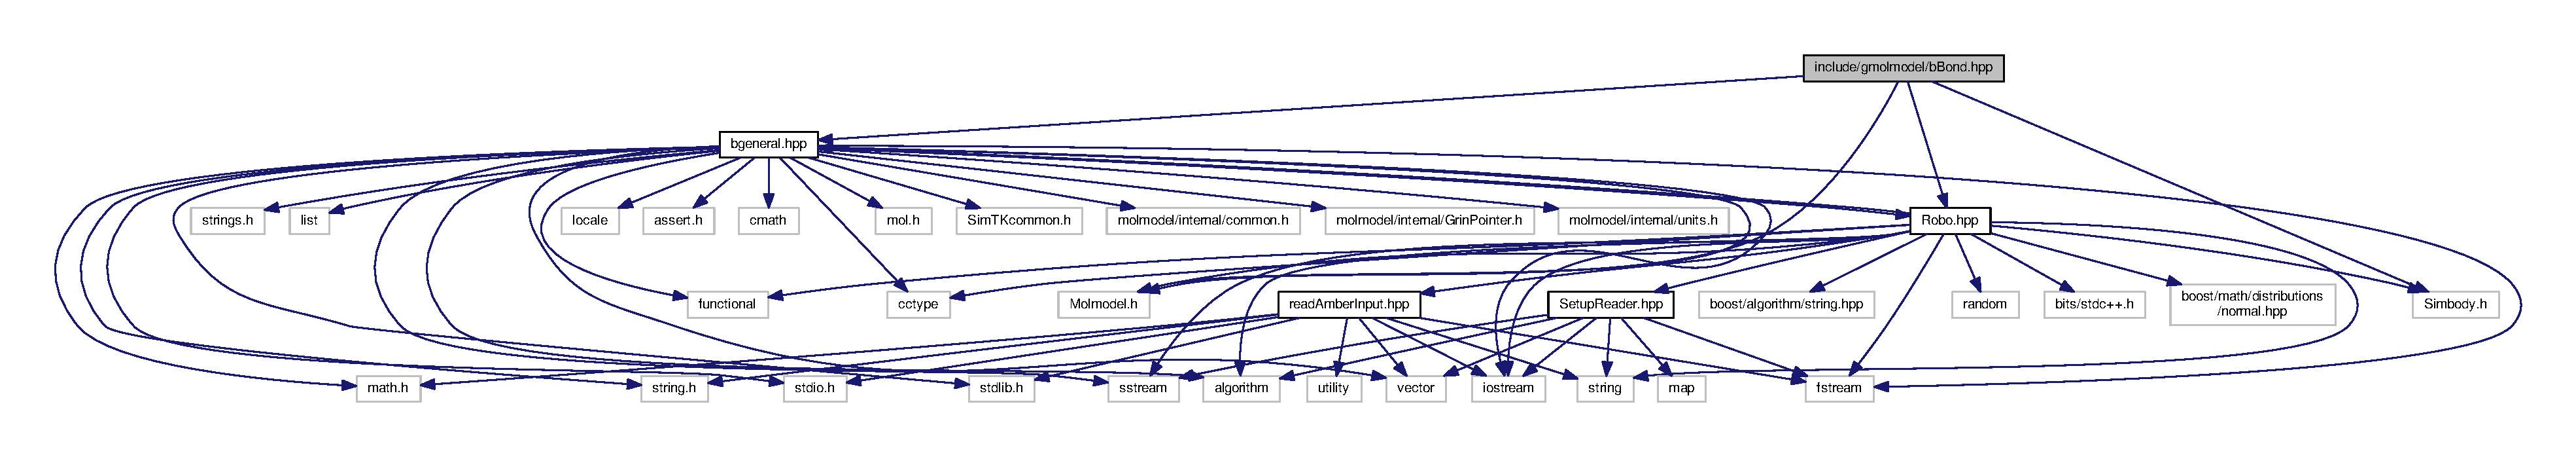
\includegraphics[width=350pt]{bBond_8hpp__incl}
\end{center}
\end{figure}
This graph shows which files directly or indirectly include this file\+:
\nopagebreak
\begin{figure}[H]
\begin{center}
\leavevmode
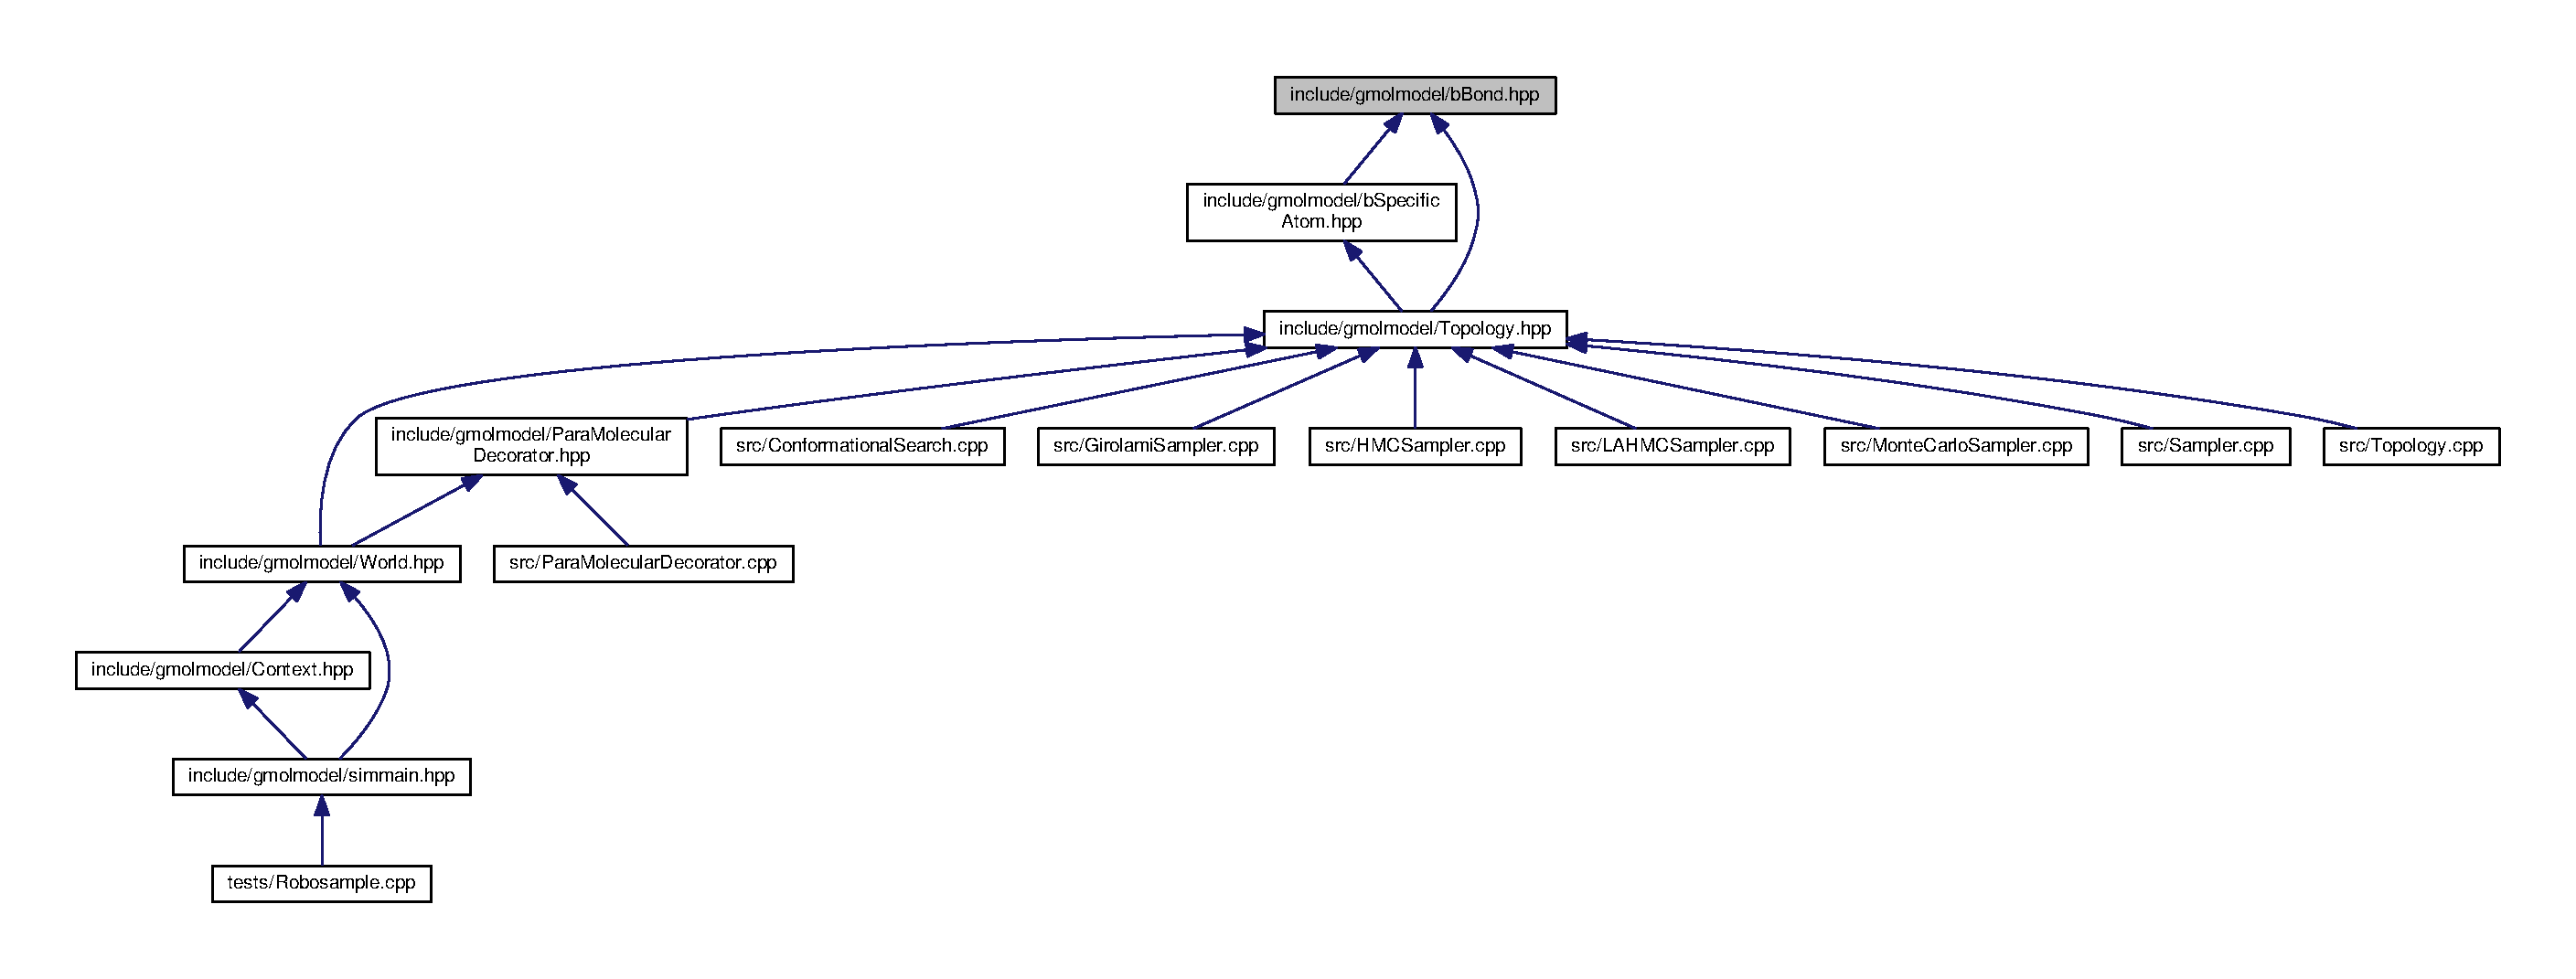
\includegraphics[width=350pt]{bBond_8hpp__dep__incl}
\end{center}
\end{figure}
\subsection*{Classes}
\begin{DoxyCompactItemize}
\item 
class \hyperlink{classintpair}{intpair}
\item 
class \hyperlink{classbBond}{b\+Bond}
\end{DoxyCompactItemize}


\subsection{Detailed Description}
This defines the b\+Molecule\+Reader class and additional heloer classes 
\hypertarget{bSpecificAtom_8hpp}{}\section{include/gmolmodel/b\+Specific\+Atom.hpp File Reference}
\label{bSpecificAtom_8hpp}\index{include/gmolmodel/b\+Specific\+Atom.\+hpp@{include/gmolmodel/b\+Specific\+Atom.\+hpp}}
{\ttfamily \#include \char`\"{}bgeneral.\+hpp\char`\"{}}\\*
{\ttfamily \#include \char`\"{}Robo.\+hpp\char`\"{}}\\*
{\ttfamily \#include \char`\"{}Simbody.\+h\char`\"{}}\\*
{\ttfamily \#include \char`\"{}Molmodel.\+h\char`\"{}}\\*
{\ttfamily \#include \char`\"{}b\+Bond.\+hpp\char`\"{}}\\*
Include dependency graph for b\+Specific\+Atom.\+hpp\+:\nopagebreak
\begin{figure}[H]
\begin{center}
\leavevmode
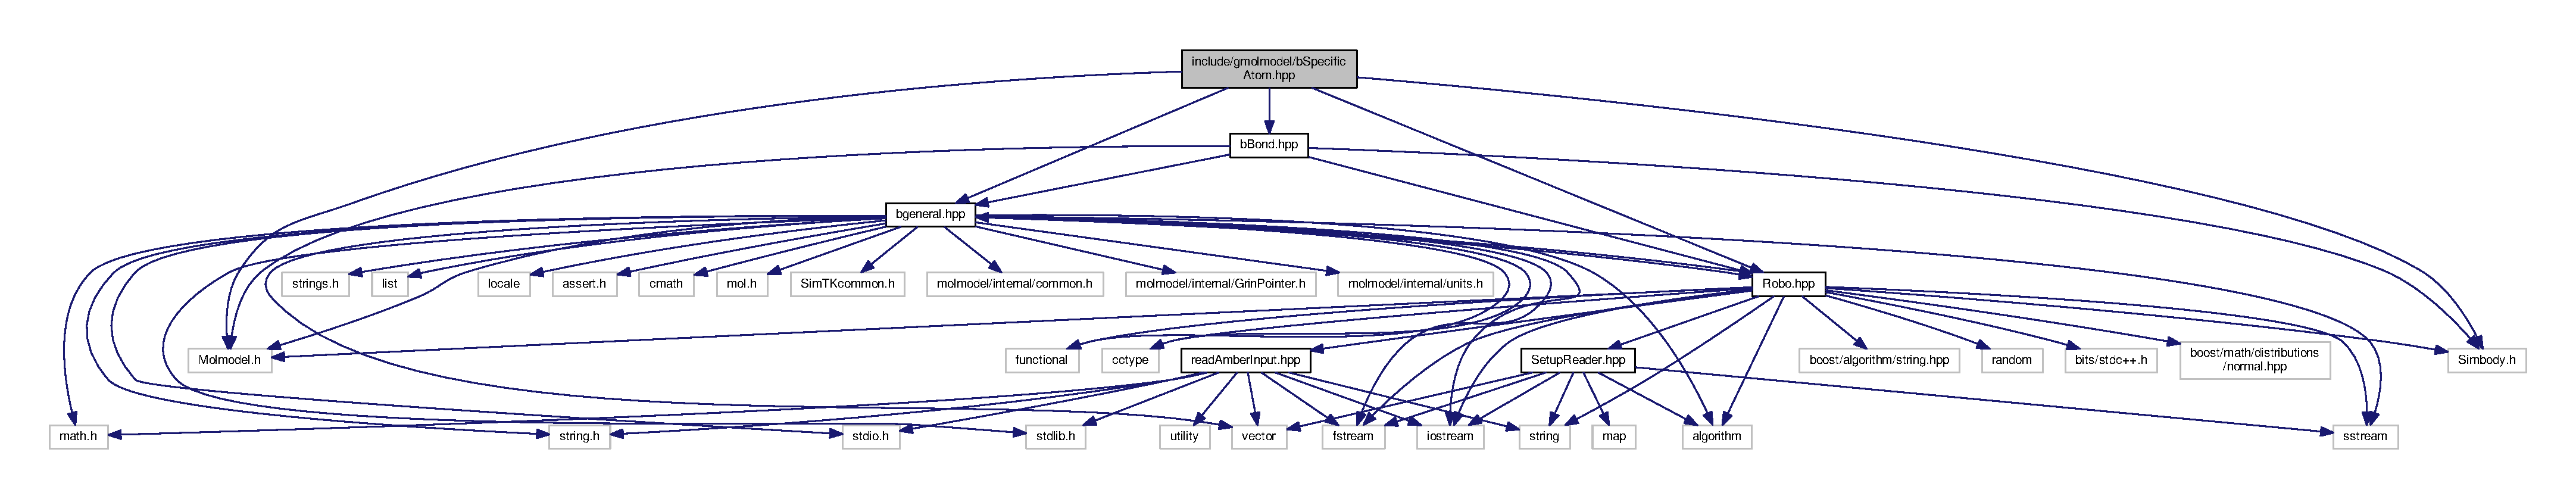
\includegraphics[width=350pt]{bSpecificAtom_8hpp__incl}
\end{center}
\end{figure}
This graph shows which files directly or indirectly include this file\+:
\nopagebreak
\begin{figure}[H]
\begin{center}
\leavevmode
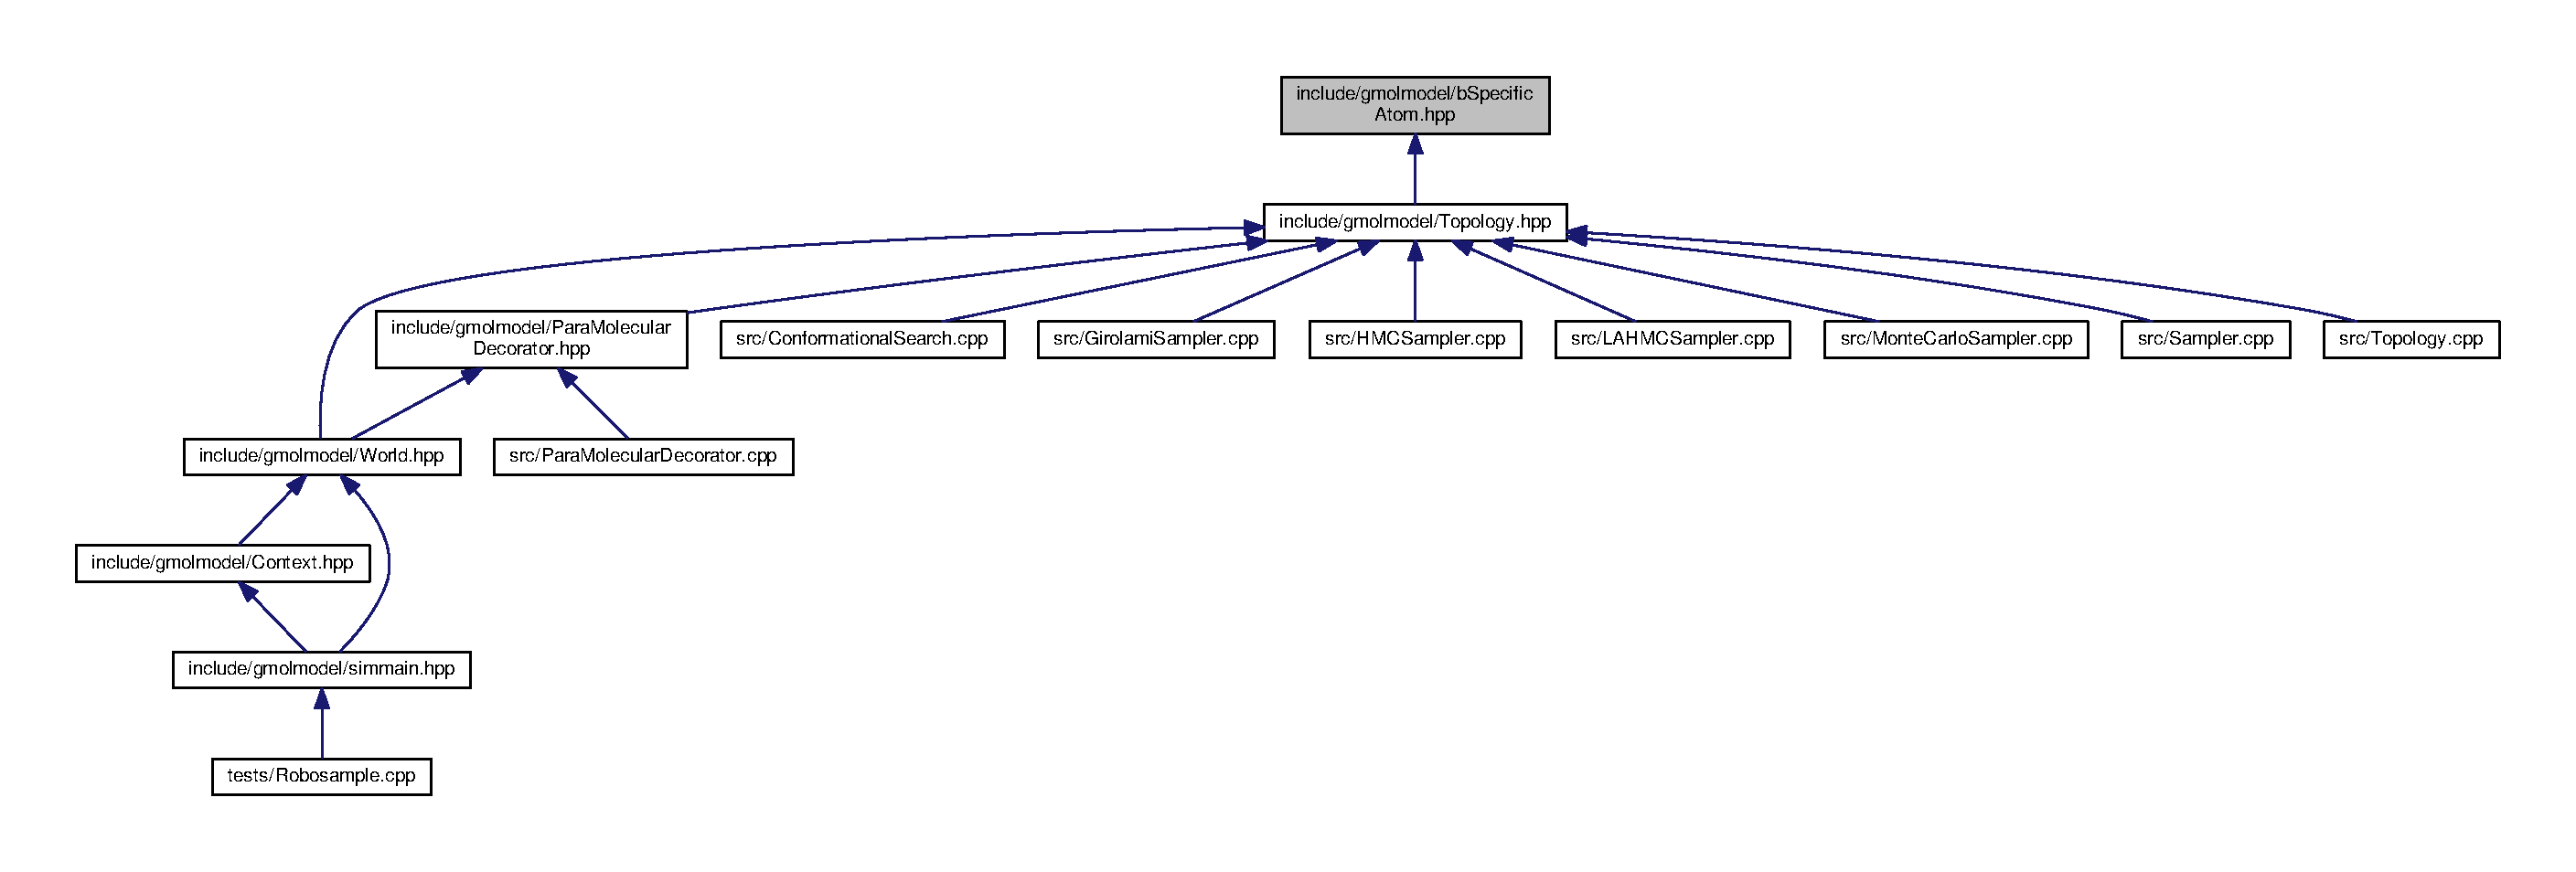
\includegraphics[width=350pt]{bSpecificAtom_8hpp__dep__incl}
\end{center}
\end{figure}
\subsection*{Classes}
\begin{DoxyCompactItemize}
\item 
class \hyperlink{classbSpecificAtom}{b\+Specific\+Atom}
\end{DoxyCompactItemize}
\subsection*{Functions}
\begin{DoxyCompactItemize}
\item 
int {\bfseries b\+Atom\+Assign} (Mol\+Atom $\ast$dest, const \hyperlink{classbSpecificAtom}{b\+Specific\+Atom} $\ast$src)\hypertarget{bSpecificAtom_8hpp_a76fb487ed90987fdafce2eca8b2b566c}{}\label{bSpecificAtom_8hpp_a76fb487ed90987fdafce2eca8b2b566c}

\end{DoxyCompactItemize}


\subsection{Detailed Description}
This defines the b\+Molecule\+Reader class and additional heloer classes 
\hypertarget{TrivalentAtomTetra_8hpp}{}\section{include/gmolmodel/\+Trivalent\+Atom\+Tetra.hpp File Reference}
\label{TrivalentAtomTetra_8hpp}\index{include/gmolmodel/\+Trivalent\+Atom\+Tetra.\+hpp@{include/gmolmodel/\+Trivalent\+Atom\+Tetra.\+hpp}}
{\ttfamily \#include \char`\"{}Robo.\+hpp\char`\"{}}\\*
{\ttfamily \#include \char`\"{}Simbody.\+h\char`\"{}}\\*
{\ttfamily \#include \char`\"{}Molmodel.\+h\char`\"{}}\\*
Include dependency graph for Trivalent\+Atom\+Tetra.\+hpp\+:\nopagebreak
\begin{figure}[H]
\begin{center}
\leavevmode
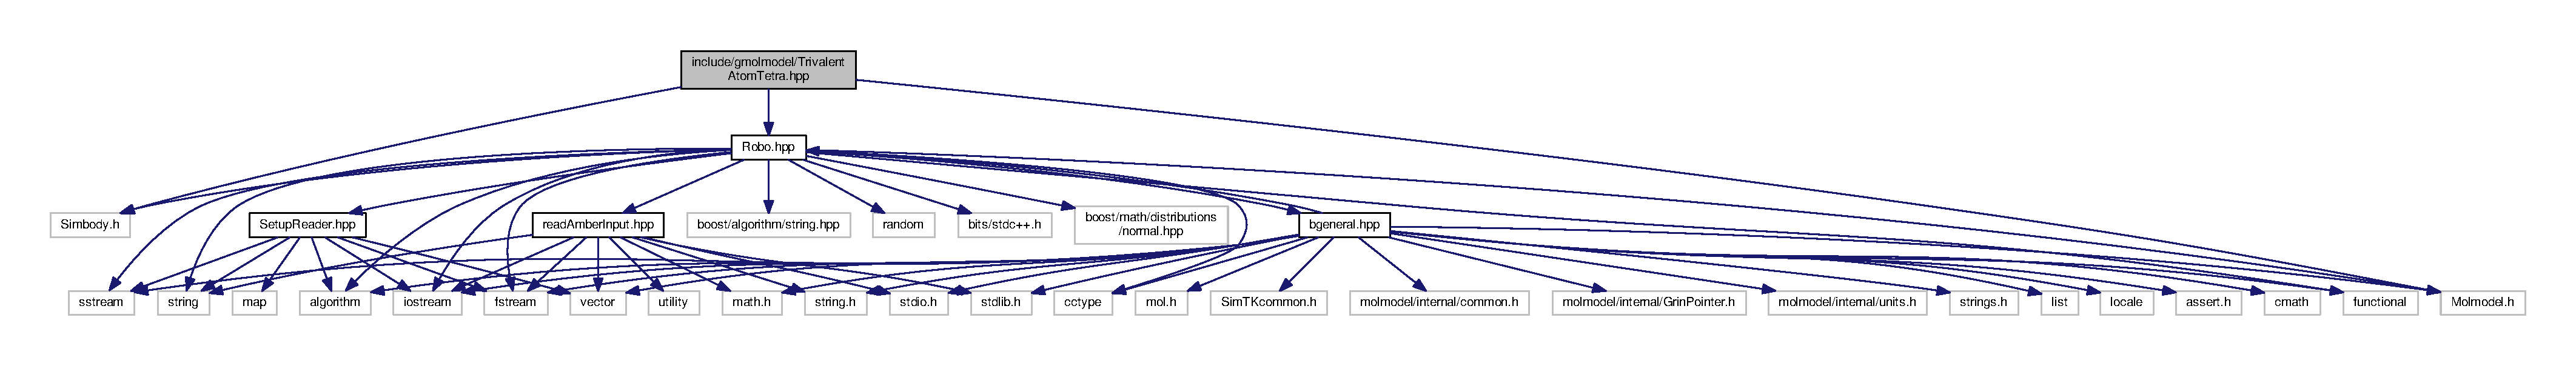
\includegraphics[width=350pt]{TrivalentAtomTetra_8hpp__incl}
\end{center}
\end{figure}
This graph shows which files directly or indirectly include this file\+:
\nopagebreak
\begin{figure}[H]
\begin{center}
\leavevmode
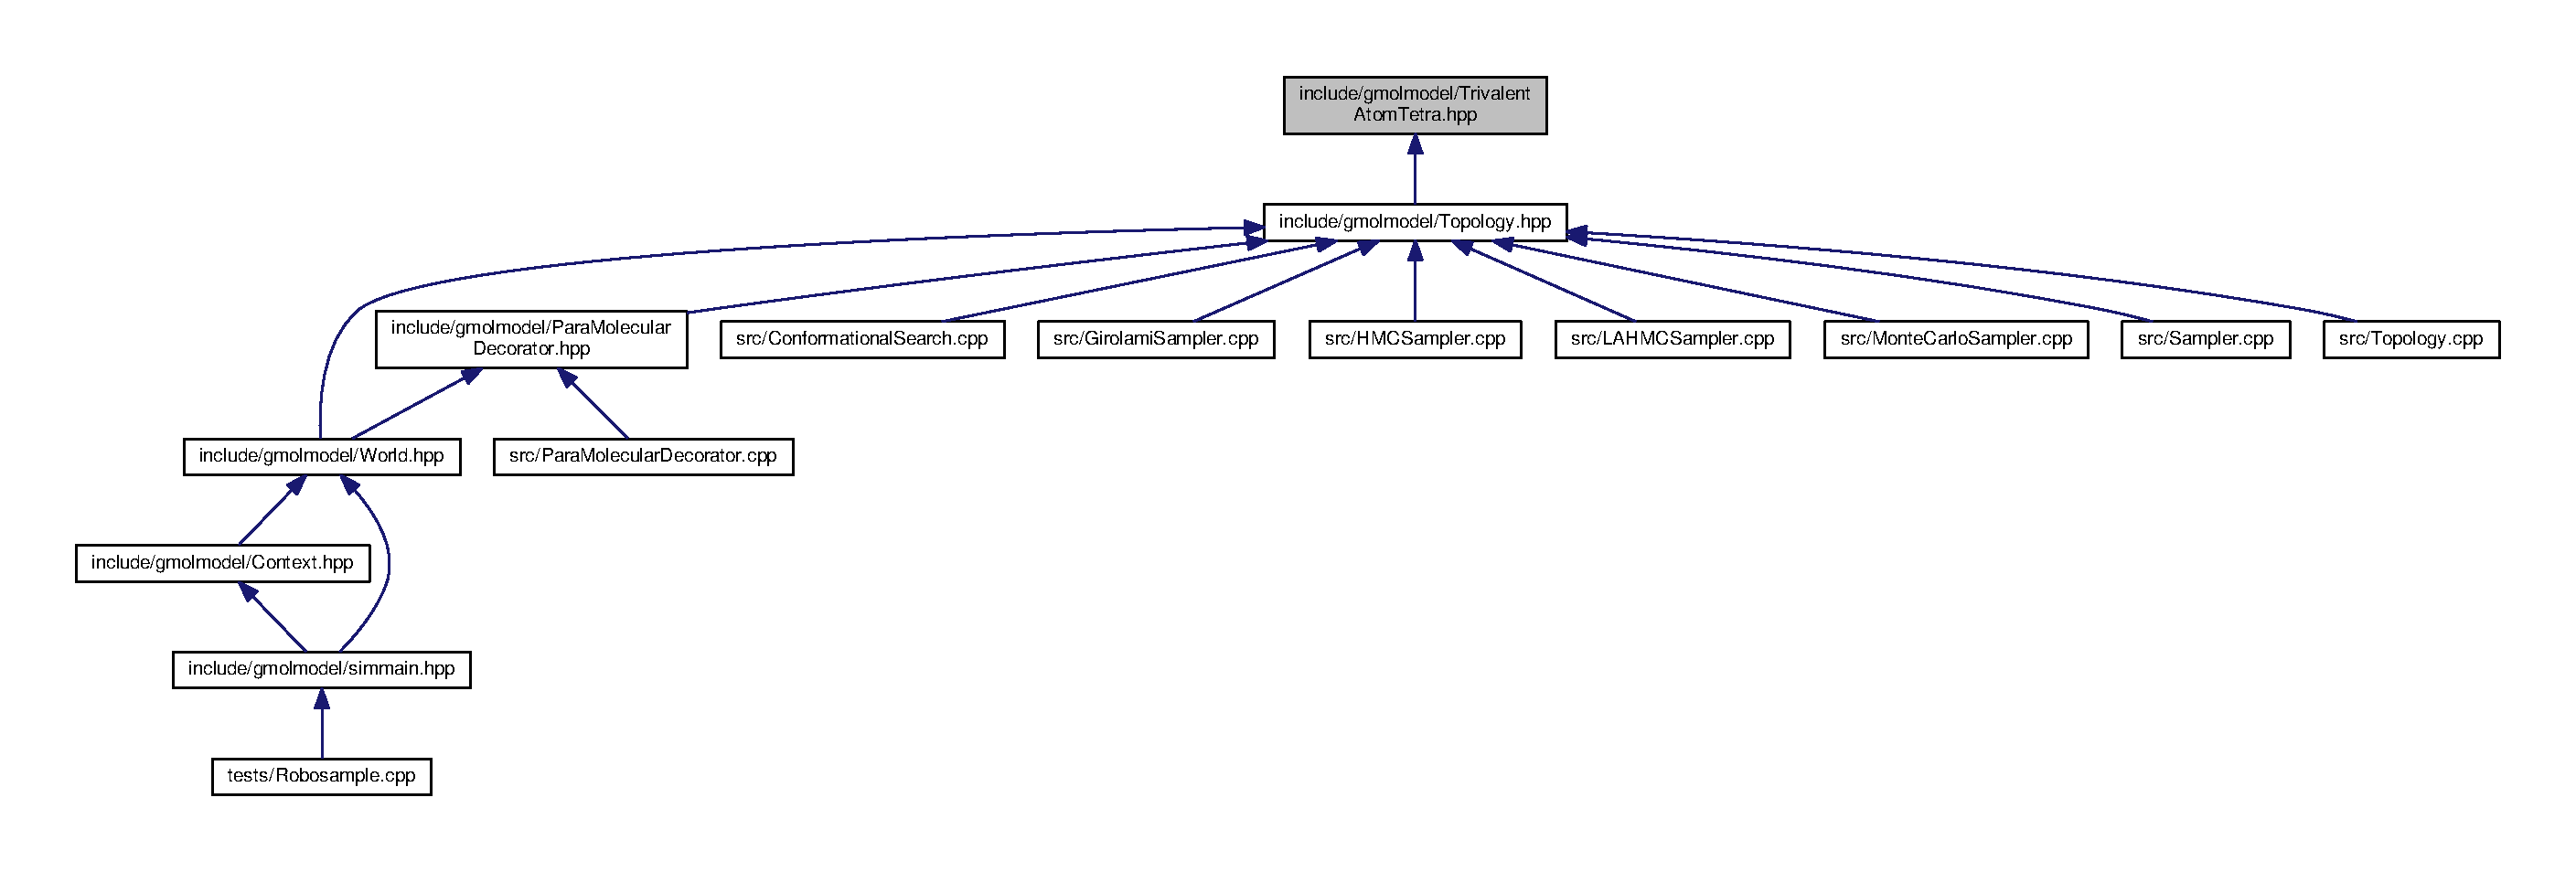
\includegraphics[width=350pt]{TrivalentAtomTetra_8hpp__dep__incl}
\end{center}
\end{figure}
\subsection*{Classes}
\begin{DoxyCompactItemize}
\item 
class \hyperlink{classTrivalentAtomTetra}{Trivalent\+Atom\+Tetra}
\end{DoxyCompactItemize}


\subsection{Detailed Description}
This defines the \hyperlink{classTrivalentAtomTetra}{Trivalent\+Atom\+Tetra} class 
\hypertarget{bArgParser_8cpp}{}\section{src/b\+Arg\+Parser.cpp File Reference}
\label{bArgParser_8cpp}\index{src/b\+Arg\+Parser.\+cpp@{src/b\+Arg\+Parser.\+cpp}}
{\ttfamily \#include \char`\"{}b\+Arg\+Parser.\+hpp\char`\"{}}\\*
Include dependency graph for b\+Arg\+Parser.\+cpp\+:\nopagebreak
\begin{figure}[H]
\begin{center}
\leavevmode
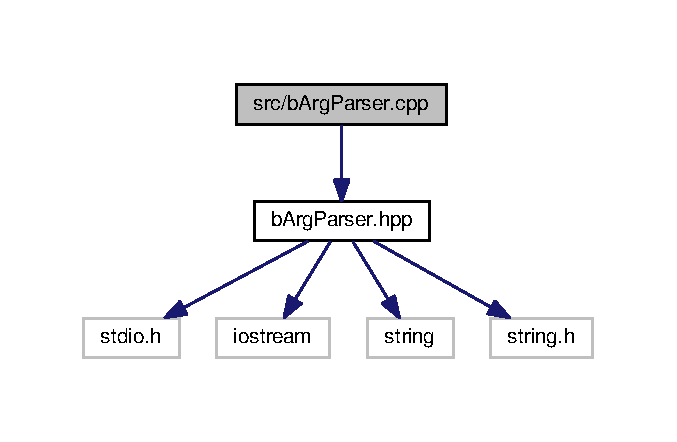
\includegraphics[width=325pt]{bArgParser_8cpp__incl}
\end{center}
\end{figure}


\subsection{Detailed Description}
Implementation of \hyperlink{classbArgParser}{b\+Arg\+Parser} class. 
\hypertarget{ConformationalSearch_8cpp}{}\section{src/\+Conformational\+Search.cpp File Reference}
\label{ConformationalSearch_8cpp}\index{src/\+Conformational\+Search.\+cpp@{src/\+Conformational\+Search.\+cpp}}
{\ttfamily \#include \char`\"{}Conformational\+Search.\+hpp\char`\"{}}\\*
{\ttfamily \#include \char`\"{}Topology.\+hpp\char`\"{}}\\*
Include dependency graph for Conformational\+Search.\+cpp\+:\nopagebreak
\begin{figure}[H]
\begin{center}
\leavevmode
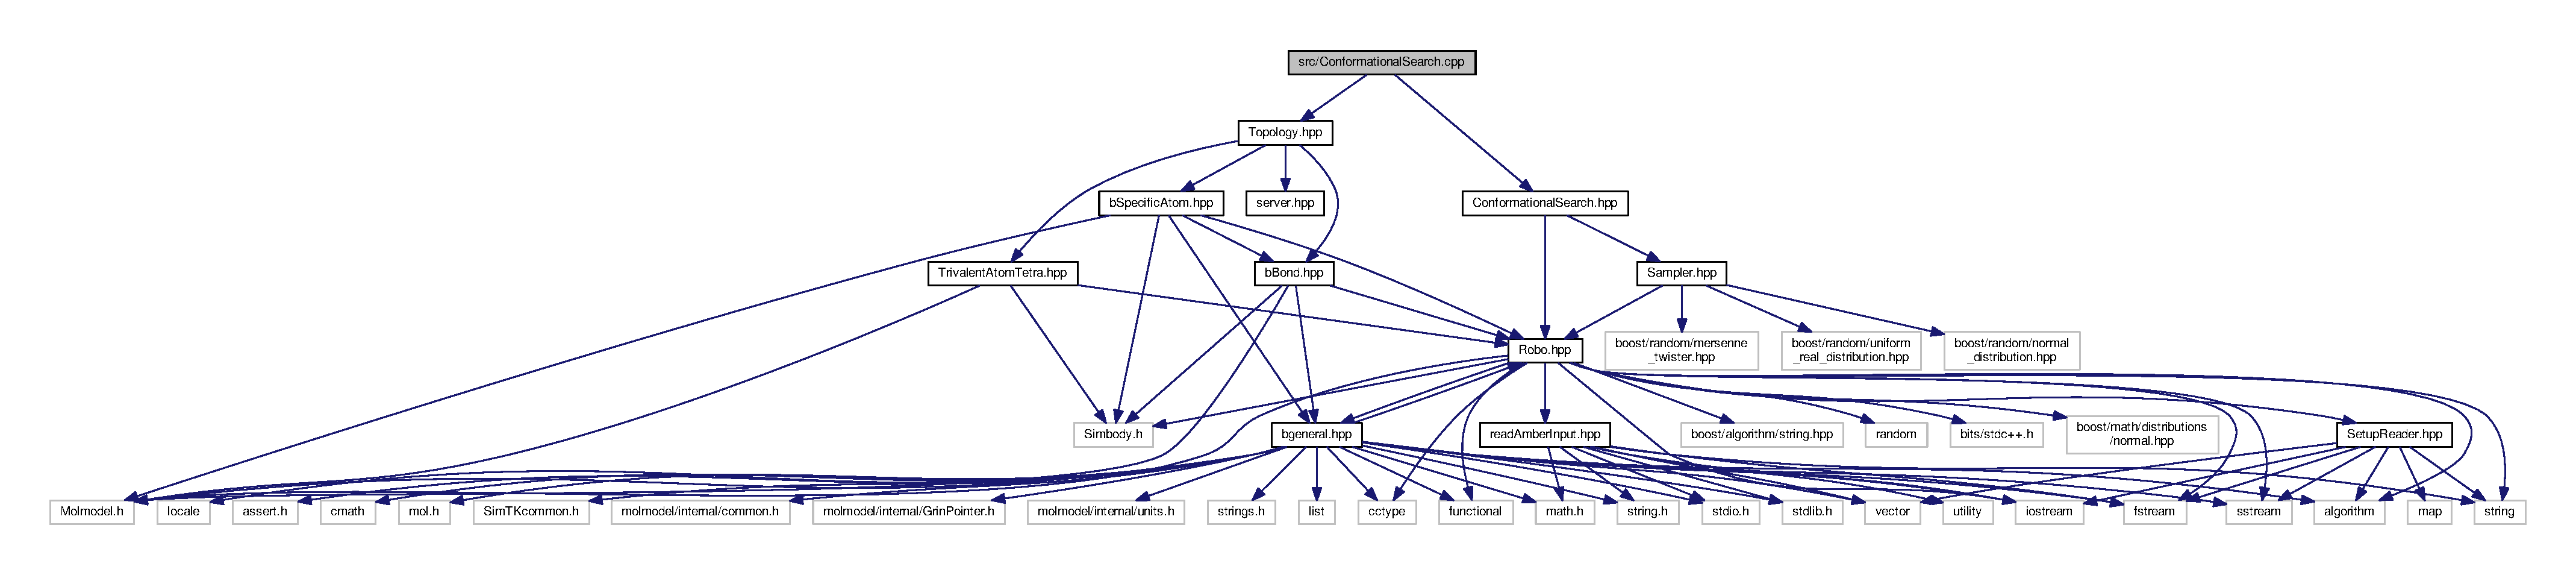
\includegraphics[width=350pt]{ConformationalSearch_8cpp__incl}
\end{center}
\end{figure}


\subsection{Detailed Description}
Implementation of \hyperlink{classConformationalSearch}{Conformational\+Search} class. 
\hypertarget{GirolamiSampler_8cpp}{}\section{src/\+Girolami\+Sampler.cpp File Reference}
\label{GirolamiSampler_8cpp}\index{src/\+Girolami\+Sampler.\+cpp@{src/\+Girolami\+Sampler.\+cpp}}
{\ttfamily \#include \char`\"{}Girolami\+Sampler.\+hpp\char`\"{}}\\*
{\ttfamily \#include \char`\"{}Topology.\+hpp\char`\"{}}\\*
Include dependency graph for Girolami\+Sampler.\+cpp\+:\nopagebreak
\begin{figure}[H]
\begin{center}
\leavevmode
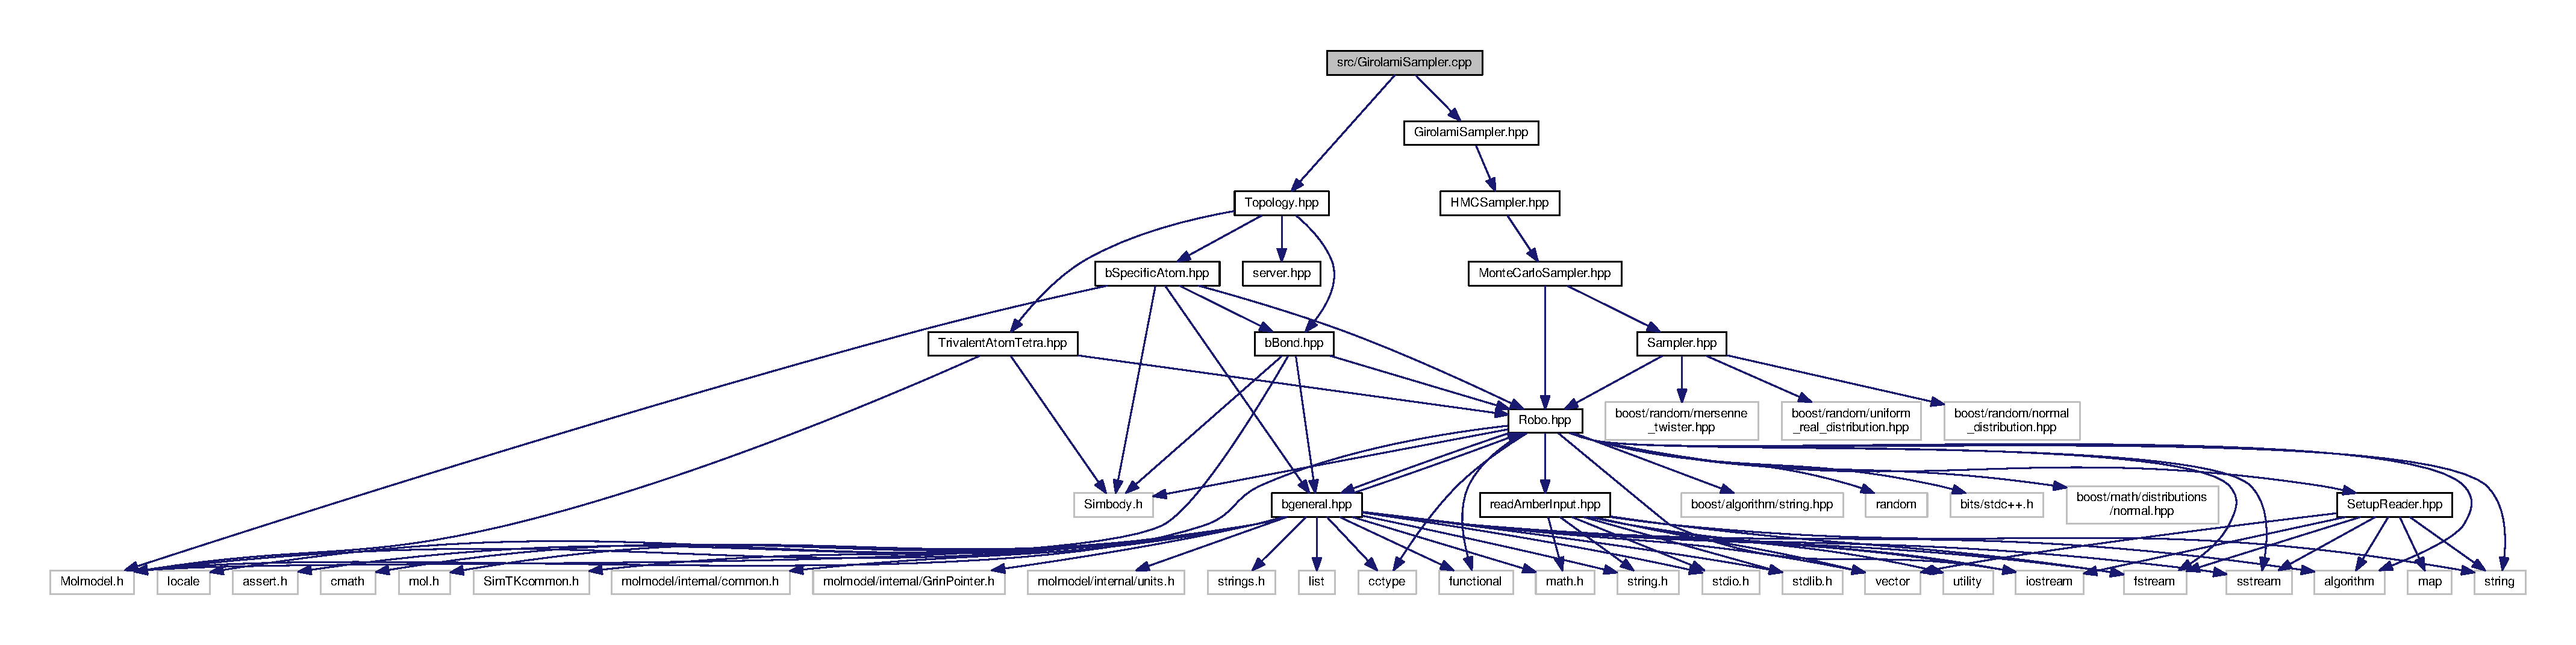
\includegraphics[width=350pt]{GirolamiSampler_8cpp__incl}
\end{center}
\end{figure}


\subsection{Detailed Description}
Implementation of \hyperlink{classGirolamiSampler}{Girolami\+Sampler} class. 
\hypertarget{HMCSampler_8cpp}{}\section{src/\+H\+M\+C\+Sampler.cpp File Reference}
\label{HMCSampler_8cpp}\index{src/\+H\+M\+C\+Sampler.\+cpp@{src/\+H\+M\+C\+Sampler.\+cpp}}
{\ttfamily \#include \char`\"{}H\+M\+C\+Sampler.\+hpp\char`\"{}}\\*
{\ttfamily \#include \char`\"{}Topology.\+hpp\char`\"{}}\\*
Include dependency graph for H\+M\+C\+Sampler.\+cpp\+:\nopagebreak
\begin{figure}[H]
\begin{center}
\leavevmode
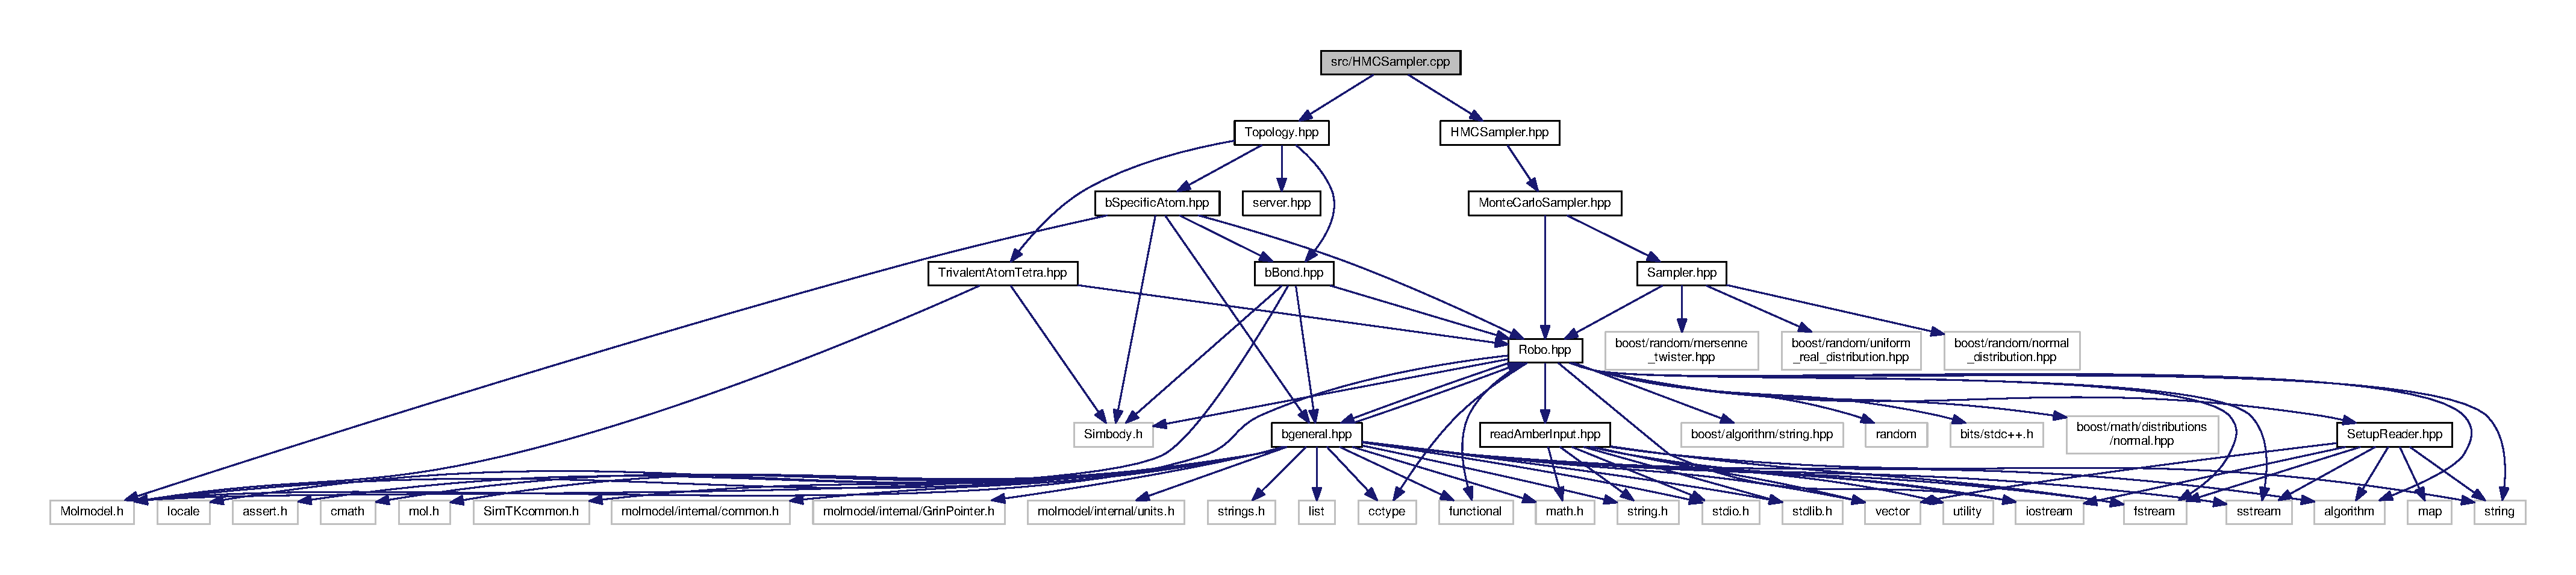
\includegraphics[width=350pt]{HMCSampler_8cpp__incl}
\end{center}
\end{figure}


\subsection{Detailed Description}
Implementation of \hyperlink{classHMCSampler}{H\+M\+C\+Sampler} class. 
\hypertarget{LAHMCSampler_8cpp}{}\section{src/\+L\+A\+H\+M\+C\+Sampler.cpp File Reference}
\label{LAHMCSampler_8cpp}\index{src/\+L\+A\+H\+M\+C\+Sampler.\+cpp@{src/\+L\+A\+H\+M\+C\+Sampler.\+cpp}}
{\ttfamily \#include \char`\"{}L\+A\+H\+M\+C\+Sampler.\+hpp\char`\"{}}\\*
{\ttfamily \#include \char`\"{}Topology.\+hpp\char`\"{}}\\*
Include dependency graph for L\+A\+H\+M\+C\+Sampler.\+cpp\+:\nopagebreak
\begin{figure}[H]
\begin{center}
\leavevmode
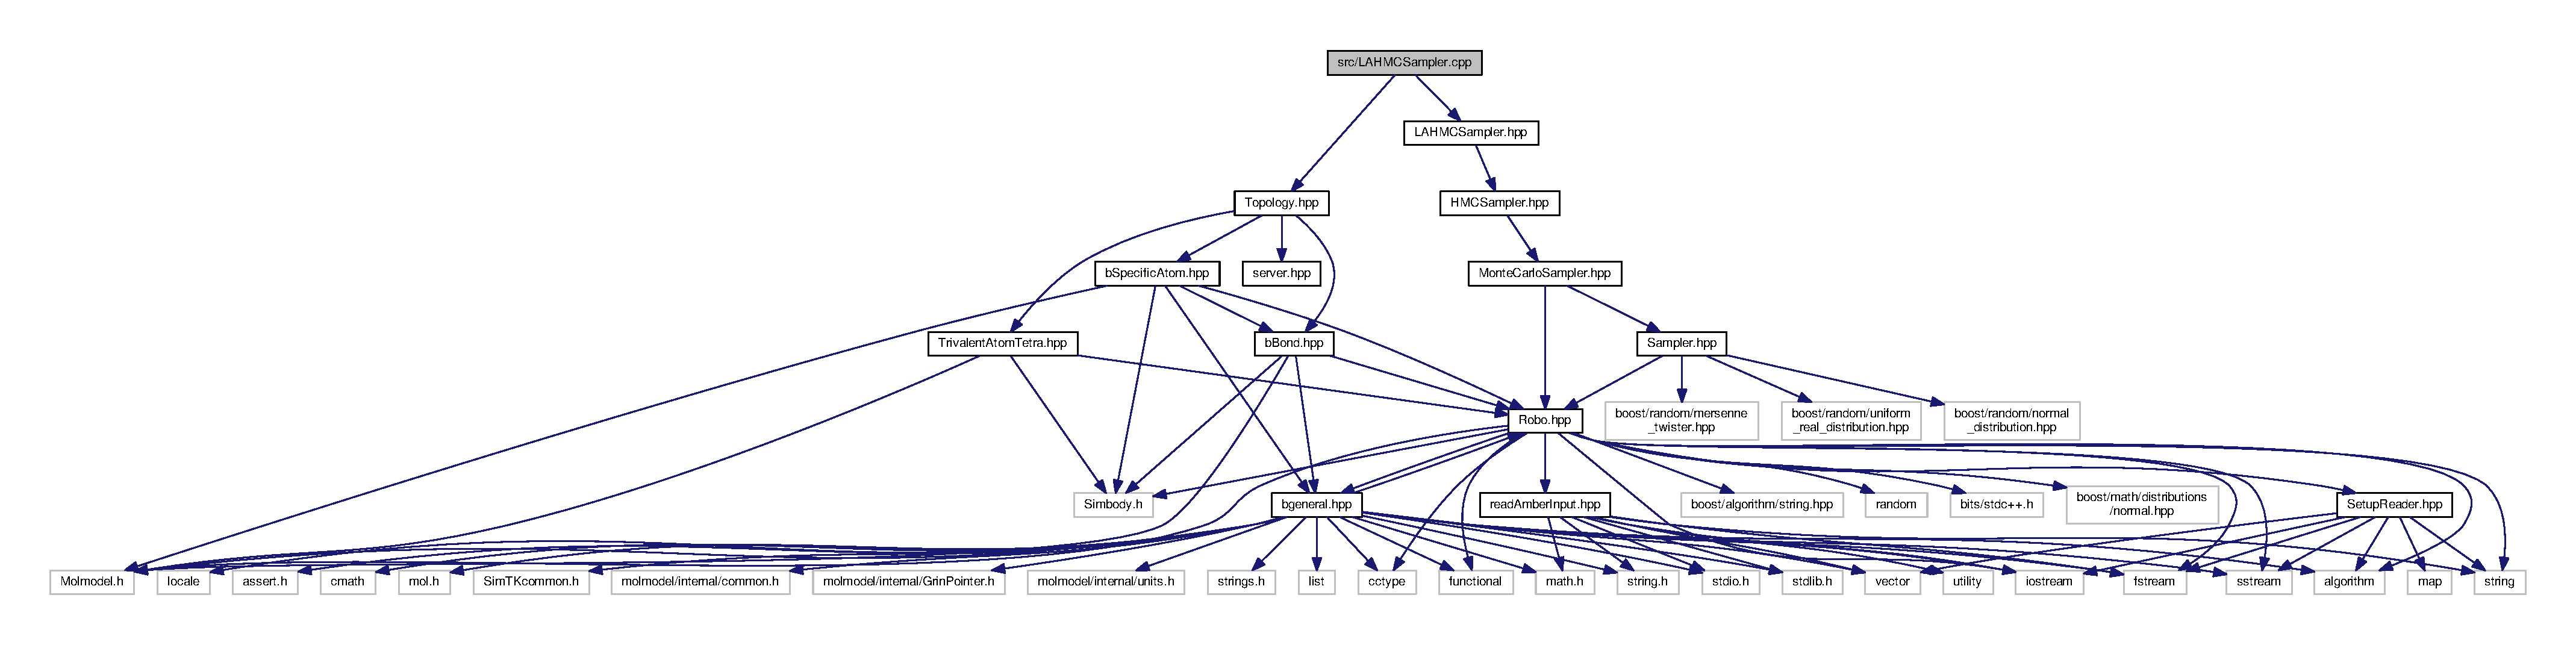
\includegraphics[width=350pt]{LAHMCSampler_8cpp__incl}
\end{center}
\end{figure}


\subsection{Detailed Description}
Implementation of \hyperlink{classLAHMCSampler}{L\+A\+H\+M\+C\+Sampler} class. 
\hypertarget{MonteCarloSampler_8cpp}{}\section{src/\+Monte\+Carlo\+Sampler.cpp File Reference}
\label{MonteCarloSampler_8cpp}\index{src/\+Monte\+Carlo\+Sampler.\+cpp@{src/\+Monte\+Carlo\+Sampler.\+cpp}}
{\ttfamily \#include \char`\"{}Monte\+Carlo\+Sampler.\+hpp\char`\"{}}\\*
{\ttfamily \#include \char`\"{}Topology.\+hpp\char`\"{}}\\*
Include dependency graph for Monte\+Carlo\+Sampler.\+cpp\+:\nopagebreak
\begin{figure}[H]
\begin{center}
\leavevmode
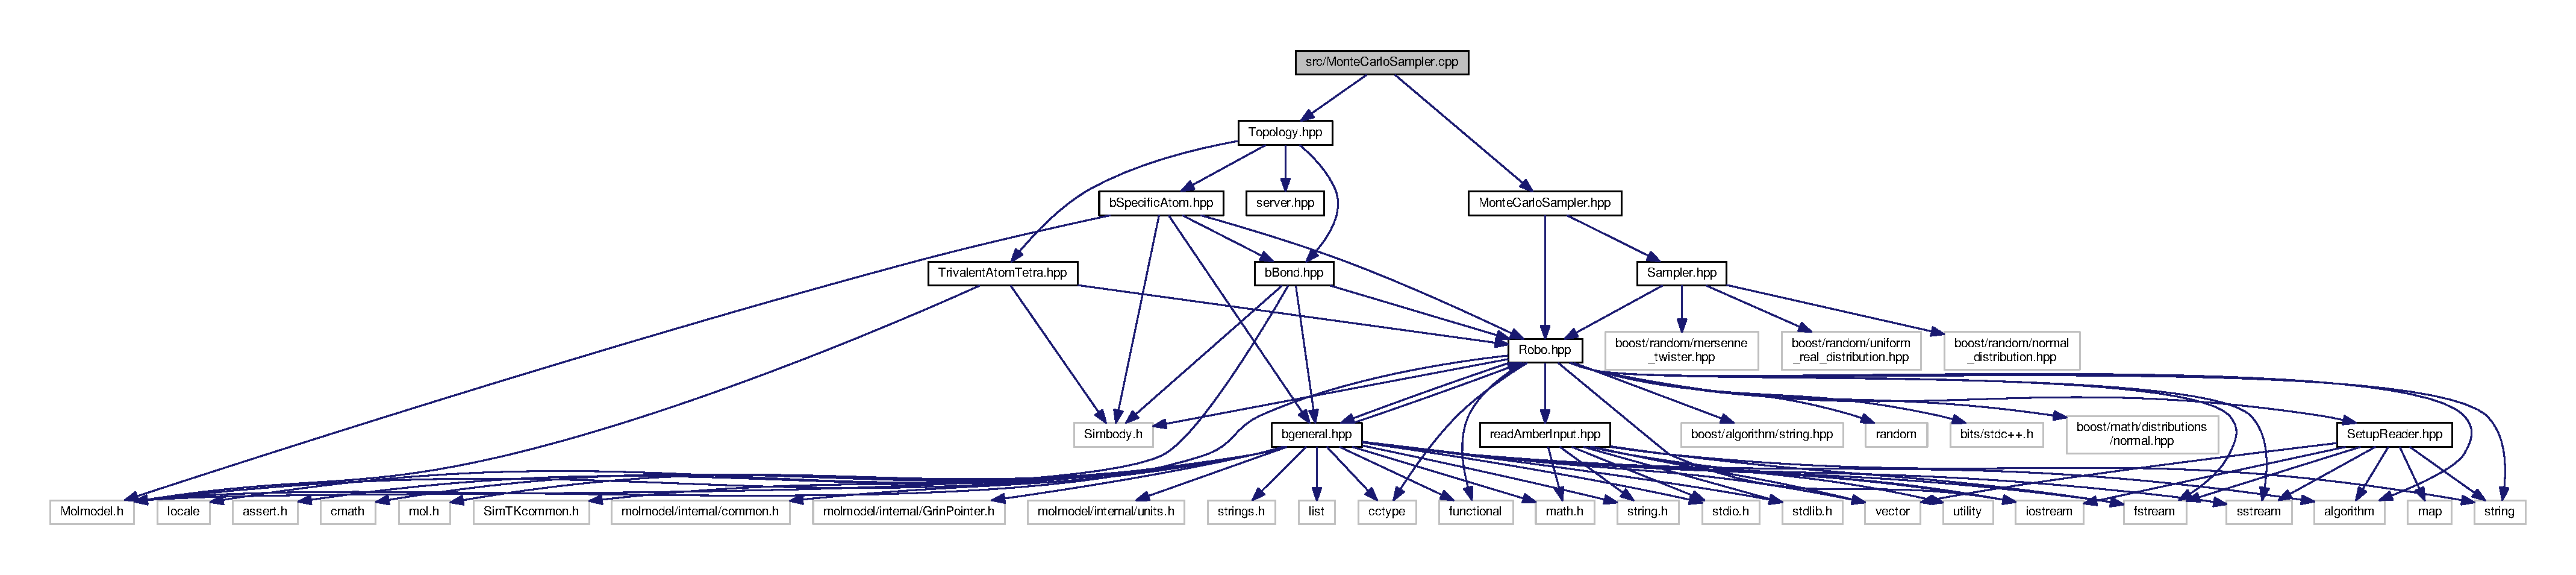
\includegraphics[width=350pt]{MonteCarloSampler_8cpp__incl}
\end{center}
\end{figure}


\subsection{Detailed Description}
Implementation of \hyperlink{classMonteCarloSampler}{Monte\+Carlo\+Sampler} class. 
\hypertarget{ParaMolecularDecorator_8cpp}{}\section{src/\+Para\+Molecular\+Decorator.cpp File Reference}
\label{ParaMolecularDecorator_8cpp}\index{src/\+Para\+Molecular\+Decorator.\+cpp@{src/\+Para\+Molecular\+Decorator.\+cpp}}
{\ttfamily \#include \char`\"{}Robo.\+hpp\char`\"{}}\\*
{\ttfamily \#include \char`\"{}Para\+Molecular\+Decorator.\+hpp\char`\"{}}\\*
Include dependency graph for Para\+Molecular\+Decorator.\+cpp\+:\nopagebreak
\begin{figure}[H]
\begin{center}
\leavevmode
\includegraphics[width=350pt]{ParaMolecularDecorator_8cpp__incl}
\end{center}
\end{figure}


\subsection{Detailed Description}
Implementation of \hyperlink{classHMCSampler}{H\+M\+C\+Sampler} class. 
\hypertarget{Sampler_8cpp}{}\section{src/\+Sampler.cpp File Reference}
\label{Sampler_8cpp}\index{src/\+Sampler.\+cpp@{src/\+Sampler.\+cpp}}
{\ttfamily \#include \char`\"{}Sampler.\+hpp\char`\"{}}\\*
{\ttfamily \#include \char`\"{}Topology.\+hpp\char`\"{}}\\*
Include dependency graph for Sampler.\+cpp\+:\nopagebreak
\begin{figure}[H]
\begin{center}
\leavevmode
\includegraphics[width=350pt]{Sampler_8cpp__incl}
\end{center}
\end{figure}


\subsection{Detailed Description}
Implementation of \hyperlink{classSampler}{Sampler} class. 
\hypertarget{Topology_8cpp}{}\section{src/\+Topology.cpp File Reference}
\label{Topology_8cpp}\index{src/\+Topology.\+cpp@{src/\+Topology.\+cpp}}
{\ttfamily \#include \char`\"{}Topology.\+hpp\char`\"{}}\\*
Include dependency graph for Topology.\+cpp\+:\nopagebreak
\begin{figure}[H]
\begin{center}
\leavevmode
\includegraphics[width=350pt]{Topology_8cpp__incl}
\end{center}
\end{figure}


\subsection{Detailed Description}
Implementation of \hyperlink{classTopology}{Topology} class. 
\hypertarget{Robosample_8cpp}{}\section{tests/\+Robosample.cpp File Reference}
\label{Robosample_8cpp}\index{tests/\+Robosample.\+cpp@{tests/\+Robosample.\+cpp}}
{\ttfamily \#include $<$string$>$}\\*
{\ttfamily \#include $<$iostream$>$}\\*
{\ttfamily \#include $<$sstream$>$}\\*
{\ttfamily \#include $<$chrono$>$}\\*
{\ttfamily \#include $<$cassert$>$}\\*
{\ttfamily \#include $<$sys/stat.\+h$>$}\\*
{\ttfamily \#include \char`\"{}simmain.\+hpp\char`\"{}}\\*
{\ttfamily \#include \char`\"{}Robo.\+hpp\char`\"{}}\\*
{\ttfamily \#include \char`\"{}H\+M\+C\+Sampler.\+hpp\char`\"{}}\\*
{\ttfamily \#include \char`\"{}read\+Amber\+Input.\+hpp\char`\"{}}\\*
{\ttfamily \#include \char`\"{}Setup\+Reader.\+hpp\char`\"{}}\\*
Include dependency graph for Robosample.\+cpp\+:
\nopagebreak
\begin{figure}[H]
\begin{center}
\leavevmode
\includegraphics[width=350pt]{Robosample_8cpp__incl}
\end{center}
\end{figure}
\subsection*{Functions}
\begin{DoxyCompactItemize}
\item 
void {\bfseries Print\+Help} ()\hypertarget{Robosample_8cpp_ae964ff8411b4fdcaf65cb5529aea4bef}{}\label{Robosample_8cpp_ae964ff8411b4fdcaf65cb5529aea4bef}

\item 
int {\bfseries main} (int argc, char $\ast$$\ast$argv)\hypertarget{Robosample_8cpp_a3c04138a5bfe5d72780bb7e82a18e627}{}\label{Robosample_8cpp_a3c04138a5bfe5d72780bb7e82a18e627}

\end{DoxyCompactItemize}


\subsection{Detailed Description}
This file tests the \hyperlink{classContext}{Context} class 
%--- End generated contents ---

% Index
\backmatter
\newpage
\phantomsection
\clearemptydoublepage
\addcontentsline{toc}{chapter}{Index}
\printindex

\end{document}
